%% LaTeX2e class for student theses
%% thesis.tex
%% 
%% Karlsruhe Institute of Technology
%% Institute for Program Structures and Data Organization
%% Chair for Software Design and Quality (SDQ)
%%
%% Dr.-Ing. Erik Burger
%% burger@kit.edu
%%
%% See https://sdq.kastel.kit.edu/wiki/Dokumentvorlagen
%%
%% Version 1.3.6, 2022-09-28

%% Available page modes: oneside, twoside
%% Available languages: english, ngerman
%% Available modes: draft, final (see README)
\documentclass[oneside, english]{sdqthesis}

%% ---------------------------------
%% | Information about the thesis  |
%% ---------------------------------

%% Name of the author
\author{Felix Möller}

%% Title (and possibly subtitle) of the thesis
\title{Continual Active Learning for Effective Model Stealing Attacks}

%% Type of the thesis 
\thesistype{Bachelor's Thesis}

%% Change the institute here, ``KASTEL'' is default
% \myinstitute{Institute for \dots}

%% You can put a logo in the ``logos'' directory and include it here
%% instead of the SDQ logo
% \grouplogo{myfile}
%% Alternatively, you can disable the group logo
% \nogrouplogo

%% The reviewers are the professors that grade your thesis
\reviewerone{Jun.-Prof. Dr. Christian Wressnegger}
\reviewertwo{Prof. Dr. Thorsten Strufe}

%% The advisors are PhDs or Postdocs
\advisorone{M.Sc. Yilin Ji}
%% The second advisor can be omitted
\advisortwo{}

%% Please enter the start end end time of your thesis
\editingtime{10. January 2023}{10. May 2023}

\settitle

%% --------------------------------
%% | Bibliography                 |
%% --------------------------------

%% Use biber instead of BibTeX, see README
%\usepackage[nonumberlist,toc]{glossaries} 
\usepackage[nonumberlist,nopostdot]{glossaries} 
\makeglossaries



\newglossaryentry{Hallo}{
    name={Hallo},
    plural={Hallos},
    description={Dies ist ein Test.}
}

\newglossaryentry{Cold Start}{
    % Explain difference to warm start
    name={Cold Start},
    plural={Cold Starts},
    description={Cold Start is a term used in Active Learning literature and }
}

\newglossaryentry{Batch Size}{
    name={Abc},
    plural={Def},
    description={GHI}
}

\newglossaryentry{ActiveThiefConv}{
    name={ActiveThiefConv},
    plural={ActiveThiefConvs},
    description={proprietary Convolutional Neural Network Architecture used in the ActiveThief framework. ActiveThiefConv consists of 2,3 or 4 convolution blocks followed  by a fully connected layer. The architecture is shown in TODO }
    %\cite{pal2020activethief}.
}

\newglossaryentry{SmallImagenet}{
    name={SmallImagenet},
    plural={SmallImagenets},
    description={A subset of the ImageNet TODO.}
}
\usepackage{dsfont}
\usepackage{hyperref}
\usepackage{tabularx}
\usepackage[citestyle=numeric,style=numeric,backend=biber]{biblatex}
\usepackage{algorithm}
\usepackage{algpseudocode}
%\renewcommand{\algorithmicrequire}{\textbf{Input:}}
\renewcommand{\algorithmicrequire}{\textbf{Input:}}
\newcommand{\algorithmicoutput}{\textbf{return}}
\newcommand{\return}{\item[\algorithmicoutput]}
\usepackage{amsmath}
\usepackage{amsthm}
\usepackage{makecell}
\newtheorem{theorem}{Theorem}
\usepackage{commath}
\usepackage{diagbox}
\usepackage{multirow}
\DeclareMathOperator*{\argmax}{\arg\!\max}
\DeclareMathOperator*{\argmin}{\arg\!\min}
\addbibresource{thesis.bib}

%% ====================================
%% ====================================
%% ||                                ||
%% || Beginning of the main document ||
%% ||                                ||
%% ====================================
%% ====================================
\begin{document}

%% Set PDF metadata
\setpdf

%% Set the title
\maketitle

%% The Preamble begins here
\frontmatter

%% LaTeX2e class for student theses: Declaration of independent work
%% sections/declaration.tex
%% 
%% Karlsruhe Institute of Technology
%% Institute for Program Structures and Data Organization
%% Chair for Software Design and Quality (SDQ)
%%
%% Dr.-Ing. Erik Burger
%% burger@kit.edu
%%
%% Version 1.3.6, 2022-09-28

\thispagestyle{empty}
\null\vfill
\noindent\hbox to \textwidth{\hrulefill} 
\iflanguage{english}{I declare that I have developed and written the enclosed
thesis completely by myself. I have submitted neither parts of nor the complete 
thesis as an examination elsewhere. I have not used any other than the aids that
I have mentioned. I have marked all parts of the thesis that I have included from 
referenced literature, either in their original wording or paraphrasing their
contents. This also applies to figures, sketches, images and similar depictions,
as well as sources from the internet.}%
{Ich versichere hiermit, dass ich die vorliegende Arbeit selbstständig verfasst,
und weder ganz oder in Teilen als Prüfungsleistung vorgelegt und keine anderen
als die angegebenen Hilfsmittel benutzt habe. Sämtliche Stellen der Arbeit, die
benutzten Werken im Wortlaut oder dem Sinn nach entnommen sind, habe ich durch
Quellenangaben kenntlich gemacht. Dies gilt auch für Zeichnungen, Skizzen,
bildliche Darstellungen und dergleichen sowie für Quellen aus dem Internet. }
 
 
%% ---------------------------------------------
%% | Replace PLACE and DATE with actual values |
%% ---------------------------------------------
\textbf{Karlsruhe, May 10th,2023}
\vspace{1.5cm}
 
\dotfill\hspace*{8.0cm}\\
\hspace*{2cm}(\theauthor) 
\cleardoublepage

\setcounter{page}{1}
\pagenumbering{roman}

%% ----------------
%% |   Abstract   |
%% ----------------
 
%% For theses written in English, an abstract both in English
%% and German is mandatory.
%%
%% For theses written in German, a German abstract is sufficient.
%%
%% The text is included from the following files:
%% - sections/abstract

\includeabstract
\printglossaries
\chapter*{Notation}
\label{ch:notation}

% Mention b as batch size

This chapter is intended as a quick overview of the mathematical notation used in this work.
The symbols largely follow contemporary works, while simultaneously trying to avoid ambiguity.
Furthermore, the notation refrains from assigning semantics to different font weights, in order to stay consistent across multiple media.

\begin{tabularx}{\textwidth}{l X}
    \toprule
    Symbol & Definition \\
    \midrule
    $y_i$ & The label of the given data point $x_i$, also known as $y(x_i)$. \\ \addlinespace
    $T$ & Number of ... \\ \addlinespace
    \bottomrule
\end{tabularx}
\label{tab:notation}

%% ------------------------
%% |   Table of Contents  |
%% ------------------------
\tableofcontents

\listoffigures
\listoftables

%% -----------------
%% |   Main part   |
%% -----------------

\mainmatter

\glsresetall
%% LaTeX2e class for student theses
%% sections/content.tex
%% 
%% Karlsruhe Institute of Technology
%% Institute for Program Structures and Data Organization
%% Chair for Software Design and Quality (SDQ)
%%
%% Dr.-Ing. Erik Burger
%% burger@kit.edu
%%
%% Version 1.3.6, 2022-09-28

\chapter{Introduction}
\label{ch:Introduction}

%% -------------------
%% | Example content |
%% -------------------

This is the SDQ thesis template.
For more information on the formatting of theses at SDQ, please refer to
\url{https://sdq.kastel.kit.edu/wiki/Ausarbeitungshinweise} or to your advisor.

\section{Spacing and indentation}
To separate parts of text in \LaTeX, please use two line breaks.
They will then be set with correct indentation.
Do \emph{not} use:
\begin{itemize}
  \itemsep0em
  \item \texttt{\textbackslash\textbackslash}
  \item \texttt{\textbackslash parskip}
  \item \texttt{\textbackslash vskip}
\end{itemize} 
or other commands to manually insert spaces, since they break the layout of this template.

\section{Example: Citation}
\label{sec:Introduction:Citation}
This template is based on \texttt{biblatex} and \texttt{biber}, which is preferred over the
outdated Bib\TeX{} software.
Please adjust your build environment if necessary (see
\url{https://sdq.kastel.kit.edu/wiki/BibTeX-Literaturlisten#biblatex.2Fbiber})

A citation: \cite{becker2008a} 

\section{Example: Figures}
\label{sec:Introduction:Figures}
\begin{figure}
\centering

\includegraphics[width=4cm]{logos/sdqlogo}
\caption{SDQ logo}
\label{fig:sdqlogo}
\end{figure}

A reference: The SDQ logo is displayed in \autoref{fig:sdqlogo}. 
(Use \code{\textbackslash autoref\{\}} for easy referencing.) 

\section{Example: Tables}
The \texttt{booktabs} package offers nicely typeset tables, as in \autoref{tab:atable}.

\label{sec:Introduction:Tables}
\begin{table}
\centering
\begin{tabular}{r l}
\toprule
abc & def\\
ghi & jkl\\
\midrule
123 & 456\\
789 & 0AB\\
\bottomrule
\end{tabular}
\caption{A table}
\label{tab:atable}
\end{table}

\section{Example: Formula}
One of the nice things about the Linux Libertine font is that it comes with
a math mode package.
\begin{displaymath}
f(x)=\Omega(g(x))\ (x\rightarrow\infty)\;\Leftrightarrow\;
\limsup_{x \to \infty} \left|\frac{f(x)}{g(x)}\right|> 0
\end{displaymath}

%% --------------------
%% | /Example content |
%% --------------------


\textbf{Contributions} \hspace{0.2cm} The objective of this thesis is to combine existing approaches of the continual learning domain
 with approaches in the active learning domain. More specifically, we are focusing on regularization-based continual learning methods
whereas we use both uncertainty-based and diversity-based active learning methods. The continual learning methods we use are Elastic
Weight Consolidation (EWC) \cite{Kirkpatrick2017}, Memory Aware Synapses (MAS) \cite{aljundi2018memory}, Incremental Moment Matching
(IMM) \cite{lee2017overcoming} and Asymmetric Loss Approximation by Single-Side Overestimation (ALASSO) \cite{park2019continual}.
Concerning active learning, we compare random sampling, Least Confidence (LC) \cite{lewis1994sequential} sampling, Batch Active Learning by
Diverse, uncertain Gradient lower Bound (BADGE) \cite{ash2019deep}, Bayesian Active Learning by Disagreement (BALD) \cite{houlsby2011bayesian} and
CoreSet \cite{sener2017active}.
We analyze how the continual learning methods can speed up the active learning process, which combinations of continual and active learning methods
are most effective and how the trade-off between accuracy and speed up is. While the focus of this thesis is on regularization-based continual
learning methods, we briefly explore the effectiveness of exemplar rehearsal continual learning using the Average Gradient Episodic Memory (AGEM)
approach \cite{chaudhry2018efficient} combined with representation-based active learning in form of Variational Adversarial Active Learning (VAAL)
\cite{sinha2019variational}. \\
After exploring the effectiveness of the different combinations of continual and active learning methods, we apply these combinations in the model stealing
domain. More specifically, we build upon the model extraction framework ActiveThief \cite{pal2020activethief} and investigate the performance of continual
active learning methods in the model stealing domain.

%% LaTeX2e class for student theses
%% sections/content.tex
%% 
%% Karlsruhe Institute of Technology
%% Institute for Program Structures and Data Organization
%% Chair for Software Design and Quality (SDQ)
%%
%% Dr.-Ing. Erik Burger
%% burger@kit.edu
%%
%% Version 1.3.6, 2022-09-28

\chapter{Background}
\label{ch:Background}

In this chapter we will give an overview of the background knowledge that is needed to understand the following chapters. The topic
of this thesis is at the intersection of the fields of Active Learning, Continual Learning and Model Stealing, and therefore we will
give an introduction to each of these fields. 

\section{Active Learning}
\label{sec:ActiveLearning}

%TODO: Hier learner-Beschreibung anpassen und ggf. Batch Active Learning einführen (Warum nötig? Für NNs)
% Representation-based active learning und diversity-based active learning sind quasi gleich, das noch erwähnen
Active Learning is a subfield of Machine Learning that focuses on the problem of how to select the most informative data points to label.
Research in Active Learning is motivated by the fact that data acquisition is often easy because it can be automated whereas labeling is
difficult and time-consuming. Therefore, the goal of research in Active Learning is to develop methods which maximize model performance
with minimal amount of labeled data. A typical Active Learning scenario comprises a learner, an oracle, unlabeled data and labeled data.
The learner is the actual algorithm which selects which data points to label by the oracle. Let $I$ be the instance space (i.e. the set
of all possible data points) and $L$ be the label space (i.e. the set of all possible labels). The oracle $O$ can be seen as the function
\begin{equation}
    O: I \rightarrow L, x \mapsto y(x)
\end{equation}
where $y(x)$ is the true label of the data point $x$, often just referred to as $y$. The unlabeled data $U$ is a subset of $I$ just as the set
of labeled data $L$. At the beginning there are no labeled data points. Often a few labeled data points are randomly sampled from $U$ and labeled
by the oracle to initialize the learning process. A detailed overview on research activities within the Active Learning Domain is presented in
\cite{settles2009active}. Note however that more recent works are not contained in this literature survey because it was last updated in 2009.
In general, Active Learning methods can be divided into three categories:
\begin{itemize}
    \item \textbf{Query Synthesis Active Learning}
    \item \textbf{Pool-based Active Learning}
    \item \textbf{Stream-based Active Learning}
\end{itemize}
The taxonomy mentioned above is composed in a data-centric way. While researchers generally agree on the taxonomy mentioned above,
it is important to note that the effectiveness of an active learning strategy also depends on the type of Machine Learning Model that is used
(e.g. (Convolutional) Neural Networks, Support Vector Machines, etc.) and the type of data that is used (e.g. images or text).
For example, the pool-based Active Learning strategy CoreSet \cite{sener2017active} was specifically designed for \glspl{cnn}.

\subsection{Query Synthesis Active Learning}
\label{sec:QuerySynthesisActiveLearning}
Query Synthesis Active Learning, also known as Membership Query Synthesis Active Learning, was among the first active learning scenarios
that were proposed \cite{angluin1988queries}. The idea behind this approach is to synthesize data points from the input space, rather than
to sample real data points. Nowadays, this is done by training a generative model (e.g a Generative Adversarial Network) \cite{zhu2017generative}
which learns the distribution of unlabeled data. However, earlier works relied on statistical models such as Gaussian Mixture Models 
\cite{cohn1996active}. The generated queries are then labeled by the oracle and can be used to train the Machine Learning Model. Note that
Query Synthesis is not limited to classification tasks. For example, \cite{cohn1996active} proposed a method to predict the absolute coordinates
of a robot hand when given the joint angles of its mechanical arms as inputs. When the oracle is a human annotator, Query Synthesis Active Learning
researchers have encountered problems in labeling them. Because the generated queries do not show any class-discriminative features, human annotators
struggled to assign any class to them in the survey of \cite{baum1992query}.

% TODO: Hier ein Bild wie QS Active Learning funktioniert einfügen

\subsection{Pool-based Active Learning}
\label{sec:PoolBasedActiveLearning}
Pool-based Active Learning is the most widely studied and used type of Active Learning. The idea behind pool-based Active Learning approaches
is to iteratively select the most informative data points from the current unlabeled pool, query the oracle for their labels and add them to the
labeled pool. Next, the \gls{ml} model is trained on the current labeled pool. This process is repeated until the query budget is exhausted. A more detailed
explanation can be found in \ref{alg:PoolBasedActiveLearning}. More formally, the pool-based Active Learning problem can be defined as:
\begin{equation}
    \min_{s^1 \subseteq U: |s^1| \leq b} E_{x,y \sim P_{(X,Y)}}[l(x,y;L \cup b)]
\end{equation}
In other words, a pool-based Active Learning algorithm aims to select the points that minimize the expected loss of the model on the labeled pool when
being added to it. As can be seen from  \ref{alg:PoolBasedActiveLearning} the structure across Pool-based Active Learning strategies is very similar.
The main difference between them is the informative measure, i.e. the criterion with which they select which data points to label next. Within the 
Pool-based Active Learning category, there are two subcategories: \textbf{Uncertainty-based} sampling and \textbf{Diversity-based} sampling. 
Uncertainty-based sampling strategies select the data points that the model is most uncertain about. Diversity-based sampling strategies on the other
hand aim to select data points that best represent the data distribution in the unlabeled pool. All the active learning strategies that we will use
are pool-based Active Learning Strategies, stemming both from the Uncertainty-based and Diversity-based subcategories.

\begin{algorithm}
    \caption{Pool-based Active Learning} \label{alg:PoolBasedActiveLearning}
    \begin{algorithmic}[1]
        \Require Unlabeled data $U$,Labeled data $L = \emptyset$:, Oracle $O$, Model $M$, budget $B$
        \State Select $k$ data points from $U$ at random, obtain labels by querying $O$ and set $L=\{x_1,\ldots,x_1\}$
        and $U = U \setminus \{x_1,\ldots,x_1\}$ \Comment{Initialization}
        \State Train $M$ on initial labeled set $L$
        \While{label budget $B$ not exhausted}
            \State Select $l$ data points from $U$ predicted to be the most informative by the Active Learning strategy
            \State Obtain labels by querying $O$ for $x_i,\ldots,x_l$
            \State Set $L= L \cup \{x_i,\ldots,x_l\}$ and $U = U \setminus \{x_i,\ldots,x_l\}$
            \State Train $M$ on labeled set $L$
        \EndWhile
    \end{algorithmic}
\end{algorithm}

\subsection{Stream-based Active Learning}
\label{sec:StreamBasedActiveLearning}
Stream-based Active Learning is closer to Pool-based Active Learning than Query Synthesis Active Learning. It was first introduced by Cohn et al. 
\cite{cohn1994improving}. The main difference between Stream-based Active Learning and Pool-based Active Learning is that data arrives sequentially
instead of having a batch of data points at once. In the stream-based Active Learning scenario, the learner draws a data point from the data source
one at a time. For each data point, the learner can then decide to query the oracle for its label or to discard it. The decision whether to label a
data point can either be made on the basis of its informativeness \cite{dagan1995committee} or its location within the instance space \cite{cohn1994improving}.
In the latter case the learner would label the data point if it is located in a region of the instance space that the learner is not confident about.

\section{Continual Learning}
\label{sec:ContinualLearning}
Continual Learning is a subfield of Machine Learning that aims to solve the problem of Catastrophic Forgetting. To elaborate further on this problem,
it is important to remember that most Machine Learning services are deployed in an environment where constant changes occur. To adapt to this, it is
necessary for Machine Learning Models to learn continually, i.e. to learn new tasks without forgetting the knowledge they have acquired in the past.
This is a common case for humans. For example, if a child has once learned to walk, it does not forget how to walk when it learns to ride a bike.
In contrast to human behavior, the performance of Machine Learning Models on old tasks rapidly decreases when they are trained on new tasks. This phenomenon
is known as \enquote{Catastrophic Forgetting} and was already discovered in the early days of Machine Learning research \cite{mccloskey1989catastrophic}.
In more general terms, research in Continual Learning is looking not only to alleviate Catastrophic Forgetting, but to solve the 
\enquote{stabiliy / plasticity dilemma} \cite{carpenter1988art}. The stability / plasticity dilemma refers to the fact that Machine Learning Models
should ideally be stable enough to retain their performance on old tasks while simultaneously being plastic enough to adapt to new tasks. This is a dilemma
because both properties are designed even though they are in conflict with each other. In practice, Machine Learning Models are rather plastic than stable.
This is especially true for Deep Neural Networks, but generally for all Machine Learning Models that are trained by greedily updating their parameters using
gradient descent \cite{mundt2020wholistic}. \par
Continual Learning is mainly used in scenarios where new tasks arrive over time or where the data distribution changes over time. Despite being useful
in these classic scenarios, Continual Learning approaches can also be used in cases where the data cannot be stored for legal reasons or due to memory
constraints, i.e. when the normal batch learning approach with a large training set cannot be applied. 


\subsection{Continual Learning Scenarios}
\label{sec:ContinualLearningScenarios}
Continual Learning is a rapidly evolving research field and terminology and taxonomy are still being established. Among the most important factors to distinguish
is the way in which new tasks arrive. In the following, we will introduce the three typical Continual Learning Scenarios as presented in \cite{van2022three}. 

\subsubsection{Task-Incremental Continual Learning}
\label{sec:TaskIncrementalContinualLearning}
%TODO: Add a figure that shows the difference between the three scenarios. For Task-Incremental learning mention tuple with task id.
In the Task-Incremental setting, a model is informed about which task it will be trained on or which task the data whose label it is supposed to predict belongs to.
The task-information is supplied via a task identifier which is usually an integer. Because the model does not have to infer the task which it is supposed to predict
or learn, it is possible to have task-specific components in the model. For Neural Networks, this means that there is one output layer per task and for each task the
respective output layer is used while all other layers are shared between all tasks. These classifiers are also known as \enquote{multi-head} classifiers \cite{van2018generative}.
An example would be the following: The first task is to classify images of cats and dogs. The second task is to classify cows and sheep. The model would have one output layer 
used to classify cats and dogs and a second output layer to classify cows and sheep. When training for the first task, only the first output layer is used. When the second task
arrives the model is retrained with the second output layer.  The mapping that is learned is 
\begin{equation}
    f: X \times T \rightarrow Y
\end{equation}
Where $X = \mathbb{R}^{N x N x C}$ is the input space (i.e. all possible input images of size $N x N$ with $C$ channels), $T = \{1,2,\ldots\}$ is the task space (i.e. all possible
tasks that the model can be trained on) and $Y = \mathbb{Z}_{k}$ is the label space with $k$ being the number of possible classes.
% Figure with decision tree for the continual learning scenarios like in https://www.nature.com/articles/s42256-022-00568-3
\subsubsection{Domain-Incremental Continual Learning}
\label{sec:DomainIncrementalContinualLearning}
In the Domain-Incremental setting, task identities are not given during evaluation. Since the underlying task does not change, this is also not necessary. While the structure of the task
stays the same it is rather the distribution of the data that changes. An example of Domain-Incremental Continual Learning would be the classification of digits between 0 and 9 (such as
those in the MNIST \cite{mnist_web} dataset) where the digits for one subtask are green and blue for the other. The mapping that is learned is 
\begin{equation}
    f: X \rightarrow Y
\end{equation}
Where $X = \mathbb{R}^{N x N x C}$ is the input space (i.e. all possible input images of size $N x N$ with $C$ channels), and $Y = \mathbb{Z}_{k}$ is the label space with $k$ being the
number of possible classes.

\subsubsection{Class-Incremental Continual Learning}
\label{sec:ClassIncrementalContinualLearning}
Class-Incremental Continual Learning is the most challenging scenario. Like in the Domain-Incremental setting, task identities are not provided at evaluation time, however, this time they
need to be inferred by the model. In this scenario, a classifier would be incrementally exposed to multiple tasks which contain different classes. An example would be again the classification
of digits between 0 and 9, where this time each task contains a disjoint subset of digits. The classifier would be trained on the first task, containing the digits 0 and 1, the second task,
containing the digits 2 and 3 and so on. During evaluation, the classifier would not only have to classify the digits correctly, but also to infer which task they belong to. The mapping that
is learned is 
\begin{equation}
    f: X \rightarrow Y \times T
\end{equation}
Where $X = \mathbb{R}^{N x N x C}$ is the input space (i.e. all possible input images of size $N x N$ with $C$ channels), $T = \{1,2,\ldots\}$ is the task space (i.e. all possible
tasks that the model can be trained on) and $Y = \mathbb{Z}_{k}$ is the label space with $k$ being the number of possible classes.

\subsection{Continual Learning Approaches}
\label{sec:ContinualLearningApproaches}
The Continual Learning approaches which have been proposed so far can be grouped into three categories according to, \cite{parisi2019continual} \cite{mundt2020wholistic} and \cite{zenke2017continual}.
Parisi et al. \cite{parisi2019continual} propose to group Continual Learning approaches into \textbf{regularization}, \textbf{rehearsal} and \textbf{architectural} approaches whereas Zenke et al.
\cite{zenke2017continual} group Continual Learning approaches into \textbf{architectural},\textbf{functional} and \textbf{structural} approaches. In the following, we will stick to the
categorization proposed by Parisi et al. because it is broader and fully encompasses the categorization by Zenke et al. Furthermore, Parisi et al.'s classification has been adopted by
recent continual learning reviews \cite{mundt2020wholistic}.

\subsubsection{Regularization Approaches}
\label{sec:RegularizationApproaches}
Regularization-based approaches to Continual Learning aim to prevent the forgetting of previous tasks by adding a regularization
term to the model's loss function. The regularization term is used as a proxy for how much the performance of the model on previous
tasks will decrease, i.e. a high regularization term indicates that the model will perform poorly on the old tasks with the current
weights and a low regularization term indicates that the model has not lost much knowledge of the old tasks. The way the
regularization term is computed can further be divided into two groups. \par
There are \textbf{structural} approaches which regularize based on weight changes to the model and there are \textbf{functional}
approaches which regularize based on the output of the model. Structural approaches determine an importance weight for each
model parameter. Popular approaches either use Fisher Information \cite{kirkpatrick2017overcoming} \cite{lee2017overcoming} or
gradient information \cite{aljundi2018memory} \cite{zenke2017continual}.\par
Functional regularization approaches are inspired by knowledge distillation \cite{hinton2015distilling}. They add a distillation
loss to the objective function which is computed based on the prediction of a data sample stored for future use. These data samples
are called soft targets. Li et al. \cite{li2017learning} compute the distillation loss by using the output of the newly arrived task
given by the model trained on the old tasks. The distillation loss they introduce aims to retain the prediction of the old model on
the new task even if the prediction itself may be inaccurate. Another approach uses autoencoder reconstructions of old tasks to
compute the distillation loss \cite{rannen2017encoder}.

\subsubsection{Rehearsal Approaches}
\label{sec:RehearsalApproaches}
Rehearsal approaches to Continual Learning aim to prevent catastrophic forgetting by fitting a model's parameters to the distribution
of an incoming task and all previous tasks simultaneously. Within Rehearsal approaches it is important to remember the trade-off between
model performance and computational cost. In general, the more data from previous tasks is used to train the model, the better the accuracy is. 
However, in order to train on more data, the data has to be stored and fed into the training process which is costly in terms of memory.
This can either be done by replaying stored data from previous tasks or by
retraining on generated data drawn from the distribution of previous tasks. Continual Learning Methods that rely on the former idea are
categorized as \textbf{exemplar rehearsal} approaches while those that rely on the latter idea are categorized as \textbf{generative replay}
approaches. \par
Exemplar Rehearsal techniques store data from previous tasks in a so-called \enquote{Replay Buffer}. When training on a new task $T_N$, samples
from the replay buffer are drawn and fed to the model while training on $T_N$. Approaches falling in this category vary in the way that the replay
buffer is constructed, and the way samples are replayed during training of a new task. \par
Generative Replay approaches make use of generative models to generate artificial samples from previous tasks. These samples are then replayed to
the model when training on a new task $T_N$. Compared to Exemplar Rehearsal approaches, Generative Replay approaches do not require a replay buffer
but the generative model itself needs to be stored. 

\subsubsection{Architectural Approaches}
\label{sec:ArchitecturalApproaches}
Architectural approaches aim to tackle Continual Learning by changing the underlying model architecture. Within this category, there are two  
subcategories. Approaches falling into the first category are called \textbf{Fixed Capacity} methods while the second category is called
\textbf{Dynamic Growth}. \par
Fixed Capacity methods do not change the number of model parameters but rather which parameters are used for each task. They assume that parts of
the model architecture are redundant and therefore can be reused for different tasks. When training on a new task $T_N$, those parameters that are
important for the task (how importance is defined depends on the specific approach) are used to form a path through the model that is only used for
$T_N$. All other parameters are frozen, i.e. their weight and bias are set to 0. \par
Dynamic Growth approaches on the other hand allow adding new layers or single neurons to the model when training on a new task. The difference between
approaches falling into this category is their decision on when to add new layers or neurons. A popular criterion for deciding when to add new model
parameters is when the loss function plateaus \cite{ash1989dynamic}.

\section{Model Stealing}
\label{sec:ModelStealing}
With the advent of Machine Learning as a Service (\gls{mlaas}), an increasing amount of machine learning models are being exposed to the public via 
prediction \glspl{api}. The idea of these prediction APIs is that a user can request a prediction from a model by sending a request containing an unlabeled data
point to the \gls{api}. The response to the request is then the prediction of the model for the data point. Prediction \glspl{api} are monetized by charging the user
on a pay-per-query principle. That means that each request has a fixed price for each query which is usually subtracted from his or her account balance on
a monthly basis. Providing public access to a machine learning model is a win-win situation because the model developer is compensated for his or her efforts
on gathering and labeling appropriate training data, choosing a proper model architecture, training the model and fine-tuning its hyperparameters while the user
of the prediction \gls{api} can benefit from the model's predictions without having to train the model himself or herself. \par
Since the developed model is the intellectual property of the model developer, it is important that only the model's predictions are exposed to the public and
not the model (i.e. its architecture and the model weights)itself. However, in the last years numerous research papers have been published which demonstrate how
several features of a machine learning model can be extracted, i.e. its functionality \cite{tramer2016stealing}, its architecture \cite{oh2019towards} and its
training data \cite{shokri2017membership}. This newly created field of research is called \textbf{Model Stealing} or \textbf{Model Extraction}, and it is a subfield
of \textbf{Adversarial Machine Learning} according to Oliynyk et al. \cite{oliynyk2022know}. Because Model Extraction attacks are so effective, further research works
concerning model stealing defense mechanisms have been published. In the following we will use the taxonomy provided by Oliynyk et al. (see Figure 
\ref{fig:ModelStealing:Taxonomy}) \cite{oliynyk2022know} as a basis for our categorization of Model Stealing attacks and defenses.

\subsection{Terminology}
\label{sec:ModelStealing:Terminology}
Since Model Stealing is a rather new field it comes with numerous terms that are not commonly used in other fields of machine learning and others that are used 
synonymously. In order to avoid confusion, we will define and explain the terms we use in this section and. \par
\textbf{Model Stealing Attack}: The process of maliciously querying a machine learning model in order to extract some or all of the model's features, such as its
architecture, its weights or its training data. Model Stealing Attacks are also known as Model Extraction Attacks or Model Inference Attacks among others. \par
\textbf{Target Model}: The model that is queried via the prediction \gls{api} and whose features the attacker aims to extract. The target model has also been referred to 
as Oracle, Victim Model or Secret Model. \par
\textbf{Substitute Model}: The model that is used by the attacker to extract the target model's features. Synonyms for Substitute Model are Adversarial Classifier,
Knockoff Model or Inferred Model. \cite{orekondy2019knockoff} have demonstrated that is favorable to choose a rather complex model architecture which is in line with 
our findings.\par
\textbf{Target Model Dataset}: The dataset that the target model has been trained on. The term Target Model Dataset has not been used in the literature before (to 
the best of our knowledge), but we choose this term over the synonymous term Secret Dataset because we believe it is more expressive. During Model Stealing Attacks,
the attacker does not have access to the target model's dataset, i.e. it is kept secret. For research purposes however, a test set of the Target Model Dataset is
used to evaluate the performance of the Substitute Model. \par
\textbf{Thief Dataset}: The dataset that is used by the attacker to train the Substitute Model. The Thief Dataset is also known as Fake dataset, Attacker Set or 
Transfer Set. When constructing the Thief Dataset, the attacker can either use \textbf{Natural Non-Problem Domain} (\gls{nnpd}) or \textbf{Synthetic Non-Problem Domain} (\gls{snpd})
data. \gls{nnpd} data is data that is collected from the real world but does not (knowingly) overlap with the Target Model Dataset whereas \gls{snpd} data is artificially created,
usually by drawing from a given distribution such as a multidimensional Uniform Distribution \cite{pal2020activethief}. Empirical observations show that using \gls{nnpd} data
yields significantly better results than using \gls{snpd} data. Even when using \gls{nnpd} data, significant differences between different datasets have been observed 
\cite{pal2020activethief}. In general, it is wise to choose a dataset that is as diverse as possible. Regardless of using \gls{snpd} or \gls{nnpd} data, the adversary should keep the
dimensions of the Target Model Dataset, i.e. image size and especially the number of channels for image datasets, in mind and adapt the Thief Dataset accordingly. \par
\textbf{Agreement}: The relative agreement between the predictions of the Substitute Model and the Target Model. The agreement is computed on a test set of the Target 
Model dataset, meaning that it is not accessible by the attacker. The agreement is also known as Extraction accuracy, label prediction match or similarity. More formally,
the agreement between Target Model $f$ and Substitute Model $\tilde{f}$ is defined as follows:
\begin{equation}
    Agreement(f,\tilde{f}) = \frac{1}{|X_{tm}^{test}|} \sum_{x \in X_{tm}^{test}} \mathds{1}(f(x) = \tilde{f}(x))
\end{equation}




\subsection{Model Stealing Attacks}
\label{sec:ModelStealing:Attacks}
Model Stealing attacks can be performed in a variety of ways. The methodology with which such an attack is executed depends on the goal of the attacker. If the attacker
aims to extract training hyperparameters, then he or she can use an equation-solving approach \cite{wang2018stealing} or train a meta-model to predict the hyperparameters
\cite{oh2019towards}. The meta-model approach proposed by Oh et al. can also be used to extract the model architecture. This is the only approach that does not rely on either
software or hardware access to the target model. Other approaches, such as the one proposed by Yan et al. \cite{yan2020cache}, make use of side-channel attacks to extract
the architecture of the target model and therefore require software or hardware access to the target model. \par
Apart from extracting training hyperparameters or model architecture, the attacker might also be interested in the target model's weights, also called learned parameters. This
is especially the case if the model architecture and/or training hyperparameters are already known. These can be known because they are not kept secret but also by using the 
aforementioned attacks to extract them. It is important to note here that different Model Stealing Attacks should not be seen as mutually exclusive but rather as a toolkit that,
while often used individually, can be combined to extract a wholistic view of the target model. So far, attacks have been proposed to extract the weights of a binary classifier
\cite{lowd2005adversarial},logistic regression \cite{tramer2016stealing}, simple Neural Networks \cite{tramer2016stealing} and support vector regression \cite{reith2019efficiently}. \par
Many attackers are not interested in specific model features, such as architecture or (hyper-) parameters but rather in reproducing the target model's \textit{functionality}, i.e.
its ability to predict a label for a given input. When stealing model functionality, attackers either aim to maximize the accuracy of the substitute model on the target model's
test set or maximize the agreement between the predictions of the substitute model and the target model. While Oliynyk et al. list these as separate attacks, we believe that it is
rather a matter of what the optimization objective is. Regardless of whether the attacker aims to maximize the accuracy or agreement, the attacker has to train a substitute model
and choose an appropriate thief dataset. Empirical observation have shown that choosing a rather complex model architecture for the substitute model yields better results if the
model architecture is unknown whereas choosing a model architecture that is a similar to the target model's architecture as possible yields better results if the model architecture
is known \cite{orekondy2019knockoff} \cite{pal2020activethief}. \par

\begin{figure} [ht]
  \centering
  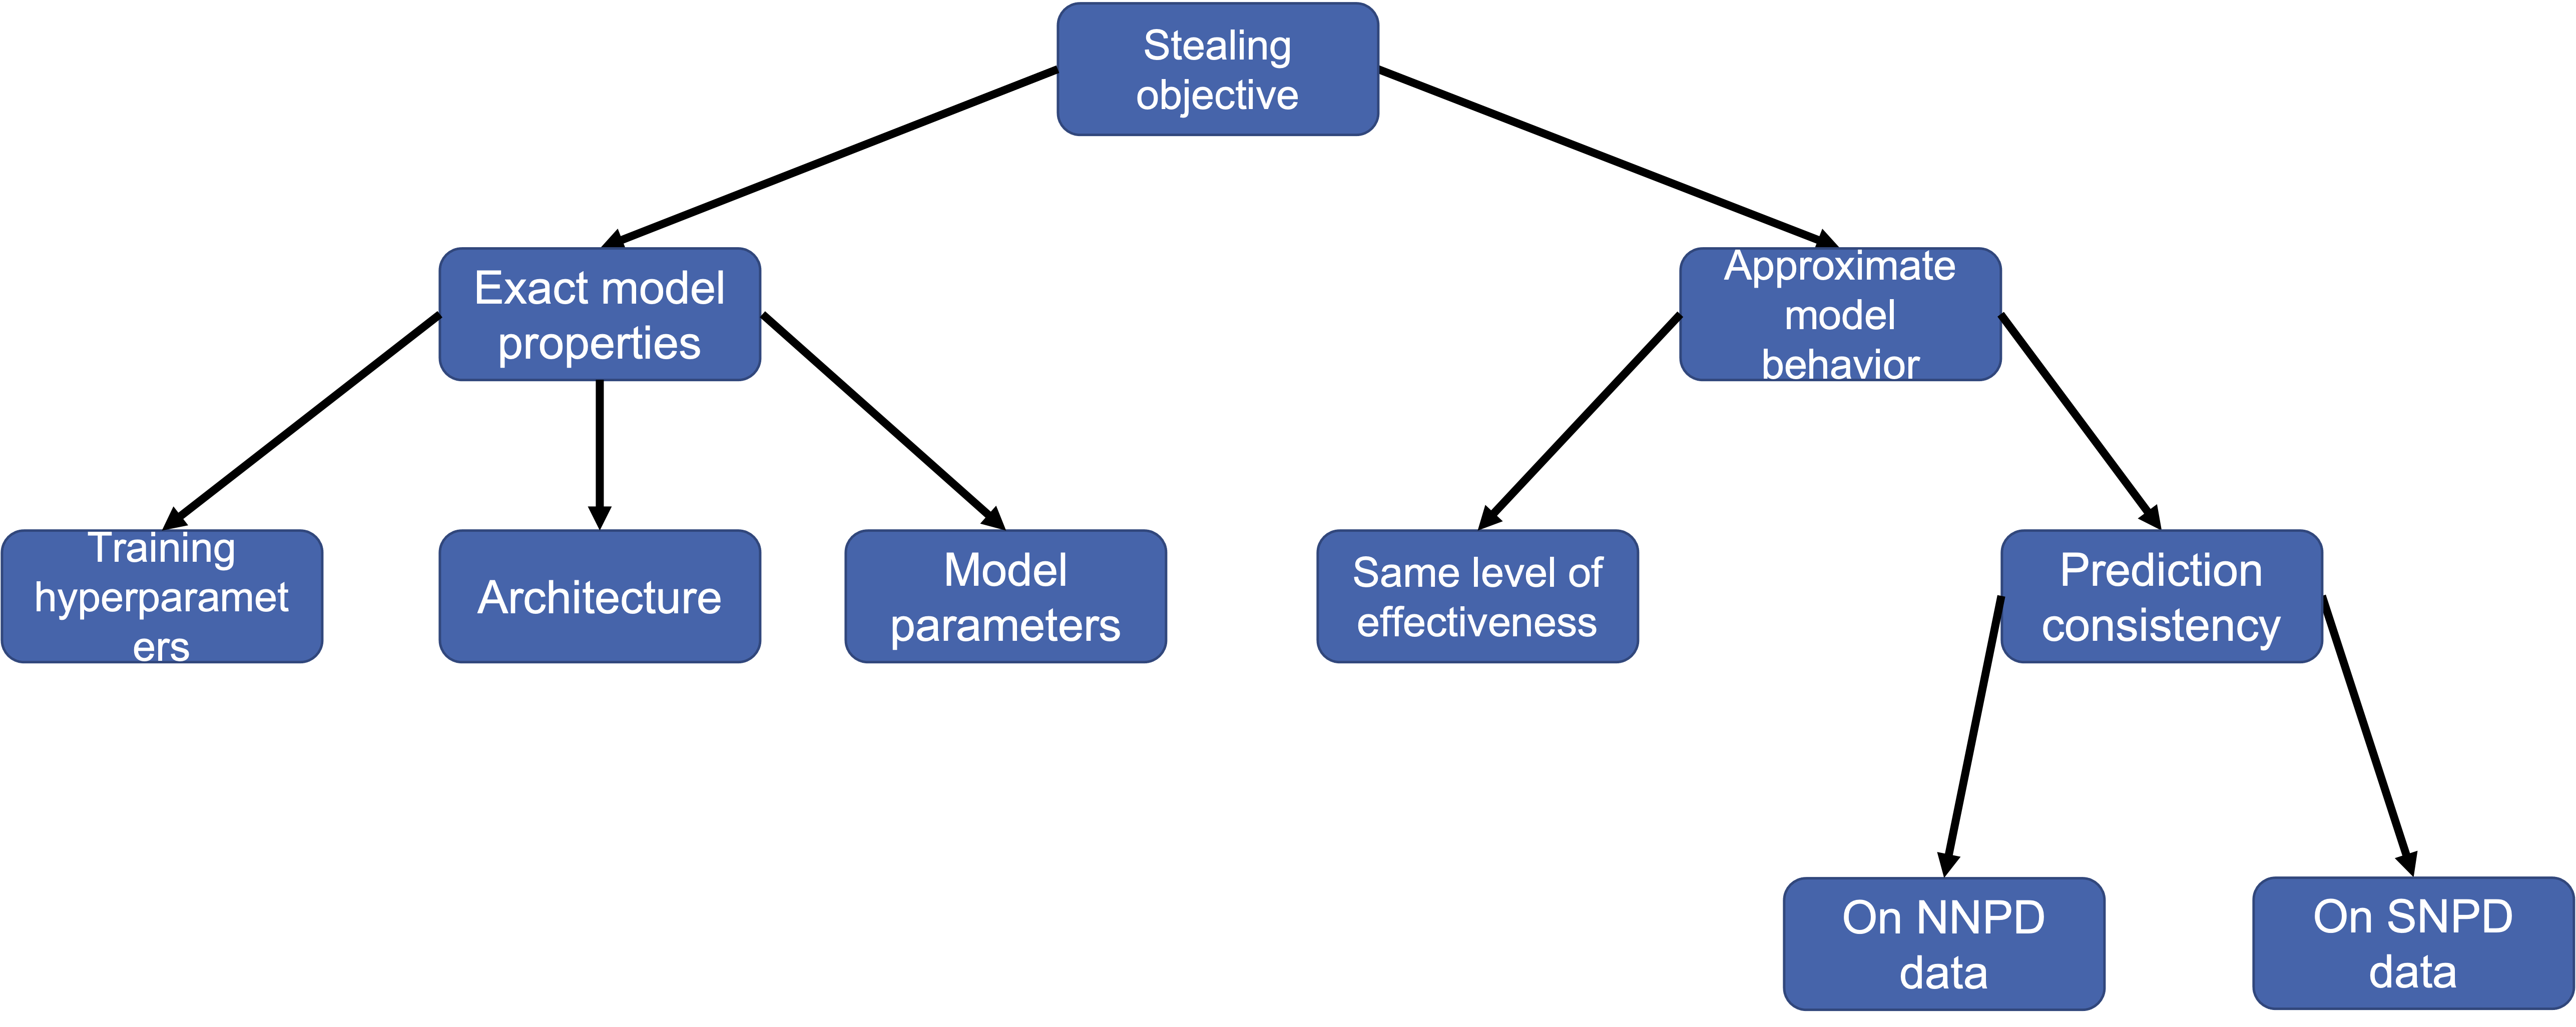
\includegraphics[width=.9\linewidth]{images/MS_Taxonomy.png}
  \caption[Model Stealing Taxonomy]{Taxonomy of Model Stealing Attacks by \cite{oliynyk2022know}}
  \label{fig:ModelStealing:Taxonomy}
\end{figure}


\subsection{Model Stealing Defenses}
\label{sec:ModelStealing:Defenses}
Because of the detrimental effect of Model Stealing Attacks, many defenses have been proposed to protect against them. Defenses can be categorized into proactive and
reactive defenses. While proactive defenses actively aim to prevent or at least complicate Model Stealing Attacks, reactive approaches purely aim to detect them.

\subsubsection{Reactive Model Stealing Defenses (Detection)}
\label{sec:ModelStealing:Defenses:Detection}
Reactive Model Stealing Defenses solely aim to detect Model Stealing Attacks, not prevent them from happening. So far there exist Model Stealing Detection Approaches which
rely either on Watermarking or on Monitoring. Watermarking is a way to prove ownership of a machine learning model. This is usually achieved by \enquote{hiding} information
in the model which can only be restored by the original owner. A watermark can be a predefined prediction value for outlier samples which are unlikely to be part of the thief
dataset. Watermarking can be applied during training \cite{zhang2018protecting} or afterwards \cite{szyller2021dawn}. Monitoring is a way to detect Model Stealing Attacks by
investigating the queries that a user made to the target model. Kesarwani et al. \cite{kesarwani2018model} proposed a method that estimates the relative amount of the data space that a user has
covered with his queries. Based on this metric they can infer the status of a possible extraction attack. Another approach named PRADA \cite{juuti2019prada} analyses the distribution of the
samples that a user has queried so far. They assume that the distance between queries of a benign user follows a normal distribution and any user whose query distances are not normally
distributed is considered to be an attacker. \par

\begin{figure} [ht]
    \centering
    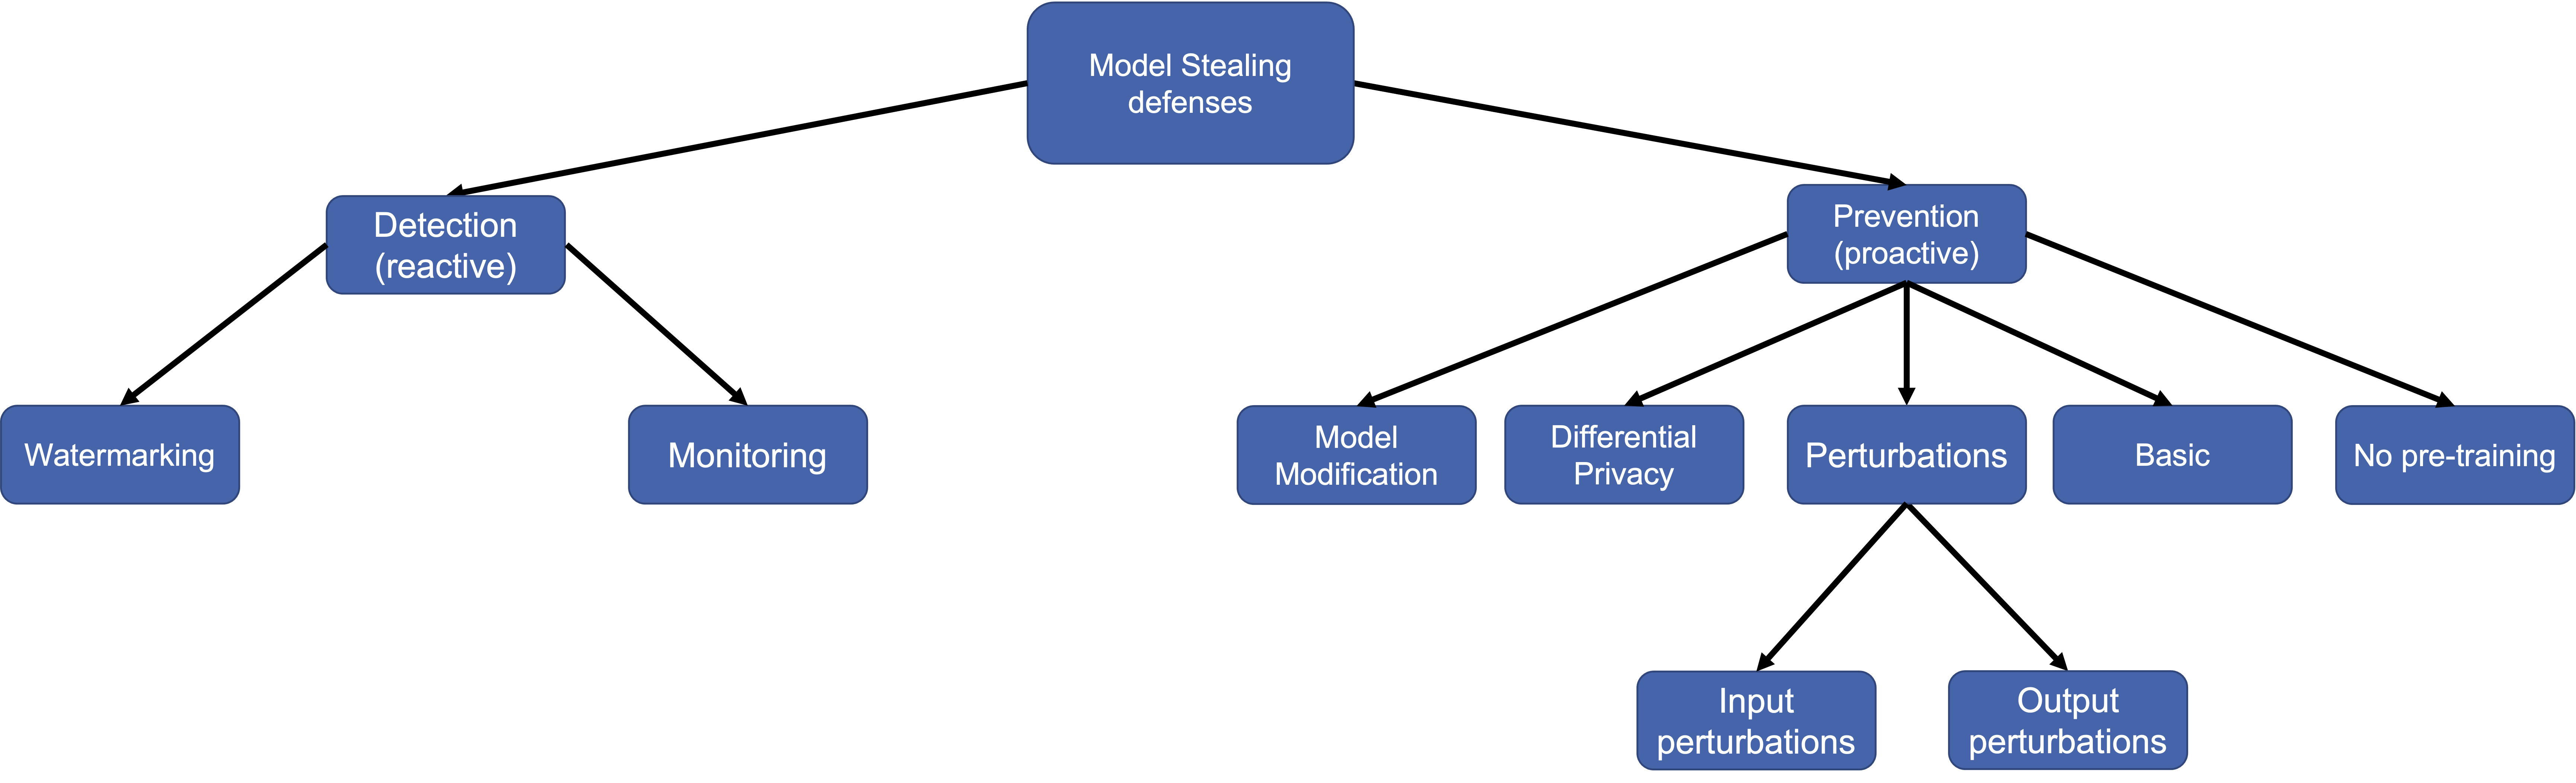
\includegraphics[width=.9\linewidth]{images/MS_defenses_Taxonomy.png}
    \caption[Model Stealing Defenses Taxonomy]{Taxonomy of Model Stealing Defenses by \cite{oliynyk2022know}}
    \label{fig:ModelStealingDefenses:Taxonomy}
  \end{figure}

\subsubsection{Proactive Model Stealing Defenses (Prevention)}
\label{sec:ModelStealing:Defenses:Prevention}
Proactive Model Stealing Defenses aim to complicate or prevent Model Stealing Attacks from happening. It is important to note that the success of a Model Stealing attack is not binary,
compared to breaking into a house for example. Model Stealing Attacks will always be successful to some degree, but their success mainly depends on the accuracy that the substitute model
can achieve (or the achieved model agreement in case the attacker tries to optimize for that). So the quality of a Proactive Model Stealing Defense should be measured by how much it can 
decrease the accuracy of the substitute model compared to a Model Stealing Attack with no defense. A key challenge in developing Proactive Model Stealing Defenses is that, on one hand,
it should be complicated to extract the target model while on the other hand the user experience of benign users should not be affected. \par
Early on, a few basic approaches against Model Stealing Attacks were proposed. These include training several models and randomly choosing the output of one of them 
\cite{alabdulmohsin2014adding}. An even simpler albeit effective approach is to output only the predicted label instead of the vector of output probabilities \cite{tramer2016stealing}.
A downside to this is that a benign user loses a lot of information about the output and the model is less interpretable. Another approach that is similar in complexity is to renounce
using pre-trained models \cite{atli2020extraction} and instead train the target model from scratch. \par
In order to prevent Model Stealing Attacks, researchers have proposed to use data perturbation. One can either choose to perturb the data that is fed to the target model or its prediction.
Input perturbation can for example be performed by adding noise to unimportant pixels determined via Gradient Class Activation Maps \cite{guiga2020neural}. To perform output perturbation,
the developer of the target model can either use Maximizing Angular Deviation (\gls{mad}) \cite{orekondy2019prediction} or flip a few labels to obfuscate the model's decision boundary
\cite{shi2017evasion}. \par
Furthermore, a few approaches have been proposed that bring Differential Privacy into the Model Stealing domain. Differential Privacy is a way to protect the privacy of a dataset so that 
it is impossible for an adversary to determine if a particular individual is part of the dataset. One of these approaches was proposed by Zheng et al. \cite{zheng2019bdpl} who add a so-
called \enquote{Boundary Differential Privacy Layer} to the target model. \par
A final type of Proactive Model Stealing Defense is to modify the target model's architecture. Approaches falling into this category add redundant layers to the target model 
\cite{chabanne2020protection}, propose novel model layers \cite{xu2018deepobfuscation} or increase model sensitivity \cite{szentannai2020preventing}.

%% LaTeX2e class for student theses
%% sections/evaluation.tex
%% 
%% Karlsruhe Institute of Technology
%% Institute for Program Structures and Data Organization
%% Chair for Software Design and Quality (SDQ)
%%
%% Dr.-Ing. Erik Burger
%% burger@kit.edu
%%
%% Version 1.3.6, 2022-09-28

\chapter{Related Work}
\label{ch:Related_work}
We present related work for this thesis in this chapter. First, we will outline the basic idea of each active learning strategy we
use in our experiments. Next, we give an overview of the continual learning approaches we use. Finally, we will introduce ActiveThief, the
model stealing framework we extend in this thesis.


\section{Active Learning}
\label{sec:Related_work:Active_Learning}
In this section, we will present the active learning strategies we will use in our experiments. These are least confidence
(\gls{lc}), CoreSet, bayesian active learning by disagreement (\gls{bald}), batch active learning by diverse gradient embeddings (\gls{badge}), and 
variational adversarial active learning (\gls{vaal}). While we aim to give a detailed explanation of these approaches, we refer to the
original papers for any further details. \par

\subsection{Least Confidence}
\label{sec:Related_work:Active_Learning:Least_Confidence}
Least confidence (\gls{lc}) is one of the earlier approaches to active learning. \gls{lc} is an uncertainty-based \gls{al}
approach proposed by Lewis et al. \cite{lewis1995sequential} in 1994. The idea behind \gls{lc} is that the next points to label should be the 
ones with the lowest prediction probability. More formally, the data queried will be the following:
\begin{equation}
    \argmin_{x \in U} \max_{y \in Y} p(y|x)
\end{equation}
where $U$ is the set of unlabeled data points and $Y$ is the set of possible labels. \par

\subsection{CoreSet}
\label{sec:Related_work:Active_Learning:CoreSet}
CoreSet, sometimes named $k$-center strategy, is an active learning method specifically proposed for \glspl{cnn} \cite{sener2017active}.
Sener and Savarese redefine the pool-based active learning problem (for the original definition, see 
section \ref{sec:PoolBasedActiveLearning}) as 
\begin{equation}
    \min_{s^1 \subseteq U: |s^1| \leq b } \abs{\frac{1}{|L \cup U|} \sum_{x_i,y_i \in L \cup U} \mathcal{L}(x_i,y_i;L \cup s^1) - \frac{1}{|L \cup s^1|} 
    \sum_{j \in L \cup s^1} \mathcal{L}(x_j,y_j,L \cup s^1)}, 
\end{equation}
where $L$ is the labeled set, $U$ is the unlabeled set and $b$ is the batch size.
Informally, we select the data points to add to the labeled pool, which ensure the best loss approximation
of a model trained on the labeled set compared to a model trained on the whole dataset. The authors assume zero training error, which
simplifies the equation above to
\begin{equation}
    \frac{1}{|L \cup U|} \sum_{x_i,y_i \in L \cup U} \mathcal{L}(x_i,y_i;L \cup s^1)
\end{equation}
Sener and Savarese show that minimizing this equation is equivalent to solving the $k$-Center problem \cite{wolf2011facility}, i.e.
\begin{equation}
    \min_{s^1: |s^1| \leq b} \max_i \min_{j \in s^1 \cup L}  \Delta (x_i,x_j)
\end{equation}
This problem is NP-hard but can be solved by the 2-OPT greedy algorithm presented in algorithm \ref{alg:kCenterGreedy}.
\begin{algorithm}
    \caption{$k$-Center-Greedy} \label{alg:kCenterGreedy}
    \begin{algorithmic}
        \Require data $x_i$, labeled pool $L$ and budget $b$
        \State Initialize s = $L$
        \Repeat
        \State $u = \argmax_{x_i \in U \setminus s} \min_{x_j \in s} \Delta(x_i,x_j)$
        \State $s = s \cup \{u\}$
        \Until{$|s| = b$}
        \return $s \setminus L$
    \end{algorithmic}
\end{algorithm}
The authors propose a more sophisticated algorithm that performs marginally better than the greedy solution but is approximately 
four times slower. Therefore, we omit the proposed algorithm in this section.

\subsection{Bayesian Active Learning by Disagreement}
\label{sec:Related_work:Active_Learning:BALD}
Bayesian active learning by disagreement (\gls{bald}) is an uncertainty-based \gls{al} strategy proposed by Houlsby et al. 
\cite{houlsby2011bayesian}. \gls{bald} uses Shannon's entropy \cite{cover1991information} to determine a model's prediction uncertainty for a given
unlabeled data point. More precisely, a learner using \gls{bald} will query the sample(s) fulfilling the following condition
\begin{equation}
    \argmax_{x \in U} H[y \mid x, L] - \mathbb{E}_{\theta \sim p(\theta \mid L)} [H[y \mid x, \theta]]
\end{equation}
where $H$ is the entropy, $U$ is the set of unlabeled data points, and $L$ is the set of labeled data points.
Informally, \gls{bald} selects those data points with the largest gap between the model's actual prediction uncertainty and the model's expected
prediction uncertainty. Since the expected prediction uncertainty cannot be computed given that the parameter distribution conditioned on the
previously observed data is unknown, \gls{bald} uses Monte Carlo sampling to approximate the expected prediction uncertainty. For neural networks, Monte
Carlo dropout \cite{gal2016dropout} can be applied.

\subsection{Batch Active Learning by Diverse Gradient Embeddings}
\label{sec:Related_work:Active_Learning:BADGE}
Batch active learning by diverse gradient embeddings (\gls{badge}) \cite{ash2019deep} is a batch active learning strategy that combines both model uncertainty
and batch diversity to select the next batch of data points to label. The authors were inspired to develop \gls{badge} by the observation that diversity-based
active learning strategies perform well in the first few iterations, while uncertainty-based approaches perform well in the later stages of active learning.
\gls{badge} therefore incorporates both uncertainty and diversity in its selection strategy. Furthermore, \gls{badge} uses the
gradient with respect to the output layer as a measure of model uncertainty, similar to the ideas of Zhang et al. \cite{zhang2017active} and Settles et al. \cite{settles2007multiple}.
Since \gls{badge} works on unlabeled data points, the gradient cannot be computed analytically because the label is unknown. Therefore, \gls{badge} uses the hypothetical
label $\hat{y}(x)$ as a proxy for the true label and computes the gradient of the cross-entropy loss on the hypothetical label as an approximation of the
actual gradient. To incorporate diversity, \gls{badge} uses $k$-means++ initialization \cite{arthur2007k} for the gradient embeddings to sample the next batch of data
points to label. The authors demonstrate \gls{badge}'s agnosticism towards model architecture, training hyperparameters, and datasets in mutliple experiments.
\begin{algorithm}
    \caption{\gls{badge}} \label{alg:Badge}
    \begin{algorithmic}[1]
        \Require Neural network $f(x;\theta)$, unlabeled pool $U$, labeled pool $L=\emptyset$, number of iterations $T$, bath size $b$
        \State Labeled dataset $L \leftarrow k$ random samples from $U$ together with their labels
        \State Train initial model $\theta_1$ on $L$
        \For{$t = 1,2,\ldots,T$}
            \State For all examples $x$ in $U \setminus L$:
            \begin{enumerate}[leftmargin=0.8in]
                \item Compute its hypothetical label $\hat{y}(x) = h_{\theta_t}(x)$
                \item Compute gradient embeddings $g_x = \frac{\partial}{\partial \theta_{out}} \mathcal{L}_{\text{CE}}(f(x;\theta_t),\hat{y}(x))$, where
                $\theta_{out}$ refers to parameters of the final (output) layer.
            \end{enumerate}
            \State Compute $S_t$, a subset of $U \setminus L$ of size $b$, using the $k$-MEANS++ seeding algorithm on {\color{white} 123}$\{ g_x: x \in U
            \setminus L\}$ and query for their labels.
            \State Update labeled pool $L \leftarrow L \cup S_t$
            \State Train new model $\theta_{t+1}$ on $L$
        \EndFor
        \return Final model $\theta_T$
    \end{algorithmic}
\end{algorithm}

\subsection{Variational Adversarial Active Learning}
\label{sec:Related_work:Active_Learning:VAAL}
Variational adversarial active learning (\gls{vaal}) is a representation-based active learning strategy proposed by Sinha et al. \cite{sinha2019variational}. 
\gls{vaal} uses a $\beta$-variational autoencoder (\gls{vae}) \cite{higgins2017beta} and a discriminator to select the most informative samples to query.
Thereby, the encoder learns a low-dimensional space for the distribution of the labeled and the unlabeled data reconstructed by the decoder. 
The discriminator is trained to distinguish between the labeled and the unlabeled data and given the encoder's latent representation of a data point as an
input. We provide a visual summary of the approach in figure \ref{fig:VAAL}. \par
More formally, the encoder learns the distribution of $X_U$ and $X_L$ where $X_U$ is the unlabeled pool and $(X_L, Y_L)$ is the labeled pool. The encoder
aims to minimize the \gls{kl} divergence \cite{goldberger2004hierarchical} between the reconstructed distribution $q_\Phi (z_L | x_L)$ and
the real distribution $p(z)$ of the labeled data, which we assume to be a unit Gaussian. Simultaneously, the encoder aims to minimize the \gls{kl} divergence
between $q_\Phi (z_U | x_U)$ and $p(z)$. This results in the following objective function for the \gls{vae}:
\begin{equation}
    \mathcal{L}^{trd}_{VAE} = \mathbb{E}[\log p_\theta (x_L | z_L)] - \beta D_{KL} (q_\Phi (z_L | x_L) || p(z)) + \mathbb{E}[\log p_\theta (x_U | z_U)] - \beta D_{KL} (q_\Phi (z_U | x_U) || p(z))
\end{equation}
where $p_\theta$ and $q_\Phi$ are the decoder and the encoder. The discriminator $D$ is trained to distinguish between the latent space representation
of labeled and unlabeled data. Additionally, the \gls{vae} is trained to make samples from the labeled and
unlabeled data indistinguishable to complicate the classification of the discriminator. The adversarial objective function for the discriminator is given by:
\begin{equation}
    \mathcal{L}^{adv}_{VAE} = - \mathbb{E}[\log(D(q_\theta (z_L | x_L)))] - \mathbb{E}[\log(D(q_\theta(z_U | x_U)))].
\end{equation}
Both equations above result in the following final loss function for the \gls{vae}:
\begin{equation}
    \mathcal{L}_{VAE} = \lambda_1 \mathcal{L}^{trd}_{VAE} + \lambda_2 \mathcal{L}^{adv}_{VAE}
\end{equation}
where $\lambda_1$ and $\lambda_2$ are hyperparameters, trading off between adversarial training and optimal reconstruction. \par
The discriminator loss is given by:
\begin{equation}
    \mathcal{L}_D = - \mathbb{E}[\log(D(q_\theta (z_L | x_L)))] - \mathbb{E}[\log (1- D(q_\theta (z_U | x_U)))].
\end{equation}
To query a batch of samples of size $b$, the \gls{vae} and discriminator are first trained on the entire pool of labeled and unlabeled data for a
pre-specified number of epochs $e$. The samples chosen by \gls{vaal} are the ones where the discriminator is most confident about their belonging to the unlabeled
pool or, in other words, least confident about their belonging to the labeled pool.
\begin{figure} [ht]
    \centering
    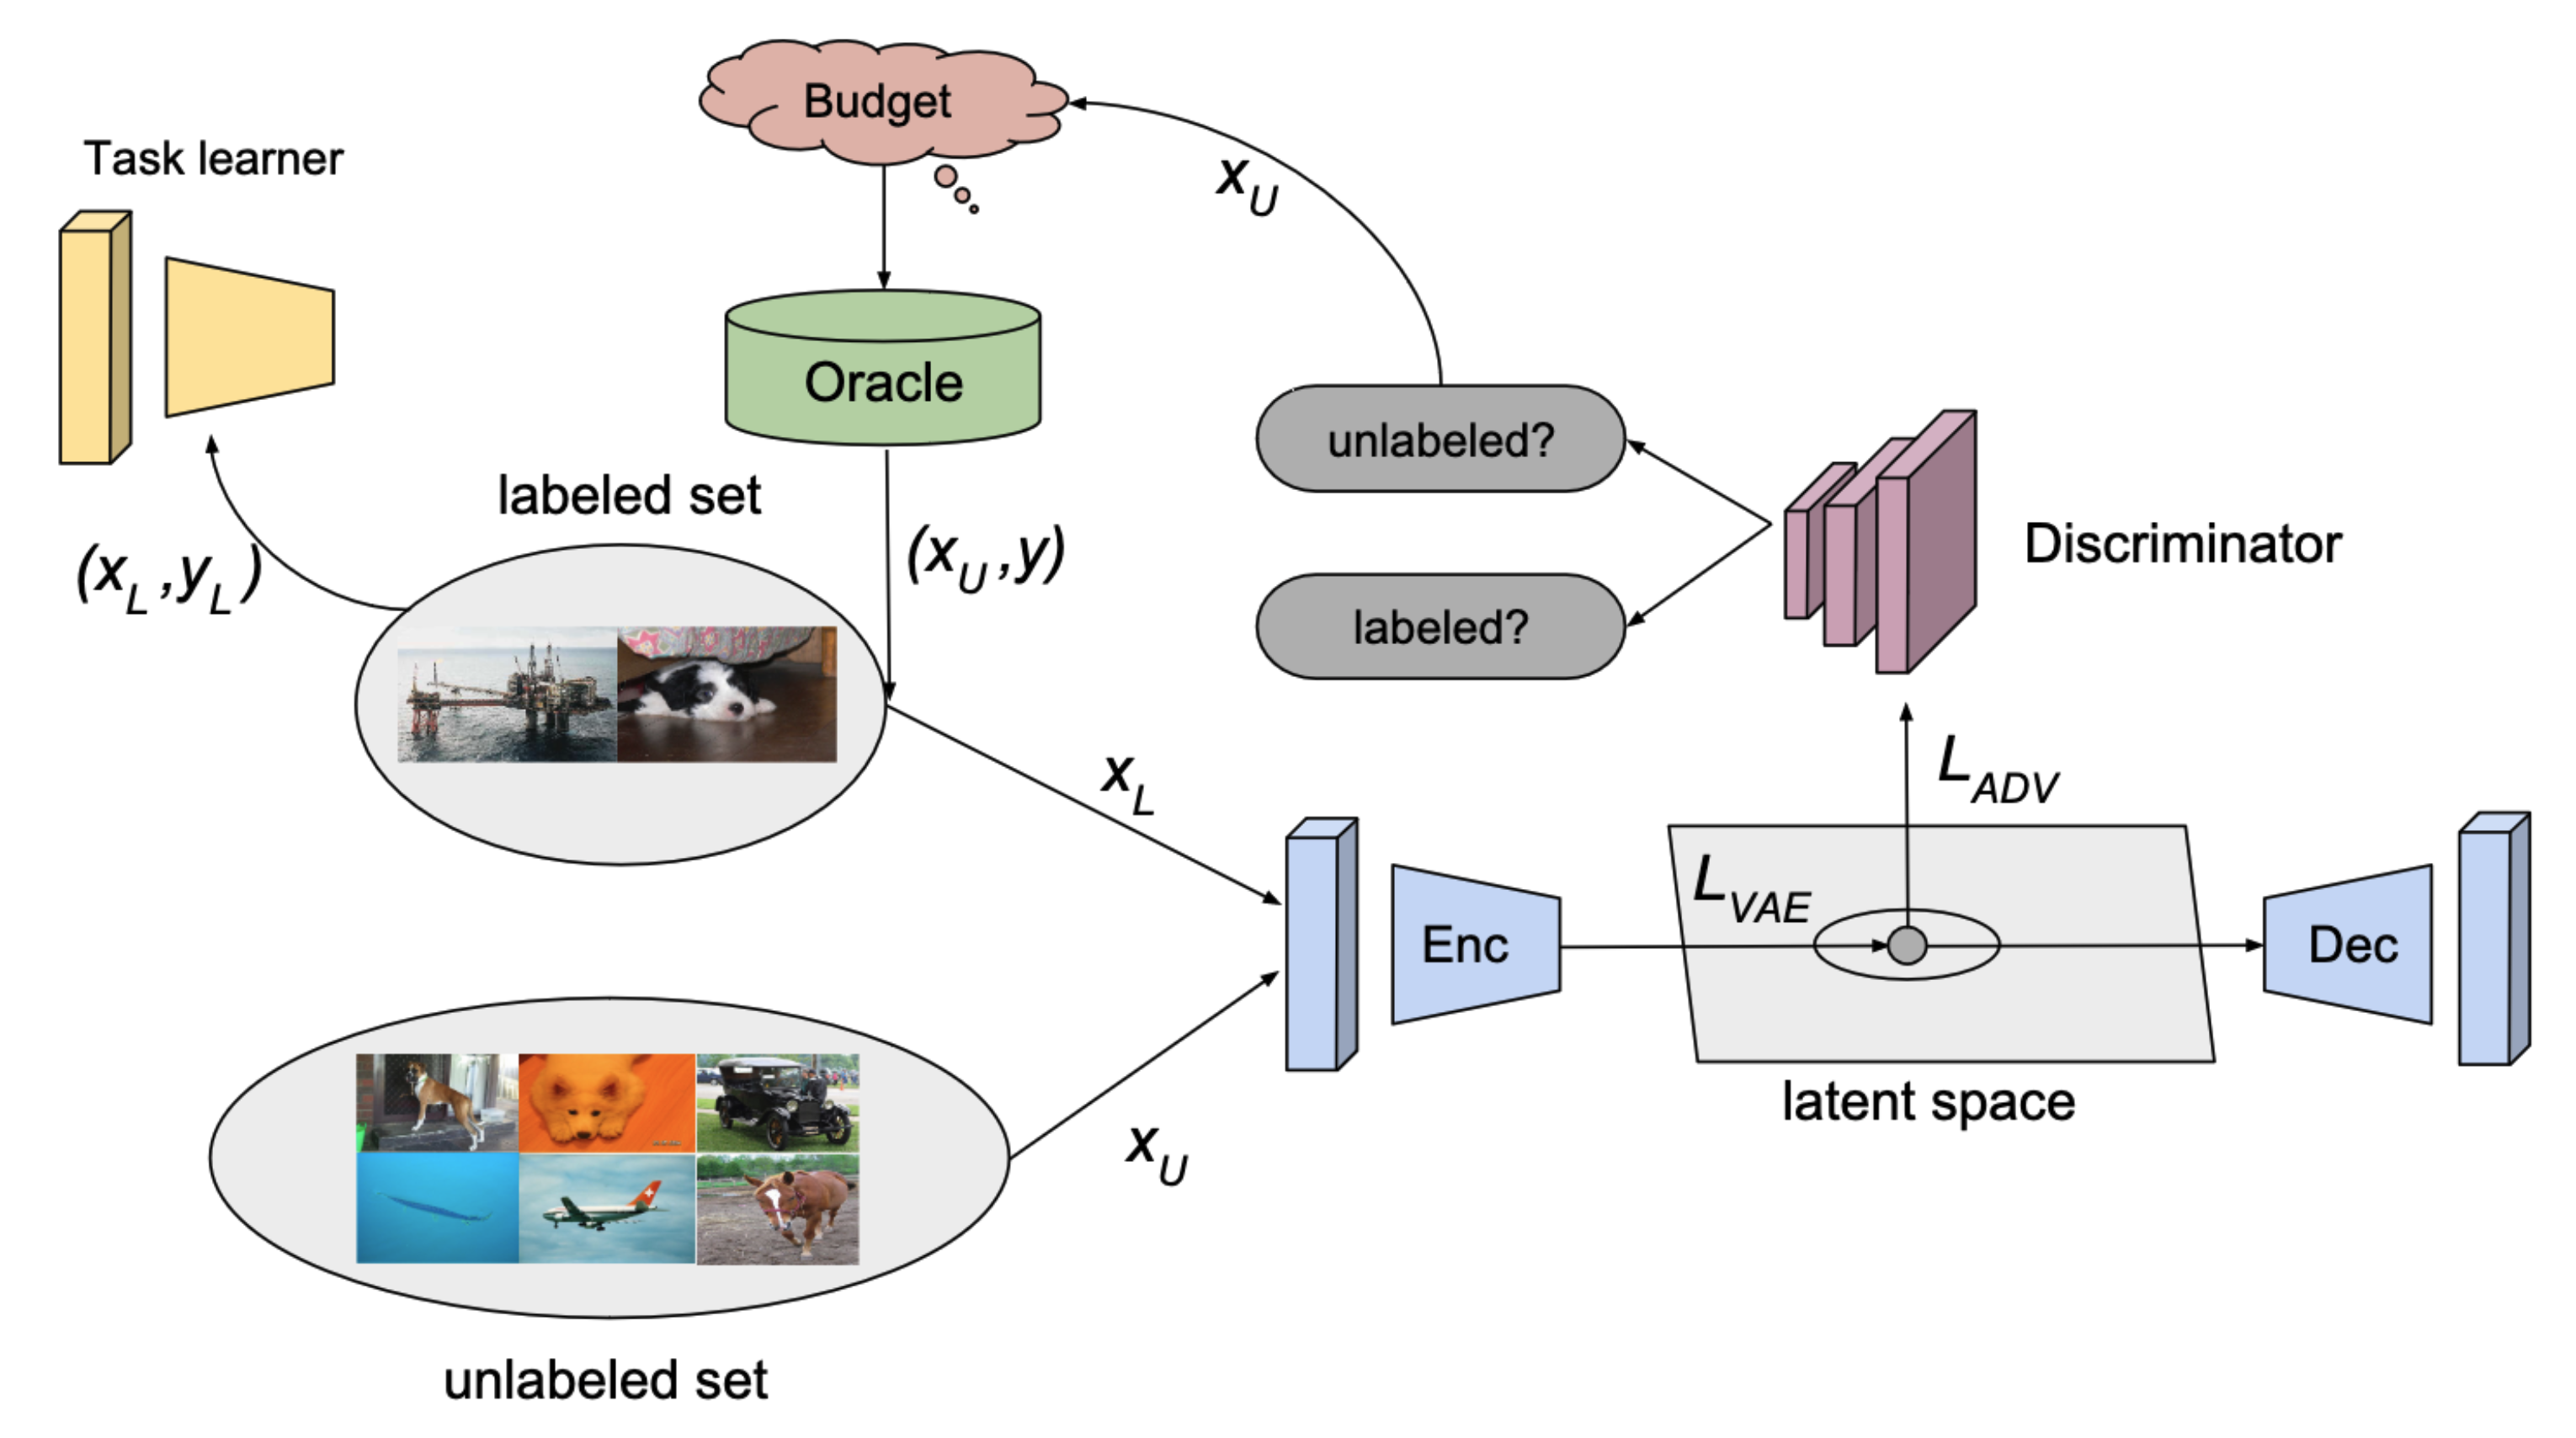
\includegraphics[width=.8\linewidth]{images/Vaal_idea.png}
    \caption[Visualization of \gls{vaal}]{Illustration of the idea of \gls{vaal} taken from the paper of Sinha et al. \cite{sinha2019variational}.}
    \label{fig:VAAL}
\end{figure}


\section{Continual Learning}
\label{sec:Related_work:Continual_Learning}
In this section, we will present the continual learning algorithms used in our experiments. These are elastic weight
consolidation (\gls{ewc}) \cite{kirkpatrick2017overcoming}, memory aware synapses (\gls{mas}), asymmetric loss approximation by single-side overestimation
(\gls{alasso}), incremental moment matching (\gls{imm}) and averaged gradient episodic memory (\gls{a-gem}) \cite{lopez2017gradient}. While we aim to give
a detailed explanation of these approaches, we refer to the original papers for any further details. \par

\subsection{Elastic Weight Consolidation}
\label{sec:Related_work:Continual_Learning:EWC}
Elastic weight consolidation (\gls{ewc}) \cite{kirkpatrick2017overcoming} is a structural regularization approach proposed by Kirkpatrick et al.
\gls{ewc} was the first approach aiming to overcome catastrophic forgetting by regularizing model parameters. This is done by adding a regularization
term to the loss function, which resembles $l_2$-regularization. The regularization loss is introduced to constrain important parameters for
task $N-1$ to stay close to their previous values when training on task $N$. To come up with an importance measure for the parameters,
Kirkpatrick et al. view neural network training from a probabilistic perspective, modeling the weight distribution using the Bayes rule:
\begin{equation}
    p(\theta \mid D) = \frac{p(D \mid \theta) \cdot p(\theta)}{p(D)}.
\end{equation}
When applying the logarithm, this can be rewritten as
\begin{equation}
    \log p(\theta \mid D) = \log p(D \mid \theta) + \log p(\theta) - \log p(D)
\end{equation}
and when splitting the whole dataset $D$ into $D_{1:N-1}$ and $D_N$, this equates to
\begin{equation}
    \log p(\theta \mid D) = \log p(D_N \mid \theta) + \log p(\theta \mid D_{1:N-1}) - \log p(D_N),
\end{equation}
meaning that only the term $\log p(\theta \mid D_{1:N-1})$ is dependent on the previous tasks. Therefore, it must contain the full information 
about all previous tasks. Since $\log p(\theta \mid D_{1:N-1})$ cannot be computed, Kirkpatrick et al. approximate it using Laplace's approximation
\cite{mackay2003information}, obtaining a Gaussian distribution with mean of $\theta^*_{1:N-1}$ and covariance matrix $[\mathbb{I}_{D_{1:N-1}}]^{-1}$,
where
\begin{equation}
    \mathbb{I}_{D_{1:N-1}} = \mathbb{E} [- \frac{\partial^2 \theta (\log (p(\theta \mid D_{1:N-1})))}{\partial^2 \theta} \mid_{\theta^*_{D_{1:N-1}}}]
\end{equation} 
which is the Fisher information matrix (\gls{fim}) as shown by Aich \cite{aich2021elastic}. A large value of $F_i$, the $i$-th diagonal of the \gls{fim},
indicates a small variance in the posterior distribution of the parameter, meaning that it is important for previous tasks. Therefore, $F_i$, is used as an
importance measure for the $i$-th parameter. To conclude, the loss function for a Task $N$ is altered to
\begin{equation}
    \mathcal{L}(\theta) = \mathcal{L}_B(\theta) + \sum_i \frac{\lambda}{2} F_i \cdot (\theta_i - \theta^*_{N-1,i})^2,
\end{equation}
where $\mathcal{L}_B(\theta)$ is the loss function of the model on the current task (e.g. cross-entropy loss), $\theta_i$ is the $i$-th parameter of the model,
and $\theta^*_{N-1,i}$ is the $i$-th parameter of the model trained on the previous task. The hyperparameter $\lambda$ is used to trade-off between
learning new tasks and retaining knowledge of previous tasks.

\subsection{Memory Aware Synapses}
\label{sec:Related_work:Continual_Learning:MAS}
Memory aware synapses (\gls{mas}), like \gls{ewc}, is a structural regularization method proposed by Aljundi et al. \cite{aljundi2018memory}. 
In line with \gls{ewc}, \gls{mas} aims to prevent catastrophic forgetting by regularizing model parameters. The main difference between \gls{ewc} and
\gls{mas} the composition of their importance measure. While \gls{ewc} relies on Fisher information to compute parameter importances, \gls{mas} uses
gradient magnitude to estimate the importance of a parameter for previous tasks. To derive the importance measure, the authors first observe that the
effect of small changes to the network parameters on the prediction can be approximated as follows
\begin{equation}
    f(x_k; \theta + \delta) - f(x_k; \theta) \approx = \sum_i g_i(x_k) \cdot \delta_i
\end{equation}
where $g_i(x_k) = \frac{\partial(f(x_k;\theta))}{\partial \theta_i}$  is the gradient with respect to parameter $\theta_i$ when evaluating the model at
input $x_k$. Since most classification models, like neural networks, for example, have a multi-dimensional output Aljundi et al. propose to use the gradient
of the squared $l_2$-Norm in this setting, i.e. $g_i(x_k) =  \frac{\partial[l^2_2(f(x_k;\theta))]}{\partial \theta_i}$. With the approximation given by the
equation above, the authors claim that the importance of a parameter $\theta_i$ can be computed as
\begin{equation}
    \omega_i = \frac{1}{n} \sum_{k=1}^n \lVert g_i(x_k) \rVert
\end{equation}
where $n$ is the number of data points observed so far. The advantage of computing the importance measure as stated above is that it can be updated when-
ever a new data point is observed. However, it is more efficient to update the $\omega$s batch-wise. The overall loss function for a task $N$ is
then altered for the standard setting as follows
\begin{equation}
    \mathcal{L}(\theta) = \mathcal{L}_N(\theta) + \lambda \sum_i \omega_i \cdot (\theta_i - \theta^*_{N-1,i})^2
\end{equation}
where $\lambda$ again is the hyperparameter used to trade-off between learning new tasks and retaining the knowledge of previous tasks.

\subsection{Asymmetric Loss Approximation by Single-Side Overestimation}
\label{sec:Related_work:Continual_Learning:ALASSO}
Asymmetric loss approximation by single-side overestimation (\gls{alasso}) is a structural regularization method proposed by Park et al. \cite{park2019continual}.
\gls{alasso} is an extension of \gls{si} proposed by Zenke et al. \cite{zenke2017continual}. Park et al. claim that \gls{alasso} \enquote{mitigates the limitations of SI}.
The main observation they made about \gls{si} is that it underestimates the true loss on the unobserved side of the loss
function because it assumes that the loss function is symmetric. Park et al. first show that this assumption is not always correct through empirical observation
and then present a new approach to approximate the loss function on the unobserved side. We present the fundamental observation and idea of \gls{alasso} in figure
\ref{fig:Alasso}. Since \gls{alasso} extends the \gls{si} framework, we strongly recommend the reader familiarize themselves with \gls{si} before
trying to understand \gls{alasso}. In the following, we will assume that the reader is familiar with \gls{si} and only explain the extension that \gls{alasso}
brings to \gls{si}. \par
Since \gls{alasso} is a structural regularization method like \gls{mas} and \gls{ewc}, it alters the loss function as follows
% Total loss equation
\begin{equation}
    \tilde{\mathcal{L}}^N = \mathcal{L}^N + c \sum_k \mathcal{L}_s^{N-1}(\theta_k,a),
\end{equation}
meaning that it adds a surrogate loss to the loss function, which is controlled via the hyperparameter $c$. To understand how the surrogate loss is composed
\gls{alasso} first introduces $\alpha(\theta_k)$, which determines for a model parameter if it is on the observed or unobserved side of the loss function.
$\alpha(\theta_k)$ is defined as follows
% Alpha equation
\begin{equation}
    \alpha(\theta_k) = (\theta_k - \hat{\theta}^N_k) (\hat{\theta}^{N-1}_k - \hat{\theta}^N_k)
\end{equation}
The surrogate loss $\mathcal{L}^N_s(\theta_k,a)$ is then defined as follows
% Loss estimation equation
\begin{equation}
    \mathcal{L}_s^n(\theta_k,a) = \begin{cases} \hat{\Omega}^N_k (\theta_k - \hat{\theta}_k)^2 & \text{if} \alpha(\theta_k) > 0 \\
    (a \hat{\Omega}^N_k + \epsilon)(\theta_k - \hat{\theta}_k)^2 & \text{if} \alpha(\theta_k) \leq 0 \end{cases}.
\end{equation}
Again, the variable $a (>1)$ is a hyperparameter used to control the amount of overestimation if the parameter is on the unobserved side of the loss function.
The constant $\epsilon$ is used to make sure that the loss on the unobserved side is always overestimated, i.e., $(a \hat{\Omega}^N_k + \epsilon) > \hat{\Omega}^N_k$.
The second contribution of \gls{alasso} is its derivation of the optimal coefficient $\hat{\Omega}^N_k$ for the approximation of the loss function on the \textit{observed}
side. According to Park et al., $\hat{\Omega}^N_k$ is determined by the following equation
% Omega equation
\begin{equation} \label{eq:ALASSO_Omega}
    \hat{\Omega}^N_k = \frac{\omega^N_k + \omega^{1:N-1}_k}{(\hat{\theta}^N_k - \hat{\theta}^{N-1}_k)^2},
\end{equation}
where $\omega^N_k$ and $\omega^{1:N-1}_k$ are given by
% Small Omega equation
\begin{gather} \label{eq:ALASSO_Small_Omega}
    \omega^N_k = \mathcal{L}^N(\hat{\theta}^{N-1}_k) - \mathcal{L}^N(\hat{\theta}^N_k) \\
    \omega^{1:N-1}_k = -c\mathcal{L}^{N-1}_s(\hat{\theta}^N_k,a)
\end{gather}
Because of the ambiguous influence of the hyperparameters $c$ and $a$ to the approximation of the loss function, the authors of \gls{alasso} propose to decouple them. More
precisely, they suggest using $c'$ and $a'$ instead of $c$ and $a$ in equation 3.23.

\begin{figure} [ht]
    \centering
    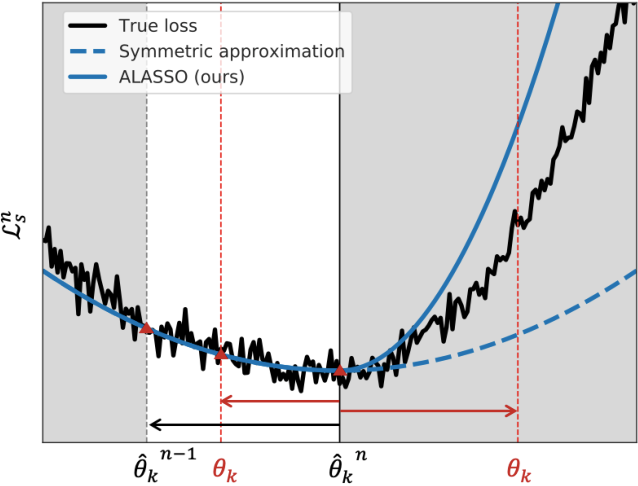
\includegraphics[width=.5\linewidth]{images/Alasso_Idea.png}
    \caption[Visualization of \gls{alasso}]{Illustration of the idea of \gls{alasso} taken from the paper of Park et al. \cite{park2019continual}. The authors of \gls{alasso}
     state that, \gls{si}
    underestimates the unobserved side of the loss function and hence a better approximation of the loss function is achieved by overestimating it.}
    \label{fig:Alasso}
\end{figure}

\subsection{Incremental Moment Matching}
\label{sec:Related_work:Continual_Learning:IMM}
Incremental moment matching (\gls{imm}) is a structural regularization approach, proposed by Lee et al. \cite{lee2017overcoming}.
\gls{imm} deviates from approaches like \gls{mas} and \gls{ewc} in that it should not be viewed as a single method but rather a framework of multiple methods,
many of which can be combined. The main idea of \gls{imm} is to match the first and second moments of the posterior distribution $p(\theta \mid D_{1:N})$ of the model 
parameters given all tasks up to the current one. As in \gls{ewc}, the posterior distribution cannot be computed. Therefore, it is approximated via a Gaussian distribution which
we call $q_{1:N}$. The first approach to matching these moments is called mean-based incremental moment matching, also known as mean-\gls{imm}. The weight
update of mean-\gls{imm} is the analytical solution of the problem to minimize the weighted sum of \gls{kl} divergences between each $q_i$ and $q_{1:N}$
\cite{goldberger2004hierarchical}, i.e. the solution to
\begin{equation}
    \argmin_{\mu^*_{1:N},\Sigma^*_{1:N}} \sum_{i=N-k}^N \alpha_i \cdot KL(q_i \mid \mid q_{1:N})
\end{equation}
which is given by
\begin{gather}
    \mu^*_{1:N} = \sum_{i=N-k}^N \alpha_i \cdot \mu_i \\
    \Sigma^*_{1:N} = \sum_{i=N-k}^N \alpha_i (\Sigma_i + (\mu_i - \mu^*_{1:N})(\mu_i - \mu^*_{1:N})^T)
\end{gather}
The $\alpha_i$ are the mixing coefficients that weigh the previous $k$ tasks and have the constraint $\sum_{i=N-k}^N \alpha_i = 1$.  \\
The second approach to matching the moments is called mode-based incremental moment matching, also known as mode-\gls{imm}. mode-\gls{imm}
further incorporates covariance information from previous tasks to match the first and second moments of the posterior distribution. 
The mean and covariance update for mode-\gls{imm} is given by
\begin{gather}
    \mu^*_{1:N} = \sum_{i=N-k}^N \alpha_i \cdot (\sum_{i=N-k}^N \alpha_i \Sigma_i^{-1} \mu_i) \\
    \Sigma^*_{1:N} = (\sum_{i=N-k}^N \alpha_i  \Sigma_i^{-1})^{-1}
\end{gather}
To approximate the covariance matrix, mode-\gls{imm} uses the inverse of the \gls{fim} like \gls{ewc}. Furthermore, the authors assume that
the model parameters are pairwise independent, making the covariance matrix diagonal and therefore save computation. \par
Apart from moment matching methods, \gls{imm} also includes approaches to transfer model parameters from previous tasks. The first approach is called
weight transfer. When using continual learning with weight transfer, the parameters of the previous task are used as initialization for the
current task. This approach is very similar to the term warm start commonly used in active learning. $l_2$-transfer, which is a special form of 
$l_2$-regularization, is the next transfer technique. $l_2$-transfer can be seen as a special form of \gls{ewc} where all the $F_i$s are set to 1. 
With $l_2$ transfer, the loss function is altered to
\begin{equation}
    \log p(y_N \mid X_N, \mu_N) - \lambda \cdot {\lVert \mu_N - \mu_{N-1} \rVert}^2_2
\end{equation}
with $\lambda$ being a hyperparameter. The third transfer technique is \textbf{Drop-transfer}. Drop-transfer
\begin{equation}
    \hat{\mu}_{N,i} = \begin{cases} \mu_{N,i}, & \text{if the }i \text{th node is turned off} \\
    \frac{1}{1-p} \cdot \mu_{N,i} - \frac{p}{1-p} \cdot \mu_{N-1,i}, & \text{otherwise}  \end{cases}
\end{equation}
where $p$ is the dropout ratio. Drop-transfer can be seen as a further regularizer for continual learning, with similar effect to $l_2$-transfer albeit
being orthogonal to it. In algorithm \ref{alg:IMM}, we show the pseudocode for \gls{imm} with weight-transfer and $l_2$-transfer. \par

\begin{algorithm}
    \caption{\gls{imm} with weight-transfer, $l_2$-transfer} \label{alg:IMM}
    \begin{algorithmic}
        \Require data $f\{ (X_1,Y_1),\ldots,(X_N,Y_N)\}$, balancing hyperparameter $\alpha$ with $\sum_{i=1}^k \alpha_i = 1$,
        regularization hyperparameter $\lambda$
        \return $w_{1:N}$
        \State $w_0 \leftarrow $ InitializeNN()
        \For{$i=1:N$}
            \State $w_{i*} \leftarrow w_{i-1}$
            \State Train($w_{i*},X_i,Y_i$) with $L(w_{i*},X_i,Y_i) + \lambda \cdot (\lVert w_{i*} - w_{i-1} \rVert)^2_2$
            \State $m=\max (0,i-k)$
            \If{type is mean-IMM}
            \State $w_{i*} \leftarrow \sum_{t=max(0,i-k)}^i \alpha_t w_{t}$
            \ElsIf{type is mode-IMM}
            \State $F_{i*} \leftarrow$ CalculateFisherMatrix($w_{i*},X_i,Y_i$)
            \State $\Sigma_{1:i} \leftarrow (\sum_{t=max(0,i-k)}^i \alpha_t F_{t*} w_{t*})^{-1}$
            \State $w_{i*} \leftarrow \Sigma_{1:i} \cdot (\sum_{t=max(0,i-k)}^i \alpha_t F_{t*} w_{t*})$
            \EndIf
        \EndFor
    \end{algorithmic}
\end{algorithm}

\subsection{Averaged Gradient Episodic Memory}
\label{sec:Related_work:Continual_Learning:AGEM}
Averaged gradient episodic memory (\gls{a-gem}) is an exemplar rehearsal approach to continual learning, proposed by Chaudhry et al. \cite{chaudhry2018efficient}.
\gls{a-gem} is based on gradient episodic memory (\gls{gem}) \cite{lopez2017gradient}, aiming to make it more efficient than \gls{gem} while maintaining similar or
even better performance. We recommend reading the original paper for a more detailed explanation of \gls{gem}. \par
Like \gls{gem}, \gls{a-gem} uses a so-called episodic memory $M$ for all previous tasks $M_k (k<N)$. \gls{a-gem} aims to avoid catastrophic forgetting by ensuring
that the average loss for the previous tasks does not increase while simultaneously aiming to minimize the loss on the current task. Formally, \gls{a-gem} proposes
a solution to the following objective 
\begin{equation}
    \text{minimize}_\theta \hspace{0.2cm} \mathcal{L}(f_\theta,T_N) \text{ s.t. } \mathcal{L}(f_\theta,T) \leq l(f_\theta^{N-1},T) \text{ where } T = \bigcup_{i<N} T_i
\end{equation}
where $f_\theta^{N-1}$ is the model trained for the previous task. The optimization problem for this objective is given as
\begin{equation}
    \text{minimize}_{\tilde{g}} \hspace{0.2cm} \frac{1}{2} {\lVert g - \tilde{g} \rVert}^2_2 \text{ s.t. } \tilde{g}^T g_{ref} \geq 0 \forall k < N
\end{equation}
where $g_{ref}$ is a gradient computed by randomly sampling from the episodic memory of all past tasks. The optimization problem has the solution 
\begin{equation}
    \tilde{g} = g - \frac{g^T g_{ref}}{g^T_{ref} g_{ref}} g_{ref}
\end{equation}
which is the gradient update used by \gls{a-gem}. \par
When running \gls{a-gem}, we need to decide on two hyperparameters: The first one is $S$, the number of samples from the episodic memory $M$ to compute $g_{ref}$. The second
one is $P$, the number of patterns (or data points) stored in the episodic memory after each task.


\section{Model Stealing}
\label{sec:Related_work:Model_Stealing}
In this section, we will present related work from the model stealing domain. This consists of ActiveThief \cite{pal2020activethief}, a model stealing framework using
active learning.

\subsection{ActiveThief}
\label{sec:Related_work:Model_Stealing:ActiveThief}
ActiveThief is a novel model stealing approach proposed by Pal et al. \cite{pal2020activethief}. Inspired by prior theoretical \cite{chandrasekaran2020exploring}
and practical work \cite{shi2018active}, they use \gls{al} to choose which samples to query the target model. Using \gls{al} in the model stealing
domain provides three major benefits: First, it makes it easier for the attacker to create a thief dataset. Data is abundant nowadays, whereas labeling large amounts
of data remains a time-intensive task. By using active learning, which works on unlabeled data, creating a thief dataset is sped up immensely.
Second, active learning aims to query the most informative samples, yielding the most performant model with as little data as possible. Third, by using samples selected
by active learning to query the target model, the model stealing attack can successfully be disguised as a benign query process. Pal et al. demonstrate this by showing 
that ActiveThief successfully evades \gls{prada} \cite{juuti2019prada}, a state-of-the-art model stealing defense which detects attacks by analyzing the distribution of distances
between queries. \par
The authors of ActiveThief evaluate their framework using the active learning strategies Random, Uncertainty \cite{lewis1995sequential}, CoreSet \cite{sener2017active},
DeepFool-based active learning (\gls{dfal}) \cite{ducoffe2018adversarial} and a custom combination of \gls{dfal} and CoreSet. They use a custom \gls{cnn} architecture
for both the target and substitute model and show that ActiveThief can successfully steal the target model for multiple benchmark datasets such as MNIST and CIFAR-10.
A visualization of the model stealing workflow proposed by Pal et al. is shown in figure \ref{fig:ActiveThief}.

\begin{figure} [ht]
    \centering
    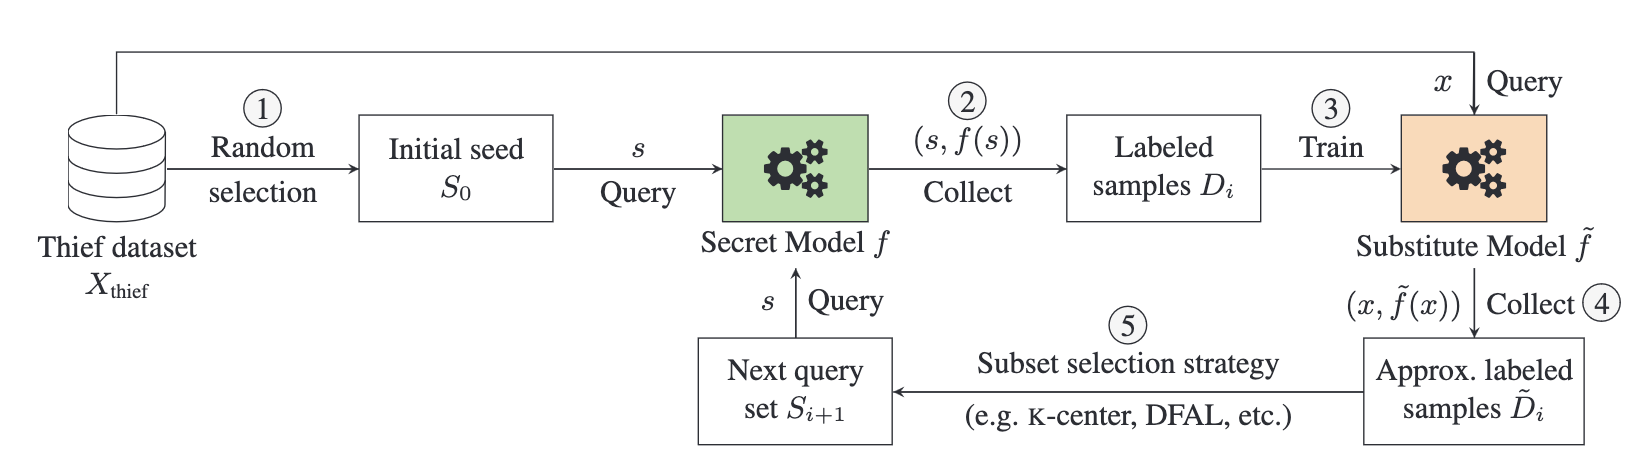
\includegraphics[width=.9\linewidth]{images/ActiveThief_Idea.png}
    \caption[Visualization of ActiveThief]{Illustration of the model stealing workflow proposed by \cite{pal2020activethief}. Inspired by
    \cite{chandrasekaran2020exploring}, Pal et al. use Active Learning to select the next samples to query the target model.}
    \label{fig:ActiveThief}
\end{figure}

%% ---------------------
%% | / Example content |
%% ---------------------
%% LaTeX2e class for student theses
%% sections/methodology.tex
%% 
%% Karlsruhe Institute of Technology
%% Institute for Program Structures and Data Organization
%% Chair for Software Design and Quality (SDQ)
%%
%% Dr.-Ing. Erik Burger
%% burger@kit.edu
%%
%% Version 1.3.6, 2022-09-28

\chapter{Methodology}
\label{ch:Methodolody}

%% -------------------
%% | Example content |
%% -------------------
Since our Continual Learning approach is, to the best of our knowledge, the first approach to combine pool-based Active Learning with Continual
Learning, we explain our approach in detail in this chapter as well as the motivation for it. We then transfer our approach to the domain of Model
Stealing. Because we build upon the framework of ActiveThief, we describe how our method compares to the original one in detail.

\section{Continual Active Learning}
\label{sec:Methodology:ContinualActiveLearning}
A major contribution of this thesis is combining the two learning paradigms of Continual Learning and active learning. To motivate the idea of
combining Continual Learning and Active Learning, we will first outline the classic Continual Learning Setting and the classic Active Learning Setting.
Next, we explain common issues with these two learning paradigms and how we aim to overcome these by combining both paradigms. Finally, we will give
a detailed description of our approach. 

\subsection{The classic Continual Learning Setting}
\label{sec:Methodology:CLSetting}
%Mention that CL Setting consists of multiple tasks, task can and usually are independent
% Outline classic Continual Learning Workflow with a figure
In the typical Continual Learning setting, the model is trained on a sequence of tasks. Each task $T_i = {x_k,y_k | k \in \{1,\ldots,n\}}$ is a set
of instances with their respective label. Together, the tasks form a dataset $D = \bigcup\limits_{i=1}^{N} T_i$. It is important to note that
the distribution of two distinct tasks $P(T_i)$  and $P(T_j) (i \neq j)$ are not necessarily the same. Most often, in fact, the tasks are independent
of each other, which is why neural networks struggle to perform well on multiple tasks at once. This also means that the size of two distinct datasets
can be different, i.e. $|T_i| \neq |T_j|$ and so can the number of classes $|{y_k | \exists x_k: x_k,y_k \in T_i}| \neq |{y_l | \exists x_l: x_l,y_l
\in T_j}|$. When training a model on a sequence of tasks, the model is first fed with the data of the first task $T_1$ and then trained on it. 
After the model was trained on the first task, it can either be trained on the next task or deployed to classify samples stemming from the
distribution of the first task. Next, the model is trained on the second task. After being trained on the second task, the model should now be able to
classify samples from the distribution of the first and second task. This process is repeated until the model has been trained on all
tasks. After being trained on all tasks, the model should be able to classify samples following the distribution of all the tasks it was trained on.
This workflow is illustrated in Figure \ref{fig:CLWorkflow}. \par
The main difference between the Continual Learning setting and classic Machine Learning is that in the classic Machine Learning setting, the model
is never retrained once it is deployed. In the Continual Learning setting, however, the model is retrained whenever a new task arrives.

\begin{figure}[ht]
    \centering
    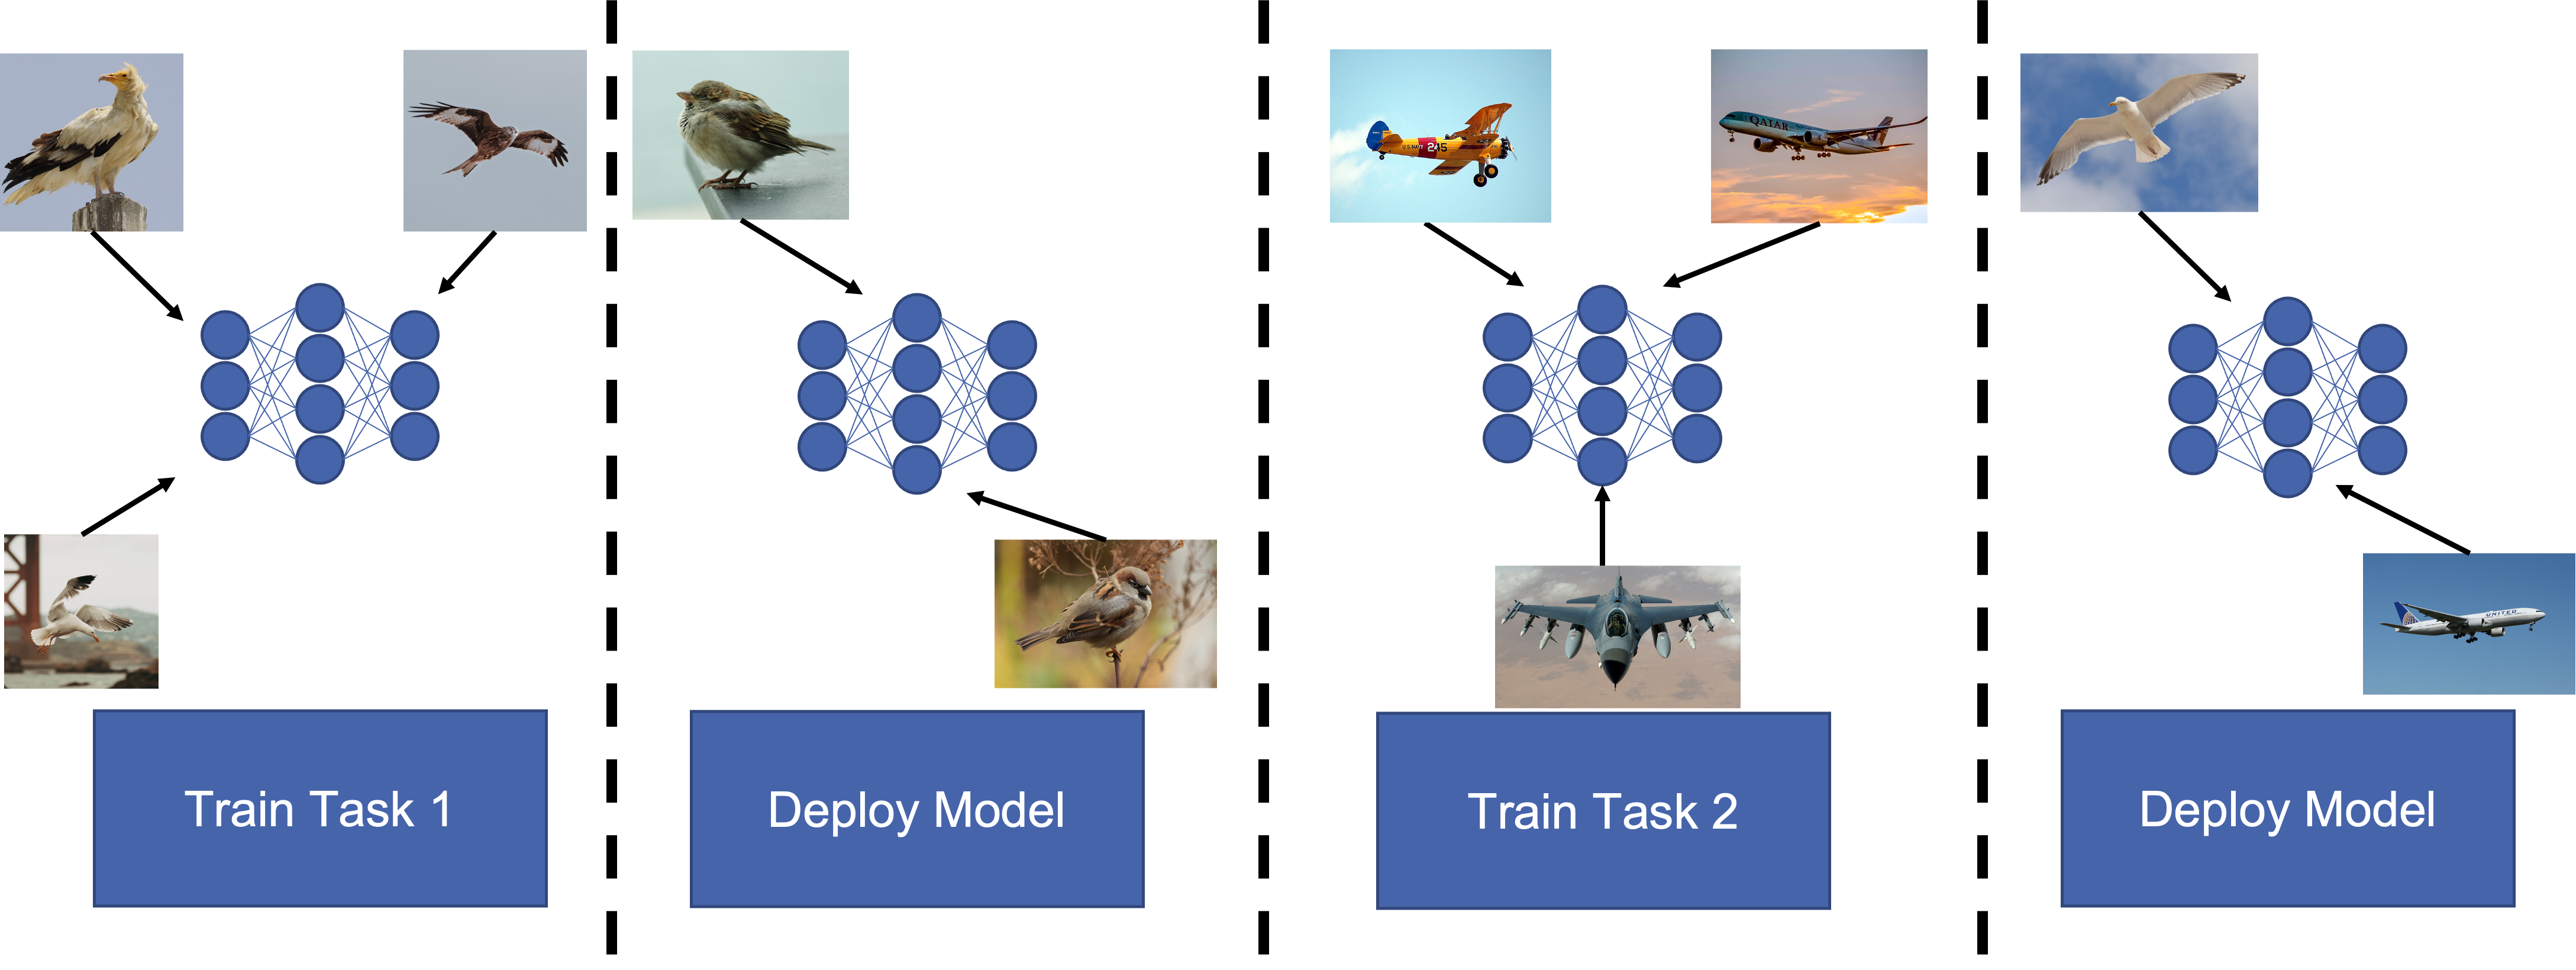
\includegraphics[width=.9\linewidth]{images/CL_workflow.png}
    \caption[Continual Learning Workflow]{Example for the classic Continual Learning Workflow. In this example, the model is first trained on different species of
    birds. It is then deployed to differentiate these species. Next, the model is trained on planes. After being deployed again, the model should now differentiate
    the planes as well as the birds.}
    \label{fig:CLWorkflow}
  \end{figure}

\subsection{The pool-based Active Learning Setting}
\label{sec:Methodology:ALSetting}
%Mention classic pool-based Active Learning setting, what batches are, contrast the continual
% learning setting, saying that the "tasks" are not independent
In the pool-based Active Learning setting, the model is trained sequentially on the current labeled pool. At first, the labeled pool is empty. Next, it is usually
initialized by randomly selecting samples from the unlabeled pool to label. On the contrary, the unlabeled pool contains the full dataset at first and is emptied in the process.
After the labeled pool is initialized, the model is trained on it. Now, until the total budget is exhausted, $b$ samples from the labeled pool are selected which
are determined to be the most informative by the current Active Learning strategy. These samples are then labeled by the oracle and added to the labeled pool. Next, the
model is trained on the current labeled pool, and the process repeats. We provide a more detailed description of pool-based Active Learning in section \ref{sec:PoolBasedActiveLearning}. \par
Active Learning contrasts with Continual Learning in the sense that all data stems from the same task. Another difference between pool-based Active Learning and Continual
Learning is that a model trained by Active Learning is trained on all previously selected batches. Consequently, the model is trained on some data multiple times which
might cause parts of the training to be redundant.
% TODO: Add figure of Active Learning Workflow

\subsection{Combining Continual and Active Learning}
% Mention the issues with the classic CL and AL setting, describe how synergizing the two approaches
% can help overcome these issues and describe the approach in detail
\label{sec:Methodology:CombiningCLandAL}
The problem with classic Active Learning is that it is very resource intensive. When training a model using pool-based Active Learning on a dataset of size $n$,
with batch size $b$, the model will be trained $\frac{n}{b}$ times on the current labeled pool, equating to $\frac{n(n+b)}{2b}$ data points overall (we provide a
short derivation of this number in \ref{sec:appendix:FirstSection}). The problem with the number of data points used for training is that it is dependent on the
batch size $b$. The smaller the batch size, the larger the overall number of data points that the model is trained on. In the extreme case of $b=1$, the model
is trained on $\frac{n(n+1)}{2}$ data points. While \cite{beck2021effective} note that the batch size has a negligible effect on the model performance,
if any, a typical batch size is less than 10 \% of the full training set. Even in this more realistic case, the model is trained on $5.5n$ data points. When
comparing this to the classic Continual Learning setting, where the model is trained once using $n$ data points, it is clear that Active Learning comes
with considerable overhead. The overhead of Active Learning is even more pronounced when considering the running time of the Active Learning Algorithms.
For more details, we refer to Chapter \ref{ch:Evaluation} and \ref{ch:Discussion}. \par
On the other hand, a major problem with classic Continual Learning is that task order significantly impacts the model performance \cite{bell2022effect}.
The problem of task ordering has been studied before, and it has been shown that training samples in decreasing order of difficulty results in faster learning and 
improved generalization error \cite{hacohen2019power}. This motivates us to use Active Learning to perform task ordering. We should note here that we
assume the free choice of the next task. This assumption is not always realistic, especially when tasks arrive sequentially, but studying the effect of task-ordering
benefits the study of these scenarios, too. Furthermore, insights into task-ordering help towards a more rigorous evaluation of Continual Learning in 
research because they allow us to assess the influence of task-ordering on experiment results when using classic benchmark datasets. \par
Our approach aims to overcome the issue of the overhead of Active Learning and the issue of task ordering by combining both learning paradigms. We modify the Active
Learning process by training only on the currently selected batch instead of the entire labeled pool. This way, the model is trained on $\sum_{i=1}^{\frac{n}{b}} b = n$ 
data points, which fully eliminates the overhead of Active Learning from a data-centric perspective. Nevertheless, the query time of the Active Learning Algorithm remains
an overhead. From a Continual Learning perspective, we join all tasks to a single dataset and use this dataset as the unlabeled pool for Active Learning. In each iteration
of the Active Learning process, we select a batch $B$ of data points from the unlabeled pool using the given Active Learning Strategy. Next, the oracle labels this batch
if the initial dataset was unlabeled. If the initial dataset is labeled, we omit to query the oracle because the label is already known and simply add the labels
to the respective data points. We then treat the current batch $B$ as a new task and train our model using only the data points of $B$ with the Continual Learning strategy of
choice. This process is repeated until the unlabeled pool is empty. The full algorithm is described in Algorithm \ref{alg:PoolBasedContinualActiveLearning} where we high-
light the difference between classic pool-based Active Learning and our new Continual Active Learning approach in red. \par
%TODO: Mention here that we aim to increase the efficiency of the training process, i.e. we save time because we train on less
% data points

\begin{algorithm}
    \caption{Pool-based Continual Active Learning} \label{alg:PoolBasedContinualActiveLearning}
    \begin{algorithmic}[1]
        \Require Unlabeled data $U$,Labeled data $L = \emptyset$:, Oracle $O$, Model $M$, budget $B$
        \State Select $k$ data points from $U$ at random, obtain labels by querying $O$ and set $L=\{x_1,\ldots,x_1\}$
        and $U = U \setminus \{x_1,\ldots,x_1\}$ \Comment{Initialization}
        \State Train $M$ on initial labeled set $L$
        \While{label budget $B$ not exhausted}
            \State Select $l$ data points from $U$ predicted to be the most informative by the Active Learning strategy
            \State Obtain labels $y_i,\ldots,y_l$ by querying $O$ for $x_i,\ldots,x_l$
            \State {\color{red} Train $M$ on current labeled batch $\{(x_iy_i),\ldots,(x_l,y_l)\}$}
            \State Set $L= L \cup \{x_i,\ldots,x_l\}$ and $U = U \setminus \{x_i,\ldots,x_l\}$
            \State Train $M$ on labeled set $L$
        \EndWhile
    \end{algorithmic}
\end{algorithm}

\section{Continual Active Learning for Model Stealing}
\label{sec:Methodolody:CALMS}
% Transition to model stealing and elaborate why the continual active learning approach is interesting
% in the model stealing domain. Explain how the continual active learning approach has to be modified
% to apply it to model stealing. Best use a figure similar to the figure explaining the CAL approach
% and highlight the parts that are different
In this section, we describe how we apply the Continual Active Learning approach to the problem of model stealing. Using the Continual Active Learning approach
in the model stealing domain allows us to determine if the Continual Active Learning achieves similar performance in the model stealing domain compared to
the standard setup where the oracle returns truthful labels. To motivate transferring our approach to the Active Learning domain, it is crucial to highlight the
differences between the setup mentioned in \ref{sec:Methodology:CombiningCLandAL} and Continual Active Learning for Model Stealing. \par
The first difference is that the labels returned by the oracle in the model stealing domain have a limited semantic meaning. This is because the oracle is another
Machine Learning model in the model stealing domain. So even if the data point whose label is queried stems from the same distribution as the target model dataset,
the label returned by the oracle is not necessarily correct since Machine Learning Models are not capable of generalizing perfectly. Since the target model dataset
is unknown to the attacker, he or she cannot knowingly construct a thief dataset that overlaps with the target model dataset. Therefore, the data points that the
attacker queries the target model with will most likely be from a different distribution than the target model dataset and the labels returned by the target model
will be incorrect. The example in Figure \ref{fig:CalmsWorkflow} highlights the meaning of the associated label. In the given example, the target model is trained
to classify planes which is why it associates the label \enquote{Fighter Jet} with a sparrow. \par
The second difference between the standard Continual Active Learning approach and Continual Active Learning for Model Stealing lies again in the labels returned by
the oracle. In the classic Continual Active Learning approach, the labels of the oracle are not only truthful, but the label is just a single value, i.e. the respective
class. In the model stealing domain, the label returned by the oracle is either a single value or the per-class probabilities of the output layer of the target model.
The latter is the more interesting case for Continual Active Learning because it reveals much more information about the function learned by the target model. \par
After explaining the motivation for applying the Continual Active Learning approach to the model stealing domain, we now describe how Continual Active Learning can be
applied for model stealing. The first step is to use the thief dataset as the initial unlabeled pool for Active Learning. The Active Learning
strategy uses the thief dataset in each iteration as it would have been done in classic Continual Active Learning. After selecting the most informative samples to label,
the target model is queried for the labels of the selected samples. Next, the label returned, which is either a single value or the per-class probabilities of the output
layer of the target model, is used as the label of the respective data point throughout the entire training process. This means specifically that the gradient updates during 
training are based on the loss computed with a softmax label, allowing for a more fine-grained optimization of the weights to approximate the target model function. This
process is repeated until the unlabeled pool is empty. A visual example of the Continual Active Learning for Model Stealing workflow is shown in Figure
\ref{fig:CalmsWorkflow}. \par
\begin{figure}[ht]
    \centering
    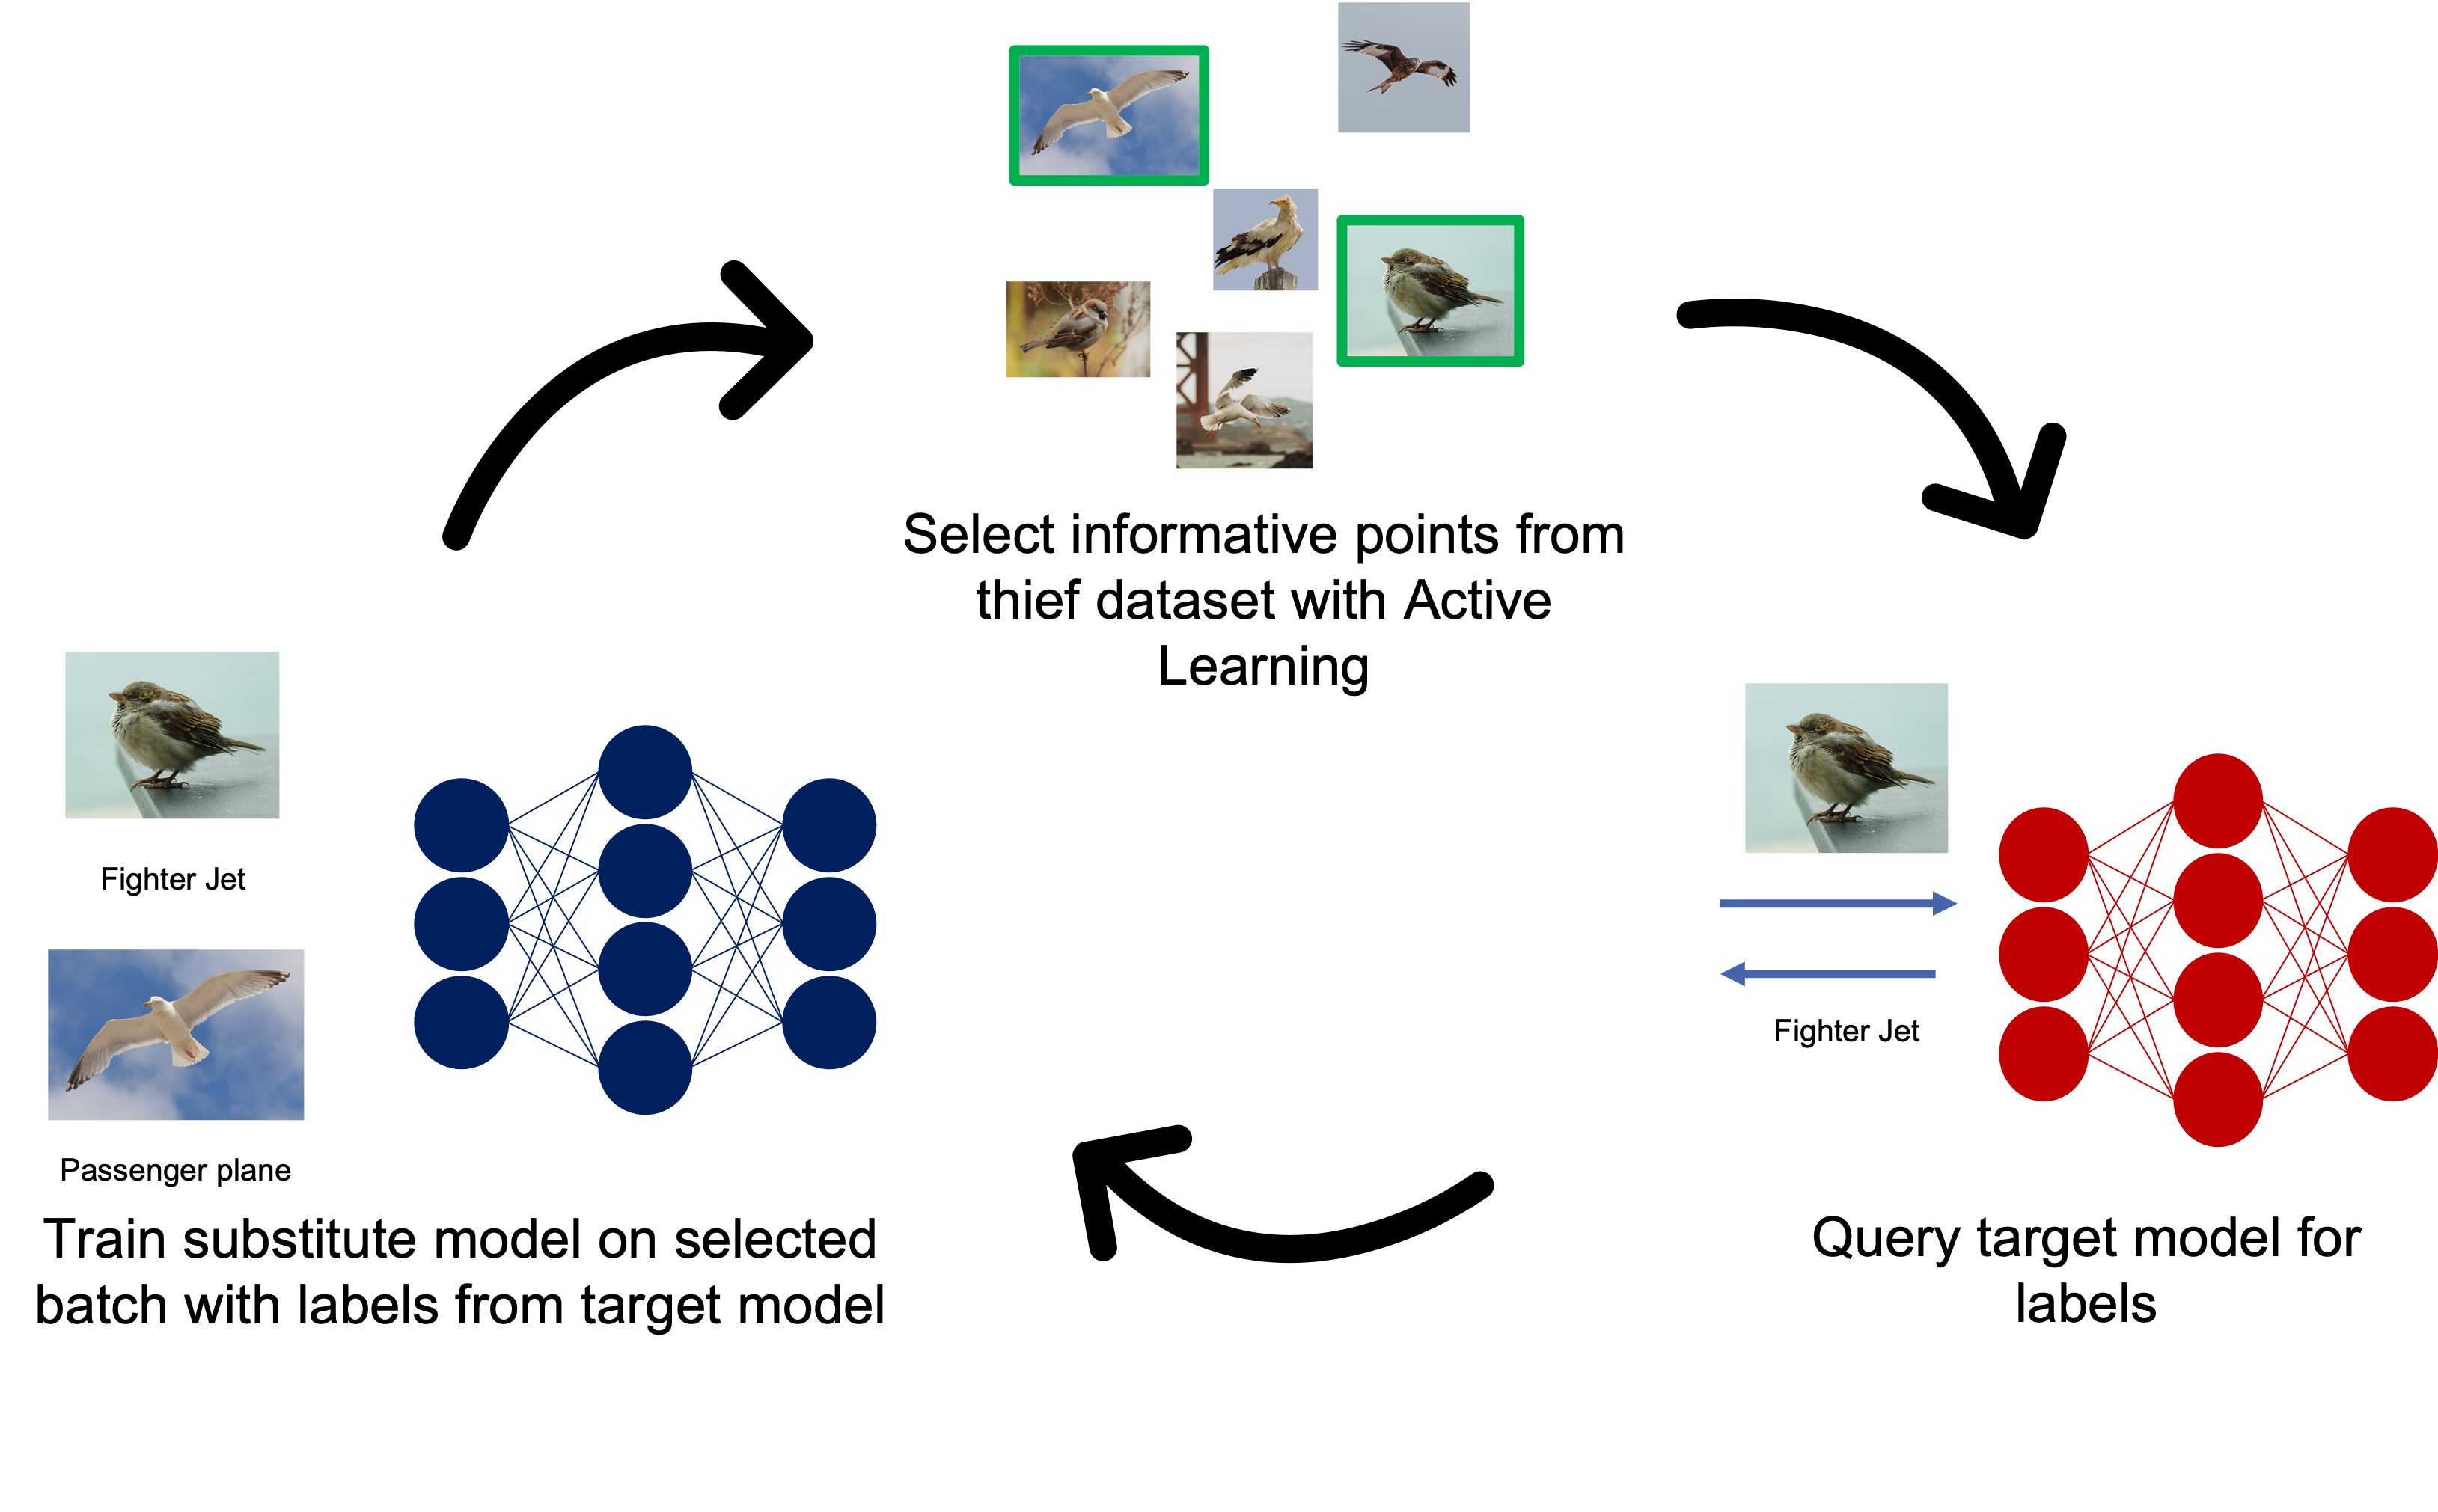
\includegraphics[width=.9\linewidth]{images/Calms_workflow.png}
    \caption[Continual Active Learning for Model Stealing Workflow]{Example of the Continual Active Learning for Model Stealing Workflow. In this example, the thief
    dataset consists of birds while the target model was trained to classify planes. In each iteration, a batch of informative samples is selected by the Active Learning
    strategy first. Next, the target model is queried for the labels of the selected samples. Since our thief dataset is composed of NNPD data, the associated labels have
    an incorrect semantic meaning. The thief model is then trained only on the selected samples from the current batch. This process is repeated iteratively.}
    \label{fig:CalmsWorkflow}
\end{figure}

\section{Replay strategy}
\label{sec:Methodology:ReplayStrategy}
In this section, we propose a Continual Learning Strategy called Replay. Applying replay to overcome catastrophic forgetting is not an entirely new idea. In fact, it
has been proposed since the 1990s \cite{robins1995catastrophic}. The approach we propose modifies the classic replay by compressing the replay buffer. To understand the modification
we must first understand the classic replay strategy. \par
Replay is a Continual Learning strategy that stores a subset (or all) data points from each task in a so-called replay buffer. When training on a new task $T_N$, the model is trained 
on all data from the current task plus a sample from the replay buffer. After training on task $T_N$, the replay buffer is updated with the data points from the current task. \par
A significant drawback of the classic Replay strategy is that the replay buffer can grow to extreme sizes over time. This is especially true when the replay buffer stores all data points from
each task. It is more desirable to have a Continual Learning strategy with a fixed memory footprint because this reflects the realistic application of Continual Learning where memory 
is limited. \par
The proposed modification of the Replay strategy is to compress the replay buffer after each task. Assume we have a replay buffer of size $n$. After training on task $T_N$, the replay buffer
is combined with the data points from the current task to form a new set of data points $P$. We then select $n$ data points from $P$ to form the new replay buffer. The selection of the $n$ data
is done by performing one iteration of the Active Learning strategy CoreSet \cite{sener2018active} with $P$ as the unlabeled pool and $n$ as the batch size. The $n$ data points selected by Core-
Set then represent the new replay buffer. When training on task $T_{N+1}$, the model is trained on all data from the current task plus the full replay buffer.

%% ---------------------
%% | / Example content |
%% ---------------------
%% LaTeX2e class for student theses
%% sections/methodology.tex
%% 
%% Karlsruhe Institute of Technology
%% Institute for Program Structures and Data Organization
%% Chair for Software Design and Quality (SDQ)
%%
%% Dr.-Ing. Erik Burger
%% burger@kit.edu
%%
%% Version 1.3.6, 2022-09-28

\chapter{Experiment Setup}
\label{ch:ExperimentSetup}
% Describe hardware and software specification, datasets used, models used.
% Specifically mention which datasets are target datasets for model stealing
% and which are thief datasets
The findings of this thesis rely heavily on thorough experimentation. To reproduce our experiments, we specify the
conditions under which we conducted the experiments. This includes training hyperparameters, datasets, neural network architectures,
and information about the code and libraries used. In general, we divide our experiments into two categories: Experiments that explore
the classic continual active learning setting as in section \ref{sec:Methodology:CombiningCLandAL} and experiments that explore continual 
active learning for model stealing as in section \ref{sec:Methodolody:CALMS}. We perform this differentiation because many 
training hyperparameters, datasets, and neural network architectures depend on whether we evaluate classic continual active learning or continual 
active learning for model stealing. First, we mention the general setup, including hardware, software, datasets, and the training
hyperparameters shared between the two categories of experiments. Next, we list the specific configuration for
continual active learning and continual active learning for model stealing. Finally, we mention the evaluation metrics used in our experiments.

\section{General Experiment Setup}
\label{sec:ExperimentSetup:FirstSection}
In this section, we describe the general experiment setup. The parameters described in this section are shared across all experiments, unless
explicitly stated otherwise.

\subsection{Hardware}
All experiments are conducted on the \gls{hpc} cluster bwUniCluster 2.0 \cite{bwUnicluster}. bwUniCluster 2.0 is an \gls{hpc} cluster
funded by the Ministry of Science, Research and the Arts Baden-Württemberg and the Universities of the State of Baden-Württemberg. It currently consists
of more than 840 compute nodes with each node falling one of the following categories: \enquote{Thin}, \enquote{HPC}, \enquote{IceLake}, \enquote{Fat},
\enquote{GPUx4}, \enquote{GPUx8}, \enquote{GPUx4 A100}, \enquote{GPUx4 H100} and \enquote{Login}. In our experiments, we use the nodes GPUx4, GPUx8 and
GPUx4 A100. We list their hardware specifications in appendix \ref{sec:Appendix:Software}. Furthermore, we conduct experiments where we
measure runtime on the GPUx8 nodes.

\subsection{Software and Libraries}
\label{sec:ExperimentSetup:Software}
All the code used in this thesis is written in version 3.9.4 of the programming language Python \cite{Rossum1995Python}. Furthermore, we use the deep
learning library PyTorch \cite{paszke2019pytorch} (version 1.13.1) to implement both active and continual learning algorithms. All further libraries
and their respective versions can be found in appendix \ref{sec:Appendix:Software}.

\subsection{Continual Learning Strategies}
\label{sec:ExperimentSetup:CLStrategies}
In our experiments, we use the continual learning strategies \gls{ewc}, \gls{mas}, \gls{imm}, \gls{alasso}, \gls{a-gem} and our custom Replay strategy
proposed in section \ref{sec:Methodology:ReplayStrategy}. For details on these continual learning strategies, we refer to section 
\ref{sec:Related_work:Continual_Learning}. As a baseline, we used the naive strategy of performing classic gradient descent without 
regularization. In the following, we will refer to this strategy as Naive. \par
Following the paper introducing \gls{mas} \cite{aljundi2018memory}, we set the regularization parameter $\lambda$ to 1.0 for \gls{mas}. The choice of
this parameter is crucial because it enables a sound evaluation. If we trivially chose to set $\lambda$ to 0, there would be no difference between
\gls{mas} and the naive strategy. On the other hand, fine-tuning is neither possible (we use more than 25 combinations of continual learning strategies and
active learning strategies on three datasets) nor fair (to evaluate the quality and effect of all continual learning strategies, they should be tested under
the same conditions). We, therefore, set $\lambda$ in \gls{ewc} and \gls{imm} to 1.0 accordingly.
The regularization parameter $c$ in \gls{alasso}, which is equivalent to $\lambda$ in \gls{ewc}, \gls{mas}, and \gls{imm} is set to 0.5 for all experiments.
We tried setting $c$ to 1.0, however, we noticed that this led to divergence during gradient descent despite employing heavy gradient clipping. Since employing
stronger gradient clipping was not a viable solution, because it impedes model convergence, we decided to relax the regularization parameter $c$ to 0.5. \par
As mentioned, we employ gradient clipping to ensure convergence of gradient descent. Not only is gradient clipping a remedy against the exploding
gradient problem, but Zhang et al. have demonstrated, that it can accelerate the training process \cite{zhang2019gradient}. In our implementation, we clip gradients by their
$l_2$ norm. Across all continual learning procedures, including Naive, we clip the gradients to a maximum $l_2$ norm of 20.0 to accelerate the training process.
When conducting experiments with \gls{mas} and \gls{alasso} we encountered exploding gradient problems, which we further investigated for \gls{mas} and \gls{alasso}
separately. While we aimed to eliminate the exploding gradient problem, which is mitigated more by clipping smaller gradients, we did not want to restrict the
model too much to hinder model convergence. After carefully exploring different values to clip at, we found setting the threshold for the $l_2$-Norm to 2.0
to be effective, mitigating the exploding gradient problem while simultaneously enabling model convergence. \par
Apart from the parameter weighting of the regularization term, the continual learning strategies do not share any hyperparameters. \gls{ewc} does not have
any further hyperparameters, and neither does \gls{mas}. On the other hand, for \gls{imm}, we have the choice between mean-\gls{imm} and mode-\gls{imm}. Furthermore,
we can choose to apply weight-transfer, $l_2$-transfer, and dropout-transfer, and we can choose values for the parameter $\alpha$. In our setup, we use mean-\gls{imm},
weight-transfer and $l_2$-transfer and set the $\alpha$ parameter to [0.45,0.55] (i.e. $\alpha_1 = 0.45, \alpha_2 = 0.55$), as suggested by the authors. Both \gls{ewc} and
\gls{imm} use Fisher information to determine parameter importance. To compute the \gls{fim}, we use five percent of the training set of the current task.
Regarding \gls{alasso}, we set the parameter $a$, which controls the overestimation on the unobserved side, to 3.0. Following the authors' recommendation,
we perform parameter decoupling for the $\Omega$ updates. Therefore, we set $a'$ to 1.5 and $c'$ to 0.25. For \gls{a-gem}, we set $S$, the number of samples
drawn from the episodic memory to compute the reference gradients, to 2,000. The second hyperparameter, $P$, which controls the number of patterns from a task
saved to the memory, is also set to 2,000. \par
We provide a detailed summary of the hyperparameters used in appendix \ref{sec:Appendix:CLStrategies}.


\subsection{Active Learning Strategies}
\label{sec:ExperimentSetup:ALStrategies}
In our experiments, we use the active learning strategies \gls{badge}, \gls{lc}, CoreSet, \gls{bald}, and \gls{vaal}. For details on these active learning
strategies, we refer to section \ref{sec:Related_work:Active_Learning}. For \gls{badge}, we use the Euclidean distance in the $k$-means++
algorithm. For CoreSet, we use the Euclidean distance between the activations of the penultimate layer of the neural network as a distance metric for $k$-Center
algorithm. For \gls{bald}, we use the Monte Carlo dropout with $T=25$ samples. We omit Monte Carlo dropout in cases where the model does not contain dropout layers,
as the prediction of such a model is deterministic. \gls{lc} does not contain hyperparameters. For \gls{vaal}, we train \gls{vae} and discriminator for 20 epochs
per iteration. We use the neural network architecture and training hyperparameters from the GitHub repository published by the authors along with the paper 
\cite{vaalRepo}. \par
Across all active learning strategies, we use the same initial budget, i.e., the number of points we sample from the training set before the first iteration
of the active learning algorithm. In our experiments, we set the initial budget to be the same as the batch size.

\subsection{Datasets}
\label{sec:ExperimentSetup:Datasets}
In our experiments, we use the datasets MNIST \cite{mnist_web}, CIFAR-10 \cite{cifar},
CIFAR-100 \cite{cifar}, Tiny ImageNet \cite{le2015tiny}, and a subset of the ILSVRC2012-14 dataset \cite{imagenet}. The subset of the ILSVRC2012-14 dataset we
use is the first of ten training batches downloaded from \cite{imageNetDataset}. From now on, we will refer to this subset
of the ILSVRC2012-14 dataset as Small ImageNet. For all datasets, we use the standard train test split, as proposed by PyTorch. We rescale all images to 32x32
pixels, because for the success of a model stealing attack, the image shape of the thief dataset has to match the image shape accepted by the target model. We will cover
this in more detail in section \ref{sec:Methodology:CALMSsetup}. Moreover, we normalize the train and test split of all datasets by using the mean and standard deviation
of the training set. On all datasets, apart from MNIST, we apply data augmentation. We use random horizontal flips with a probability of 0.5
followed by random cropping. We provide a detailed list of the datasets used in appendix \ref{sec:Appendix:Datasets}. \par

\subsection{Neural Network Architectures}
\label{sec:ExperimentSetup:NNArchitectures}
We use the neural network architectures ResNet18 \cite{he2016deep} and \gls{cnn} architectures from the ActiveThief paper \cite{pal2020activethief} in our experiments.
In the following, we will refer to this \gls{cnn} architecture as \enquote{ActiveThiefConv}. Since there are multiple variations of the architecture, more specifically
ones with two, three, or four convolutional blocks, we will refer to those as ActiveThiefConv2, ActiveThiefConv3, and ActiveThiefConv4, respectively. We present the
layout of the three ActiveThiefConv architectures in appendix \ref{sec:Appendix:Architectures}.


\subsection{Training Hyperparameters}
\label{sec:ExperimentSetup:Hyperparameters}
We use PyTorch's \gls{sgd} optimizer with a learning rate of 0.1 across all experiments. Furthermore, we schedule the learning rate by a factor of 0.1. The number of
epochs after which we schedule the learning rate differs between experiments. Furthermore, we re-instantiate the \gls{sgd} optimizer after each active learning
iteration. We will go into detail on this in the description of the respective experiments. Apart from scheduling the learning rate, we use momentum \cite{cutkosky2020momentum}
of 0.9 and $l_2$ regularization of 0.0005. For all experiments, we use a batch size of 128 and shuffle the entire training set before each epoch.


\section{Special Setup for Continual Active Learning}
\label{sec:Methodology:CALsetup}
We experiment with continual active learning using ResNet18 as our neural network architecture and CIFAR-10 as our dataset. We perform experiments with a batch size of 1,000,
2,000 and 4,000, respectively. Regardless of the batch size, we conduct active learning until the unlabeled pool is exhausted. This means that we perform active learning for
49, 24, and 12 iterations, respectively. For batch sizes 1,000 and 2,000, each query consists of 1,000 and 2,000 points, respectively, while the last query for batch size 4,000 consists of 2,000 points.
For batch sizes 2,000 and 4,000, we train for 150 epochs per iteration, decaying the learning rate by ten after 80 and 120 epochs, respectively. For batch size 1,000, we
train for 80 epochs and decay the learning rate by ten after 60 epochs. To compare the performance of continual active learning with active learning, we computed the results
for active learning with identical batch sizes. In this experiment setup, we use warm start and train for 200 epochs in each iteration. Here, we
decay the learning rate by ten after 100 and 150 epochs, respectively.

\section{Special Setup for Continual Active Learning for Model Stealing}
\label{sec:Methodology:CALMSsetup}
When transferring continual active learning to the model stealing domain, we change our setup compared to continual active learning previously. Instead of using ResNet18 as our
model architecture, we use the \gls{cnn} architecture from the ActiveThief paper \cite{pal2020activethief}, mainly because we want to compare our continual active learning approach to
the framework proposed by the authors of ActiveThief. For most of our experiments, we use ActiveThiefConv3 apart from experiments investigating the effect of the model 
architecture on model stealing attacks. We train the target models on the datasets CIFAR-10, CIFAR-100, and MNIST. We train the target models on CIFAR-10 and CIFAR-100 for
150 epochs using a momentum of 0.9 and $l_2$ regularization of 0.0005 without learning rate decay. When training the target models on MNIST, we change the number of epochs to 50.
We omit to retrain the target model for all model stealing attacks. Instead, we train one target model per dataset, save them to the disk and load them for all model stealing
attacks. This way, we reduce the uncertainty in our experiments introduced by different weight initializations of the target model. We use Small ImageNet as our thief dataset for all model stealing attacks. \par
Similar to the classic continual learning setting, we compute a baseline with active learning for model stealing. For this baseline, we use active learning with a batch size of 1,000
and a total budget of 20,000 points. The models are trained using cold start for 200 epochs per iteration. We decay the learning rate by ten after 100 and 150 epochs. \par
For continual active learning for model stealing, we use a batch size of 2,000 and a total budget of 20,000. We decided to increase the batch size for continual active learning compared
to pure active learning because we noticed a clear correlation between batch size and model performance when training using continual active learning. We train the substitute model for
150 epochs per iteration and decay the learning rate by ten after 80 and 120 epochs with a momentum of and $l_2$ regularization of 0.0005.

\section{Evaluation Metrics}
\label{sec:Methodology:Metrics}
We describe and motivate the metrics for the evaluation of continual active learning in this section. Since we use continual active learning in two distinct
domains, we will discuss the metrics for each domain separately. We will start with the metrics for the classic continual learning setting and then move on to the
metrics for the model stealing domain.

\subsection{Metrics for Continual Active Learning}
\label{sec:Methodology:Metrics:CAL}
When choosing a metric to evaluate continual active learning, we should remember why we proposed the approach. The aim of continual active learning is to mitigate the
overhead of active learning compared to the classic training loop. Therefore, it is desirable to incorporate a metric that measures this goal. In our case, this is
the overall execution time. However, execution time is not the only metric we want to use to evaluate the approach. Since the second goal of the continual learning
approach is to improve model performance, we will also evaluate the experiments based on this. What makes a machine learning model performant has been discussed vividly
in the literature \cite{flach2019performance}. In our case, we will use the validation accuracy as a metric to evaluate model performance. When we evaluate the experiments,
we need to consider \textit{both} runtime and validation accuracy. A model with low runtime and validation accuracy is not desirable,
but neither is a model with high runtime and validation accuracy. Since we are trying to improve active learning by introducing continual learning into the pool-based 
active learning process, we aim to outperform the classic pool-based active learning approach. More precisely, we want to reduce the runtime and increase the validation
accuracy. We will evaluate the success of our continual active learning approach against the classic pool-based active learning approach based on the runtime improvement
and the accuracy improvement. 


\subsection{Metrics for Continual Active Learning for Model Stealing}
\label{sec:Methodlogy:Metrics:CALMS}
As presented in section \ref{sec:ModelStealing:Attacks}, model stealing attacks can be performed for multiple reasons. As we build our framework on ActiveThief, we adopt
the metrics used in the original paper. The ActiveThief framework aims purely at stealing the model functionality, i.e., approximating the model's relationship
between input and output best, and so does ours. Therefore, we will use the same evaluation metric, the agreement between the substitute and target model,
computed on the validation split of the target model dataset. For an explanation of the model agreement metric, we refer the reader to section \ref{sec:ModelStealing:Terminology}.
The baseline which we compare our results against is the ActiveThief framework. We will therefore measure the success of using continual active learning for model stealing by comparing
the model agreement of our approach to the model agreement of the ActiveThief framework.

%% LaTeX2e class for student theses
%% sections/evaluation.tex
%% 
%% Karlsruhe Institute of Technology
%% Institute for Program Structures and Data Organization
%% Chair for Software Design and Quality (SDQ)
%%
%% Dr.-Ing. Erik Burger
%% burger@kit.edu
%%
%% Version 1.3.6, 2022-09-28

\chapter{Evaluation}
\label{ch:Evaluation}

In the following chapter we will evaluate the experiments we conducted. We start off by explaining our evaluation metrics, both for Continual Active Learning
and when applying Continual Active Learning to Model Stealing. Afterwards we will present the results of our experiments and discuss the findings.

\section{Evaluation Metrics}
\label{sec:Evaluation:Metrics}
% Describe that we used agreement for model stealing (and on which dataset) and 
% validation accuracy for the model stealing experiments. and hyperparameters

\subsection{Metrics for Continual Active Learning}
\label{sec:Evaluation:Metrics:CAL}
When choosing a metric to evaluate Continual Active Learning, we need to remember the motivation of the approach. We proposed the Continual Active Learning approach
mainly to reduce the mainly to mitigate the overhead of pure Active Learning compared to the classic training loop. Therefore, it is desirable to incorporate a metric
which measures this goal. In our case, this is the overall execution time. However, execution time is not the only metric we want to use to evaluate the approach. Since 
the second goal of the Continual Learning approach is to improve model performance, we will also evaluate the experiments based on this. What a makes a machine learning 
model performant has been discussed vividly in the literature. In our case, we will use the validation accuracy as a metric to evaluate the performance of the model. It is
important to consider \textit{both} runtime and validation accuracy when evaluating the experiments. A model with low runtime and low validation accuracy is not desirable,
but neither is a model with high runtime and high validation accuracy. Since we are trying to improve Active Learning by introducing Continual Learning into the pool-based 
Active Learning process, we aim to outperform the classic pool-based Active Learning approach. More precisely, we want to reduce the runtime and increase the validation
accuracy. The success of our Continual Active Learning approach will be evaluated against the classic pool-based Active Learning approach based on the runtime improvement
and the accuracy improvement. 


\subsection{Metrics for Continual Active Learning for Model Stealing}
\label{sec:Evaluation:Metrics:CALMS}
As presented in section \ref{sec:ModelStealing:Attacks}, Model Stealing Attacks can be performed for a variety of reasons. As we build our framework on ActiveThief, we also
adopt the metrics used in the original paper. The ActiveThief framework aims purely at stealing the functionality of the model, i.e. approximation the model's relationship
between input and output best, and so does ours. Therefore, we will use the same evaluation metric, which in our case is the agreement between substitute and target model,
computed on the validation split of the target model dataset. For an explanation of the Model Agreement metric, we refer the reader to section \ref{sec:ModelStealing:Terminology}.
The baseline which we compare our results against is the ActiveThief framework. We will therefore measure the success of using Continual Active Learning for Model Stealing by comparing
the model agreement of our approach to the model agreement of the ActiveThief framework.

\section{Results}
\label{sec:Evaluation:Results}
In this section we will present the results of our experiments. As mentioned before, our experiments are split into two parts. The first part is the evaluation of our novel
Continual Active Learning Approach and the second part is evaluating the performance our the Continual Active Learning approach when applied to Model Stealing. In each of these
respective subsections we will first describe the experiments schedule for each part and then present the results of the experiments.

\subsection{Results for Continual Active Learning}
\label{sec:Evaluation:Results:CAL}
In this subsection we will first present the results of running all combinations of the Active Learning strategies \gls{bald},\gls{badge},CoreSet,\gls{lc} and Random with the Continual Learning strategies
Naive, \gls{ewc}, \gls{mas}, \gls{alasso} and \gls{imm}. Afterwards, we will analyze the behavior of a hybrid approach between Active Learning and Continual Active Learning, where we first run a few cycles with
pure Active Learning before switching to Continual Active Learning. We further analyze the performance of different strategies to initialize the labeled pool. Next, we experiment with \gls{vaal}
and \gls{a-gem}.

\subsubsection{AL and Cl combinations}
\label{sec:Evaluation:Results:CAL:ALCL}
To evaluate the combination of the Active Learning strategies \gls{bald},\gls{badge},Coreset,\gls{lc} and Random with the Continual Learning strategies Naive, \gls{ewc}, \gls{mas}, \gls{alasso} and \gls{imm}, we run each combination
using a batch size of 1000,2000 and 4000. We use the CIFAR-10 dataset and the Neural Network Architecture Resnet18 for these experiments. We present the validation accuracy with increasing
size of the labeled pool as well as the overall runtime of each experiment. \par
In figure \ref{fig:Evaluation:Results:CAL:Random1000} we present the results of running the Active Learning strategy Random with the Continual Learning strategies Naive, \gls{ewc}, \gls{mas}, \gls{alasso} and \gls{imm}
as well as the baseline of running pure Active Learning. We use a batch size of 1000 for these experiments. In terms of runtime, all strategies are significantly faster than the classic Active
Learning approach. \gls{mas}, \gls{imm}, \gls{ewc} and Naive all are approximately 50 times as fast as the classic Active Learning approach. \gls{alasso} is slightly slower than the other Continual Learning strategies,
but still about 25 times faster than the baseline. However, there is a notable gap in validation accuracy between Active Learning and all Continual Active Learning strategies. \gls{imm} is the only
Continual Learning strategy to outperform the Naive approach. \gls{ewc} performs slightly worse Naive while \gls{mas} and \gls{alasso} perform significantly worse. While the validation accuracy of \gls{mas} increases only
slightly with an increasing size of the labeled pool, \gls{alasso} has an erratic validation curve which does not seem to stabilize until the end of the experiment. \par
\begin{figure}[h]
    \centering
    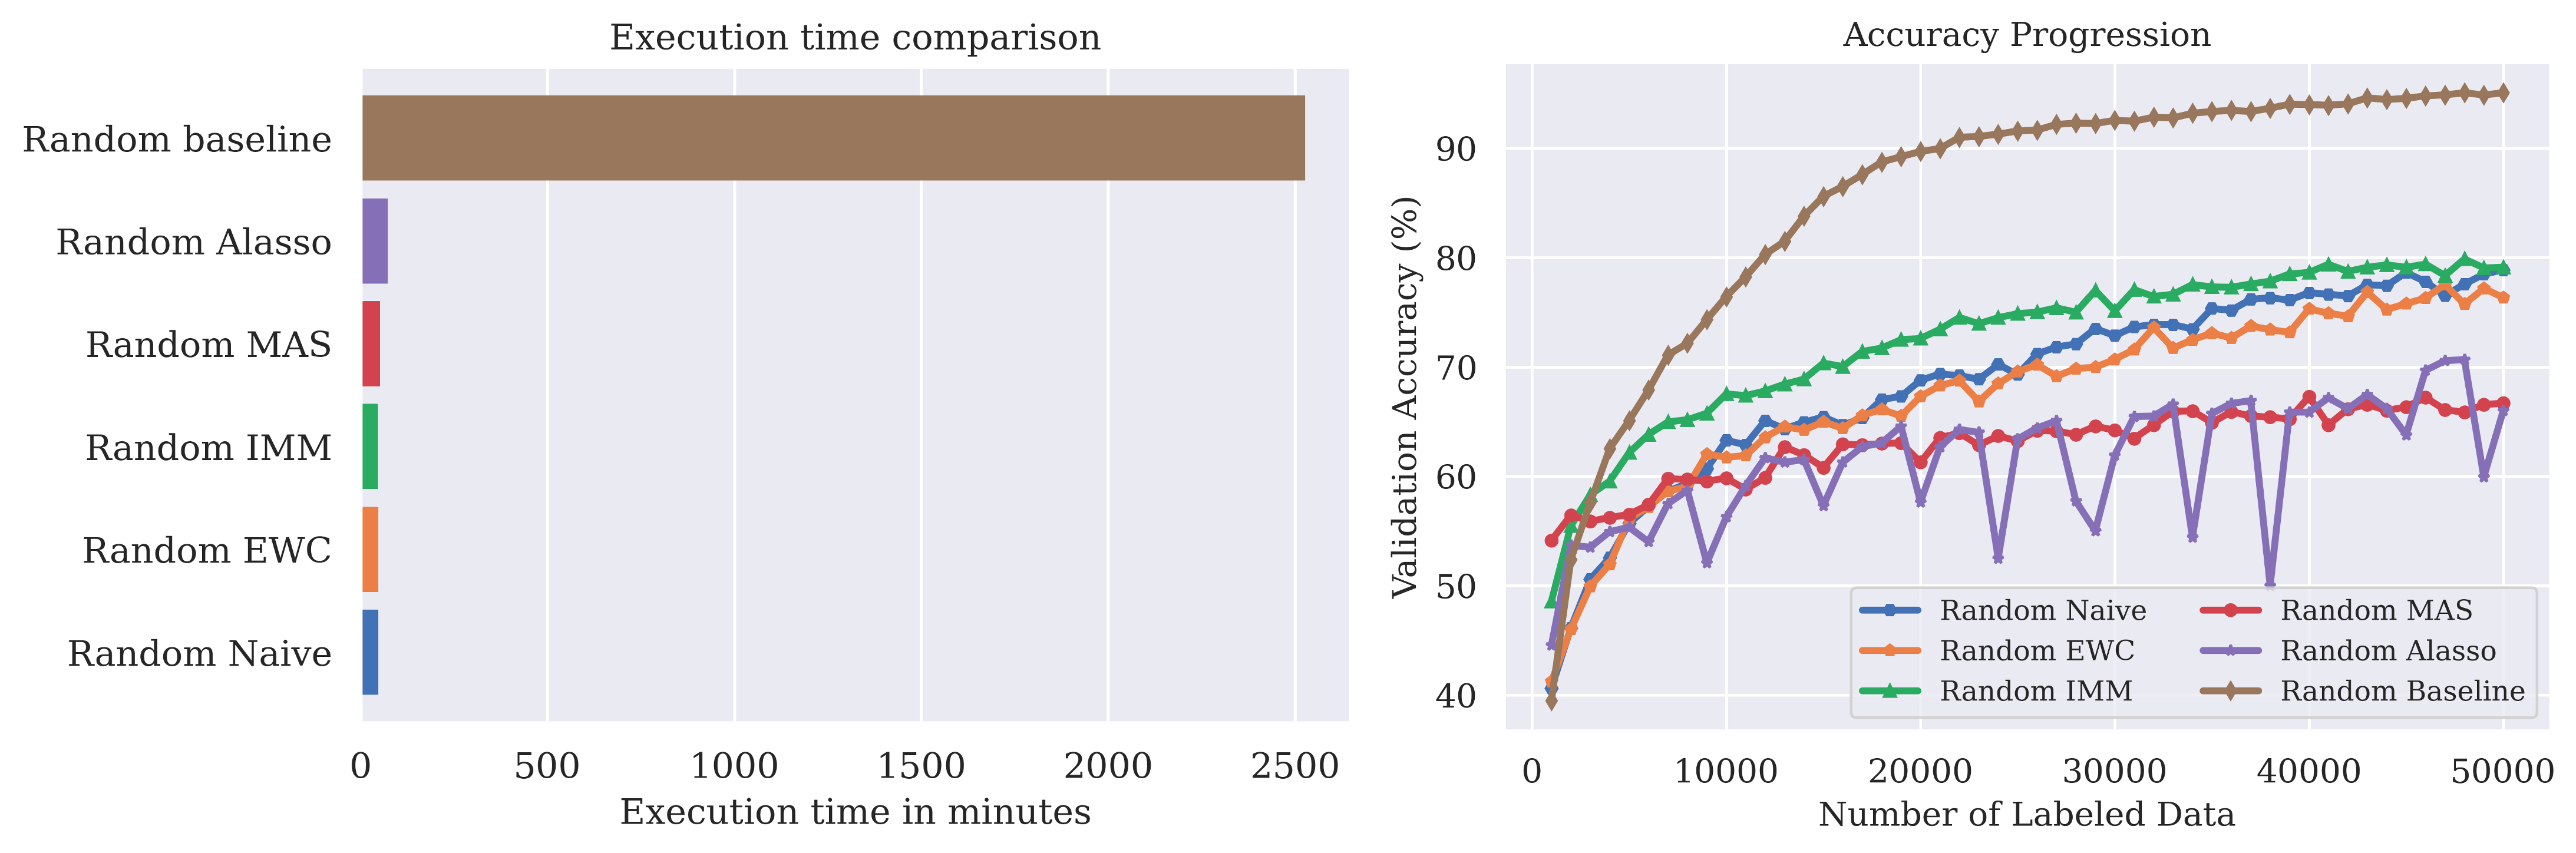
\includegraphics[width=\linewidth]{images/results_CAL/Random_CAL_1000b.png}
    \caption[Continual Active Learning Random 1000 batch size]{Comparison of execution time and validation accuracy of Continual Learning strategies used with the Active Learning strategy random.
    We use a batch size of 1000 for the experiments.}
    \label{fig:Evaluation:Results:CAL:Random1000}
\end{figure}

Next, we run the same experiment setup with the Active Learning strategy \gls{lc}. Results can be found in figure \ref{fig:Evaluation:Results:CAL:LC1000}. Again, all Continual Learning strategies
are significantly outperform the baseline in terms of execution time. \gls{alasso} is the slowest Continual Learning strategy, albeit being roughly 25 times faster than the baseline. The remaining Continual
Learning strategies, \gls{imm}, \gls{mas}, CoreSet and \gls{ewc}, are all about 50 times faster than the baseline. The gap in validation accuracy between Active Learning and all Continual Active Learning strategies
remains similar to the gap observed with Random. \gls{imm} and Naive perform similarly, outperforming the remaining Continual Learning strategies in the first half of the experiment. \gls{ewc} picks up on their
performance in the after 25000 sampled data. \gls{mas} and \gls{alasso} fall behind in terms of performance, with \gls{alasso} experiencing significant accuracy drops. \gls{mas}' validation accuracy remain stable throughout
the whole experiment, catching up to the other Continual Learning strategies in the end. \par

\begin{figure} [h]
    \centering
    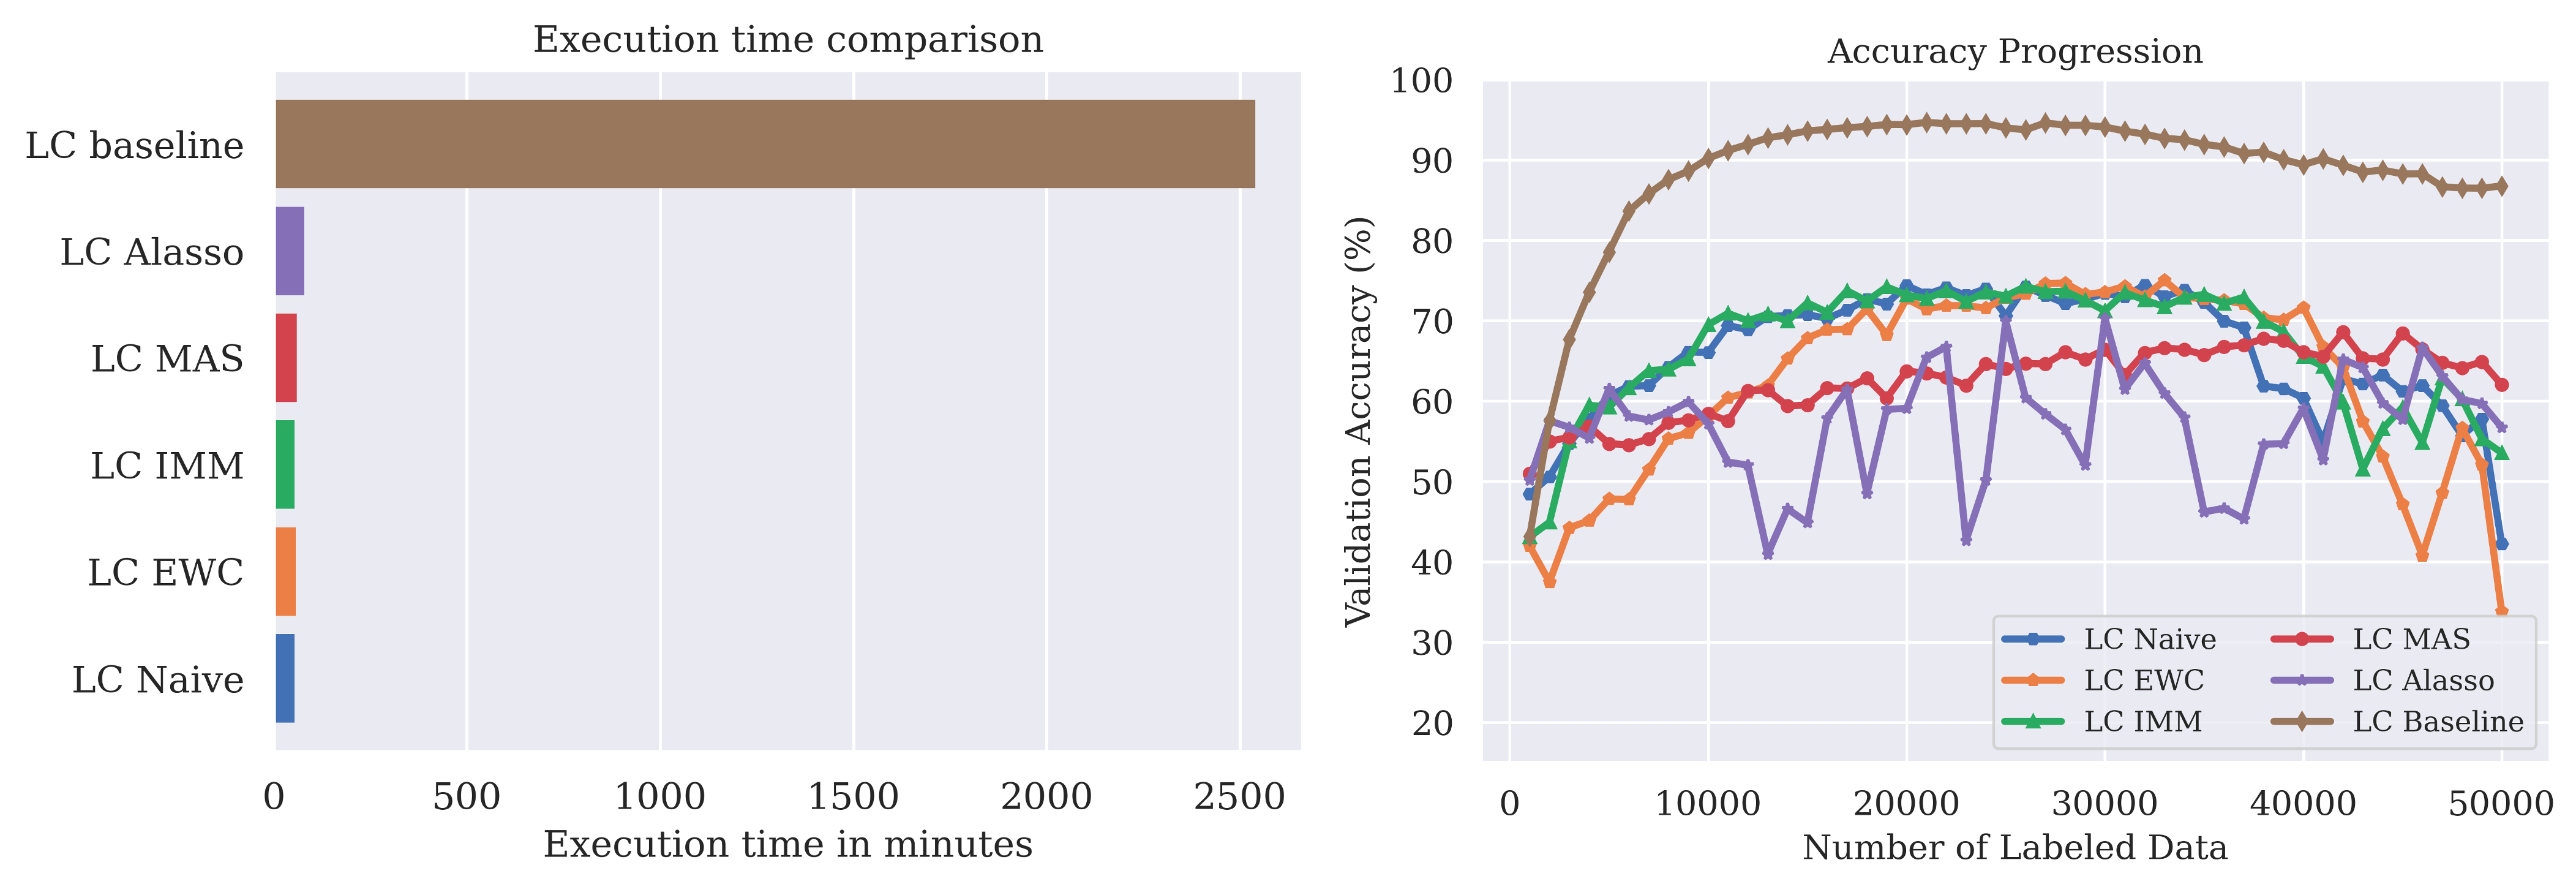
\includegraphics[width=\linewidth]{images/results_CAL/LC_CAL_1000b.png}
    \caption[Continual Active Learning \gls{lc} 1000 batch size]{Comparison of execution time and validation accuracy of Continual Learning strategies used with the Active Learning strategy \gls{lc}.
    We use a batch size of 1000 for the experiments.}
    \label{fig:Evaluation:Results:CAL:LC1000}
\end{figure}

\gls{bald} is the third Active Learning strategy we evaluate. Again, we use the same experiments setup as in the previous two experiments, changing only the Active Learning strategy but leaving every-
thing else as-is. The results of these experiments can be found in figure \ref{fig:Evaluation:Results:CAL:BALD1000}. In terms of runtime, the pattern established using \gls{lc} and Random continues.
\gls{mas}, \gls{imm}, \gls{ewc} and Naive are approximately 50 times as fast as the baseline, while \gls{alasso} is about 25 times as fast. Considering validation accuracy, all Continual Learning strategies perform significantly
worse than the baseline. Establishing a ranking between the Continual Learning strategies is difficult however, because they are all very erratic. \gls{alasso} stands out with the best and worst validation
accuracy, depending on the number of labeled samples. \gls{imm}, \gls{mas}, Naive and \gls{ewc} all have similar validaiton accuracy curves, although they are less erratic than \gls{alasso}. \par

\begin{figure}[h]
    \centering
    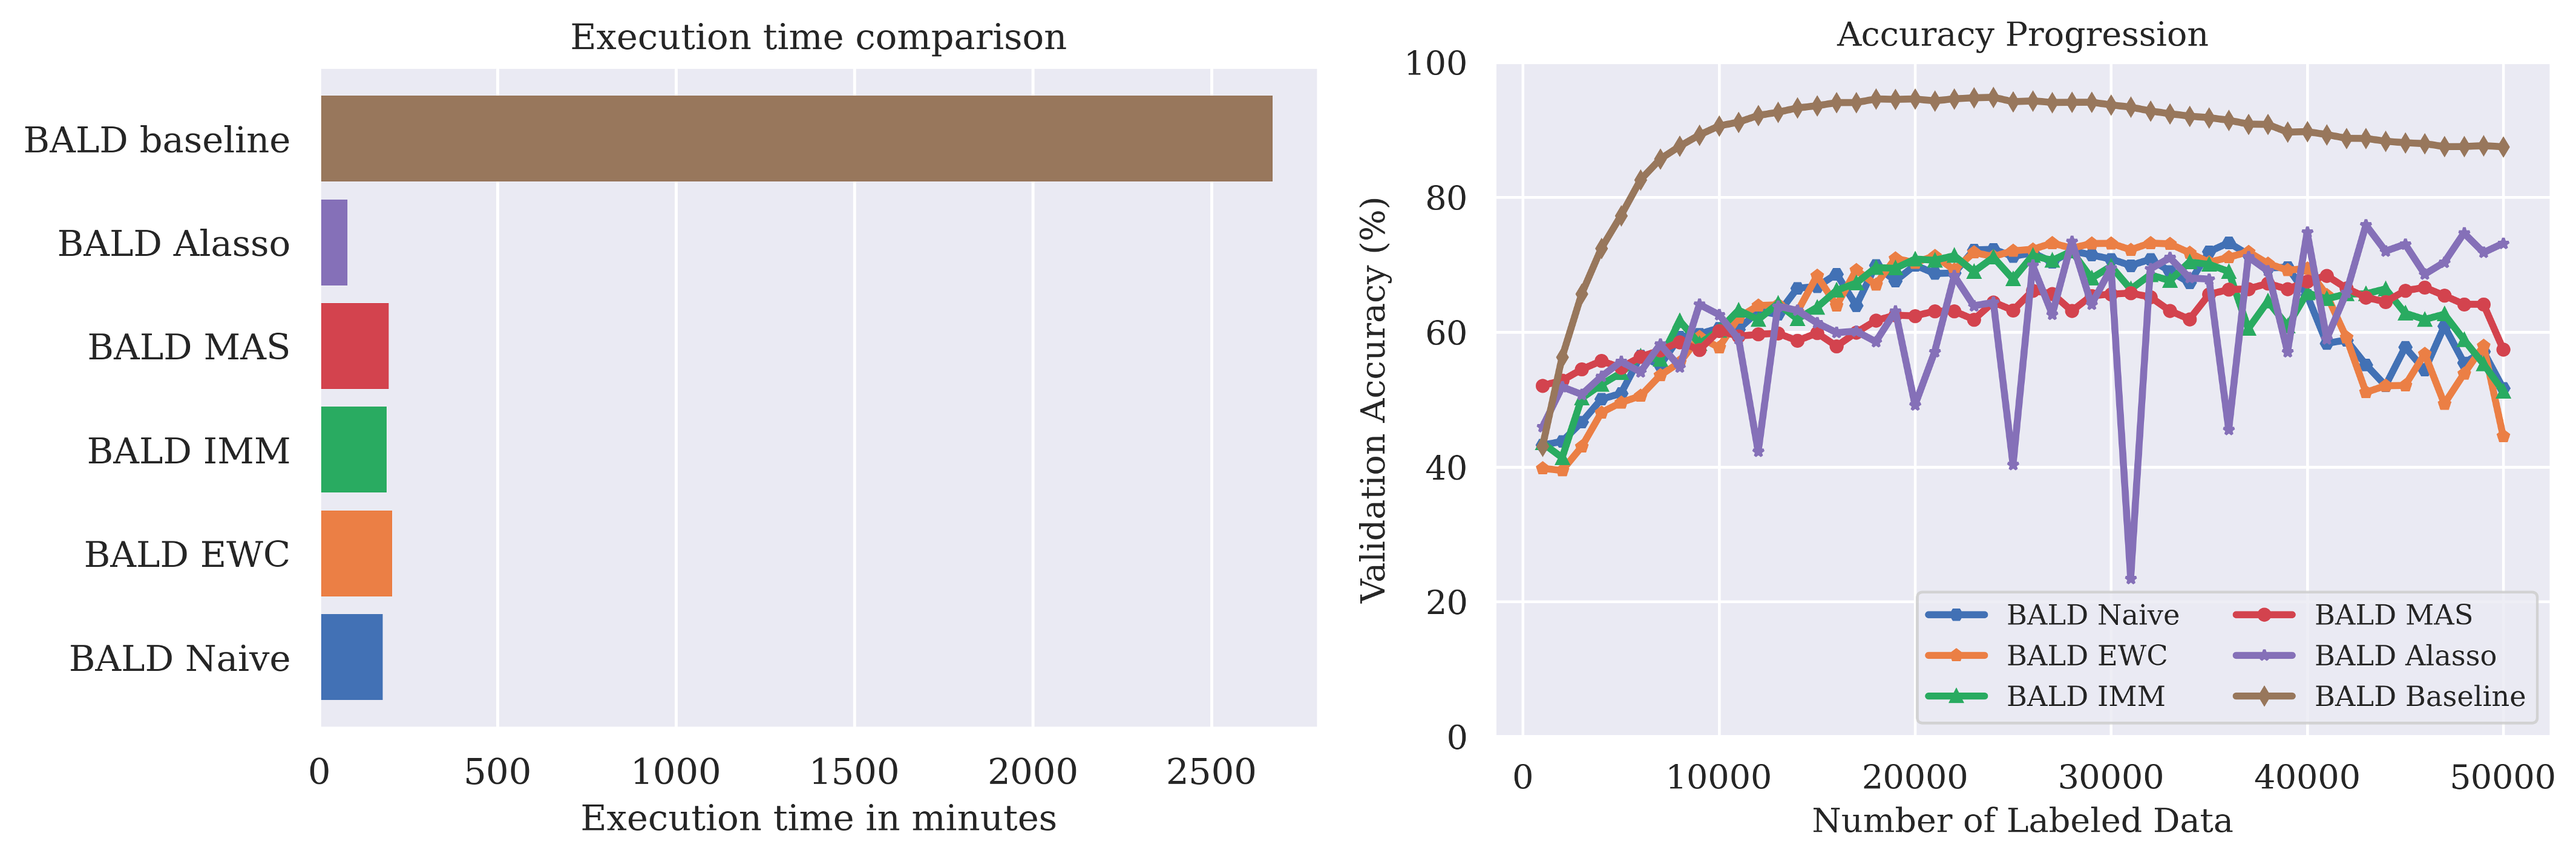
\includegraphics[width=\linewidth]{images/results_CAL/Bald_CAL_1000b.png}
    \caption[Continual Active Learning \gls{bald} 1000 batch size]{Comparison of execution time and validation accuracy of Continual Learning strategies used with the Active Learning strategy \gls{bald}.
    We use a batch size of 1000 for the experiments.}
    \label{fig:Evaluation:Results:CAL:BALD1000}
\end{figure}

After running our experiment with \gls{bald}, we re-run it using the Active Learning strategy CoreSet. We present the results in figure \ref{fig:Evaluation:Results:CAL:CoreSet1000}. The runtime of the 
Continual Learning strategies is again significantly lower than that of the baseline, however it is higher than in the previous experiments. \gls{alasso} is the slowest Continual Learning strategy, being
around 12 times as fast as the baseline. \gls{imm}, \gls{mas}, \gls{ewc} and Naive have a similar execution time and are approximately 15 times as fast as Active Learning using CoreSet. Just as in the previous experiments,
there is a significant gap in validation accuracy between the baseline and all Continual Learning strategies. \gls{imm}, \gls{ewc} and Naive perform almost similarly while \gls{mas} and \gls{alasso} fall behind. While \gls{mas} demon-
strates a marginally increasing validation accuracy, the validation accuracy curve of \gls{alasso} is unstable with significant drops and jumps in accuracy as the number of labeled data increases. \par

\begin{figure}[h]
    \centering
    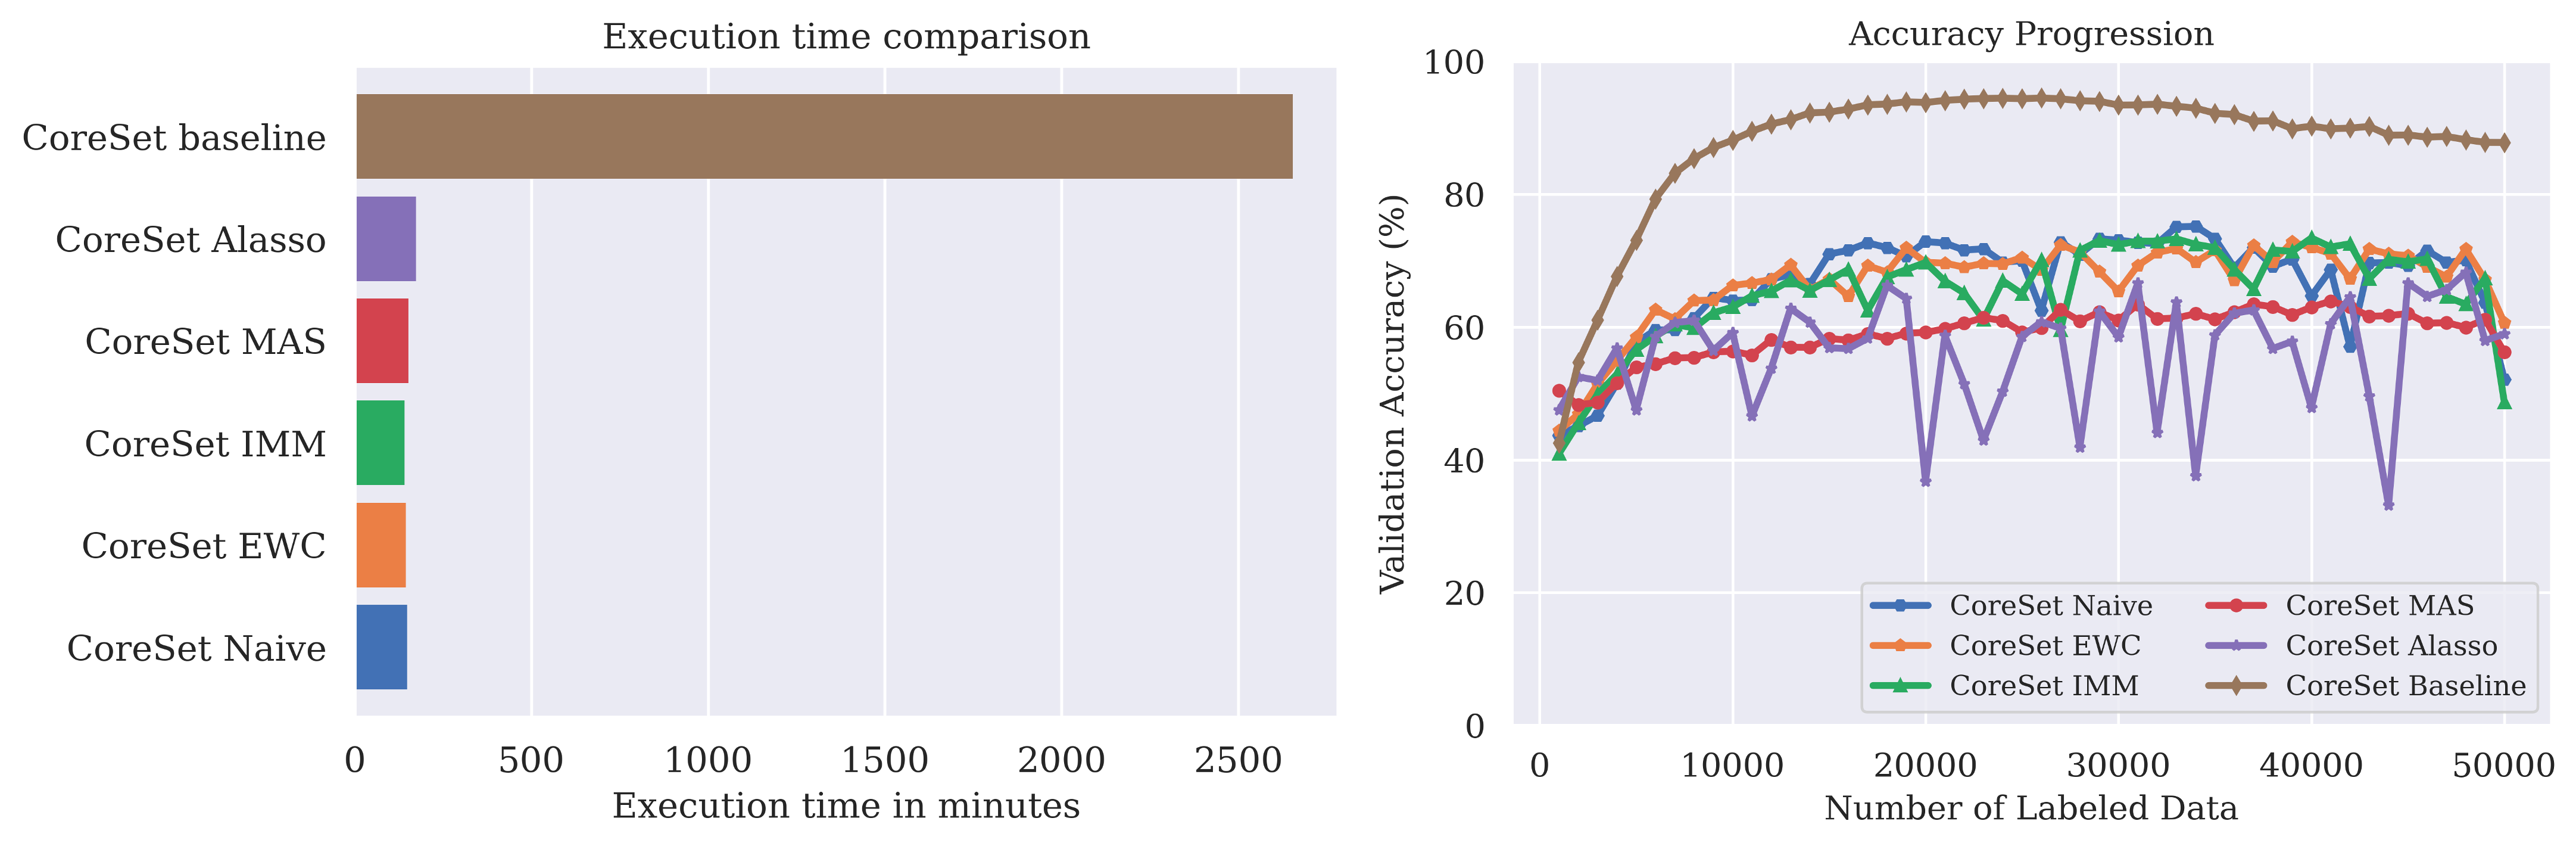
\includegraphics[width=\linewidth]{images/results_CAL/CoreSet_CAL_1000b.png}
    \caption[Continual Active Learning CoreSet 1000 batch size]{Comparison of execution time and validation accuracy of Continual Learning strategies used with the Active Learning strategy
     CoreSet. We use a batch size of 1000 for the experiments. }
    \label{fig:Evaluation:Results:CAL:CoreSet1000}
\end{figure}

In our final experiment with batch size 1000, we use the Active Learning strategy \gls{badge}. The results are shown in figure \ref{fig:Evaluation:Results:CAL:Badge1000}. All Continual Learning strategies
outperform the baseline in terms of runtime by a large margin. Between the Continual Learning strategies, there are only marginal differences in execution time. The validation accuracy of all Continual
Learning strategies is irregular and all of them leave a significant gap to the baseline. There is no Continual Learning strategy which demonstrates a significantly higher or lower validation accuracy
than the others. However, \gls{mas} and \gls{alasso} fall behind the other Continual Learning strategies at around 25000 samples but manage to catch up in the end. \par

\begin{figure}[h]
    \centering
    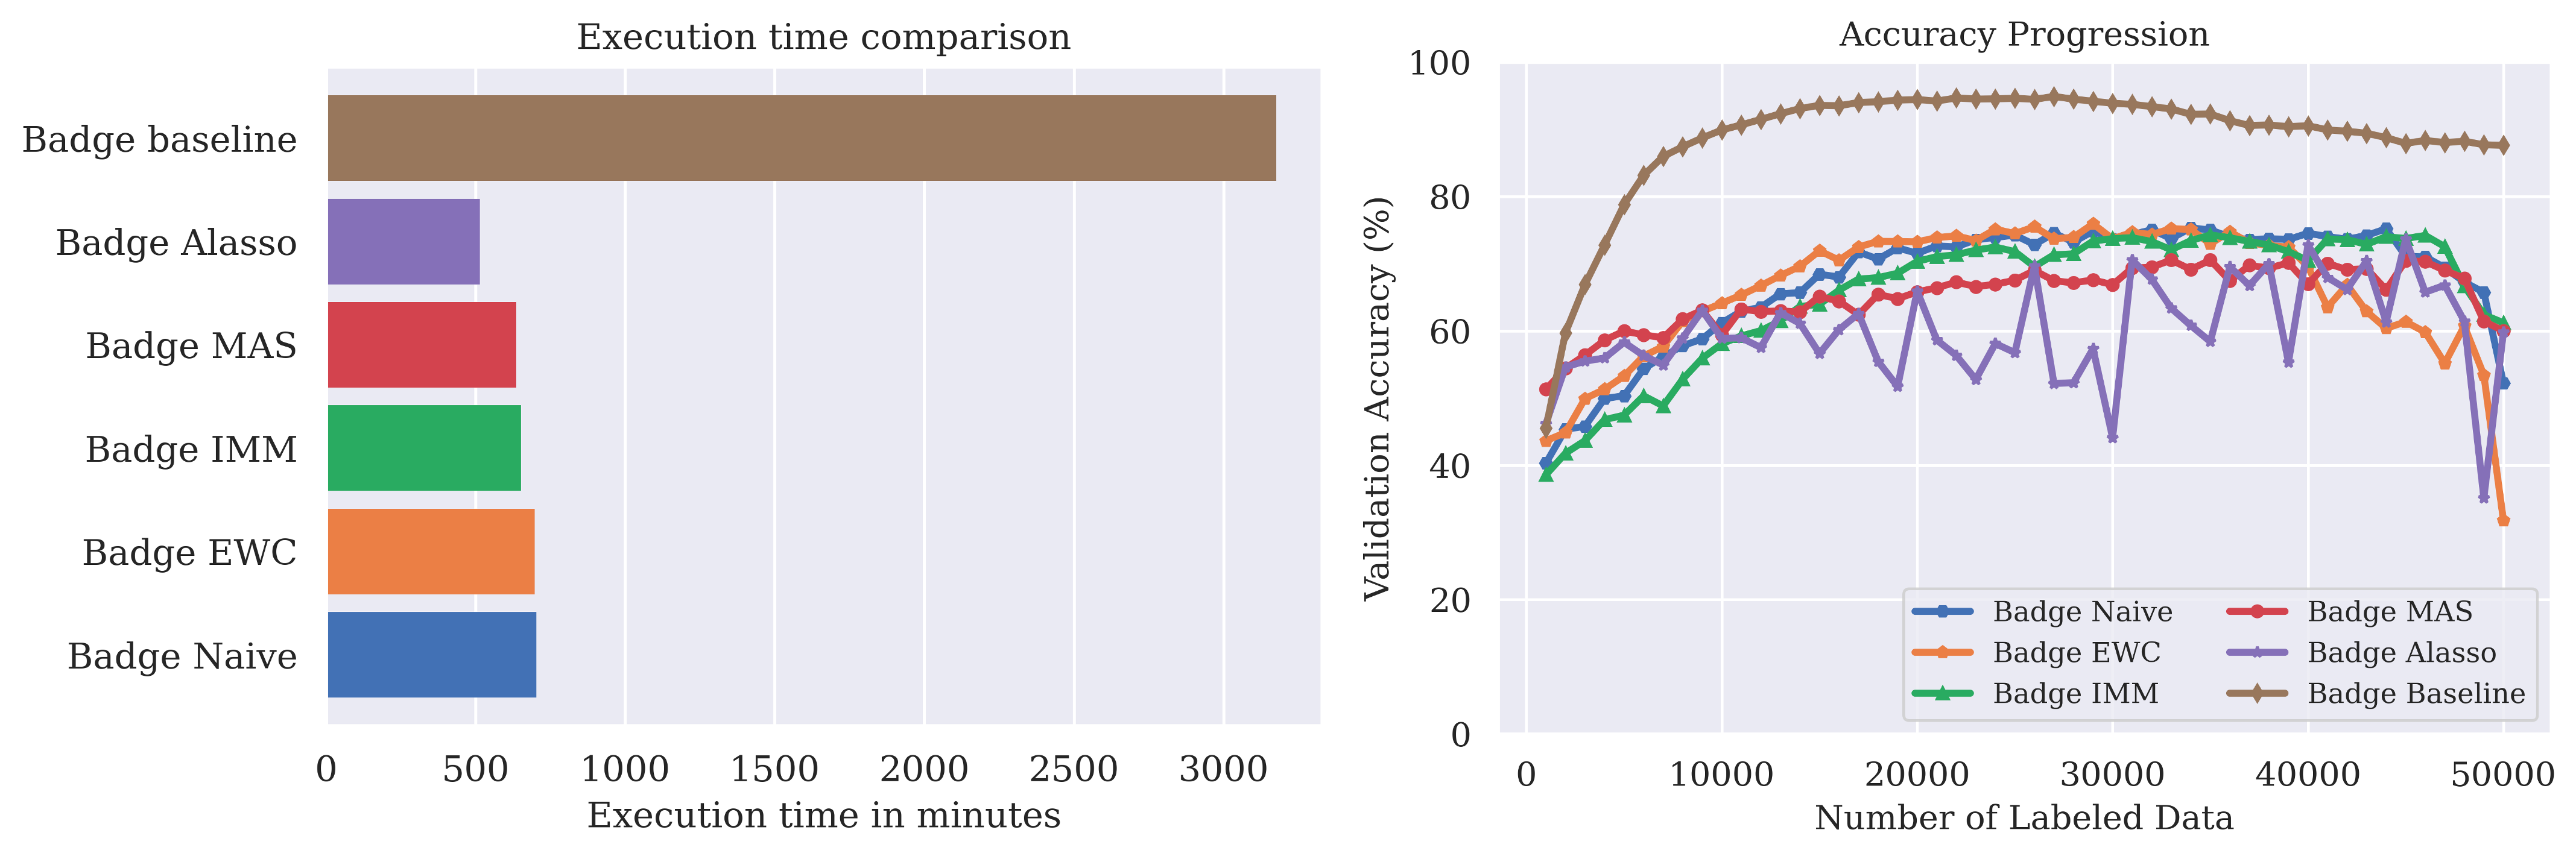
\includegraphics[width=\linewidth]{images/results_CAL/Badge_CAL_1000b.png}
    \caption[Continual Active Learning \gls{badge} 1000 batch size]{Comparison of execution time and validation accuracy of Continual Learning strategies used with the Active Learning strategy
    \gls{badge}. We use a batch size of 1000 for the experiments. }
    \label{fig:Evaluation:Results:CAL:Badge1000}
\end{figure}

After running the experiment with \gls{badge}, CoreSet, \gls{lc}, \gls{bald} and Random, we perform the same experiment with Random but increase the batch size from 1000 to 2000. We present the results in
Figure \ref{fig:Evaluation:Results:CAL:Random2000}. The execution time remains significantly lower for all Continual Learning strategies compared to the baseline, however, the gap has decreased. 
\gls{alasso} is the slowest Continual Learning Strategy, being about 8 times as fast as the baseline. \gls{mas}, \gls{imm}, \gls{ewc} and Naive have similar execution times, being about 10 times as fast as the baseline. 
The gap in validation accuracy between the baseline and the Continual Learning strategies is still significant, however, it has decreased compared the experiment with a batch size of 1000.
\gls{ewc} outperforms all Continual Learning strategies, including Naive, although the gap between the two is marginal. \gls{alasso}, \gls{imm} and \gls{mas} perform show similar overall performance although the course
of their validation accuracy curves differ greatly. \gls{imm} starts worst and ends best. \gls{mas} shows similar performance to \gls{alasso} but is outperformed within the final 5000 samples. \par

\begin{figure}[h]
    \centering
    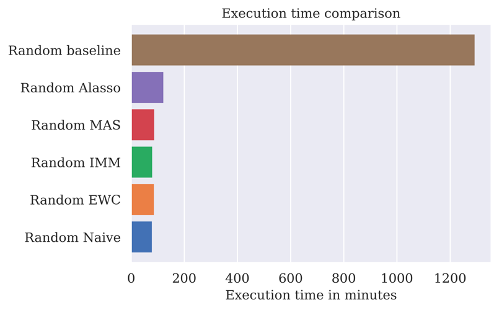
\includegraphics[width=\linewidth]{images/results_CAL/Random_CAL_2000b.png}
    \caption[Continual Active Learning Random 2000 batch size]{Comparison of execution time and validation accuracy of Continual Learning strategies used with the Active Learning strategy
    Random. We use a batch size of 2000 for the experiments.}
    \label{fig:Evaluation:Results:CAL:Random2000}
\end{figure}

Second, we run the experiment with batch size 2000 for the Active Learning strategy \gls{lc}. Our results can be found in figure \ref{fig:Evaluation:Results:CAL:LC2000}. Like in the previous experiment,
the gap in execution time between the baseline and the Continual Learning strategies has shrunk compared to the experiment with a batch size of 1000. Again, \gls{alasso} is the slowest Continual Learning
strategy, being approximately 9 times as fast as the baseline. \gls{ewc} is the second slowest strategy, being only marginally slower than \gls{mas}, \gls{imm} and Naive, who have a very similar execution time.
In terms of validation accuracy, there is still a significant gap between the baseline and the Continual Learning strategies. \gls{imm}, \gls{ewc} and Naive perform similar for the first 35000 samples, outperforming
\gls{mas} and \gls{alasso}. In the final 15000 samples, all \gls{imm}, \gls{ewc} and Naive experience a drop in validation accuracy, which is most significant for \gls{ewc}. The accuracy of \gls{mas} increases modestly until the labeled
pool contains 40000 samples, before dropping of by about 10\%. The validation accuracy curve of \gls{alasso} is again unstable, showing a slight downward trend over the course of the experiment. \par

\begin{figure}[h]
    \centering
    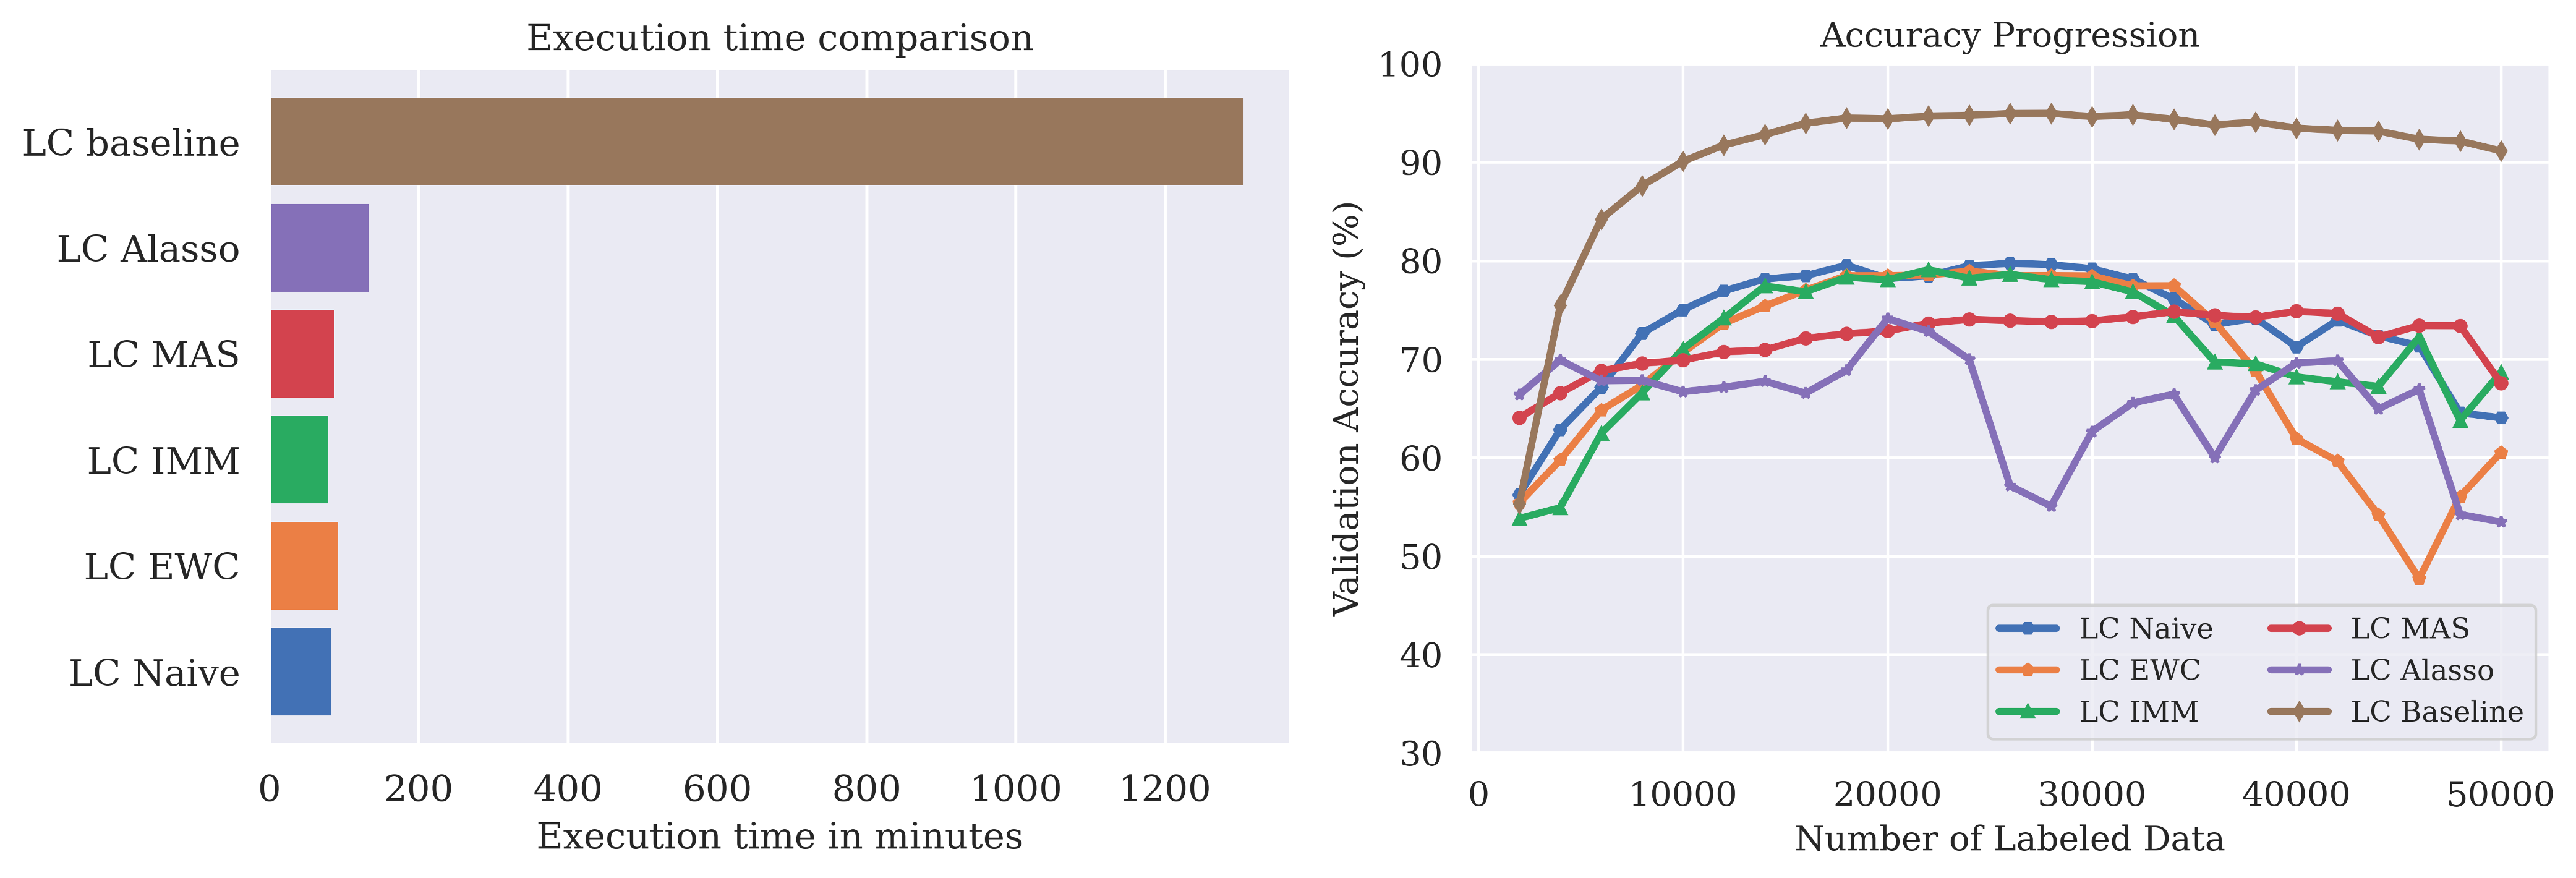
\includegraphics[width=\linewidth]{images/results_CAL/LC_CAL_2000b.png}
    \caption[Continual Active Learning \gls{lc} 2000 batch size]{Comparison of execution time and validation accuracy of Continual Learning strategies used with the Active Learning strategy
    \gls{lc}. We use a batch size of 2000 for the experiments.}
    \label{fig:Evaluation:Results:CAL:LC2000}
\end{figure}

We follow up with the experiment using the Active Learning strategy \gls{bald}, all other parameters being equal. The results can be found in figure \ref{fig:Evaluation:Results:CAL:BALD2000}. The gap in
execution time between the baseline and the Continual Learning strategies has declined compared to the experiment with \gls{bald} and batch size 1000. Naive and \gls{imm} are the fastest Continual Learning strategies,
closely followed \gls{ewc} and \gls{mas}. \gls{alasso} follows last, but is still about 10 times as fast as the baseline. The validation accuracy curves of most Continual Learning strategies are similar, with \gls{alasso} falling 
out of line. \gls{ewc}, \gls{imm} and Naive perform similar across the whole experiment with \gls{mas} starting off better but falling behind after approximately 15000 samples. \gls{alasso} performs on par with the remaining strategies
at first, but suffers from a heavy decrease in validation accuracy at around 15000 samples. All Continual Learning strategies leave a large gap to the baseline in terms of validation accuracy. \par

\begin{figure}[h]
    \centering
    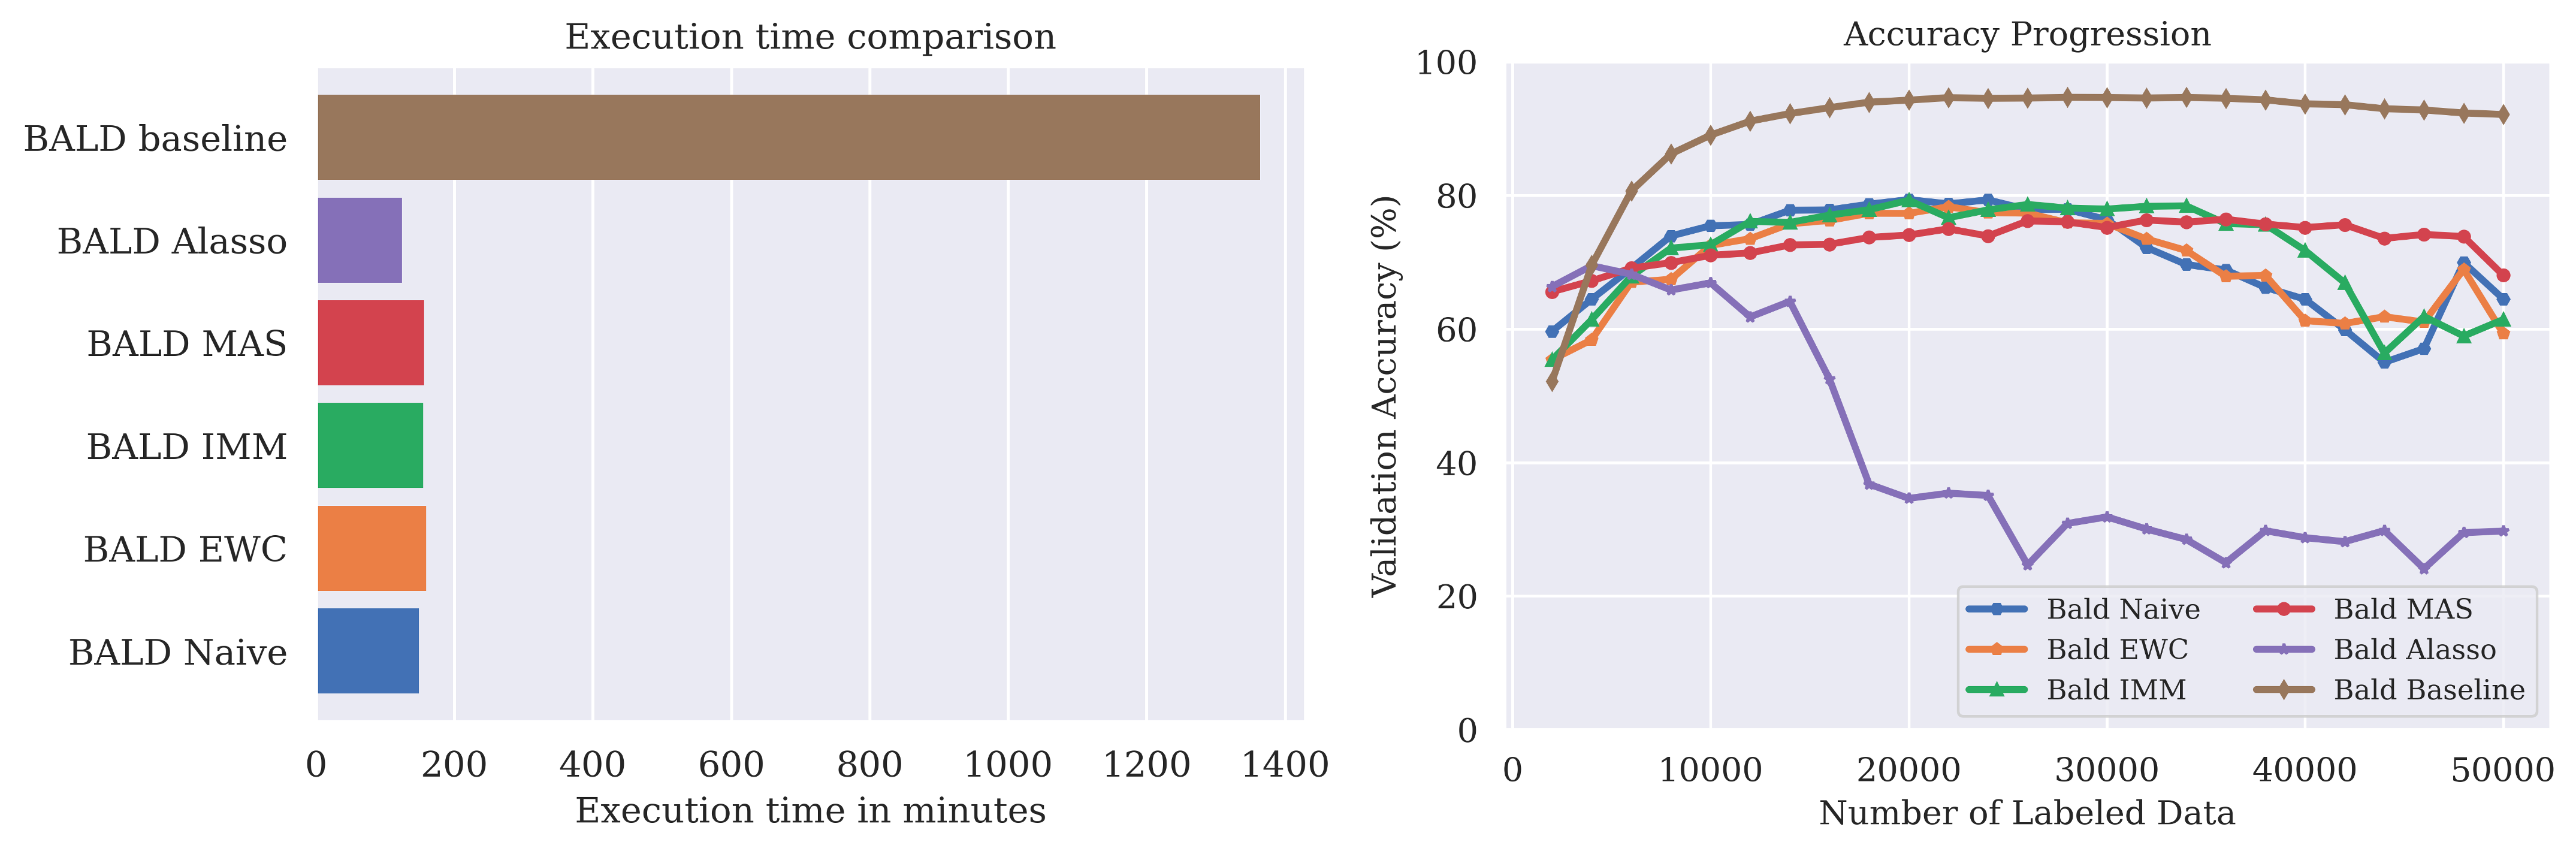
\includegraphics[width=\linewidth]{images/results_CAL/Bald_CAL_2000b.png}
    \caption[Continual Active Learning \gls{bald} 2000 batch size]{Comparison of execution time and validation accuracy of Continual Learning strategies used with the Active Learning strategy
    \gls{bald}. We use a batch size of 2000 for the experiments.}
    \label{fig:Evaluation:Results:CAL:BALD2000}
\end{figure}

Next, we run the experiment with CoreSet and a batch size of 2000. We present our results in figure \ref{fig:Evaluation:Results:CAL:CoreSet2000}. The gap in execution time between the baseline and the
Continual Learning strategies has again decreased. \gls{imm} is the fastest Continual Learning strategy, closely followed by \gls{ewc}. \gls{ewc} is followed by Naive and \gls{mas}, who have similar execution times. \gls{alasso} is
the slowest approach, albeit being about 6.5 times as fast as the baseline. Regarding validation accuracy, all Continual Learning strategies are significantly outperformed by the baseline. Naive performs best
in the first half of the experiment, followed by \gls{ewc}, \gls{imm} and \gls{mas}. At around 25000 samples, the validation accuracy of \gls{imm}, \gls{ewc} and Naive suddenly becomes erratic, followed by a moderate increase in validation
accuracy and a drop in the final 10000 samples. \gls{mas} performs consistent but worse than \gls{imm}, \gls{ewc} and Naive, experiencing a moderate drop in validation accuracy in the final 10000 samples. \gls{alasso} performs worst,
with its validation accuracy decreasing over the course of the experiment. \par

\begin{figure}[h]
    \centering
    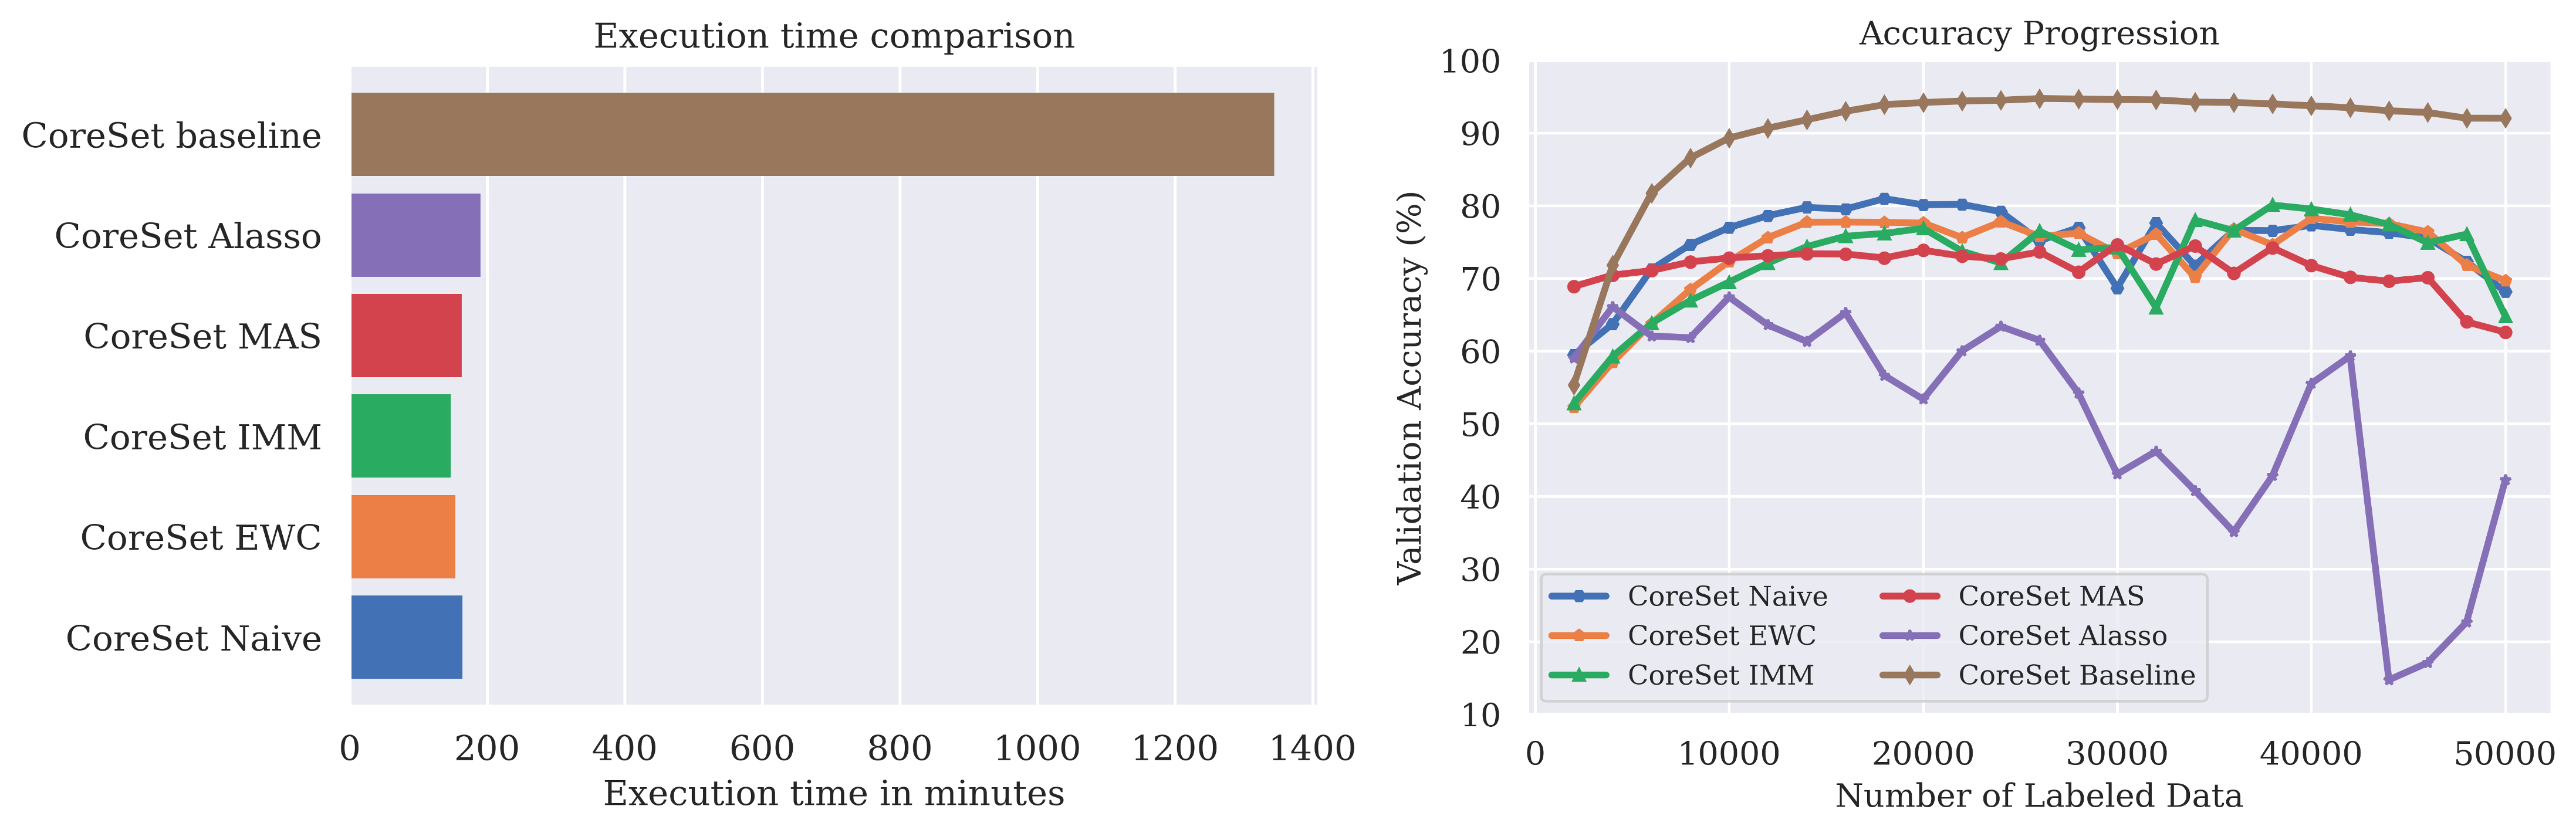
\includegraphics[width=\linewidth]{images/results_CAL/CoreSet_CAL_2000b.png}
    \caption[Continual Active Learning CoreSet 2000 batch size]{Comparison of execution time and validation accuracy of Continual Learning strategies used with the Active Learning strategy
    CoreSet. We use a batch size of 2000 for the experiments.}
    \label{fig:Evaluation:Results:CAL:CoreSet2000}
\end{figure}

Finally, we run the same experiment with the Active Learning strategy \gls{badge}. Our results can be found in figure \ref{fig:Evaluation:Results:CAL:Badge2000}. The margin in execution time between the baseline
and the Continual Learning strategies has decreased which is mainly due to the large decrease in runtime of the baseline, compared to the experiment with 1000 batch size. Nevertheless, the Continual
Learning strategies are about 3.5 times as fast as the baseline. Within the Continual Learning strategies there is only a minor runtime difference, with \gls{imm} being the fastest and \gls{alasso} the slowest. In terms of 
validation accuracy, the gap between the baseline as the Continual Learning strategies has decreased. More notably though, the validation accuracy curves of all Continual Learning strategies more consistent than
in the previous experiment with 1000 batch size. \gls{imm}, \gls{ewc} and Naive perform similar, followed by \gls{mas}. \gls{alasso} is the worst performing strategy, falling behind the others after bout 10000 samples. \par

\begin{figure}[h]
    \centering
    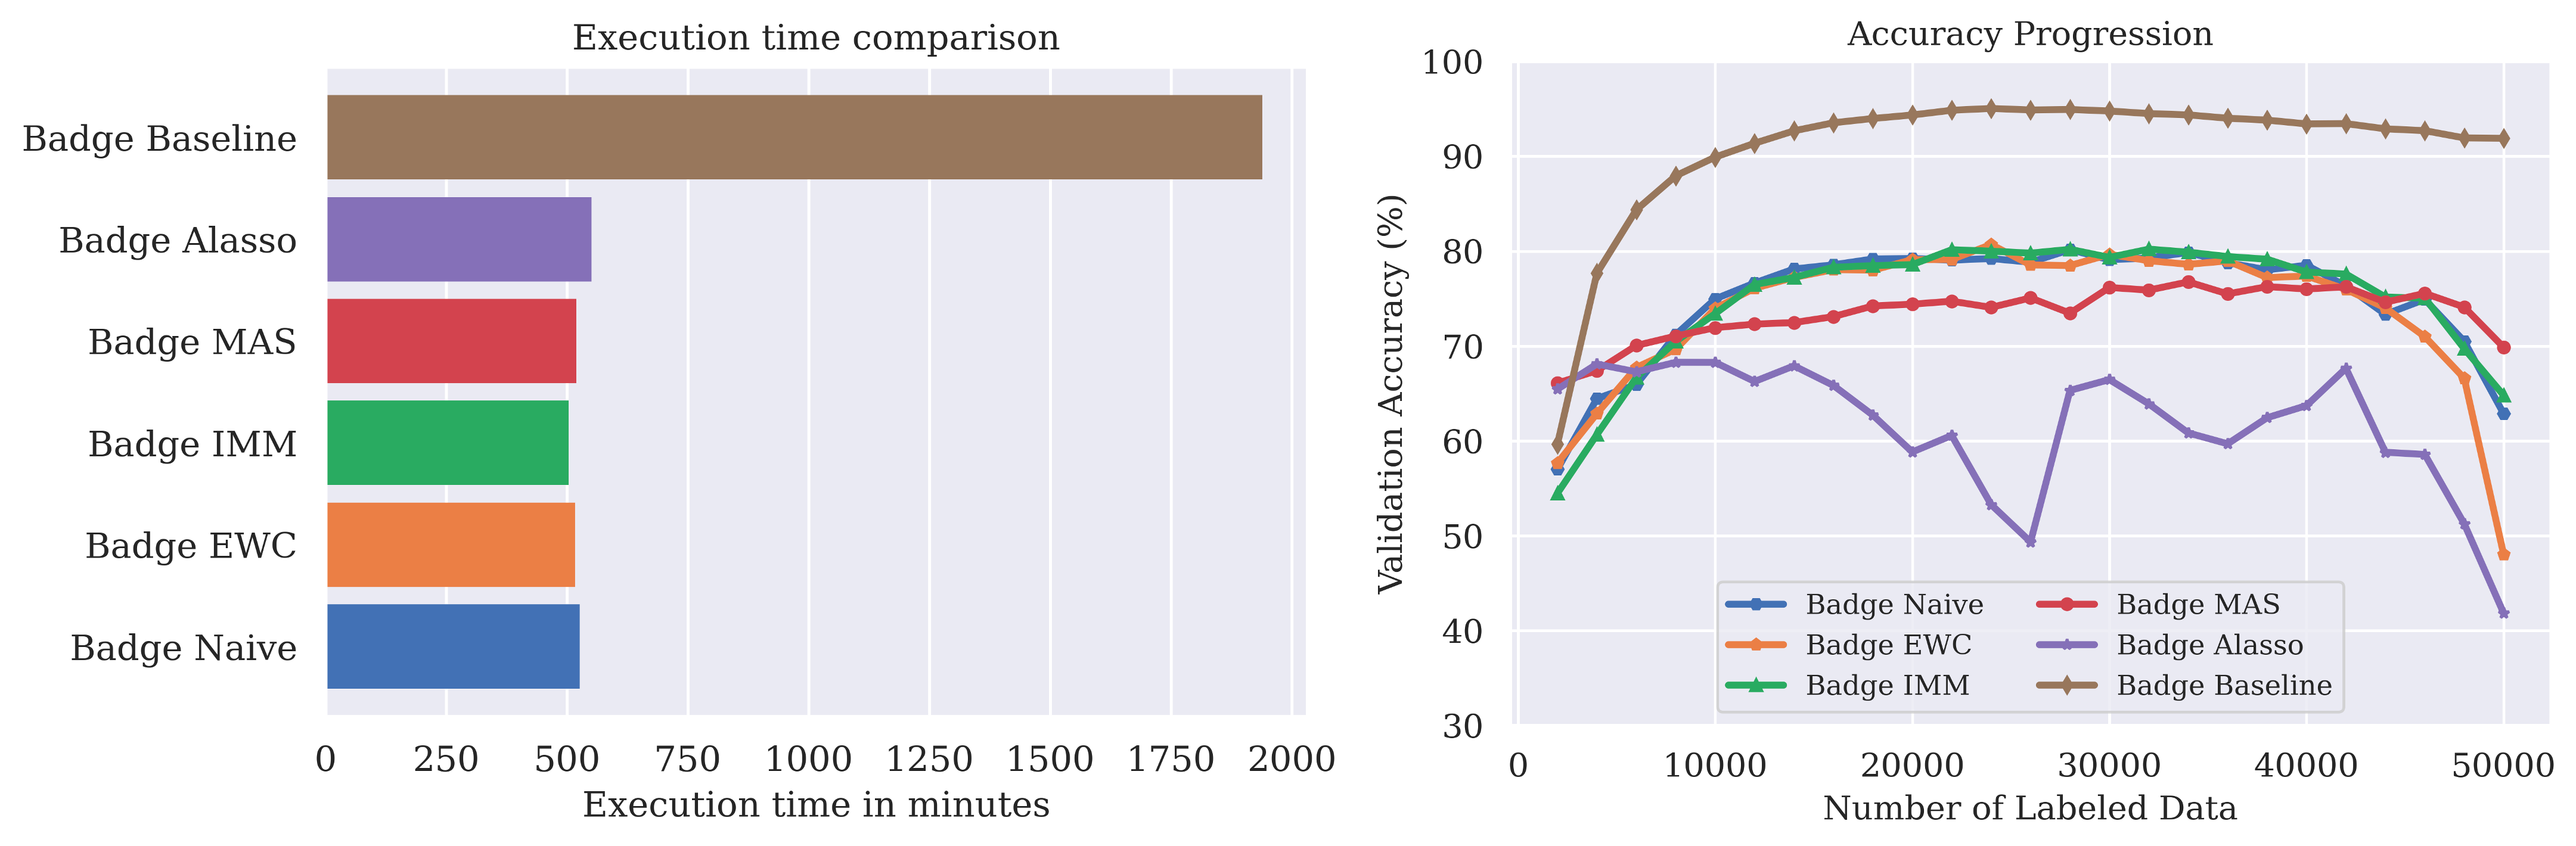
\includegraphics[width=\linewidth]{images/results_CAL/Badge_CAL_2000b.png}
    \caption[Continual Active Learning \gls{badge} 2000 batch size]{Comparison of execution time and validation accuracy of Continual Learning strategies used with the Active Learning strategy
    \gls{badge}. We use a batch size of 2000 for the experiments.}
    \label{fig:Evaluation:Results:CAL:Badge2000}
\end{figure}

Motivated by the increase in validation accuracy of the Continual Learning strategies with increasing batch size, we decide to re-run the experiments with a batch size of 4000. We start with the Active Learning
strategy Random. The results can be found in figure \ref{fig:Evaluation:Results:CAL:Random4000}. The gap in execution time between the baseline and the Continual Learning strategies has further decreased. \gls{imm} is
the fastest strategy, followed by \gls{mas}, \gls{ewc} and Naive who perform on the same level in terms of execution time. \gls{alasso} is the slowest strategy, but is still about 6 times as fast as the baseline. There is still a
gap in validation accuracy between the baseline and the Continual Learning strategies, however it is smaller than in the experiment with batch size 2000. Overall, \gls{ewc} and Naive perform best, followed by \gls{imm} and \gls{mas}.
\gls{alasso} starts of as the best strategy but suffers from a heavy decrease in validation accuracy, starting at around 8000 samples. \par

\begin{figure}[h]
    \centering
    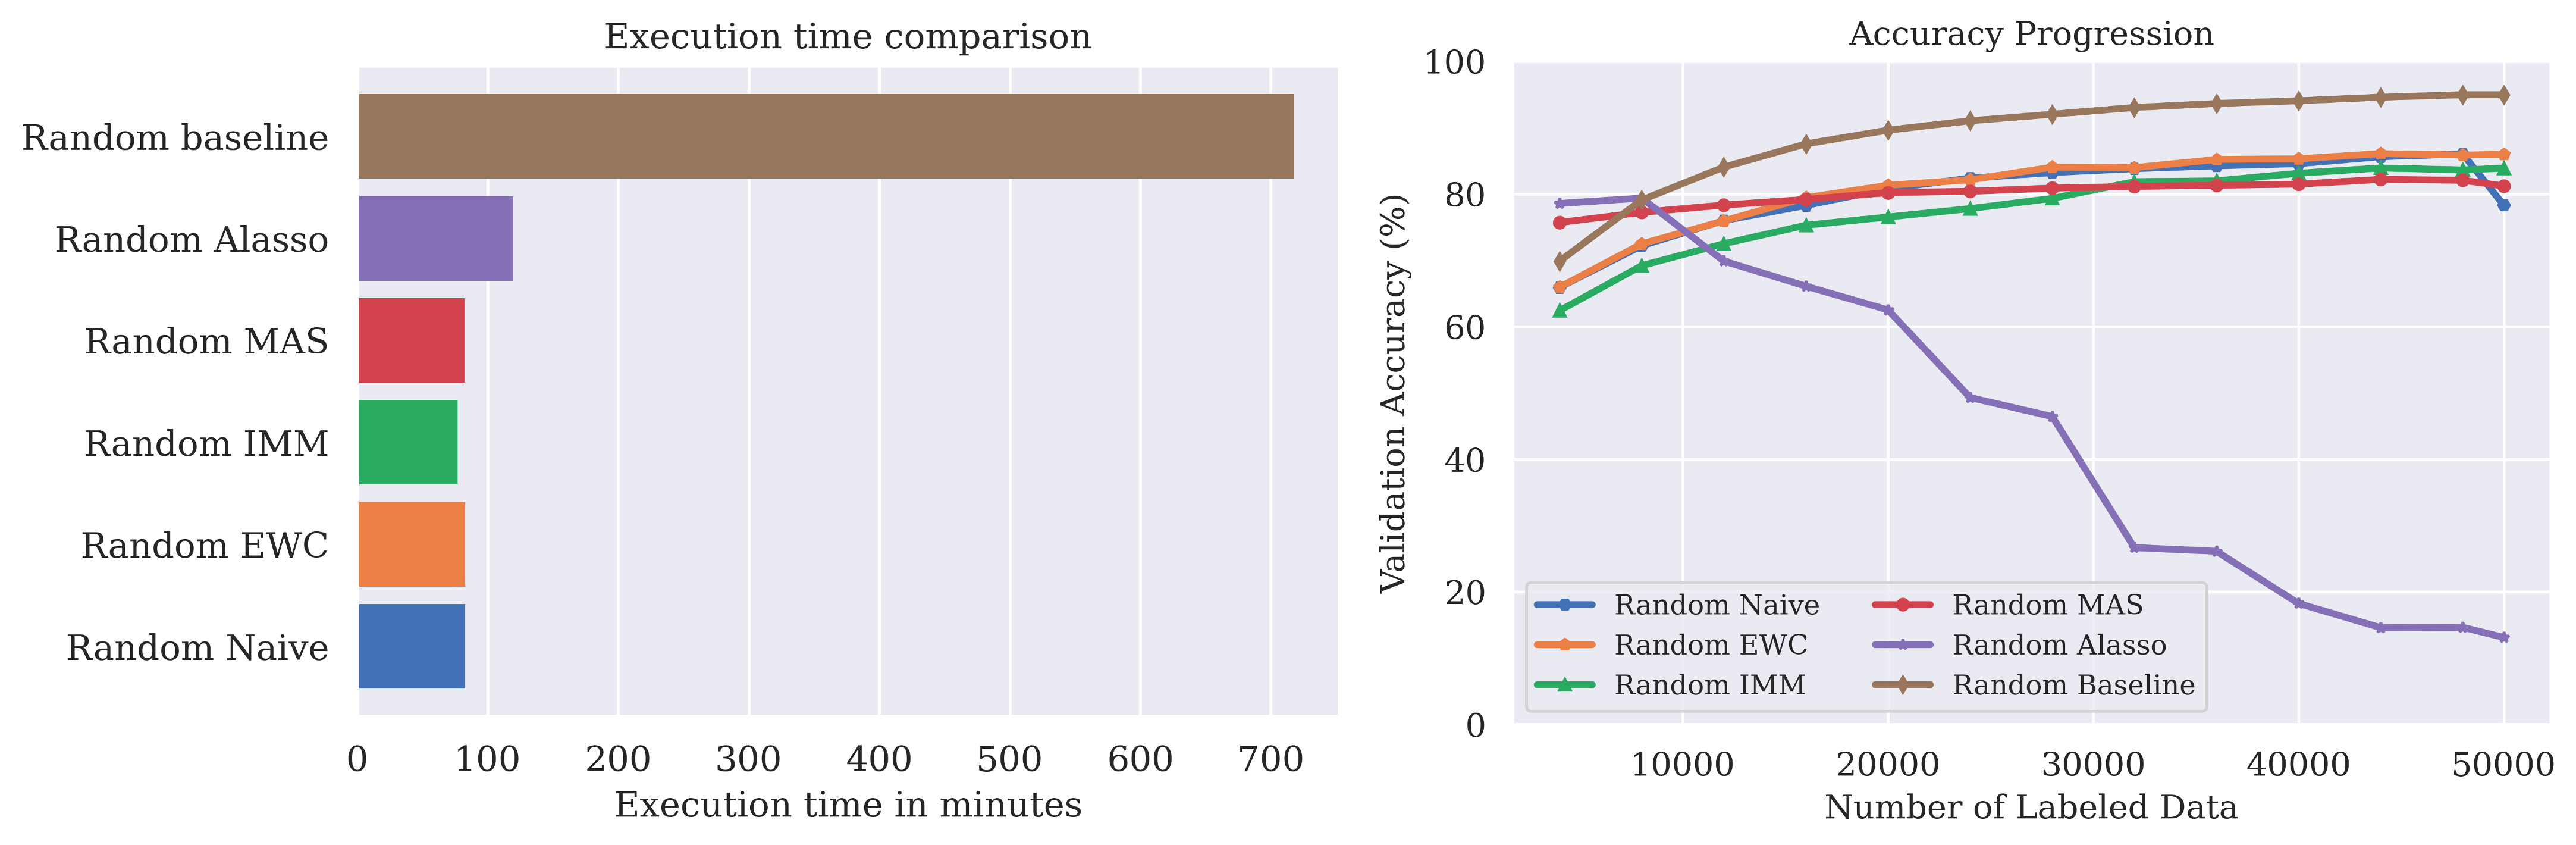
\includegraphics[width=\linewidth]{images/results_CAL/Random_CAL_4000b.png}
    \caption[Continual Active Learning Random 4000 batch size]{Comparison of execution time and validation accuracy of Continual Learning strategies used with the Active Learning strategy
    Random. We use a batch size of 4000 for the experiments}
    \label{fig:Evaluation:Results:CAL:Random4000}
\end{figure}

Next, we re-run the previous experiment with the Active Learning strategy \gls{lc}, again using a batch size of 4000. We present the results of the experiment in Figure \ref{fig:Evaluation:Results:CAL:LC4000}. In terms of runtime,
the results are similar to the experiment with Random, with \gls{alasso} being the slowest Continual Learning strategy, followed by \gls{mas}, \gls{ewc}, \gls{imm} and Naive. All Continual Learning strategies are significantly faster than the baseline,
with \gls{alasso} being about 6 times as fast and Naive about 10 times as fast. The gap in validation accuracy between the baseline and the Continual Learning strategies remains significant, although it has shrunk compared to the
experiment with 2000 batch size. \gls{imm}, \gls{ewc} and Naive perform almost identically across the experiment with \gls{mas} following closely and outperforming the remaining strategies within the last 5000 samples. \gls{alasso} starts of on par
with the remaining strategies, but suffers from a heavy decrease in validation accuracy at around 8000 samples. \par

\begin{figure}[h]
    \centering
    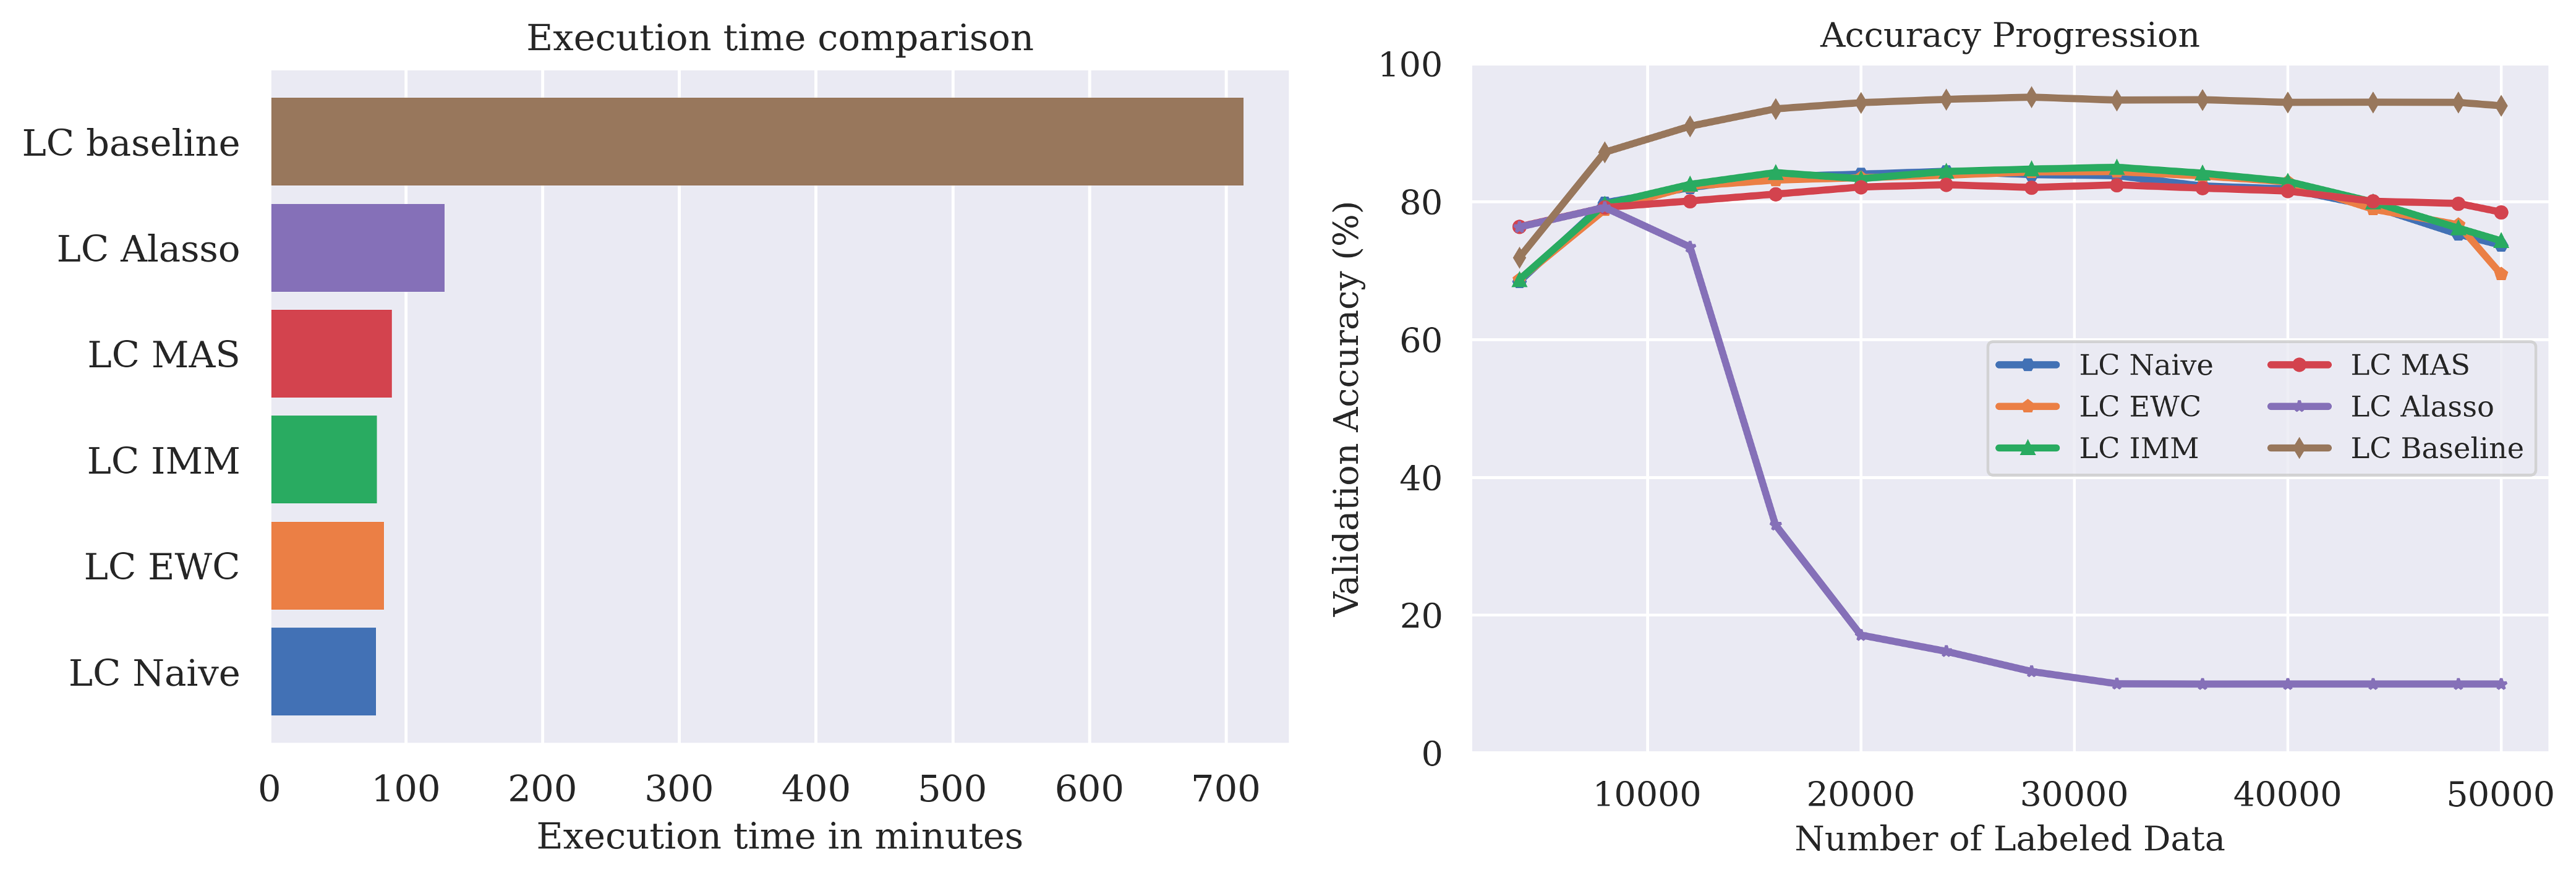
\includegraphics[width=\linewidth]{images/results_CAL/LC_CAL_4000b.png}
    \caption[Continual Active Learning \gls{lc} 4000 batch size]{Comparison of execution time and validation accuracy of Continual Learning strategies used with the Active Learning strategy
    \gls{lc}. We use a batch size of 4000 for the experiments. }
    \label{fig:Evaluation:Results:CAL:LC4000}
\end{figure}

The third experiment with a batch size of 4000 is run with the Active Learning strategy \gls{bald}. The results of the experiment can be found in figure \ref{fig:Evaluation:Results:CAL:BALD4000}. The ranking of execution time of the Continual
Learning strategies and the baseline is similar to the previous experiment with \gls{lc}. In terms of accuracy, there remains a large gap between the baseline and all Continual Learning strategies. Naive, \gls{imm} and \gls{ewc} perform similar, showing an
s-shaped validation accuracy curve. The performance of \gls{mas} follows a similar curve, however \gls{mas} performs better in the first half of the experiment, and worse in the second half compared to the three former strategies. \gls{alasso} starts off as
the best Continual Learning strategy, but its validation accuracy decreases steadily over the course of the experiment, until it suffers a huge drop in the final iteration. \par 

\begin{figure}[h]
    \centering
    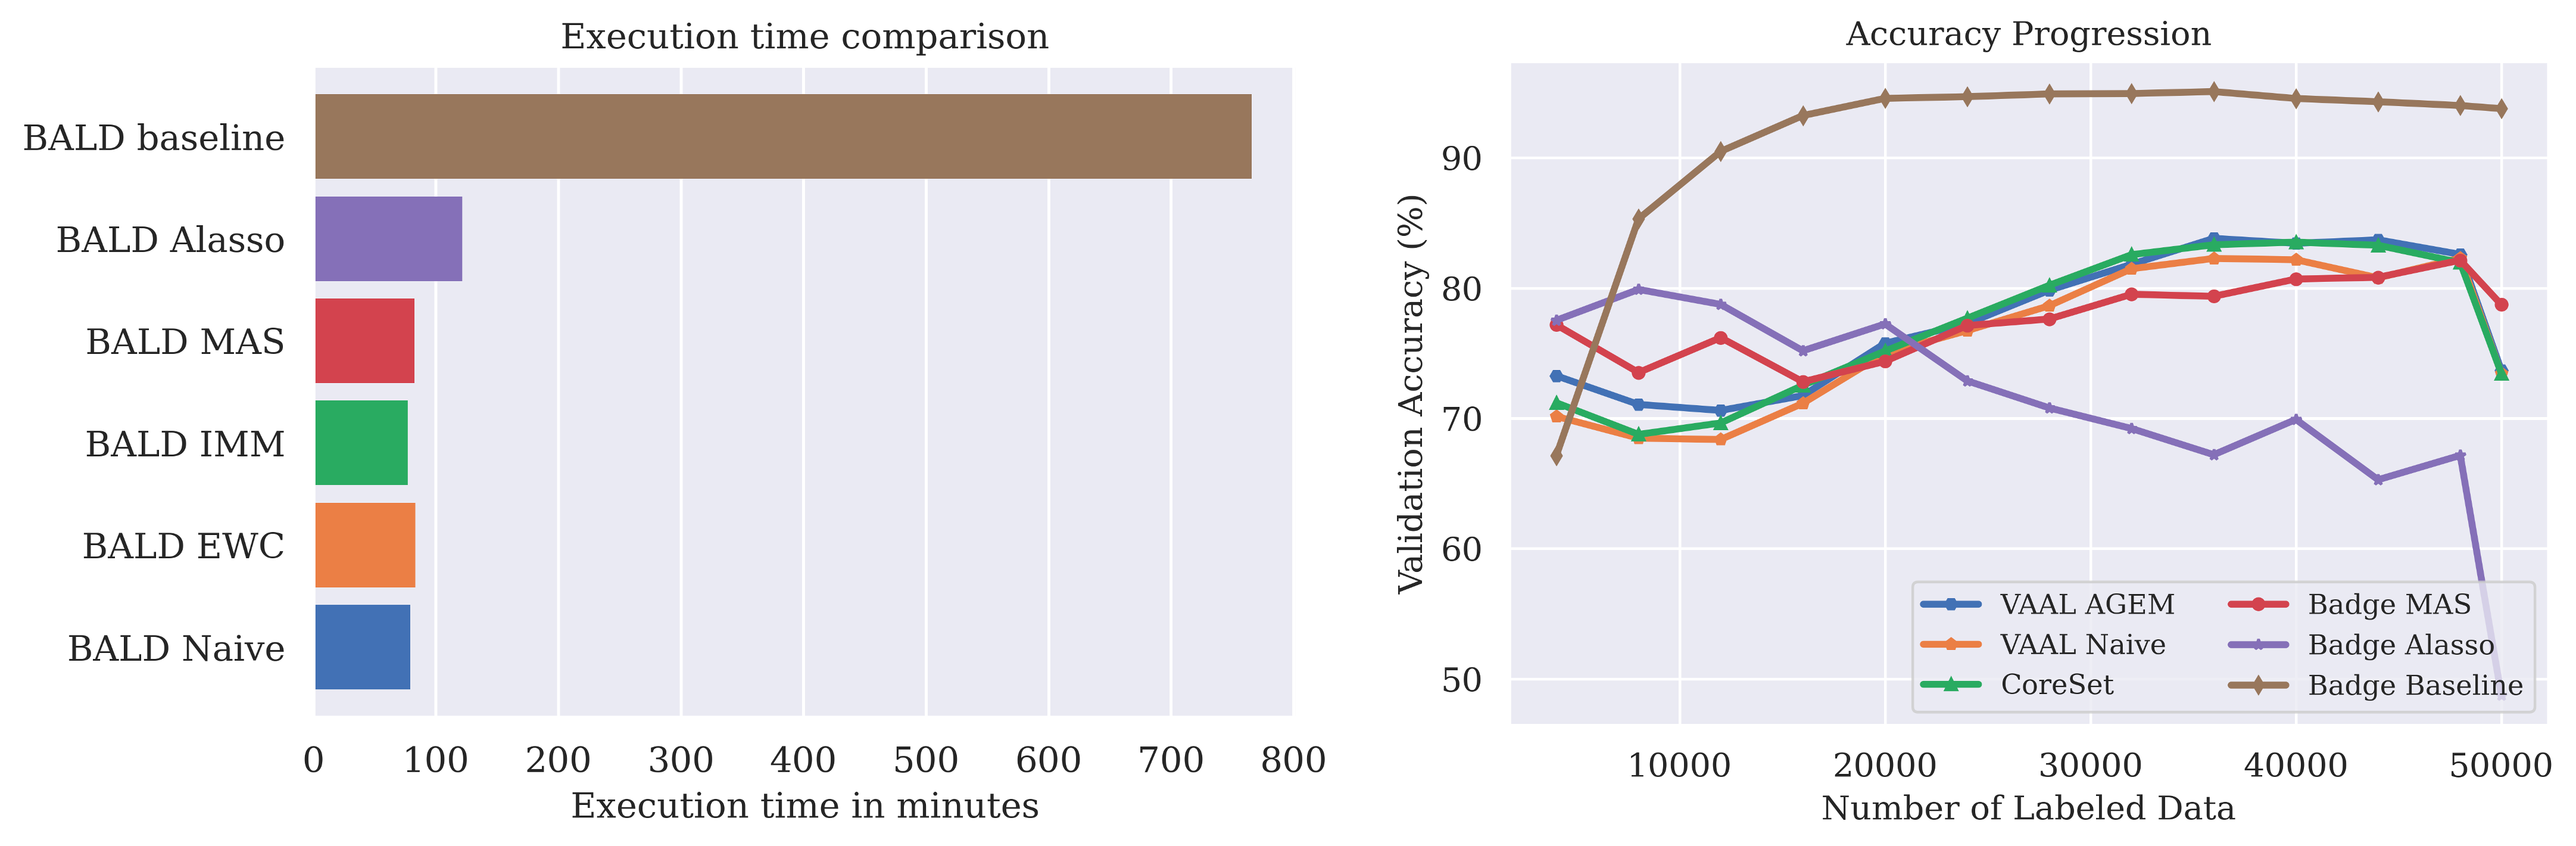
\includegraphics[width=\linewidth]{images/results_CAL/Bald_CAL_4000b.png}
    \caption[Continual Active Learning \gls{bald} 4000 batch size]{Comparison of execution time and validation accuracy of Continual Learning strategies used with the Active Learning strategy
    \gls{bald}. We use a batch size of 4000 for the experiments }
    \label{fig:Evaluation:Results:CAL:BALD4000}
\end{figure}


We now run the experiment with the identical setup with the Active Learning strategy CoreSet. Our results are presented in figure \ref{fig:Evaluation:Results:CAL:CoreSet4000}. The gap in execution time between the baseline and the Continual Learning 
strategies has further decreased. \gls{imm} is the fastest Continual Learning strategy, being about 6 times as fast as the baseline. On the other hand, \gls{alasso} is the slowest Continual Learning strategy, boasting around one fourth of the execution time of the
baseline. Not only the gap in execution time has decreased compared to the experiment with batch size 2000, but also the gap in validation accuracy. Naive is the best performing strategy, lacking only 10 percentage points in validation accuracy to the
baseline during the first half of the experiment. \gls{imm}, \gls{ewc} and \gls{mas} follow in that order, showing a similar validation accuracy curve as Naive. \gls{alasso} starts with a similar validation accuracy as the other Continual Learning strategies, but falls behind
after 8000 samples. \par


\begin{figure}[h]
    \centering
    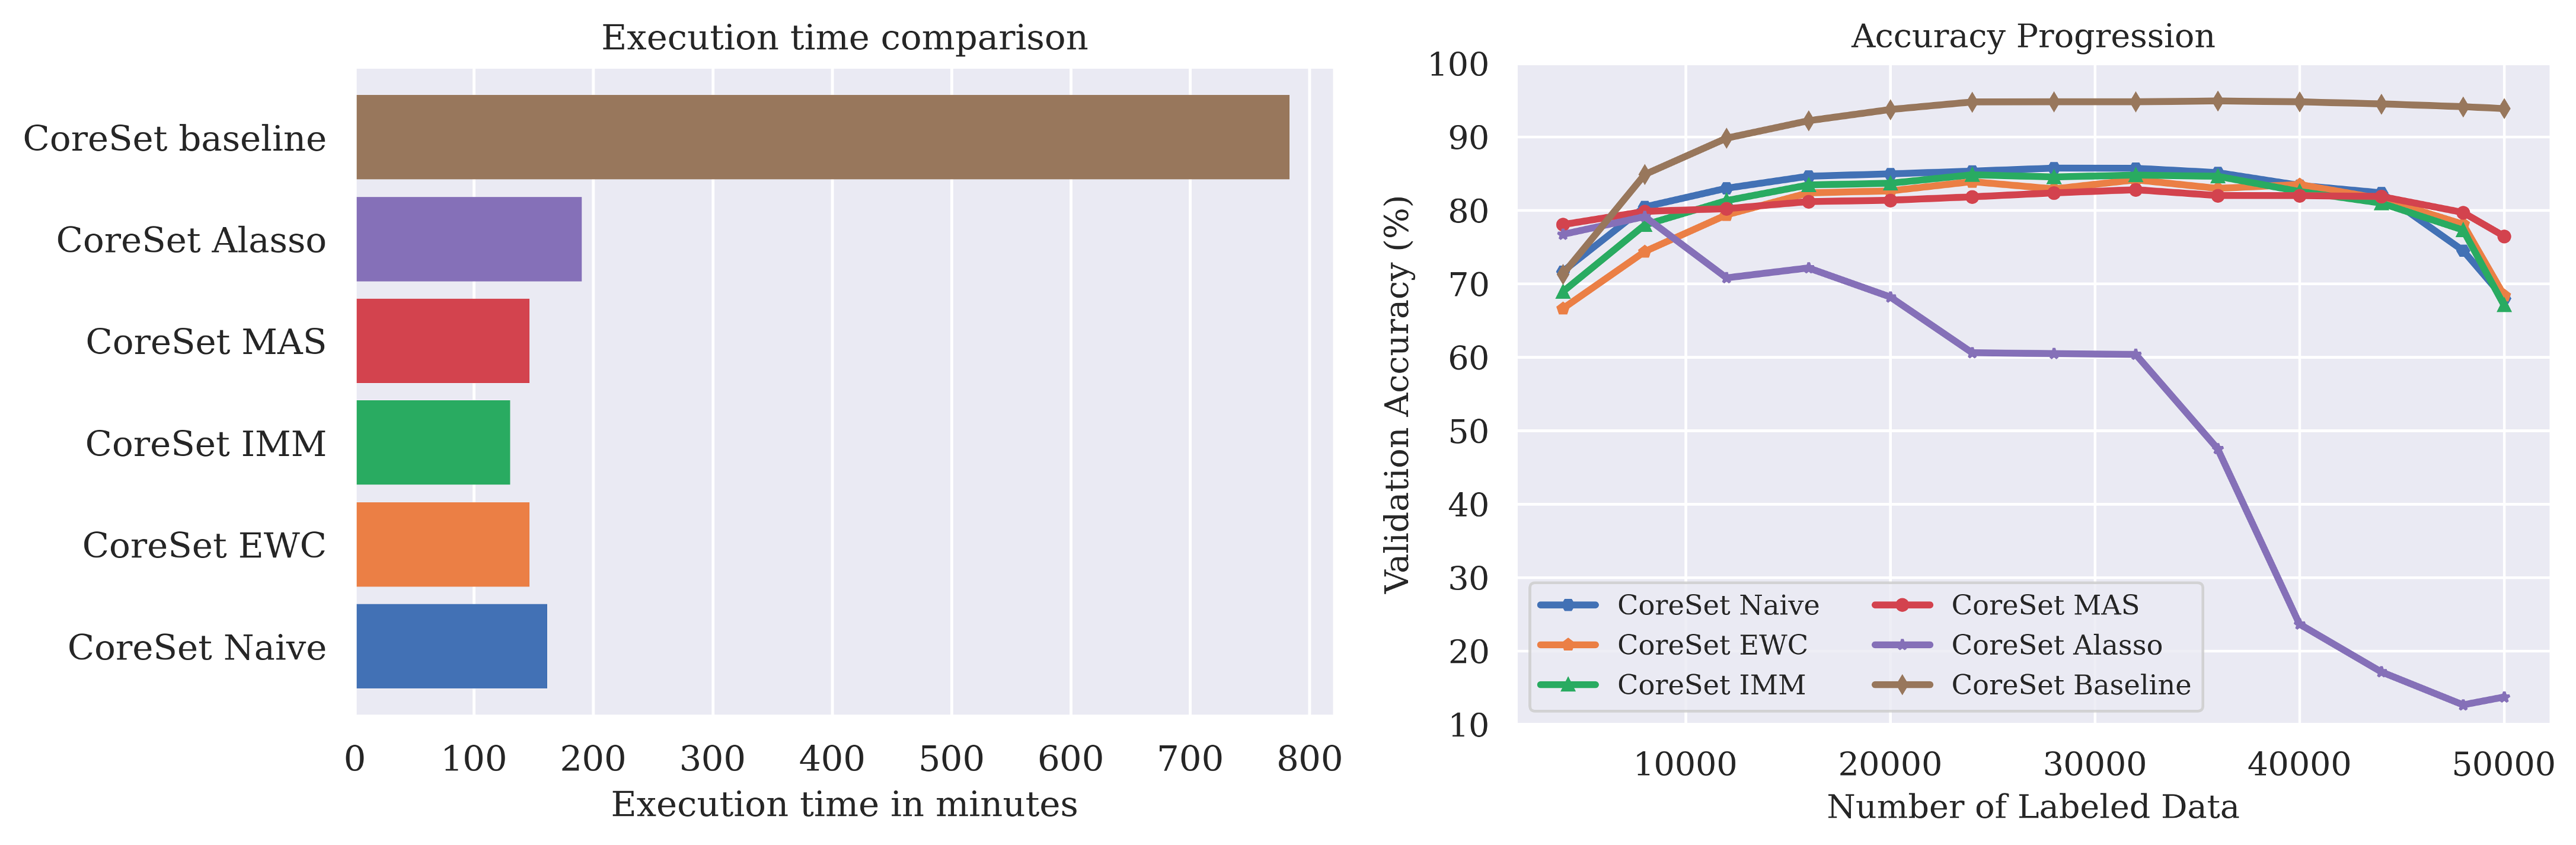
\includegraphics[width=\linewidth]{images/results_CAL/CoreSet_CAL_4000b.png}
    \caption[Continual Active Learning CoreSet 4000 batch size]{Comparison of execution time and validation accuracy of Continual Learning strategies used with the Active Learning strategy
    CoreSet. We use a batch size of 4000 for the experiments.}
    \label{fig:Evaluation:Results:CAL:CoreSet4000}
\end{figure}

Our final experiment with a batch size of 4000 is run with the Active Learning strategy \gls{badge}. The results of the experiment can be found in figure \ref{fig:Evaluation:Results:CAL:Badge4000}. Out of all experiments in this series, this one shows the
smallest gap in execution time between the baseline and the Continual Learning strategies. However, the baseline is still about 800 Minutes or 13 hours slower than all Continual Learning strategies. Just as in the experiment with 2000 batch size, the
execution time of the Contiual Learning strategies is comparable, with \gls{alasso} being the slowest and \gls{imm} being the fastest. Compared to the experiment with batch size 2000, the validation accuracy curve of all Continual Learning strategies has become smoother 
and the gap between the baseline and the Continual Learning strategies has decreased. The only exception to this is \gls{alasso}, which has a negative slope in its validation accuracy curve in the first half of the experiment, followed by a slight increase in 
validation accuracy and a huge drop in the end. \gls{imm}, \gls{ewc} and Naive perform similar for the first 45000 samples, where \gls{imm} falls behind the other two strategies. The validation accuracy of \gls{mas} is almost consistent throughout the experiment, with a slight
increase in the first half and a slight decrease in the second half. \par

\begin{figure}[h]
    \centering
    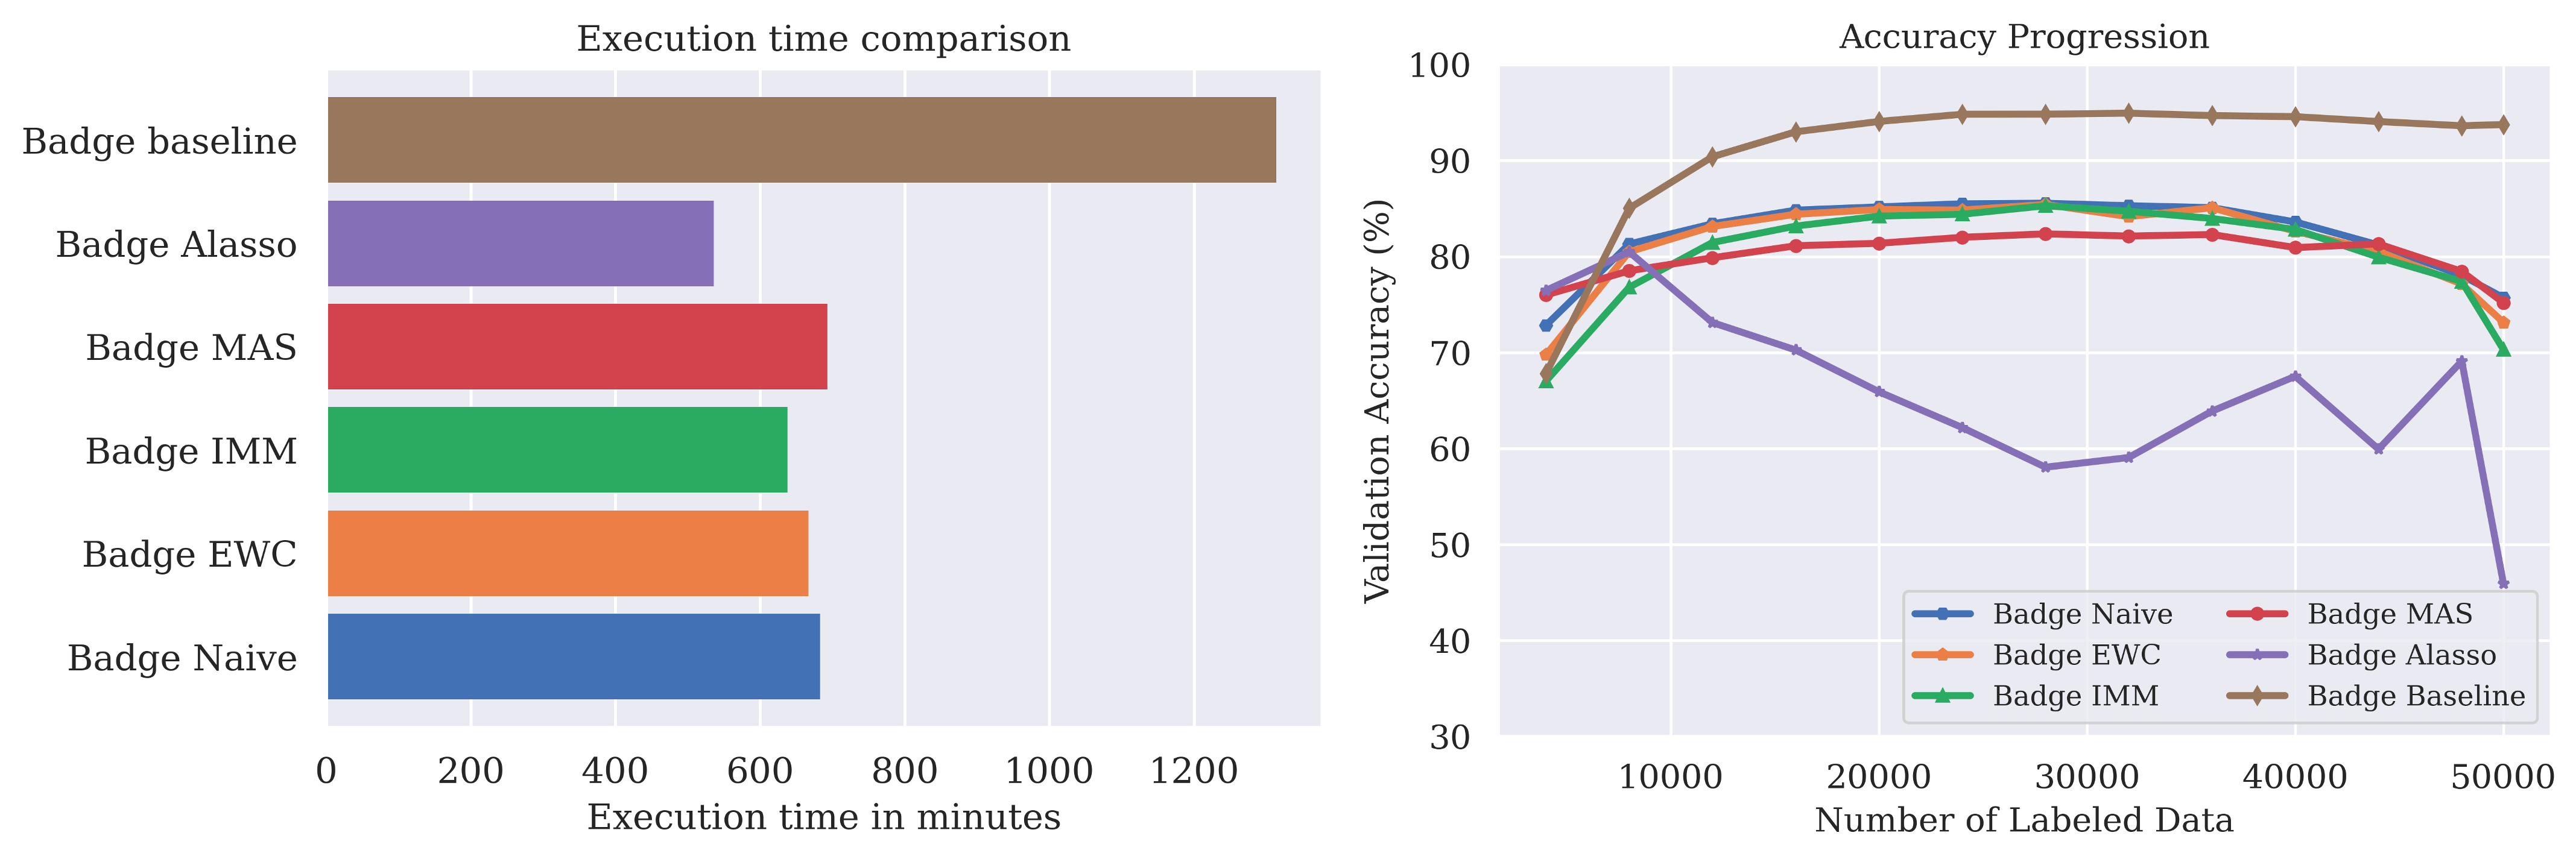
\includegraphics[width=\linewidth]{images/results_CAL/Badge_CAL_4000b.png}
    \caption[Continual Active Learning \gls{badge} 4000 batch size]{Comparison of execution time and validation accuracy of Continual Learning strategies used with the Active Learning strategy
    \gls{badge}. We use a batch size of 4000 for the experiments.}
    \label{fig:Evaluation:Results:CAL:Badge4000}
\end{figure}

\subsubsection{A hybrid approach to Continual Learning}
\label{sec:Evaluation:Results:CAL:Hybrid}
After running the experiments in section \ref{sec:Evaluation:Results:CAL:ALCL}, we notice that all of them demonstrate a significant discrepancy in validation accuracy between Active Learning and Continual Active Learning. To further investigate this gap,
we investigate a hybrid approach where we run Active learning for the first $i$ iterations before switching to Continual Active Learning. With these experiments we hope to decrease the gap in validation accuracy to Active Learning. We vary $i$ between 0 and 6,
and perform two sets of experiments, one using the Continual Learning strategy \gls{mas} and the other using \gls{ewc}. In both experiments, we use the Active Learning strategy \gls{badge}. The results of the two sets of experiments can be found in figure 
\ref{fig:Evaluation:Results:CAL:DelayedStart}. For \gls{mas} and \gls{ewc}, the validation accuracy drops immediately after switching from Active Learning to Continual Active Learning. However, in the long run the \gls{mas} strategy retains the validation accuracy better than \gls{ewc}.
We also notice that while the validation accuracy does drop after switching to Continual Active Learning, it is higher at a fixed cycle than when switching to Continual Active Learning in an earlier cycle. \par

\begin{figure}[h]
    \centering
    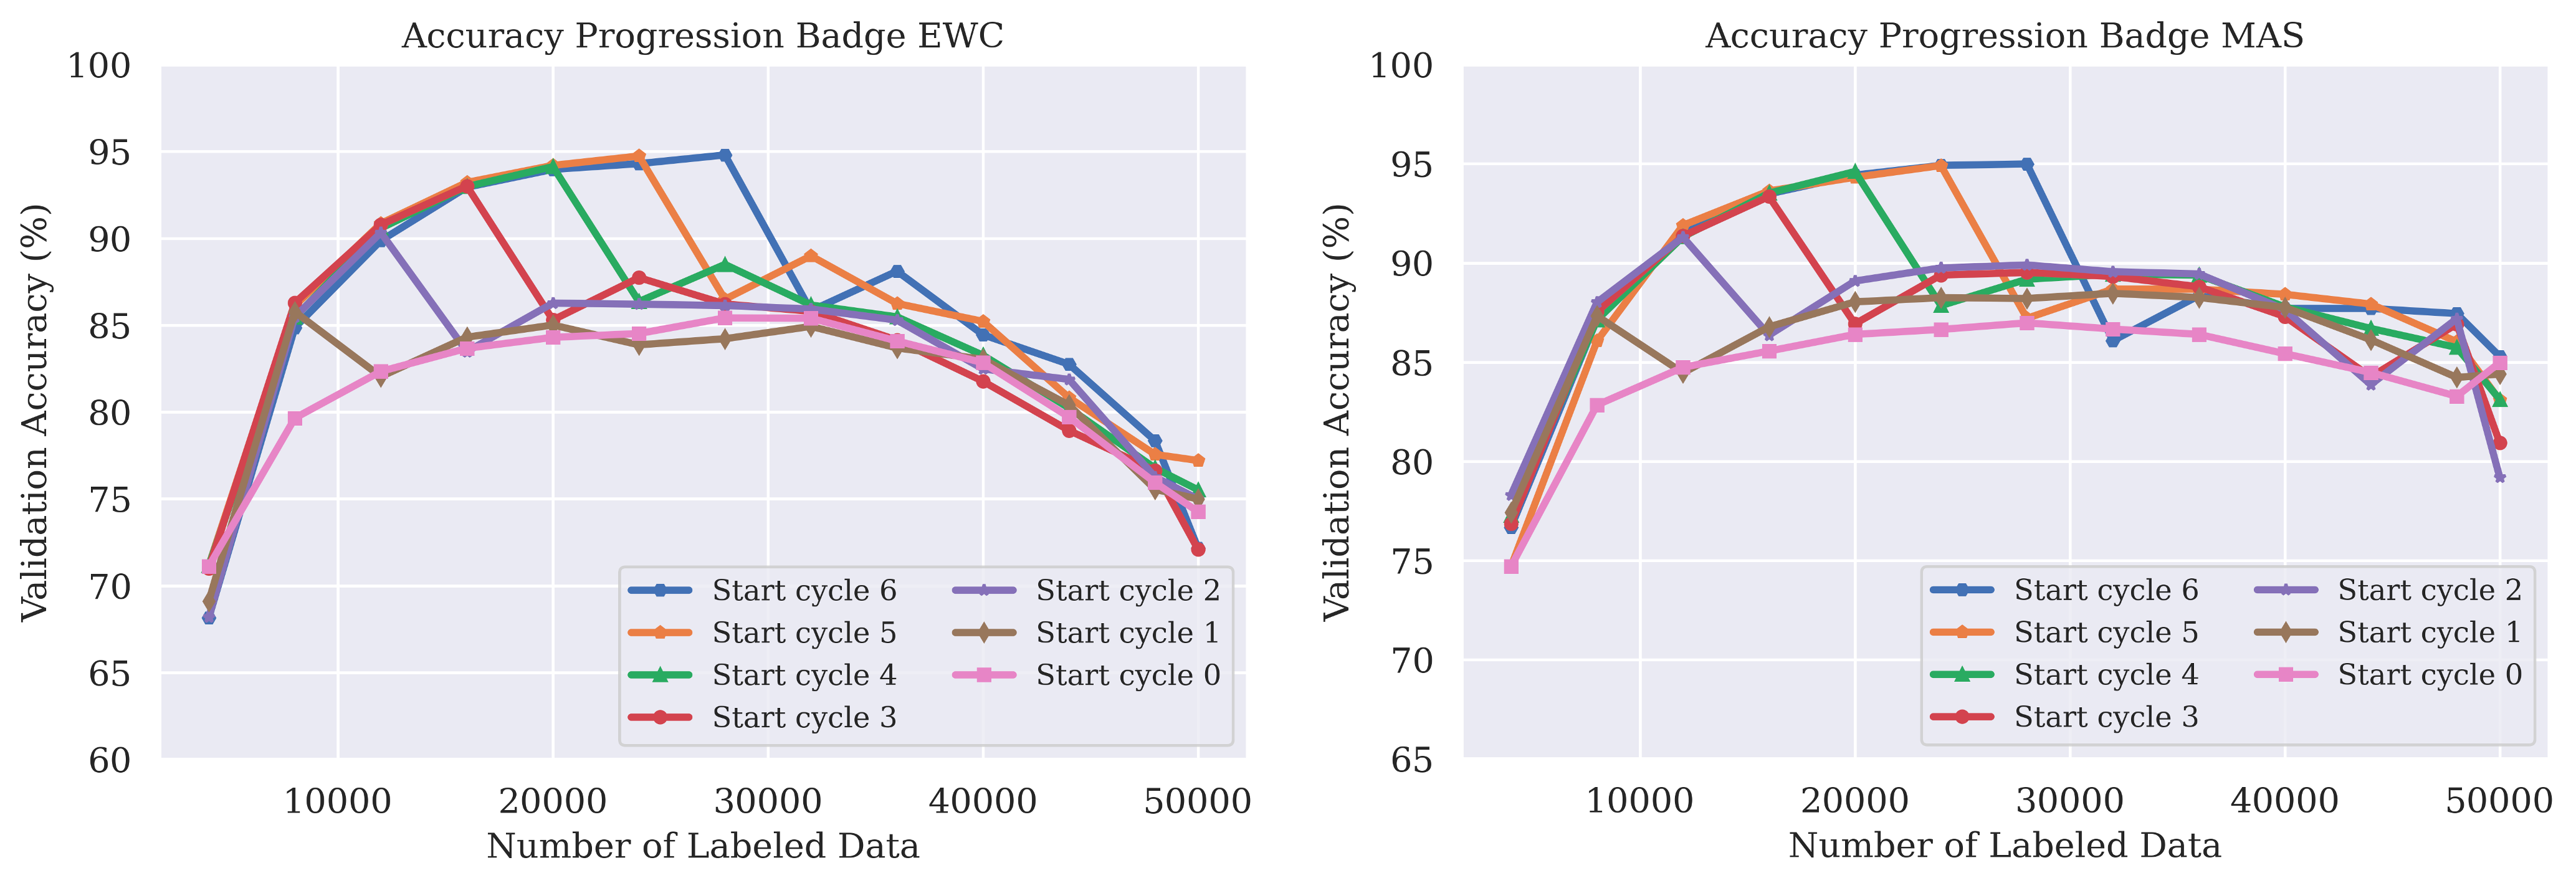
\includegraphics[width=\linewidth]{images/results_CAL/Delayed_start_CAL.png}
    \caption[Continual Active Learning Hybrid approach]{Comparison of validation accuracy for a delayed start of Continual Learning. Left: Accuracy progression for \gls{badge} and \gls{ewc}. Right: Accuracy progression for \gls{badge} and \gls{mas}.}
    \label{fig:Evaluation:Results:CAL:DelayedStart}
\end{figure}

\subsubsection{Varying the initialization of the labeled pool}
\label{sec:Evaluation:Results:CAL:Initialization}
Motivated by the findings from the previous section, we wonder if the initialization of the labeled pool has an impact on the validation accuracy of the Continual Learning strategies. Beck et al.\cite{beck2021effective} show that using a facility location selection 
\cite{iyer2021submodular} yields better validation accuracy when training on the initial labeled pool. We therefore test the effect of an initialization using the facility location selection compared to our random initialization. As our Active Learning strategy,
we use \gls{badge} with a batch size of 4000 and \gls{mas} as our Continual Learning strategy. The results of the experiment can be found in figure \ref{fig:Evaluation:Results:CAL:FLinit}. While the facility location approach performs better than random initialization, the difference is
marginal. Interestingly, the validation accuracy of the facility location approach is lower than the random initialization in the first iteration. The most significant drawback of the facility location initialization is its resource-intensity. Initialization with facility
location takes about 24 hours to complete and requires more than 100GB of memory for CIFAR-10 using the implementation proposed by Beck et al. \cite{beck2021effective}. \par

\begin{figure}[h]
    \centering
    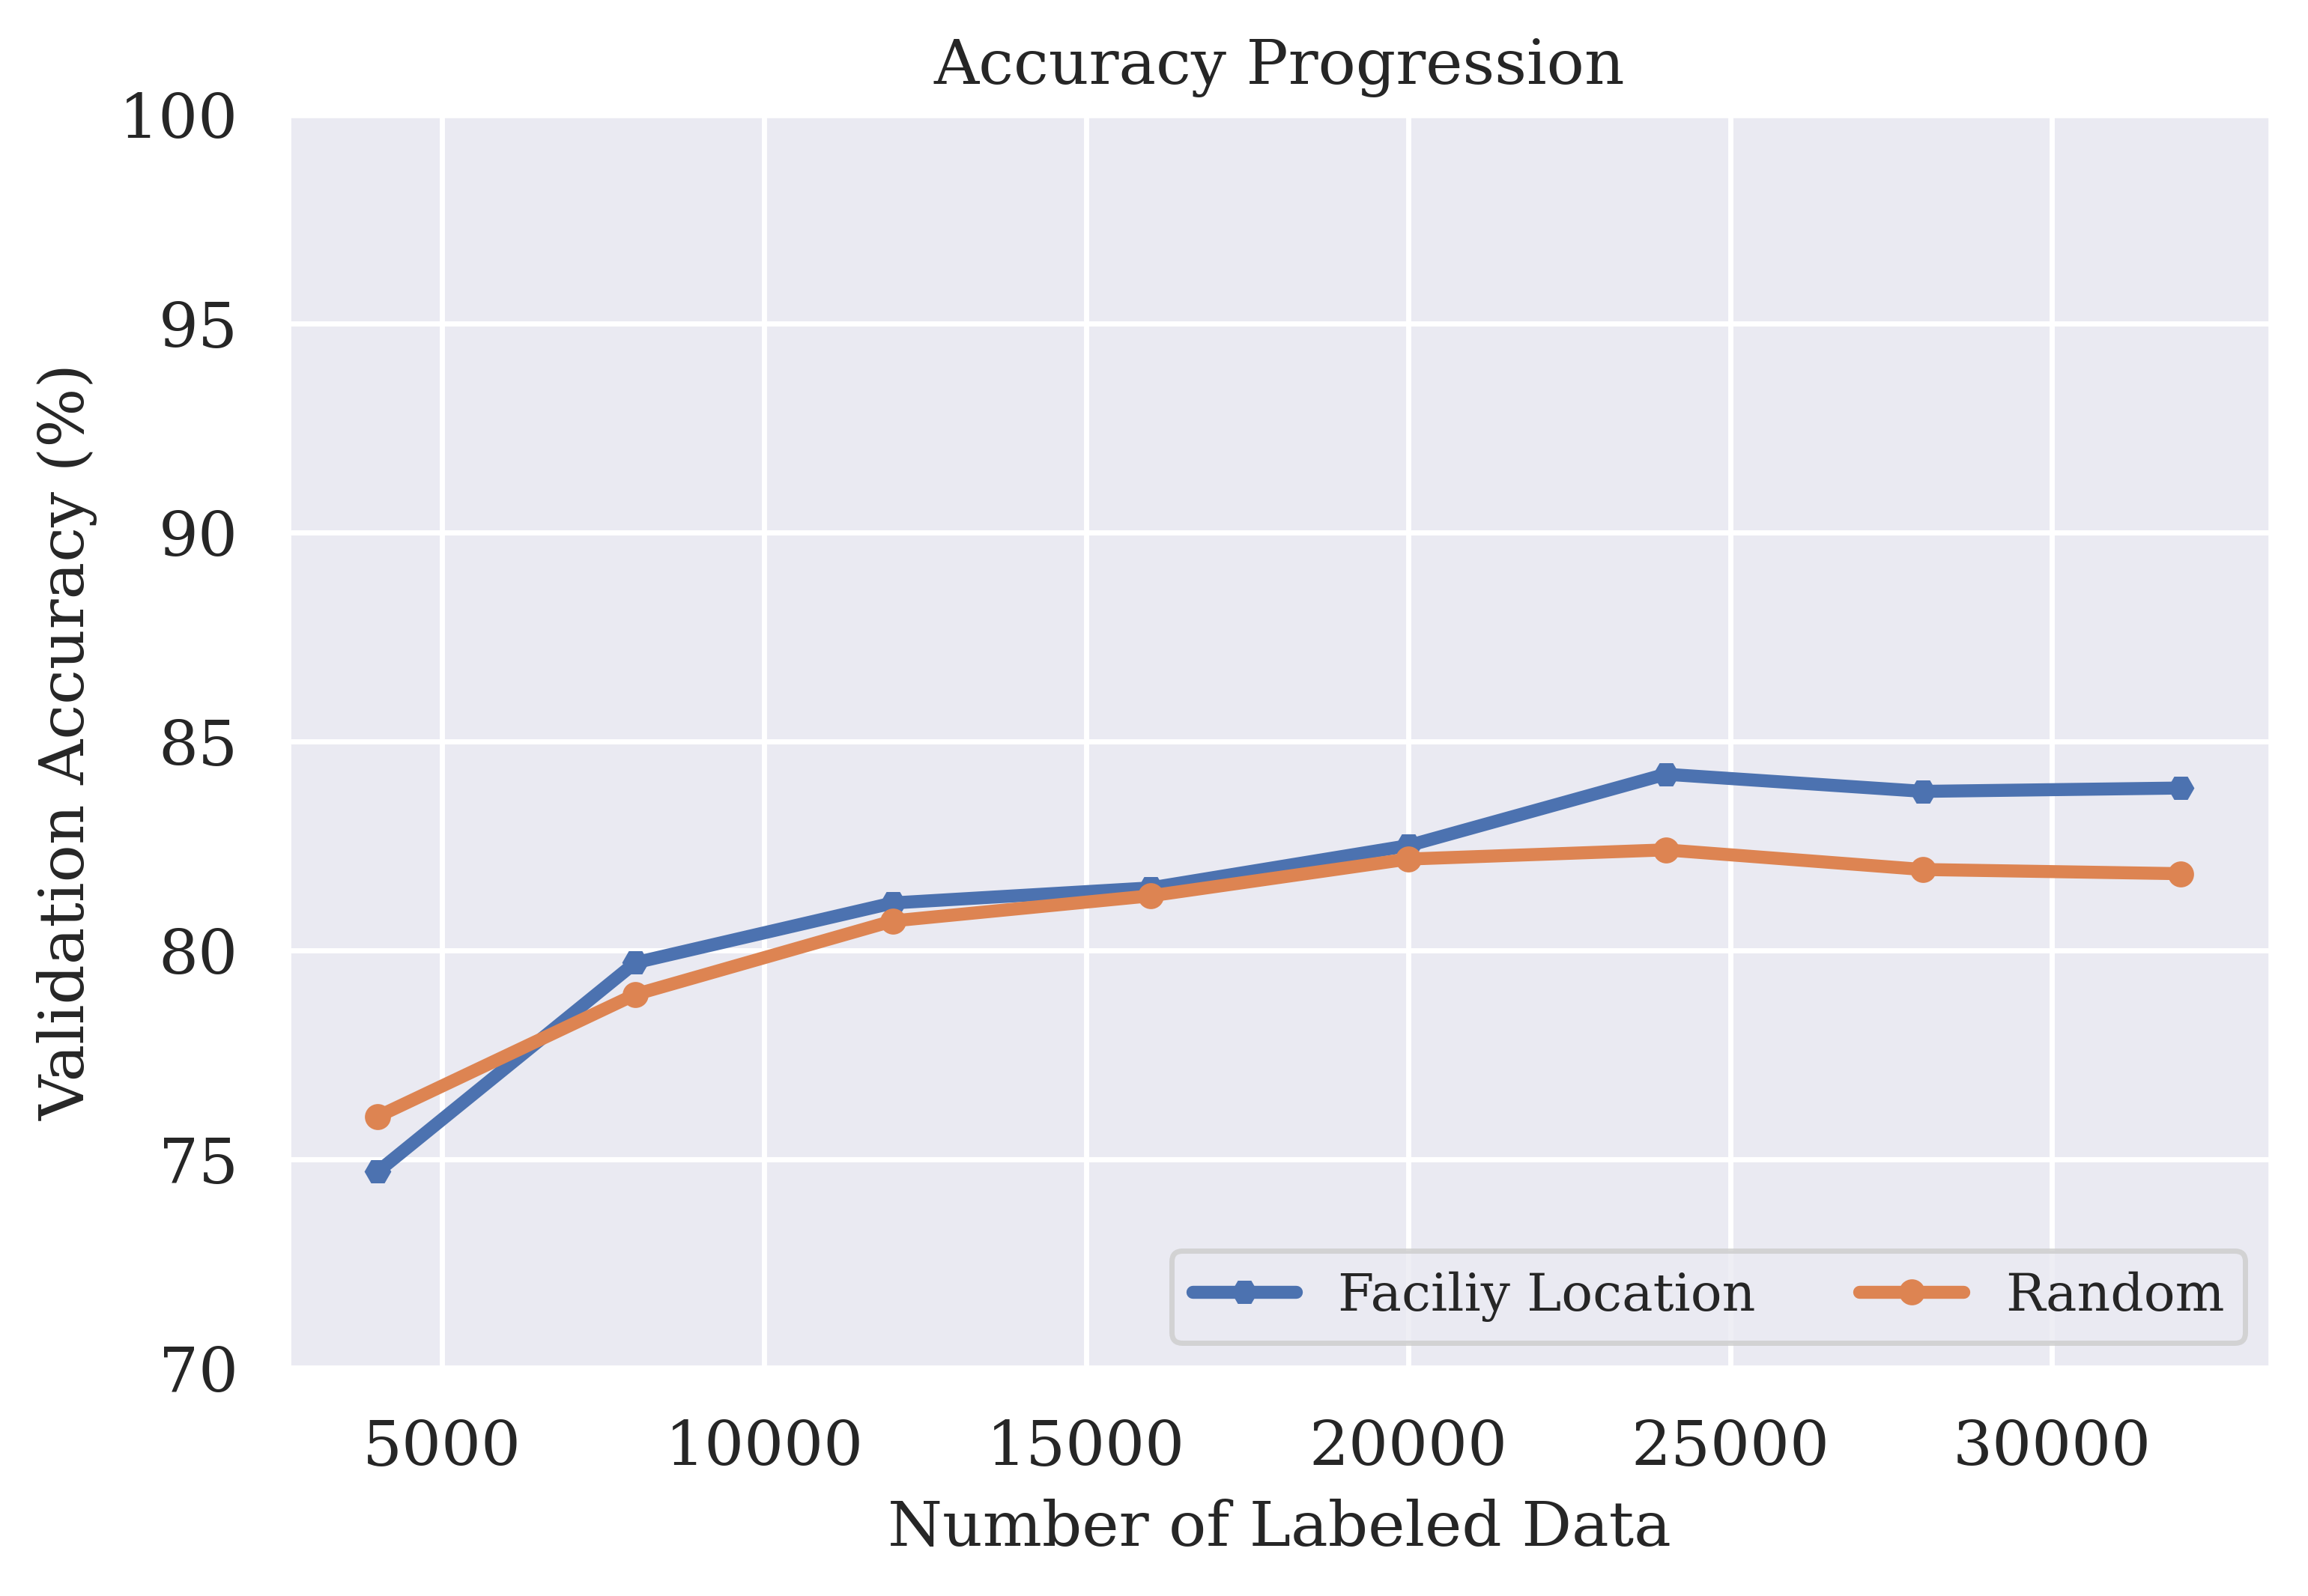
\includegraphics[width=\linewidth]{images/results_CAL/Facility_location_init.png}
    \caption[Initialization using Facility Location]{Comparison of validation accuracy for facility location initialization and random initialization. We use a batch size of 4000 and the combination of \gls{badge} and \gls{mas} for the experiments.}
    \label{fig:Evaluation:Results:CAL:FLinit}
\end{figure}


\subsubsection{Custom Replay approach}
\label{sec:Evaluation:Results:CAL:Replay}
In section \ref{sec:Methodology:ReplayStrategy} we propose a custom replay strategy for Continual Active Learning. The use of our replay strategy is motivated by the main finding of section \ref{sec:Evaluation:Results:CAL:ALCL}: the validation accuracy increases with an
increased batch size. In this set of experiments, we use the Active Learning strategy CoreSet and vary the batch size and the size of the replay buffer. Moreover, we investigate the effect of CoreSet selection in the replay buffer compared to random selection. We present our
results in figure \ref{fig:Evaluation:Results:CAL:Replay}. When varying the batch size and buffer size, we notice that increasing the buffer size and the batch size yields a higher validation accuracy. However, our replay strategy does not outperform the Naive approach when using
the same amount of training data (i.e. batch size + replay buffer size for the replay strategy and batch size for the Naive approach). To evaluate the importance of CoreSet selection in the buffer compression process, we compare the validation accuracy of our replay strategy
when using CoreSet selection and random selection. We notice that the validation accuracy remains largely the same for both buffer compression methods, apart from the last 15000 samples, where CoreSet selection outperforms random selection. \par

\begin{figure}[h]
    \centering
    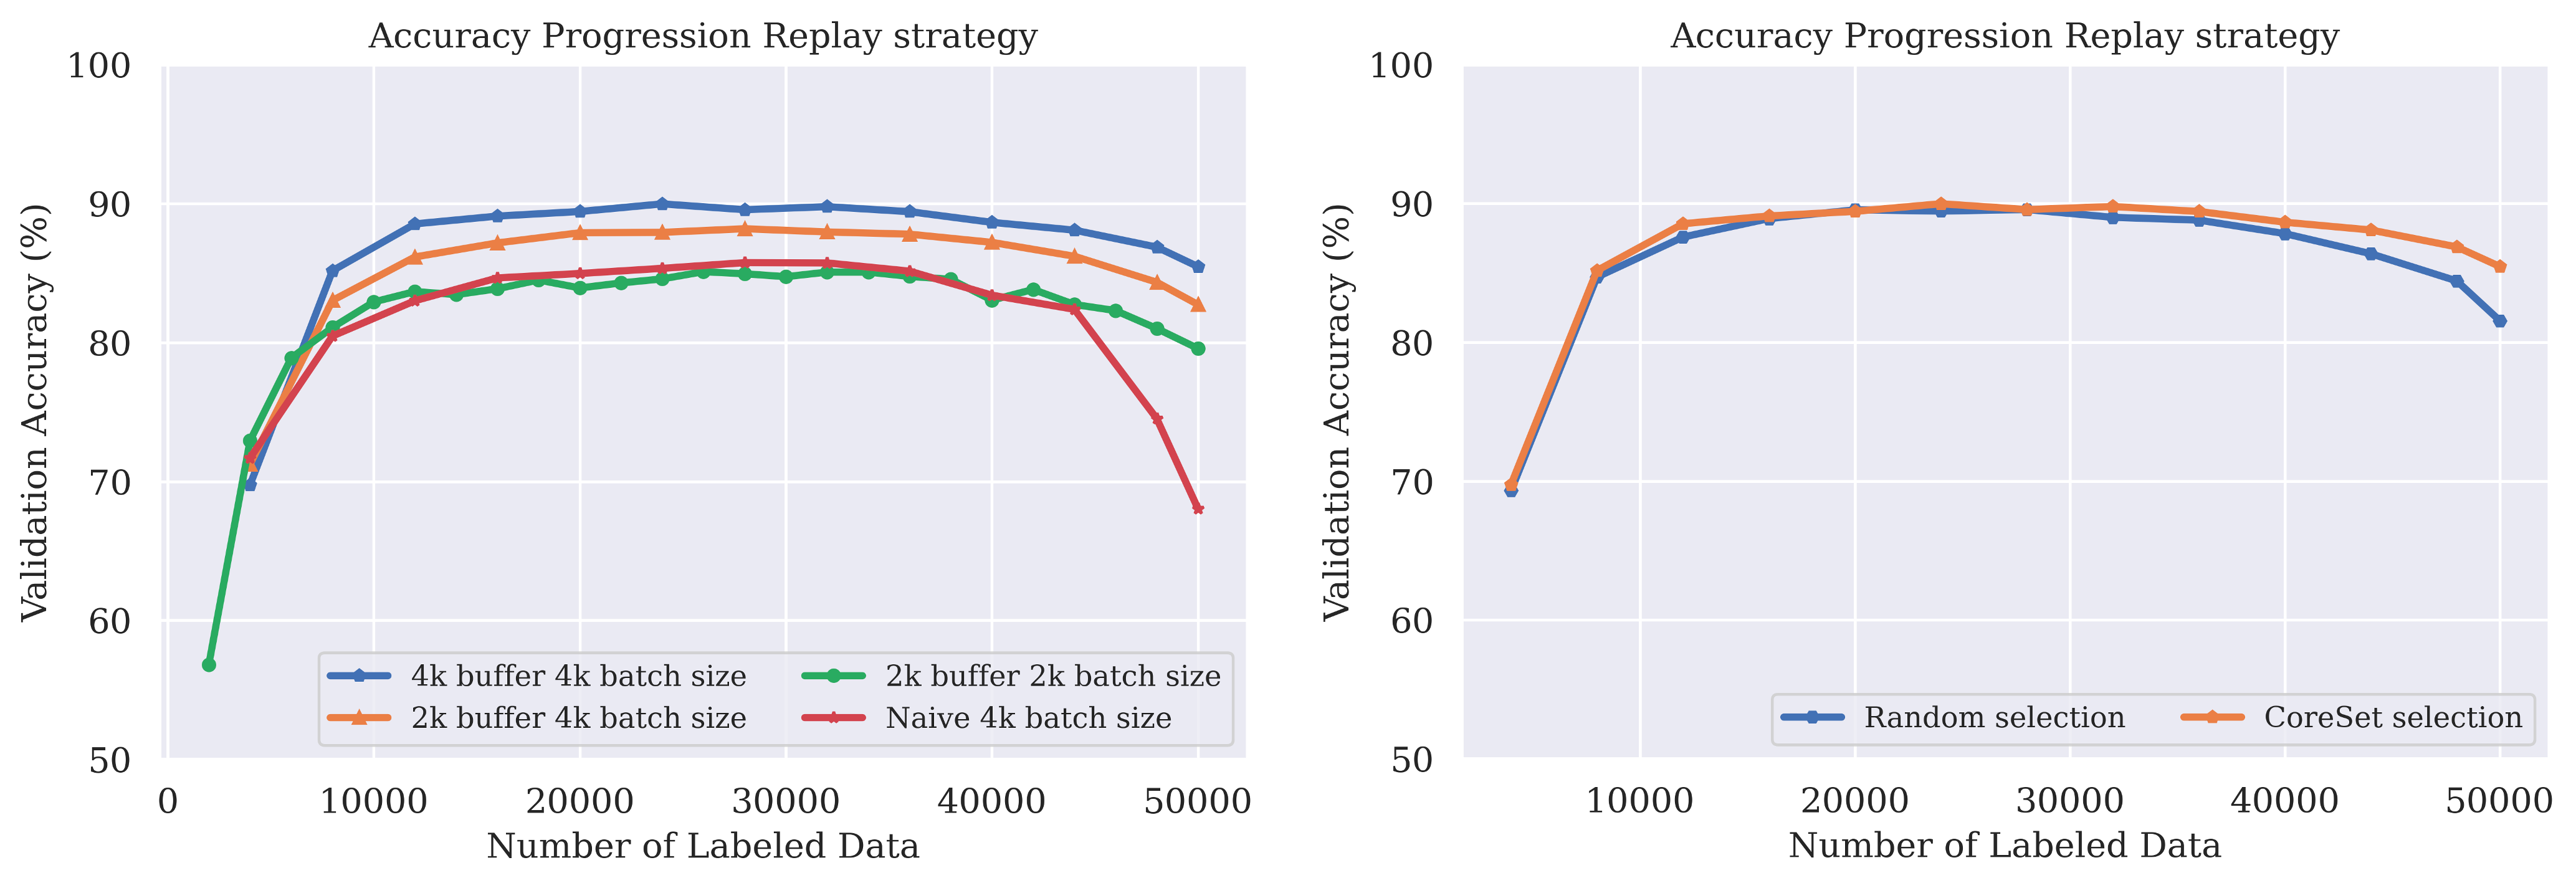
\includegraphics[width=\linewidth]{images/results_CAL/replay_CAL.png}
    \caption[Continual Active Learning Custom Replay strategy]{Left: Comparison of validation accuracy of our Replay strategy with different hyperparameters. Right: Comparison of validation accuracy of our Replay strategy when using different buffer compression approaches.
    In both runs, we use a batch size of 4000 and a replay buffer size of 4000.}
    \label{fig:Evaluation:Results:CAL:Replay}
\end{figure}

\subsubsection{VAAL and \gls{a-gem}}
\label{sec:Evaluation:Results:CAL:VAAL_AGEM}
Unsatisfied with the results from previous experiments, we decide to implement further Continual and Active Learning strategies. We perform an extensive literature search, investigating the suitability of representation-based Active Learning strategies and Continual Learning
strategies from the Exemplar Rehearsal category in the summary paper by Mundt et al. \cite{mundt2020wholistic}. The Active Learning strategy which we implement is \gls{vaal} \cite{sinha2019variational} and the Continual Learning strategy is \gls{a-gem} \cite{chaudhry2019continual}. We decide
to implement \gls{vaal} because it is the only representation-based Active Learning strategy which consistently performs better than random sampling. The reason why we choose to implement \gls{a-gem} as our Continual Learning strategy is that is one of the few Exemplar Rehearsal strategies
applicable to (Semi-) supervised Learning (many other strategies focus on Reinforcement Learning) while being computationally efficient and demonstrating strong performance in the experiments by Chaudhry et al. \cite{chaudhry2019continual} at the same time. \par
First, we analyze the performance of \gls{vaal} as an Active Learning strategy. We run \gls{vaal} with a batch size of 4000 and compare it to Random and CoreSet. We choose Random because it is the baseline for Active Learning strategies and CoreSet because it is among the best performing Active
we used before. The results can be found in the left plot in figure \ref{fig:Evaluation:Results:CAL:VAAL}. While \gls{vaal} outperforms random sampling by a large margin, it is itself outperformed by about the same margin by Coreset. To ensure that the results are not due to a
suboptimal hyperparameter choice, we run \gls{vaal} training VAE and Discriminator for 20 epochs in one run and 100 epochs in another. Because we are interested in the performance of \gls{vaal} in our Continual Active Learning setting, we use Continual Active Learning with a batch size of 4000
and the Continual Learning strategy Naive. We present the results of the experiment in the right plot of figure \ref{fig:Evaluation:Results:CAL:VAAL}. Surprisingly, the validation accuracy is marginally impacted by the training time of Generator and VAE. If anything, the validation
accuracy is higher when training for 20 epochs. \par

\begin{figure}[h]
    \centering
    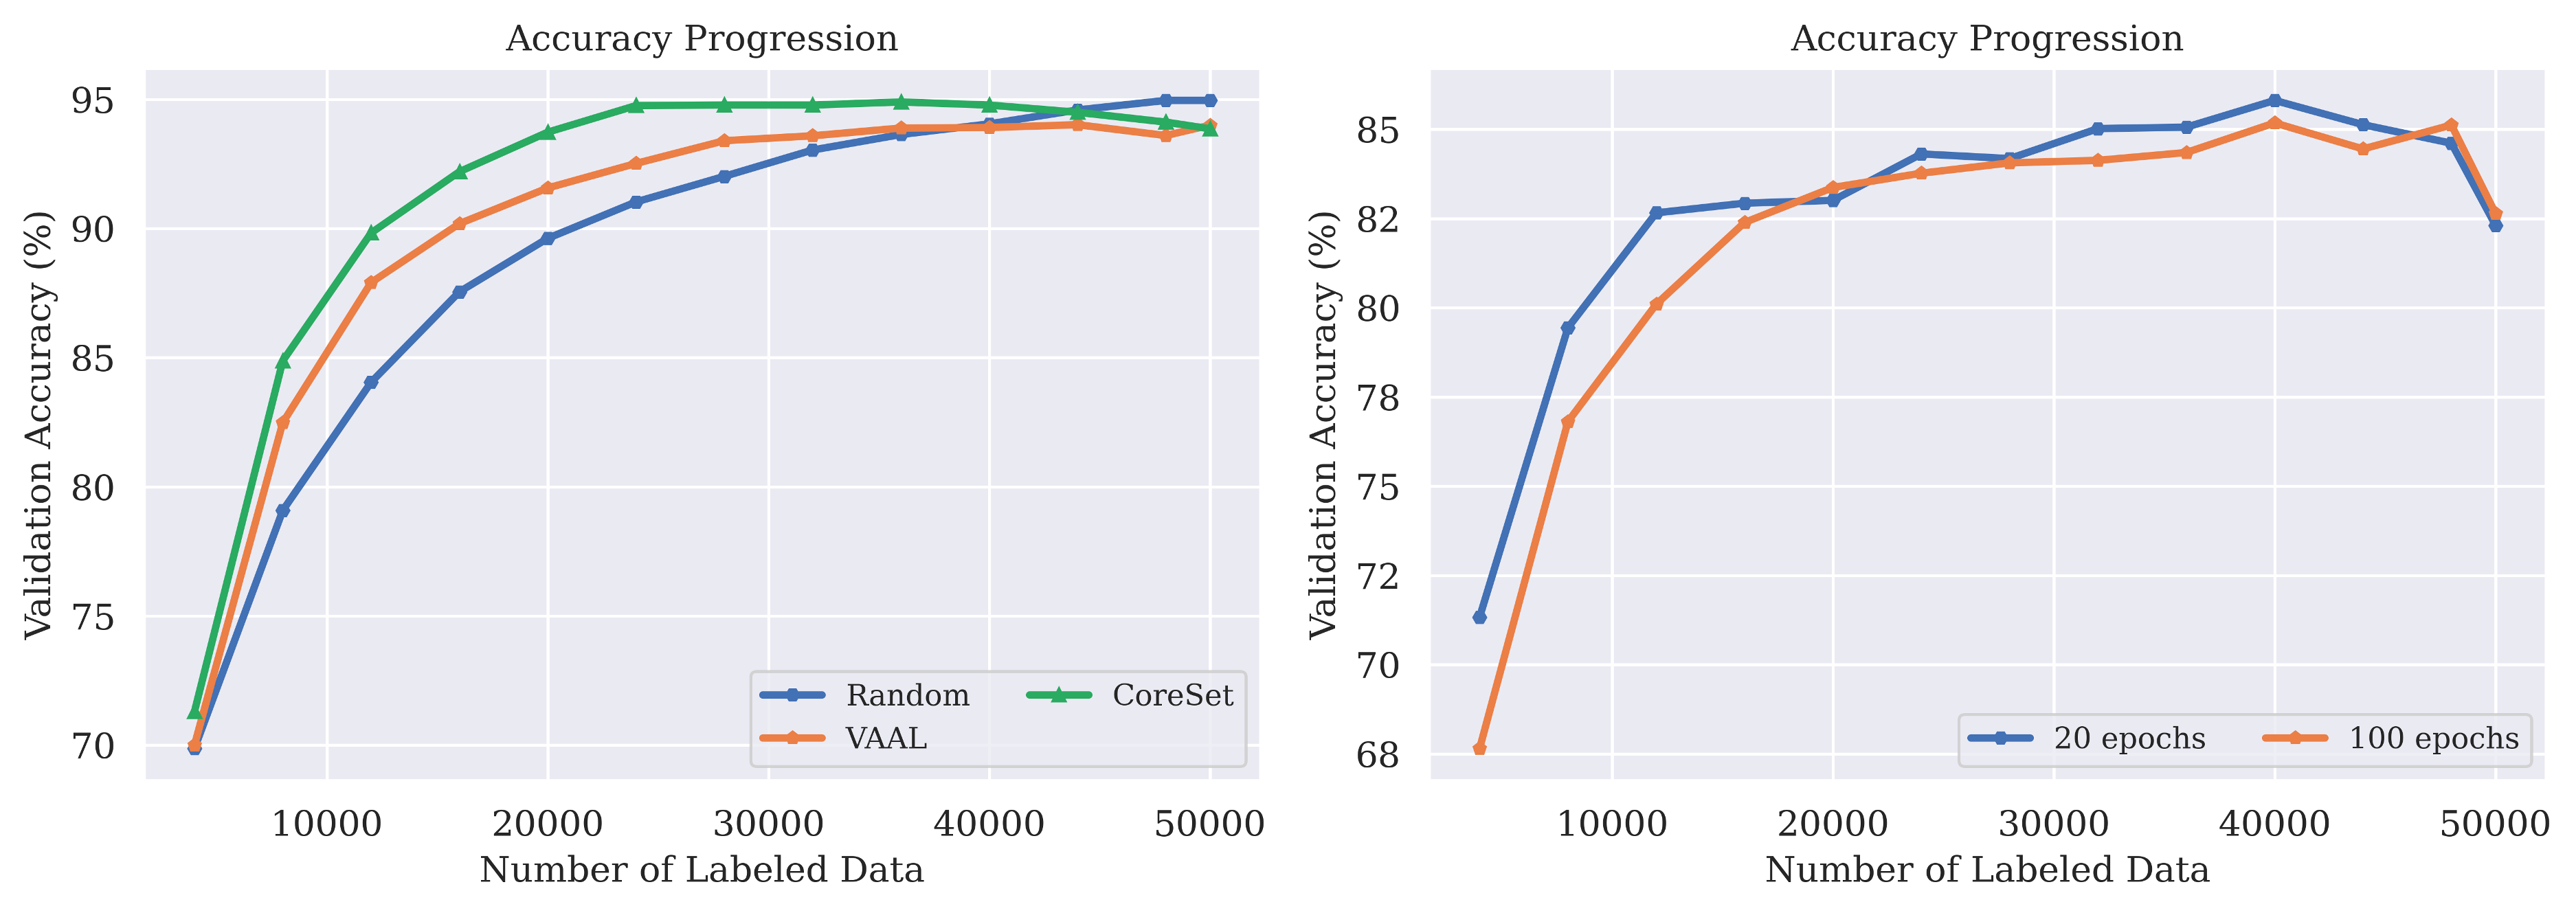
\includegraphics[width=\linewidth]{images/results_CAL/VAAL_plots.png}
    \caption[Continual Active Learning Custom Replay strategy]{Left: Comparison of validation accuracy of \gls{vaal} to the Active Learning strategies Random and CoreSet. We use a batch size of 4000 for the experiments. Right: Comparison of validation accuracy when varying the training 
    epochs for VAE and Discriminator. We use Continual Active Learning with the Naive approach as our Continual Learning strategy and a batch size of 4000.}
    \label{fig:Evaluation:Results:CAL:VAAL}
\end{figure}

Next, we experiment with \gls{a-gem}. \gls{a-gem} has two hyperparameters: $S$, which is the number of samples randomly drawn from the memory to compute the reference gradients and $P$ which is the number of data points stored to the memory from each task. We run \gls{a-gem} with the Active Learning
strategy \gls{lc} and a batch size of 2000. To assess the performance of \gls{a-gem}, we compare its validation accuracy to the Naive approach. We vary $S$ and $P$ and present our results in the right plot of figure \ref{fig:Evaluation:Results:CAL:AGEM}. The validation accuracy increases with
an increased $S$ and $P$ until about 12000 samples, after which the validation accuracy drops for all values of $S$ and $P$. \gls{a-gem} outperforms the Naive approach for the first 15000 samples, but is outperformed by Naive for the remainder of the experiment. \par
After investigating the influence of \gls{a-gem}'s hyperparameters, we compare the combination of \gls{vaal} and \gls{a-gem} to \gls{vaal} and Naive, using a batch size of 4000. The results are shown in the left plot of figure \ref{fig:Evaluation:Results:CAL:AGEM}. Although \gls{a-gem} performs worse than the Naive
approach when using the Active Learning strategy \gls{lc}, it outperforms the Naive approach when using \gls{vaal} as the Active Learning strategy. \par

%TODO: Redo right plots
\begin{figure}[h]
    \centering
    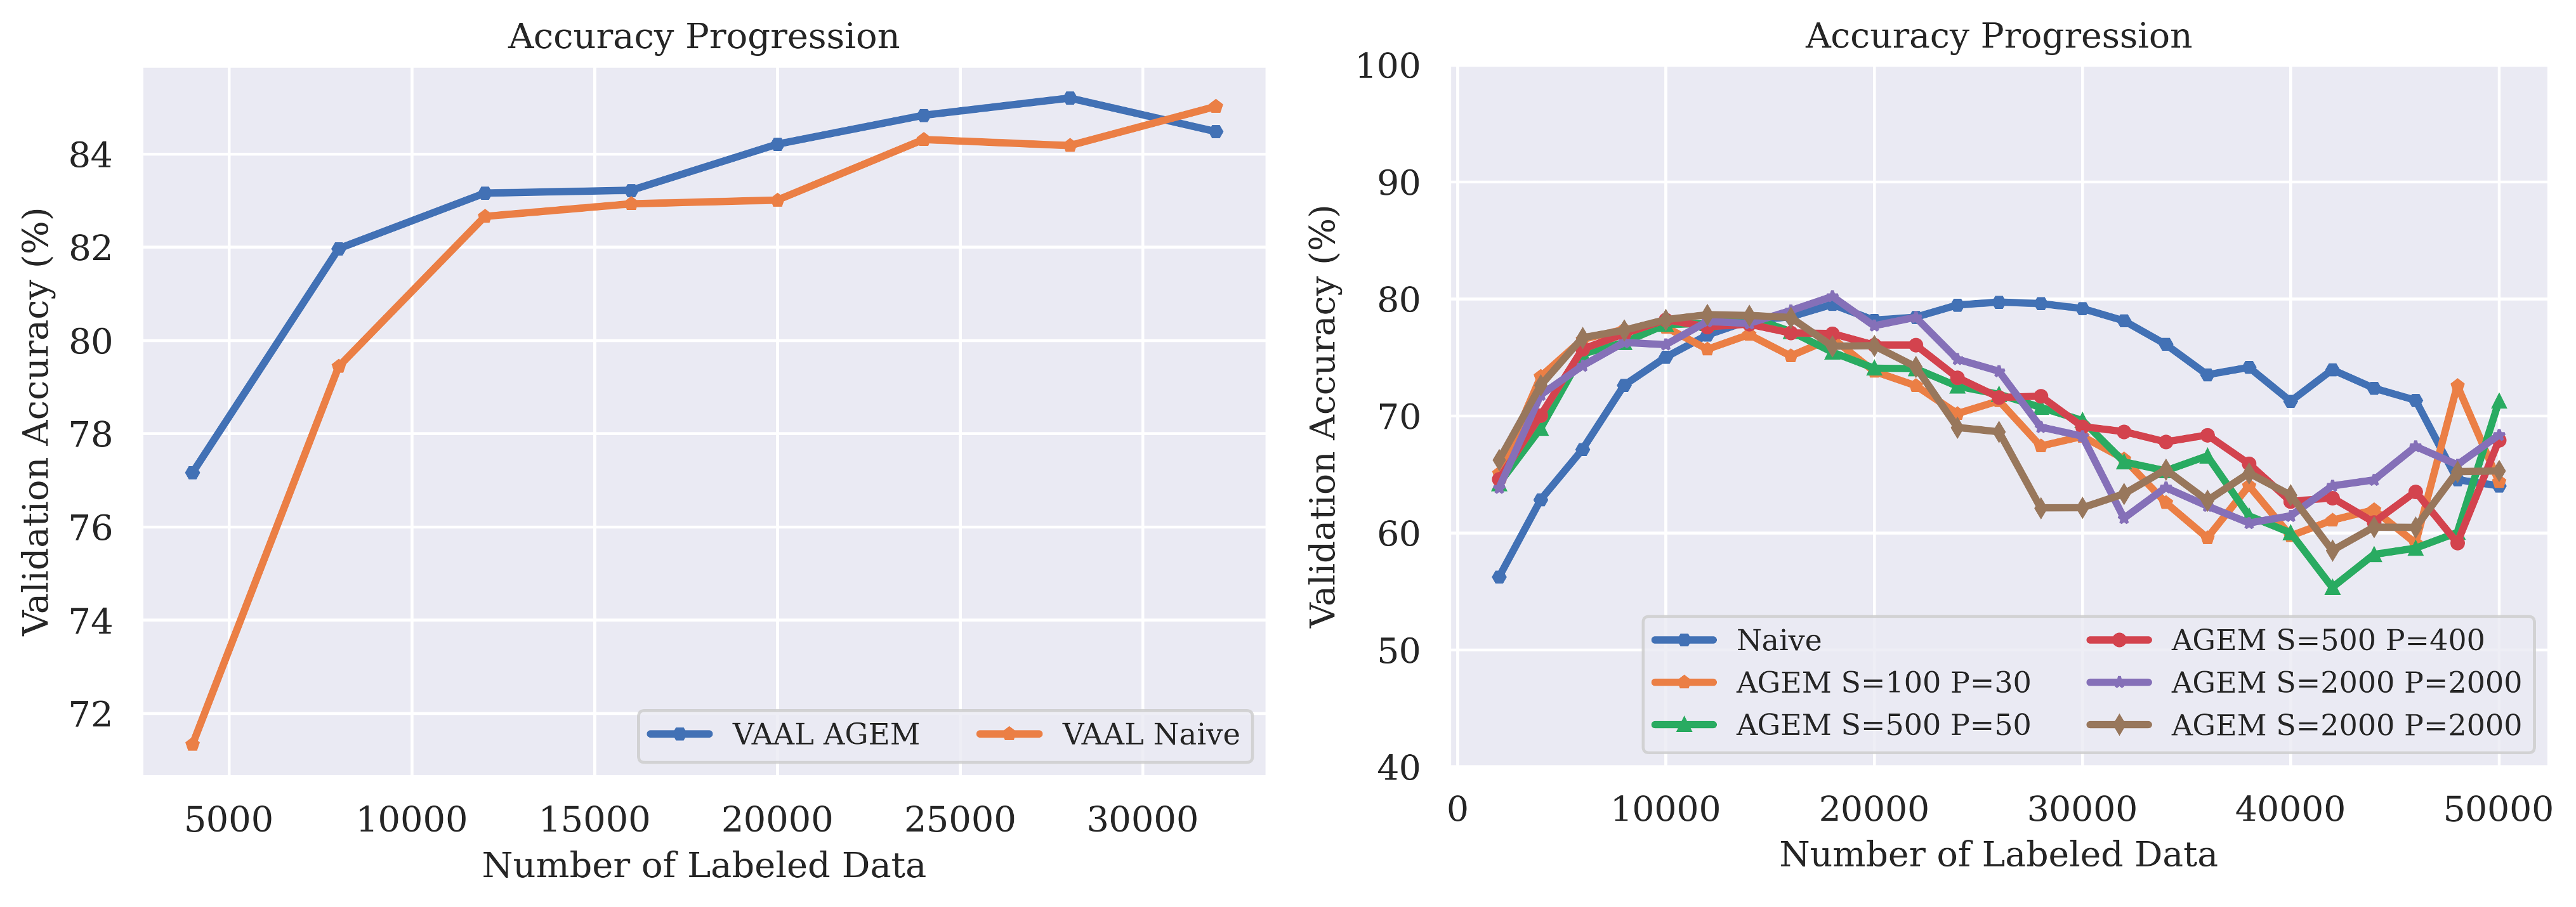
\includegraphics[width=\linewidth]{images/results_CAL/AGEM_plots.png}
    \caption[Continual Active Learning Custom Replay strategy]{Left: Comparison of validation accuracy of \gls{a-gem} to the Naive approach when using \gls{vaal} as the Active Learning strategy We use a batch size of 4000 for the experiments. Right: Comparison of validation accuracy of \gls{a-gem}
     to the Naive approach when using different values of $S$ and $P$. We use the Active Learning strategy \gls{lc} and a batch size of 2000 for the experiments.}
    \label{fig:Evaluation:Results:CAL:AGEM}
\end{figure}

\subsection{Model Stealing Results}
\label{sec:Evaluation:Results:MS}
After extensively studying Continual Active Learning, we shift the focus of our experiments to Model Stealing. Since we build our work on the ActiveThief framework, we first evaluate the performance of the ActiveThief framework, including the influence of Model Architecture and
Thief Dataset as well as the difference between stealing a target model returning the predicted labeled and stealing a target model returning the softmax outputs of the final model layer. After experimenting with the ActiveThief framework, we evaluate the performance of our pro
-posed Continual Active Learning strategy for Model Stealing attacks. We perform the experiments on the MNIST, CIFAR-10 and CIFAR-100 datasets and end with a decisive insight on the effect of data augmentation for Model Stealing attacks. \par


\subsubsection{Evaluation of ActiveThief}
\label{sec:Evaluation:Results:MS:ActiveThief}
Because we build our Continual Active Learning approach upon the ActiveThief framework, we believe that it is important to rigorously evaluate it before we apply Continual Active Learning to it. In the ActiveThief paper \cite{pal2020activethief}, Pal et al. evaluate Active Learning
for Model Stealing for Computer Vision and Natural Language Processing tasks. Since this thesis focuses on Computer Vision tasks, we only investigate the part of the ActiveThief framework that deals with Computer Vision tasks. For the ActiveThief framework, Pal et al. introduce a
proprietary thief dataset, which we dubbed SmallImagenet, and three different target model architectures which we call ActiveThiefConv2, ActiveThiefConv3 and ActiveThiefConv4. In the following we will evaluate the influence of the thief dataset and the target model architecture on
the success of the Model Stealing attack. \par
We start off by computing the validation accuracies of the ActiveThiefConv Model family which both the ActiveThief framework and ours uses as target and substitute models. While these figures have not been given by the authors of ActiveThief in their paper, we believe that they are
important to understand the performance of the ActiveThief framework and of our Continual Active Learning approach. Each model of the ActiveThiefConv family is trained on MNIST and CIFAR-10. Additionally, we train ActiveThiefConv3 on CIFAR-100, because we will conduct experiments
with CIFAR-100 in section \ref{sec:Evaluation:Results:MS:CAL}. We omit the results for ActiveThiefConv2 and ActiveThiefConv4 on CIFAR-100 because they are not relevant to this thesis. The results can be found in table \ref{fig:TargetModelAccuracies}. The results show that the
most complex model ActiveThiefConv4 achieves the highest validation accuracy on both MNIST and CIFAR-10. While the validation accuracy for MNIST is very high for all models, there is a difference in validation accuracy of almost 20 percentage points between ActiveThiefConv2 and
ActiveThiefConv4 on CIFAR-10. This shows that the complexity of the target model architecture has a significant influence on the validation accuracy. \par

\begin{table}[h]
    \centering
    \begin{tabular}{c| c c c} 
        \hline
        \diagbox[width=9em]{Dataset}{Architecture} &  ActiveThiefConv2 & ActiveThiefConv3 & ActiveThiefConv4 \\ 
        \hline 
        MNIST & 98.42\% & 98.91\% & 99.01\% \\
        CIFAR-10 & 66.61\% & 80.67\% & 84.47\% \\
        CIFAR-100 & - & 42.90\% & - \\
        \hline
    \end{tabular}
    \caption[Validation accuracies of our target model architectures]{Validation accuracies of our target model architectures on MNIST,CIFAR-10 and CIFA-100. 
    We omit the results for ActiveThiefConv2 and ActiveThiefConv4 on CIFAR-100 because they are not used in the experiments.}
    \label{fig:TargetModelAccuracies}
\end{table}

Next, we evaluate the influence of the target model architecture and substitute model architecture on the success of the Model Stealing attack. We use the ActiveThiefConv Model family as target and substitute models and perform one model stealing attack for each combination of
target and substitute model. We use the Active Learning strategy CoreSet with a batch size of 1000 and a total budget of 20000 to perform the attacks. The results can be seen in table \ref{fig:ModelStealingNNArchitecturesCIFAR}. The numbers reported in the table represent the 
agreement between the target and substitute model on the validation set of the CIFAR-10 dataset at the end of each experiment. Overall, we observe that the agreement between the target and substitute model is highest when we use a target model of low complexity (i.e. ActiveThiefCon2)
and a substitute model of moderate to high complexity (i.e. ActiveThiefConv3 and ActiveThiefConv4). This is in line with the results of the ActiveThief paper \cite{pal2020activethief}, however we report the accuracy after a budget of 20000, whereas Pal et al. presumably report the
accuracy after training on the full thief dataset. To study the behavior of model stealing attacks using different model architectures further, we conduct the same experiment using MNIST as the target model dataset. The results of this experiment can be found in table 
\ref{fig:ModelStealingNNArchitecturesMNIST}. The results of this experiment are similar to the results of the experiment on CIFAR-10, however it is evident that the discrepancies between the target and substitute model combinations are larger. \par

\begin{table}[h]
    \centering
    \begin{tabular}{c | c c c} 
        \hline
        \diagbox[width=12em]{Substitute Model}{Target Model} &  ActiveThiefConv2 & ActiveThiefConv3 & ActiveThiefConv4 \\ 
        \hline 
        ActiveThiefConv2 & 57.46 & 54.88 & 48.16 \\
        ActiveThiefConv3 & 61.02 & 71.99 & 71.61 \\
        ActiveThiefConv4 & 60.5 & 71.75 & 71.56 \\
        \hline
    \end{tabular}
    \caption[Model agreement of the ActiveThiefConv family on CIFAR-10]{Model agreement different target and substitute models within the ActiveThiefConv Model family on CIFAR-10. We use the Active Learning strategy CoreSet with a batch size of 1000 to perform the attacks.}
    \label{fig:ModelStealingNNArchitecturesCIFAR}
\end{table}


\begin{table}[h]
    \centering
    \begin{tabular}{c | c c c} 
        \hline
        \diagbox[width=12em]{Substitute Model}{Target Model} &  ActiveThiefConv2 & ActiveThiefConv3 & ActiveThiefConv4 \\ 
        \hline 
        ActiveThiefConv2 & 48.65 & 63.16 & 55.95 \\
        ActiveThiefConv3 & 67.71 & 90.65 & 71.16 \\
        ActiveThiefConv4 & 75.38 & 82.56 & 89.40 \\
        \hline
    \end{tabular}
    \caption[Model agreement of the ActiveThiefConv family on MNIST]{Model agreement different target and substitute models within the ActiveThiefConv Model family on MNIST. We use the Active Learning strategy CoreSet with a batch size of 1000 to perform the attacks.}
    \label{fig:ModelStealingNNArchitecturesMNIST}
\end{table}

After evaluating the influence of the target and substitute model architecture on the success of the model stealing attack, we now evaluate how the thief dataset effects Model Stealing Attacks. Our motivation for this experiment is that Pal et al. 
mention having tested CIFAR-10 as a thief dataset with without success. We perform a model stealing attack using ActiveThiefConv3 as the target and substitute model and CoreSet with batch size 2000 as our Active Learning strategy. The total query budget
is 20000. We used MNIST as the target model dataset and change between Small ImageNet, Tiny ImageNet and CIFAR-10 as our thief datasets. The results of this experiment can be seen in figure \ref{fig:Evaluation:Results:CAL:EffectDataset}. While the model agreement 
increases throughout the experiment when using Small ImageNet, the model agreement for Tiny ImageNet plateaus after just 3 iterations at 20\%. Model Stealing with CIFAR-10 yields the best results, however. At the end of the experiment, the setup with CIFAR-10 as 
the thief dataset achieves a Model Agreement which is 5 percentage points higher than the setup with Small Imagenet as the thief dataset. \par

\begin{figure}[h]
    \centering
    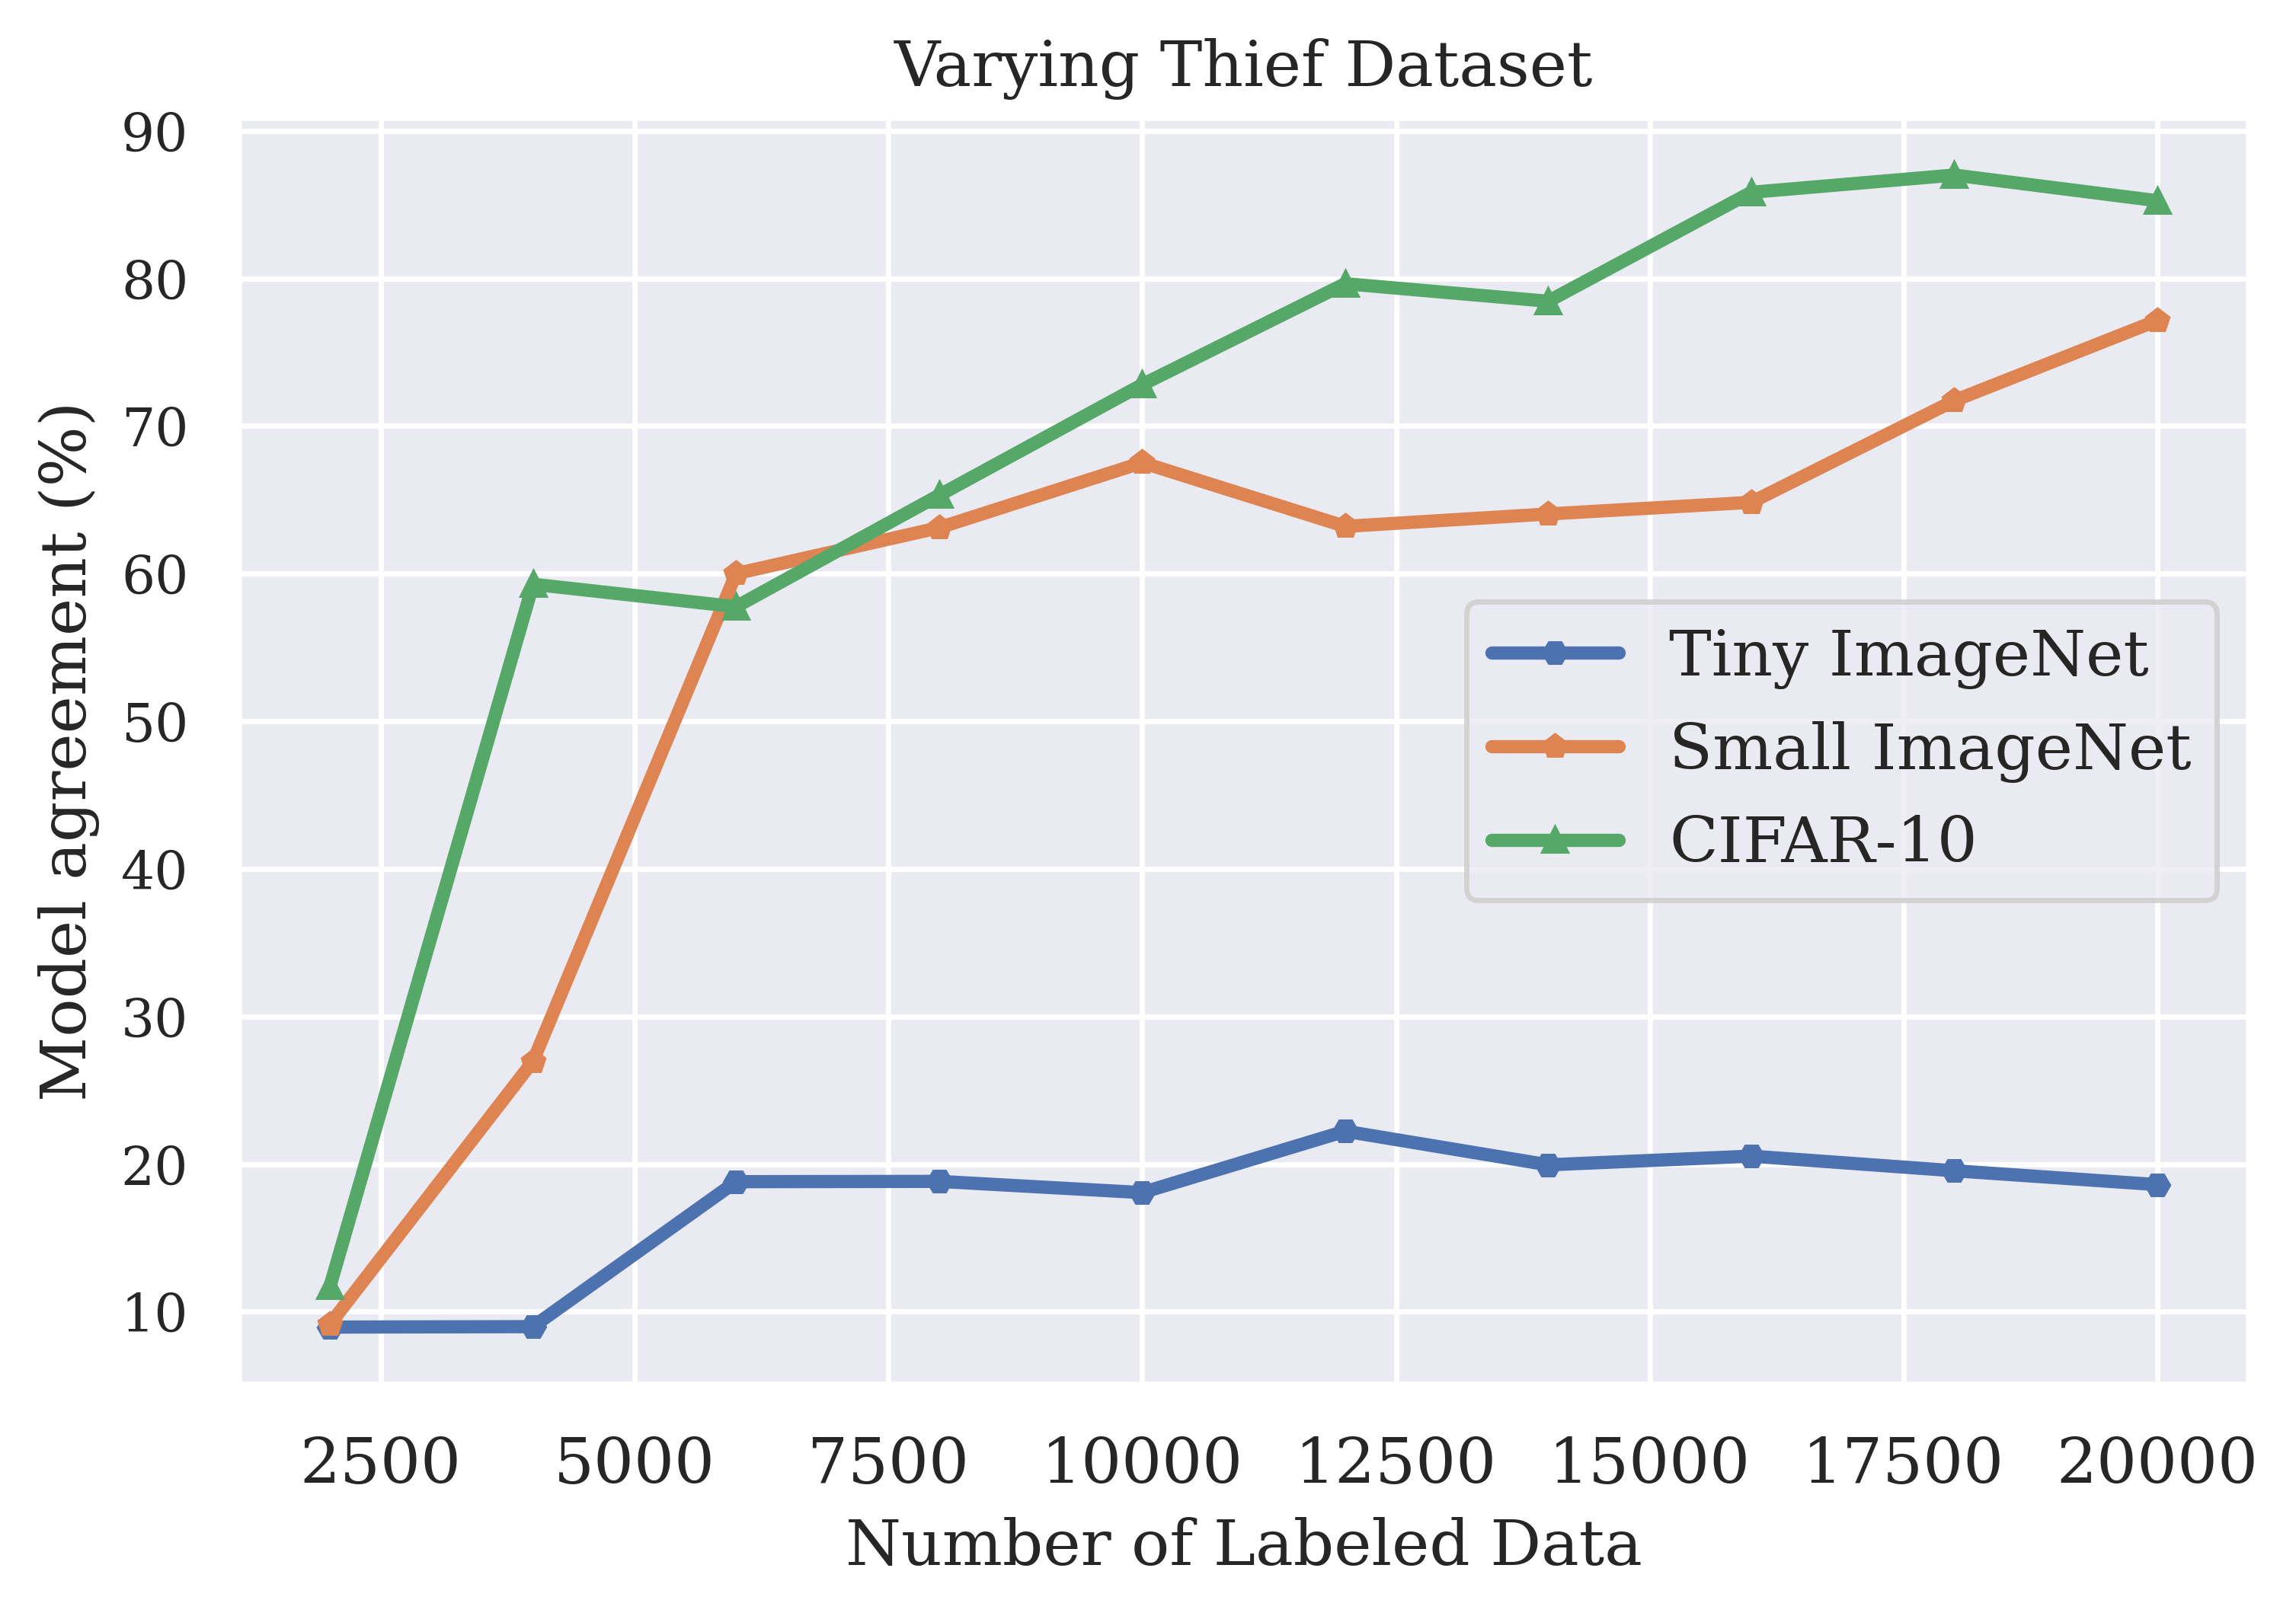
\includegraphics[width=0.8\linewidth]{images/results_CALMS/effect_dataset.png}
    \caption[Effect of Thief Dataset choice on the success of Model Stealing Attacks]{Comparison of Model Agreement when performing a model stealing attack using the datasets Tiny Imagenet, Small ImageNet and CIFAR-10. We perform Active Learning using the 
    straegy CoreSet with a batch size of 2000 for the experiments. The target model dataset used is MNIST.s}
    \label{fig:Evaluation:Results:CAL:EffectDataset}
\end{figure}


\subsubsection{Model Stealing Attacks using Continual Active Learning}
\label{sec:Evaluation:Results:MS:CAL}

In this section, we evaluate the success of Model Stealing Attacks using Continual Active Learning. More specifically, we run Model Stealing Attacks with Continual Active Learning on the datasets MNIST, CIFAR-10 and CIFAR-100, using the Active Learning strategies
Random, \gls{lc}, \gls{bald}, \gls{badge} and CoreSet and the Continual Learning strategies Naive, \gls{ewc}, \gls{imm}, \gls{mas} and \gls{alasso}. Furthermore, we differentiate between receiving the softmax output of the target model and solely receiving the top1-label. We use the ActiveThiefConv3 model
as the target and substitute model and perform one model stealing attack for each combination of Active Learning, Continual Learning strategy and target model output. For the baseline runs, we use a batch size of 1000 with a total query budget of 20000. The query budget
is kept for the Continual Active Learning runs, but we increase the batch size to 2000. The numbers reported in the table represent the model agreement at the end of each experiment, i.e. after using up the query budget of 20000. Readers interested in the progression of the
model agreement across the experiments can find the respective plots in appendix \ref{sec:Appendix:Results}. As a baseline we use the Model Extraction using Active Learning with the strategies mentioned before. To evaluate both the Active Learning strategies and the Continual
Learning strategies, we compute the average over the model agreement of all Continual Learning strategies combined with a fixed Active Learning strategy and the average of all Active Learning strategies combined with a fixed Continual Learning strategy. These numbers are given
at the end of each column and row, respectively. The Active Learning strategy and the Continual Learning strategy with the highest average model agreement are highlighted in bold. \par
In the first set of experiments, we perform Model Stealing Attacks using Continual Active Learning with MNIST as our target model and train the substitute model on the softmax output of the target model. The results of this experiment can be found in table
\ref{fig:ModelStealingMNISTSoftmax}. In terms of model agreement, all Continual Active Learning attacks perform significantly worse than the baseline. The best performing attack is the combination of the Active Learning strategy \gls{bald} with the Continual Learning strategy
\gls{mas} with a model agreement of 67.84\% after a query budget of 20000. The best performing Active Learning strategy is \gls{bald} with an average model agreement of 52.52\% across all Continual Learning strategies whereas the best Continual Learning strategy is \gls{mas} with an average
model agreement of 57.73\%. While the Continual Learning strategies struggled to outperform the Naive approach in the classic Continual Active Learning setting, most of them outperform the Naive approach in the Model Stealing setting. The only exception to this is \gls{alasso} which
falls behind the other approaches significantly. \par 

\begin{table}[h]
    \centering
    \begin{tabular}{c | c c c c c | c } 
        \hline
        \diagbox[width=11em]{Active \\ Learning Strategy}{Continual Learning \\ Strategy} & Random & \gls{lc} & \gls{bald} & CoreSet & \gls{badge} & $\varnothing$\\ 
        \hline 
        Baseline & 87.91 & 82.39 & 83.64 & 91.22 & 79.68 & 84.97\\
        \hline
        Naive & 47.74 & 43.02 & 59.61 & 58.36 & 48.89 & 51.52\\
        \gls{ewc} &  59.26 & 53.67 & 59.18 & 56.13 & 50.28 & 55.7\\
        \gls{imm} & 48.18 & 62.95 & 49.71 & 63.43 & 58.76 & 56.61 \\
        \gls{mas} &  64.42 & 50.27 & 67.84 & 55.58 & 50.54 & \textbf{57.73}\\
        \gls{alasso} & 28.04 & 15.5 & 26.28 & 10.39 & 12.8 & 20.6\\
        \hline
        $\varnothing$ & 49.57 & 45.08 & \textbf{52.52} & 48.78 & 44.24 & \\
        \hline
    \end{tabular}
    \caption[Model agreement of Continual Learning strategies on MNIST using softmax output]{Comparison of Model Agreement (in \%) for Model Stealing Attacks using Continual Active Learning on the MNIST dataset. We use Model Stealing Attacks with Active Learning as a baseline.
    In this set of experiments, we use the softmax output of the target model to train the substitute model.}
    \label{fig:ModelStealingMNISTSoftmax}
\end{table}

Next, we change the output of the target model to solely return the top1-label and perform the same set of experiments. Table \ref{fig:ModelStealingMNISTLabel} shows the results of these experiments. While the model agreement compared to training with softmax output of the
target model has dropped significantly for the baseline strategies, we do not observed a similar phenomenon for the Continual Active Learning strategies. Nevertheless, we observe a large maring between the Model Agreement of the Active Learning strategies and the Model Agreement
of the Continual Active Learning strategies. However, the combination of \gls{bald} and Naive comes close to its baseline, demonstrating a Model Agreement of 69.18\% which is about 7 percentage points lower than the respective baseline. Overall, the Naive approach performs best with an
average Model Agreement of 51.29\% across all Active Learning strategies. Contrary to the previous setup, no Continual Learning strategy outperforms the Naive approach, with \gls{mas} coming closest. The best Active Learning strategy is \gls{bald} with an average Model Agreement of 55.73\%. \par 

\begin{table}[h]
    \centering
    \begin{tabular}{c | c c c c c | c} 
        \hline
        \diagbox[width=11em]{Active \\ Learning Strategy}{Continual Learning \\ Strategy} & Random & \gls{lc} & \gls{bald} & CoreSet & \gls{badge} & $\varnothing$ \\ 
        \hline 
        Baseline & 67.56 & 80.36 & 76.29 & 81.62 & 76.43 & 76.45\\
        \hline
        Naive & 43.44 & 58.84 & 69.18 & 44.88 & 40.12 & \textbf{51.29}\\
        \gls{ewc} &  46.76 & 47.3 & 52.36 & 36.84 & 44.73 & 45.6\\
        \gls{imm} & 47.07 & 10.43 & 58.71 & 51.0 & 47.0 & 42.84\\
        \gls{mas} & 50.52 & 46.79 & 49.51 & 44.96 & 49.47 & 48.25\\
        \gls{alasso} &  10.44 & 46.89 & 48.89 & 16.27 & 10.43 & 26.68\\
        \hline
        $\varnothing$ & 39.65 & 50.97 & \textbf{55.73} & 38.79 & 38.35\\
        \hline
    \end{tabular}
    \caption[Model agreement of Continual Learning strategies on MNIST using the predicted class label]{Comparison of Model Agreement (in \%) for Model Stealing Attacks using Continual Active Learning on the MNIST dataset. We use Model Stealing Attacks with Active Learning as a baseline.
    In this set of experiments, we use the predicted label of the target model to train the substitute model.}
    \label{fig:ModelStealingMNISTLabel}
\end{table}

We move on to the next dataset which is CIFAR-10. First, we perform Model Stealing attacks using the softmax output of the target model. Our results can be found in Table \ref{fig:ModelStealingCIFAR10Softmax}. Similar to our findings from the MNIST dataset, the Continual Active Learning
are outperformed by the Active Learning strategies, however the gap between is mostly consistent across combinations of Active and Continual Learning strategies at around 10 percentage points. \gls{alasso} is once again an exception to this, performing significantly worse than the other
Continual Learning strategies. The best Continual Active Learning strategy is \gls{ewc} with an average Model Agreement of 60.14\%. At the same time, \gls{ewc} is the only Continual Learning strategy to outperform the Naive approach, albeit the margin between the two is only 0.48 percentage points.
Overall, CoreSet is the most performant Active Learning strategy with an average model agreement of 54.12\% across all Continual Learning strategies. \par

\begin{table}[h]
    \centering
    \begin{tabular}{c | c c c c c | c} 
        \hline
        \diagbox[width=11em]{Active \\ Learning Strategy}{Continual Learning \\ Strategy} & Random & \gls{lc} & \gls{bald} & CoreSet & \gls{badge} & $\varnothing$\\ 
        \hline 
        Baseline & 71.58 & 70.04 & 71.96 & 71.45 & 71.44 & 71.29\\
        \hline
        Naive & 60.8 & 56.62 & 61.84 & 61.61 & 57.42 & 59.66 \\
        \gls{ewc} & 58.67 & 56.8 & 61.57 & 61.79 & 61.88 & \textbf{60.14}\\
        \gls{imm} & 60.78 & 52.24 & 60.32 & 61.39 & 56.98 & 58.34 \\
        \gls{mas} & 50.32 & 51.45 & 52.09 & 52.23 & 55.68 & 52.35\\
        \gls{alasso} & 17.26 & 24.87 & 28.24 & 33.59 & 32.93 & 27.38\\
        \hline
        $\varnothing$ & 49.57 & 48.4 & 52.81 & \textbf{54.12} & 52.98\\
        \hline
    \end{tabular}
    \caption[Model agreement of Continual Learning strategies on CIFAR-10 using softmax output]{Comparison of Model Agreement (in \%) for Model Stealing Attacks using Continual Active Learning on the CIFAR-10 dataset. We use Model Stealing Attacks with Active Learning as a baseline. In this set of experiments,
    we use the softmax output of the target model to train the substitute model.}
    \label{fig:ModelStealingCIFAR10Softmax}
\end{table}

In our next experiment setup, we use the predicted label of the target model to train the substitute model, again with CIFAR-10 as the target model dataset. We present the results of this set of experiments in Table \ref{fig:ModelStealingCIFAR10Label}. Overall,
the Model Agreement is lower than when training with the softmax output of the target model, which is in line with the experiments conducted on the MNIST dataset. The gap between the baseline and the Continual Learning strategies has remained the same however,
resting at around 10 percentage points. \gls{ewc} is again the best performing Continual Learning strategy, outperforming the Naive approach by a large margin this time around. \gls{imm} follows closely, also beating the Naive approach. The main reason for the large gap
between the Naive approach and \gls{ewc} as well as \gls{imm} is the poor performance of \gls{bald} and Naive. Surprised by the poor performance of this combination, we run it again and find that the results are consistent. \gls{mas} and \gls{alasso}, on the other hand, do not manage to
outperform the Naive approach. In terms of Active Learning strategies, CoreSet performs best with an average Model Agreement of 43.57\% across all Continual Learning strategies. \par

\begin{table}[h]
    \centering
    \begin{tabular}{c | c c c c c | c} 
        \hline
        \diagbox[width=11em]{Active \\ Learning Strategy}{Continual Learning \\ Strategy} & Random & \gls{lc} & \gls{bald} & CoreSet & \gls{badge} & $\varnothing$\\ 
        \hline 
        Baseline & 60.23 & 49.73 & 61.28 & 63.78 & 62.26 & 59.46\\
        \hline
        Naive & 49.84 & 30.03 & 10.18 & 48.44 & 45.25 & 36.75\\
        \gls{ewc} & 50.37 & 47.12 & 50.22 & 47.94 & 49.11 & \textbf{48.95} \\
        \gls{imm} & 49.84 & 44.25 & 43.55 & 49.64 & 48.22 & 47.1\\
        \gls{mas} & 45.76 & 33.27 & 36.87 & 39.98 & 40.24 & 32.02\\
        \gls{alasso} & 19.05 & 38.16 & 30.91 & 31.86 & 25.04 & 29.0\\
        \hline
        $\varnothing$ & 42.97 & 38.57 & 34.35 & \textbf{43.57} & 41.57\\
        \hline
    \end{tabular}
    \caption[Model agreement of Continual Learning strategies on CIFAR-10 using the predicted class label]{Comparison of Model Agreement (in \%) for Model Stealing Attacks using Continual Active Learning on the CIFAR-10 dataset. We use Model Stealing Attacks with Active
    Learning as a baseline. In this set of experiments, we use the predicted label of the target model to train the substitute model.}
    \label{fig:ModelStealingCIFAR10Label}
\end{table}

The final target model dataset which we test for our setup is CIFAR-100. Like in the previous experiments, we first test all combination of Continual and Active Learning strategies trained on the softmax output of the target model
and compare them to the baseline of Active Learning. An exception to this are all experiments involving the Active Learning strategy \gls{badge}. We found the estimated runtime of \gls{badge} using ActiveThiefConv as our substitute model and SmallImagenet as our thief dataset
to be in excess of 40 days on our hardware, which is why we were unable to deliver results for this combination. The results for the remaining combinations from this set of experiments can be found in table \ref{fig:ModelStealingCIFAR100Softmax}.
Across the board, Model Agreement is significantly lower than in our previous experiments. The gap between the baseline and the Continual Learning strategies has decreased in absolute terms but increased in relative terms. Like in our previous experiments, \gls{ewc} outperforms
the remaining Continual Learning strategies, and it is one of two Continual Learning strategies which manage to outperform the Naive approach. The other strategy is \gls{imm}, which puts on a performance in between \gls{ewc} and the Naive approach. \gls{mas} follows behind the Naive approach
and \gls{alasso} is left behind once again. The best Active Learning strategy is CoreSet, which outperforms \gls{bald} by 0.57 percentage points. \par

\begin{table}[h]
    \centering
    \begin{tabular}{c | c c c c | c} 
        \hline
        \diagbox[width=11em]{Active \\ Learning Strategy}{Continual Learning \\ Strategy} & Random & \gls{lc} & \gls{bald} & CoreSet & $\varnothing$\\ 
        \hline 
        Baseline & 25.43 & 26.92 & 28.01 & 27.48 & 26.96 \\
        \hline
        Naive & 18.46 & 18.48 & 16.8 & 17.69 & 17.86\\
        \gls{ewc} & 19.45 & 17.46 & 20.67 & 19.98 & \textbf{19.39}\\
        \gls{imm} & 18.16 & 17.9 & 20.39 & 18.75 & 18.8\\
        \gls{mas} & 15.75 & 14.85 & 14.72 & 15.45 & 15.19\\
        \gls{alasso} & 5.2 & 4.95 & 6.7 & 10.24 & 6.77\\
        \hline
        $\varnothing$ & 15.4 & 14.73 & 15.85 & \textbf{16.42}\\
        \hline
    \end{tabular}
    \caption[Model agreement of Continual Learning strategies on CIFAR-100 using softmax output]{Comparison of Model Agreement (in \%) for Model Stealing Attacks using Continual Active Learning on the CIFAR-100 dataset. We use Model Stealing Attacks with Active Learning as a baseline.
    In this set of experiments, we use the softmax output of the target model to train the substitute model.}
    \label{fig:ModelStealingCIFAR100Softmax}
\end{table}

Finally, we compute the Model Agreement across multiple combinations of Continual Learning and Active Learning strategies using the predicted label of the target model and CIFAR-100 as our target model dataset. As in the previous set of experiments, we omit the results of
the Active Learning strategy \gls{badge}. Compared to training on the softmax output of the target model, the model agreement has disproportionally decreased for the Continual Learning strategies. While the baseline strategies boast a Model Agreement of 20.42\% on average, the
best Continual Learning strategy, which is \gls{imm}, manages to achieve a Model Agreement of 8.07\% on average. \gls{imm} significantly outperforms both the Naive approach and \gls{ewc}, which demonstrate almost identical performance. We were surprised by the poor performance of \gls{ewc} and \gls{bald},
which is why we conducted this experiment one more time, however we achieved similar results. The remaining Continual Learning strategies, \gls{mas} and \gls{alasso}, perform worse than the Naive approach. Remarkably, \gls{alasso} outperforms \gls{mas}, making this the only set of experiments in which
\gls{alasso} is not the worst performing Continual Learning strategy. Another surprise is the performance of the Random Active Learning strategy, which outperforms the remaining Active Learning strategies. CoreSet, which demonstrated strong performance in previous experiments, falls behind
Random and \gls{lc}, outperforming only \gls{bald} by about one percentage point. \par

\begin{table}[h]
    \centering
    \begin{tabular}{c | c c c c | c} 
        \hline
        \diagbox[width=11em]{Active \\ Learning Strategy}{Continual Learning \\ Strategy} & Random & \gls{lc} & \gls{bald} & CoreSet & $\varnothing$\\ 
        \hline 
        Baseline & 21.65 & 19.5 & 19.64 & 20.9 & 20.42\\
        \hline
        Naive & 7.93 & 7.63 & 4.98 & 4.82 & 6.34\\
        \gls{ewc} & 8.79 & 6.55 & 2.07 & 7.77 & 6.3\\
        \gls{imm} & 8.59 & 8.44 & 7.18 & 8.05 & \textbf{8.07}\\
        \gls{mas} & 5.37 & 5.44 & 5.3 & 4.52 & 5.16\\
        \gls{alasso} & 5.28 & 6.11 & 5.72 & 5.51 & 5.66\\
        \hline
        $\varnothing$ & \textbf{7.19} & 6.83 & 5.05 & 6.13 \\
        \hline
    \end{tabular}
    \caption[Model agreement of Continual Learning strategies on CIFAR-100 using the predicted class label]{Comparison of Model Agreement (in \%) for Model Stealing Attacks using
    Continual Active Learning on the CIFAR-100 dataset. We use Model Stealing Attacks with Active Learning as a baseline. In this set of experiments,
    we use the predicted label of the target model to train the substitute model.}
    \label{fig:ModelStealingCIFAR100Label}
\end{table}

After having conducted our experiments with the Continual Learning strategies Naive, \gls{ewc}, \gls{mas}, \gls{imm} and \gls{alasso} as well as the Active Learning strategies
Random, \gls{bald}, \gls{lc}, CoreSet and \gls{badge}, we test the combination of the Active Learning strategy \gls{vaal} with the Continual Learning strategy \gls{a-gem}. We motivate
this experiment by the performance of \gls{vaal} and \gls{a-gem} in the classic Continual Learning setup, given in Figure \ref{sec:Evaluation:Results:CAL:VAAL_AGEM}.
The experiments are performed in the same manner as the previous experiments in this section. To evaluate the performance of \gls{vaal} and \gls{a-gem}, we compare
the results to the best performing Active Learning strategy, CoreSet, and the combination of the best performing Continual Learning strategy and the
most performant Active Learning strategy, which are \gls{ewc} and CoreSet, respectively. The results of the comparison are given in Table 
\ref{fig:ModelStealingVAALAGEM}. We present the progression in Model Agreement with \gls{vaal} and \gls{a-gem} in Appendix \ref{sec:Appendix:Results}. While \gls{vaal}
and \gls{a-gem} cannot keep up with the performance of the baseline, just as all Continual Active Learning approaches, it performs on par with CoreSet and \gls{ewc},
outperforming them in 3 out of 6 experiments while being outperformed in the remaining 3 experiments. \par
\begin{table}[h]
    \centering
    \begin{tabular}{c c c c c c c} 
        \hline
        & \multicolumn{2}{c}{MNIST} & \multicolumn{2}{c}{CIFAR-10} & \multicolumn{2}{c}{CIFAR-100} \\ 
        \cline{2-7} Attack strategy & Softmax & Label & Softmax & Label & Softmax & Label \\
        \hline 
        \gls{vaal} \gls{a-gem} & 52.54 & 53.8 & 61.48 & 50.5 & 18.29 & 8.77\\
        CoreSet \gls{ewc} & 56.13 & 36.84 & 61.79 & 47.94 & 19.98 & 7.77 \\
        Coreset Baseline & 90.65 & 77.58 & 71.61 & 61.68 & 27.52 & 20.96\\
        \hline
    \end{tabular}
    \caption[Comparison of Model Agreement using \gls{vaal} and \gls{a-gem}]{Comparison of Model Agreement (in \%) for Continual Active Learning using \gls{vaal}
     and \gls{a-gem}, CoreSet and \gls{ewc} as well as the CoreSet Baseline}
    \label{fig:ModelStealingVAALAGEM}
\end{table}

We close the evaluation section with a surprising finding regarding the effect of data augmentation on the success of Model Stealing Attacks. While
we managed to reproduce the findings of Pal et al. for CIFAR-10, we failed to do so for MNIST. Since multiple training hyperparameters of the experiments
presented in ActiveThief were not disclosed by the authors, we experiment with different combinations of hyperparameters, including varying the optimizer,
the learning rate, the number of training epochs, the batch size and switching between cold start and warm start for Active Learning. Sadly, we were still
not able to reproduce the results of ActiveThief on MNIST. After conducting the experiments presented above, we decided to investigate another hyperparameter:
training with or without data augmentation. For this set of experiments, we leave all hyperparameters equal to the previous experiments, apart from the data
augmentation. It is important to note here that we do or do not use data augmentation on the thief dataset, not on the target model dataset. Training the
target model is always done using data augmentation. We perform the same model stealing attacks as before, using MNIST and CIFAR-10 as target model dataset
and present the results in figure \ref{fig:Evaluation:Results:CAL:EffectAugmentation}. When performing Model Stealing Attacks without data augmentation on
CIFAR-10, we notice that Model Agreement, both for Active Learning and Continual Active Learning, is significantly lower than when using data augmentation.
In this scenario, Continual Active Learning with data augmentation performs on par with Active Learning without data augmentation. However, when using MNIST
as target model dataset, the results are reversed. Here, Model Agreement is significantly lower when using data augmentation. More importantly Continual
Active Learning without data augmentation shows performance comparable to Active Learning with data augmentation. \par

\begin{figure}[h]
    \centering
    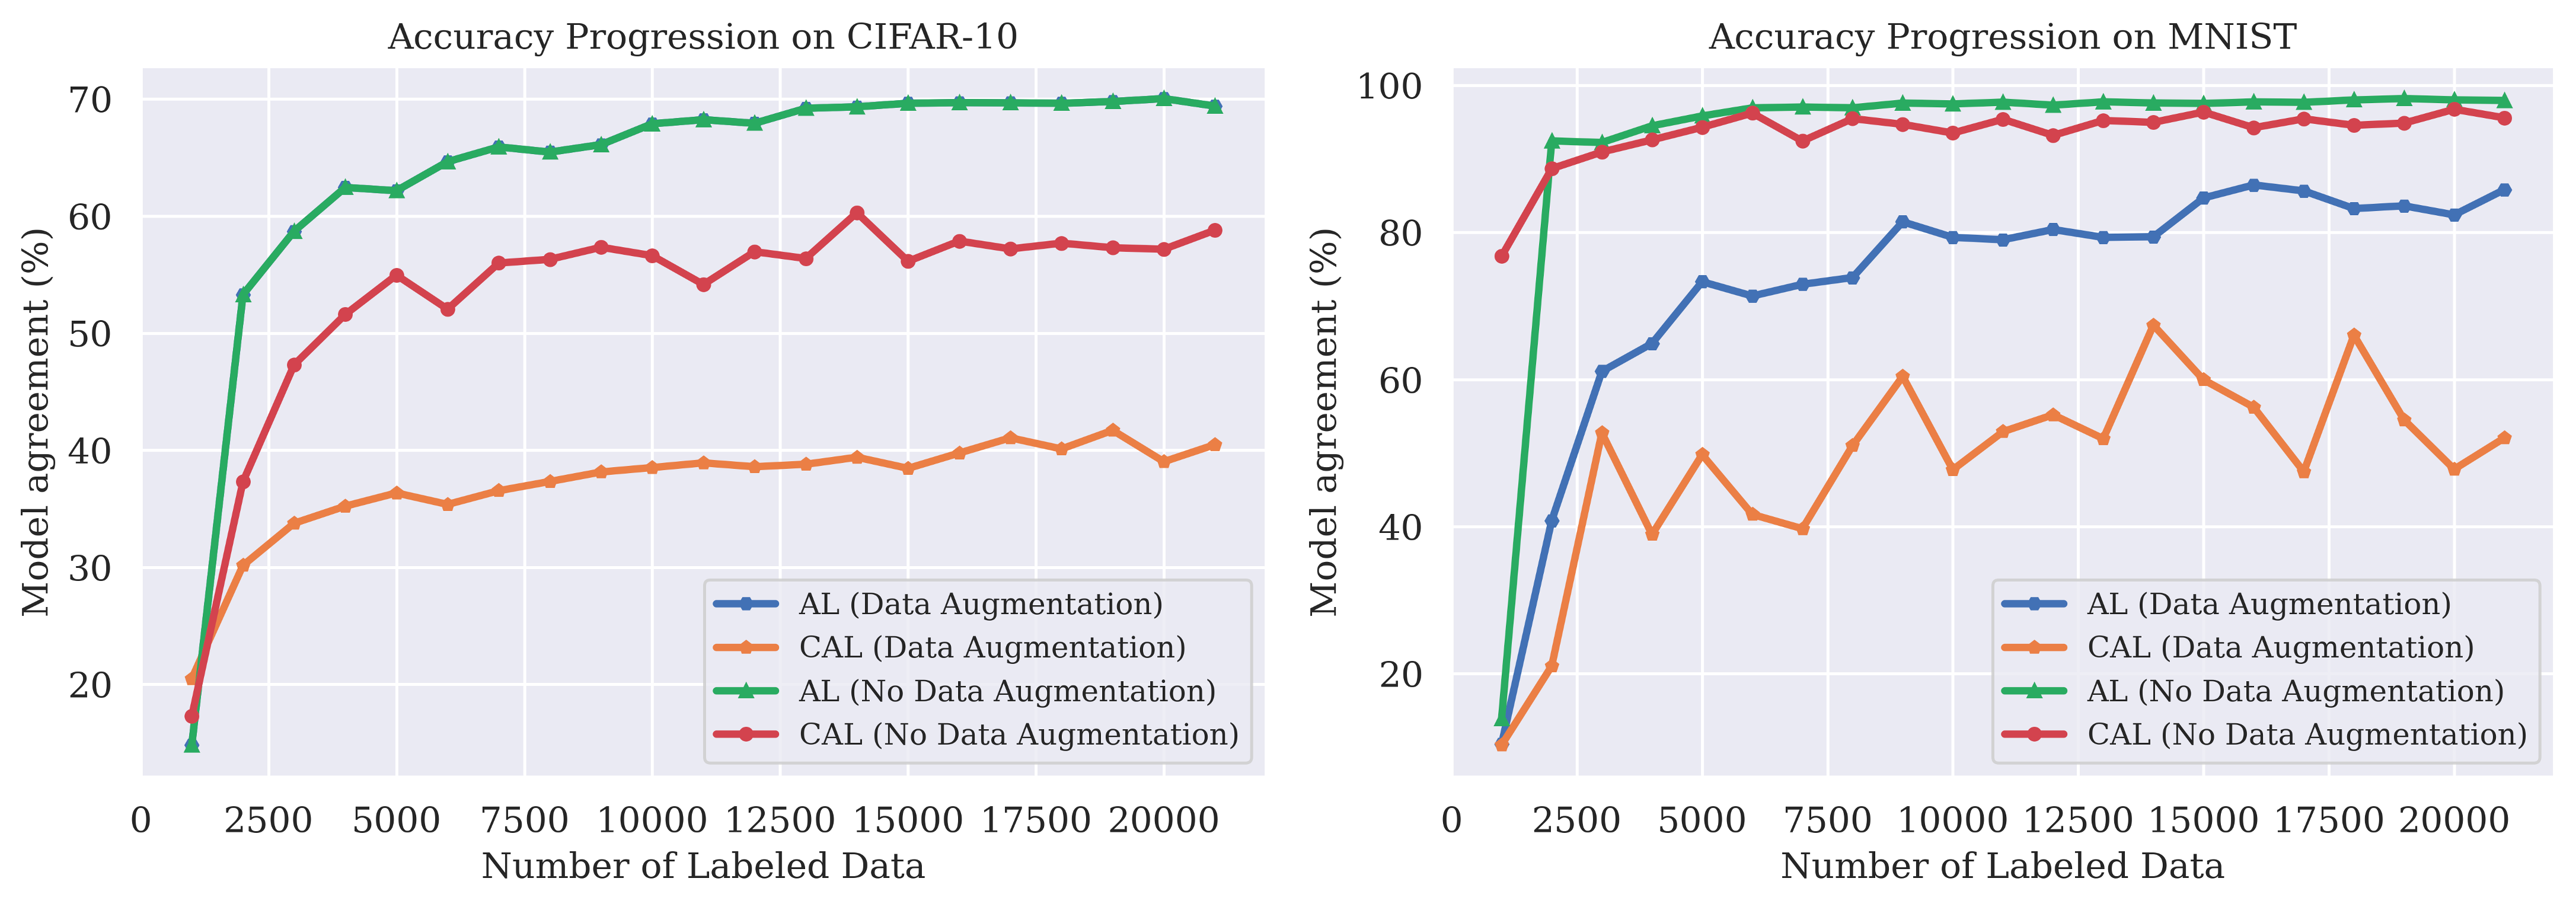
\includegraphics[width=\linewidth]{images/results_CALMS/effect_data_augmentation.png}
    \caption[Effect of Data Augmentation on the success of Model Stealing Attacks]{Comparison of Model Agreement when using different data augmentation
    techniques. For Active Learning we use a batch size of 1000 and for Continual Active Learning we use a batch size of 2000. Left: Experiments with
    the target model dataset CIFAR-10. Right: Experiments with the target model dataset MNIST.}
    \label{fig:Evaluation:Results:CAL:EffectAugmentation}
\end{figure}

%% LaTeX2e class for student theses
%% sections/conclusion.tex
%% 
%% Karlsruhe Institute of Technology
%% Institute for Program Structures and Data Organization
%% Chair for Software Design and Quality (SDQ)
%%
%% Dr.-Ing. Erik Burger
%% burger@kit.edu
%%
%% Version 1.3.6, 2022-09-28

\chapter{Discussion}
\label{ch:Discussion}
% Was war das Ziel? Was wurde (nicht) erreicht?
In this chapter, we will discuss our findings from the experiments in chapter \ref{ch:Evaluation}. Like most chapters in this thesis, we will divide this chapter into two parts, one for continual active learning and one for model stealing. 
The first section will discuss the findings from the first batch of experiments, where we tested Continual Active Learning on the CIFAR-10 dataset using Resnet18. The section on Model Stealing is then used to discuss general findings from
our experiments on Model Stealing as well as findings from applying Continual Active Learning to Model Stealing. 

\section{Continual Active Learning}
\label{sec:Discussion:ContinualActiveLearning}
The goal of this section is to discuss the findings from section \ref{sec:Evaluation:Results:CAL}. When developing the Continual Active Learning approach proposed in this thesis, our initial aim was to improve both the overall performance, measured
by validation accuracy, of the model and the training time in comparison to Active Learning. By studying the results we observe that we were not able to outperform Active Learning in any of the experiments. On the contrary, Active Learning, even naive
Active Learning using random sampling, significantly outperforms Continual Active Learning in terms of validation accuracy. However, we managed to achieve the second goal of improving the training time. Before we analyze the reasons for the poor performance 
of Continual Active Learning in terms of validation accuracy, we will first discuss the performance in terms of execution time.

\subsection{Execution time}
\label{sec:Discussion:ExecutionTime}

In terms of training time, we observe that Continual Active Learning outperforms Active Learning in all experiments. The main reason for the superior performance of Continual Active Learning runtime-wise is that the model is trained on significantly less data
in the training process. In section \ref{sec:Methodology:CombiningCLandAL} we mentioned that a model trained with a total budget of $n$ and a batch size of $b$ is trained on $\frac{n(n+b)}{2b}$ data points. When we use this equation with the parameters given in
our experiments, namely $n=50000$ and $b \in \{ 1000, 2000, 4000\}$, we see that the total number of points trained increases almost proportionally with a decreasing batch size. This phenomenon is shown in table \ref{fig:NumberOfTrainingPoints}, where we computed
the total number of training points for the batch sizes used in the experiments. In our case, we train on almost four times as many data points when using a batch size of 1000 compared to a batch size of 4000. Since the total number of training points is constant
for Continual Active Learning with varying batch sizes, we do not observe the same phenomenon. \par

\begin{table}[h]
    \centering
    \begin{tabular}{| c | c |} 
        \hline
        $b$ & Total number of training points \\
        \hline 
        1000 & 1275000 \\
        2000 & 650000 \\
        4000 & 362000 \\
        \hline
    \end{tabular}
    \caption[Total number of data points trained on in the Continual Active Learning experiments]{Total number of training points for varying batch sizes on the CIFAR-10 dataset, which has a train set of consisting of 50000 elements.}
    \label{fig:NumberOfTrainingPoints}
\end{table}

The total number of training points perfectly explains the execution time of the Active Learning strategies Random and LC. In the experiments, the execution time of Random is at approximately 2500 Minutes for batch size 1000, 1300 for batch size 2000 and 700 for
batch size 4000 with LC showing comparable results. On the other hand the Continual Active Learning strategies using Random and LC show similar runtime for batch size 2000 and 4000 but the execution time for batch size 1000 is merely half the execution time when
using the previous batch sizes. This discrepancy in execution time can be explained by the number of epochs trained in each iteration of Active Learning. For batch size 1000, we train for 80 epochs per iteration while we train for 150 epochs per iteration for
batch size 2000 and 4000. \par
While we have analyzed how the runtime of LC and Random can be explained we still need to analyze the runtime of Badge, CoreSet and BALD. LC and Random have a very low query time, which is negligible with a dataset of the size of CIFAR-10 and a model like ResNet18.
In this specific setting BALD exhibits a runtime which is almost identical to LC and Random. This is because ResNet18 does not contain any dropout layers. Since our implementation of BALD dynamically detects whether the model contains dropout layers and only performs
Monte Carlo dropout if it does, we only run one dropout iteration in this setting. In theory, we could run multiple iterations of Monte Carlo dropout, however this increases query time, and runtime for that matter, without improving the performance of BALD. Using only
one dropout iteration in our setting is sufficient since the predictions of a Neural Network without activated dropout layers are deterministic. In general however, the query time of BALD depends on the number of dropout iterations, which is a hyperparameter, the size
of the unlabeled pool and the prediction speed of the model. \par
CoreSet and Badge are Active Learning strategies which incorporate diversity into their sampling. With CoreSet being entirely diversity-based and Badge being both diversity-based and uncertainty-based, these strategies compute a cover of the data points in the pool using
a k-center greedy algorithm and $k$-Means++ respectively. Both strategies use distance computation in their sampling which becomes more expensive computationally with an increasing number of data points and a larger feature space. This explains the higher query time of
CoreSet and Badge compared to LC, BALD and Random. Furthermore, it is worth noting that BALD and LC are rank-based, meaning that they always compute their respective importance measure for the complete unlabeled pool and then return the $b$ most informative data points
according to their importance measure. Therefore, a query with batch size $b_1$ while always be a subset of a query with batch size $b_2$ if $b_1 < b_2$. CoreSet and Badge on the other hand are not rank-based, meaning that they compute a cover of a feature space. The
optimal cover depends on the batch size. It is therefore theoretically possible that a query with batch size $b_1$ and a query with batch size $b_2$ have no data points in common, if $b_1 \neq b_2$. For CoreSet, and even more so for Badge, the query time becomes a
bottleneck in our experiments. While the total query time in our experiment is not dependent on the batch size, because we always query the complete train set over the course of the experiment, it is still a considerable portion of the total runtime. The main reason why
Continual Active Learning using Badge or CoreSet do not outperform the respective baseline by a factor as large as the one of Continual Active Learning straegies using BALD, LC or Random is that with increasing batch size the training time becomes a smaller fraction of
the execution time while the query time remains constant. \par
Next, we investigate the contribution of the Continual Learning strategies in terms of runtime. Overall, we observe that the overhead introduced by the Continual Learning strategies is negligible compared to the overhead introduced by the Active Learning strategies. The
biggest increase in runtime is caused by Alasso, which increases the execution time by 30 to 60 Minutes in our experiments. The reason for the increase in runtime is most likely the backpropagation step. Alasso needs two backward passes through the model to compute the
complete gradients: The first is used to compute the unregularized gradients which are needed for the computation of $\Omega$ in Equation \ref{eq:ALASSO_Omega} and the second is used to compute the gradients for the surrogate loss. MAS, IMM and EWC only need one backward
pass to compute the gradients, just as the Naive approach, because they do not require saving the unregularized gradients. \par
Apart from the overhead introduced by backpropagation, the Continual Learning strategies introduce overhead by estimating weights for the parameters of the Neural Network at the end of each task. Alasso computes its weights by using equation \ref{eq:ALASSO_Omega}, MAS
uses the gradients of the validation step whereas EWC and IMM compute the diagonals of the Fisher Information Matrix. Overall, this overhead is minimal however, as can be seen from the execution times presented in section \ref{sec:Evaluation:Results:CAL}. Surprisingly,
IMM and EWC demonstrate minimally lower runtime than the Naive approach in a few experiments. While this is not possible in theory because the Naive approach does not compute any importance weights, we believe that the superior performance of IMM and EWC when using LC,
IMM and BALD can be explained by factors that are beyond our control, such as operating system overhead or disk access speed. At this stage, we would like to point out that we do not intend to give a perfect ranking of the Continual Learning strategies in terms of
execution time, but we rather aim to give a rough estimation of the speedup introduced by using Continual Active Learning over Active Learning. For CoreSet and Badge, the difference in runtime between Naive, EWC and IMM can be explained by the fact that the query time
is not deterministic for these Active Learning strategies, because computing their query results requires computing a set cover like in CoreSet or a $k$-Means++ initialization like in Badge. \par
% Further explanations in terms of runtime: BALD and LC are rank based, i.e. their query time does not depend on the batch size. CoreSet and Badge are batch size dependent since they compute a cover of the data points and more data points means more points in the cover.
% For continual learning strategies mention that one overhead is the computation time during gradient computation which is needed for backpropagation and for some strategies the importance weights need to be computed.



% In terms of accuracy: mention that CAL does not work as expected because the CL strategies were not designed for the scenario which we are using them in, i.e. training on the same dataset. Mention that batch size plays a major role as can be seen from the experiments.
\subsection{Validation Accuracy}
\label{sec:Discussion:ValidationAccuracy}
After analyzing the results in terms of execution time, we will now focus on the validation accuracy. As mentioned before, the Continual Active Learning strategies are significantly outperformed by the Active Learning strategies in terms of validation accuracy. Before we
analyze the difference in performance between Active Learning and Continual Active Learning, we will first investigate them on their own. \par
When investigating the validation accuracy curves of the Active Learning strategies we see that, apart from random sampling, they allow follow the same pattern: First, the validation accuracy increases rapidly until the size of the labeled pool has reached about 20\% of
the full labeled set. When the labeled pool comprises 20\% to 50 \% of the full labeled set, the validation accuracy increases moderately until it reaches its peak at 50\% of the labeled set. Between 50\% and 100\% of the labeled set, the validation accuracy
decreases slightly until it reaches the level it achieved with 20\% of the full training set. Before we analyze why this behavior occurs, we point out that the batch size has a negligible effect on the validation accuracy progression in our experiments, which is in line
with the findings of Beck et al. \cite{beck2021effective}. The validation accuracy curve of Active Learning can be explained as follows: First, the model is trained on the most informative samples which leads to a rapid increase in validation accuracy. However, the larger
the size of the labeled pool, the less informative samples exist and the less informative are even the most informative samples of the unlabeled pool. This is the reason for the moderate increase in validation accuracy between 20\% and 50\% of the labeled pool. At the point
where the labeled pool comprises 50\% of the full labeled set, the model has seen all the informative samples and the validation accuracy starts to decrease as the newly labeled samples are uninformative. Nevertheless, the validation accuracy does not experience a sharp decline
because the labeled pool still contains the informative samples which where labeled in the beginning. \par
The validation accuracy curves of the Continual Learning strategies are more diverse than the ones of the Active Learning strategies. When analyzing these validation accuracy curves, it is important to keep in mind that a single Continual Active Learning strategy consists of a
combination of an Active Learning strategy and a Continual Learning strategy, and therefore we need to analyze the contribution of both the Active Learning strategy and the Continual Learning strategy to the validation accuracy. Since we used more than 25 combinations of Continual
and Active Learning strategies in our experiments, we will not be able to analyze each combination in detail. This is not necessary however, because the contribution of Active Learning and Continual Learning to the validation accuracy can be isolated mostly. \par
First, we will analyze the Contribution of the Continual Learning strategies on the validation accuracy of Continual Learning. We start off with Alasso, which is clearly demonstrates the most inferior performance of all Continual Learning strategies. A major problem of Alasso is
its erratic behavior. While Alasso does not perform significantly worse than the other Continual Learning strategies when the accuracy curves are averaged, it has by far the highest variance in its validation accuracy. Furthermore, the previous statement only holds for experiments
using a batch size of 1000. For batch size 2000 and 4000, Alasso becomes practically unusable after about 10000 samples because it shows a steady decline in validation accuracy. We believe that this is due to the fact that the overestimation of the loss on a single side of the 
loss function creates an uneven loss function. The problem is that overestimation is done on a per-parameter basis, meaning that the loss could be overestimated for one parameter and correctly estimated for another. The exploding gradient problem we observe in our experiments
supports the thesis that parameter optimization using gradient descent is hard when the loss is estimated as it is done with Alasso. While using gradient clipping did mitigate the exploding gradient problem, it did not solve it completely. When observing the loss progression for
Alasso, we notice that the loss dramatically increases for the first epoch of each Active Learning iteration. Subsequently, the loss decreases but is unable to recover from the gradient shift performed in the first epoch. We tried clipping the gradient at even smaller values of
the $l_2$-Norm to eradicate the loss increase in the first epoch, however this impeded model convergence. \par
Next, we will analyze IMM and EWC jointly. The reason for the joint analysis is that they perform on a comparable level and they both estimate parameter importance similarly. Overall, IMM and EWC demonstrate a validation accuracy that is on par with the Naive approach. We believe
that this is because they employ regularization less stringently than Alasso and MAS. This is supported by the experiments where the validation accuracy for Naive, IMM and EWC drops of similarly while MAS manages to maintain its validation accuracy. Our experiment with the delayed
start of Continual Active Learning in Figure \ref{fig:Evaluation:Results:CAL:DelayedStart} provides further evidence for this thesis. \par
Third, we investigate the behavior of MAS. MAS performs significantly better than Alasso in terms of validation accuracy but is outperformed by IMM, EWC and Naive. We believe that this is caused by the fact that MAS restricts parameter updates more than EWC and IMM. When observing
the validation accuracy progression of MAS, we note that MAS does not exhibit the steady increase in validation accuracy that EWC, IMM and Naive do, but it also does not experience the sharp decline in validation accuracy within the final 10000 samples. While it is desirable that
MAS effectively manages to preserve previously learn knowledge, we argue that it lacks the ability to adapt to new tasks. \par
Finally, we will analyze the Naive approach, which also enables us to bridge between the contribution of Continual Learning and Active Learning to the validation accuracy. The Naive approach performs significantly better than Alasso and MAS in the first 40000 samples, which is due
to the fact that it does not restrict parameter updates at all. Since the accuracy of the Naive approach increases for the first 25000 samples approximately, we assume that these samples are the ones that are informative enough to further make the model further learn the task it is
trained for. After about 20000-30000 samples the accuracy of the Naive approach starts to decline, which is caused by the fact that the samples in this period are less informative than before, although they are still informative enough to impede forgetting. The final 5000 samples how-
ever introduce a significant reduction in validation accuracy which is interesting because it demonstrates that a task can be unlearned to some extent when using data that belongs to the very same task. \par
Moving on to the contribution of Active Learning to the validation accuracy, we first analyze the performance of the Active Learning strategy LC. Continual Active Learning strategies using LC generally follow the pattern described in the previous section. To add to the previous
section, we believe that for LC the drop in validation accuracy within the final 10000 samples of the experiments is caused by an uneven class distribution in the final queries. We observed the class distribution for LC over multiple iterations and noticed that it became increasingly
inhomogeneous over time. \par
Next, we investigate the contribution of BALD to the validation accuracy of Continual Active Learning. We note that there is a large variance in the validation accuracy, especially when using a batch size of 1000. With larger batch sizes, the variance in validation accuracy decreases
but BALD is still not able to demonstrate comparable performance with other Active Learning strategies. This is due to the special circumstances of the experiment setup. Since we use ResNet18, which does not contain dropout layers, we are unable to run Monte Carlo dropout to accurately
estimate $\mathbb{E}_{\theta \sim p(\theta \mid L)} [H[y \mid x, \theta]]$. \par
Regarding Badge and CoreSet, we notice that their show matching performance, similar to EWC and IMM in the Continual Learning setting. Badge and CoreSet follow the typical Continual Active Learning curve, described in the paragraph for the Naive strategy, the most. This is due to the
fact that they incorporate diversity into their sampling strategies which smooths the validation accuracy curve except for the final 5000 samples and experiments with batch size 10000. We believe that the final 5000 samples generally do not represent the task the model is trained for
well and therefore even a subset that is representative of these samples cannot be used to improve the validation accuracy. For the setting with 1000 batch size, the issue is rather that these 1000 points are not enough to represent the unlabeled pool well. \par
Finally, we briefly discuss the performance of VAAL and A-GEM. VAAL as an Active Learning strategy by itself is outperformed by the remaining Active Learning strategies which demonstrates that is unable to select the most informative samples to query. However, this is an advantage when
using VAAL in conjunction with A-GEM. In our experiment with LC and A-GEM, we noticed that A-GEM outperformed LC in terms of validation accuracy within the first 15000 samples but suffered from a heavy drop in validation accuracy thereafter. It seems that A-GEM struggles to retain the
knowledge of previously learned samples when their informativeness changes rapidly. Ironically, the fact that VAAL is not as performant as the other Active Learning strategies helps A-GEM increase its validation accuracy when combined with VAAL. \par

We close this section by aiming to answer the most important question: Why does Continual Active Learning not outperform Active Learning? We believe that this is mainly due to the number of training points being used in each iteration. While Active Learning strategies use the
complete labeled pool in each iteration ($i \cdot b$ data points where $i$ is the number of iterations), Continual Active Learning strategies only use the data points that have been labeled in the current task, i.e. $b$ points. It is worth pointing out that the correlation between
data points trained on, and validation accuracy achieved is not perfect by any means. However, especially if the number of data points trained on is less than 20\% of the full size of the training set, just one or two percentage points can make a big difference in terms of validation
accuracy. This is supported by the observation that the validation accuracy increases with an increasing batch size. Our Replay strategy further demonstrates this behavior. For varying sizes of the replay buffer and the batch size, we observe identical performance as long as the sum
of replay buffer size and batch size is identical. Analysis of the second experiment with our Replay strategy shows that for the first 25000 samples, it is irrelevant how we select the data we replay, which further supports the thesis. \par
A second component to the answer of the question is the fact that the Continual Learning strategies we used, or any Continual Learning strategy for that matter, are not designed for a setting in which all the training data belong to the same task. The Continual Learning strategies have
been developed for and evaluated on task-incremental and class-incremental learning settings.


\section{Model Stealing}
\label{sec:Discussion:ModelStealing}
In this section we will discuss the results of the experiments which involve Model Stealing, i.e. the experiments conducted in section \ref{sec:Evaluation:Results:MS:CAL}. First, we will analyze the general observations regarding Model Stealing attack which we made and compare them
to the findings of Pal et al. in ActiveThief as well as Orekondy et al. in Knockoff Nets. Next, we will elaborate on the results of our Continual Active Learning Attacks strategy for Model Stealing Attacks.

\subsection{General Model Stealing Observations}
\label{sec:Discussion:ModelStealing:General}
We make three decisive observations for Model Stealing which we will present in this subsection. The first observation is that the success of a Model Stealing Attack, which is measured by Model Agreement in our case, is highly dependent on the thief dataset. From our experiment in 
Figure \ref{fig:Evaluation:Results:CAL:EffectDataset}, we see that the Model Agreement at the end of the attack is approximately 85\% for CIFAR-10, 80\% for Small ImageNet and merely 20\% for Tiny ImageNet. While previous works such Knockoff Nets state that \enquote{any large diverse set
of images makes for a good transfer set}, we come to a different conclusion. Tiny ImageNet consists of 100000 images which should be enough to steal a model trained on a simple dataset like MNIST is. The strong performance of CIFAR-10 in this experiment contradicts the claims from
Orekondy et al. even more because CIFAR-10 is arguably less diverse than Tiny ImageNet but significantly outperforms it in this setting. \par
The second observation we make is that the success of a model stealing does depend on the architecture of both target and substitute model. In our experiments, ActiveThiefConv3 and ActiveThiefConv4 perform significantly better than ActiveThiefConv2 when being used as a target model
and on the other hand, model stealing attacks extracting ActiveThiefConv2 achieve higher Model Agreement than those extracting ActiveThiefConv3 or ActiveThiefConv4. This is in line with the findings of Orekondy et al. while it contradicts the findings of Pal et al. We do note however,
that Pal et al. most likely compared Model Agreement between Neural Network architectures when training on the full thief datasets where we compared Model Agreement after using Active Learning for Model Extraction with a total budget of 20000. We believe that our findings are more
representative because they do not assume training on a full dataset. \par
Finally, we observed that data augmentation can significantly effect the success of Model Stealing attacks. Unfortunately however, there is no general rule whether data augmentation is beneficial or not. In our experiments with MNIST as target model dataset, we observed that
renouncing data augmentation significantly increased Model Agreement whereas the opposite was the case for CIFAR-10 as target model dataset. We believe that learning to classify MNIST is a much easier task than learning to classify CIFAR-10 and therefore, using data augmentation
when extracting a model trained on MNIST only obscures the function learned by the target model. Since most real world datasets are more similar to CIFAR-10 than to MNIST, we believe that performing data augmentation on the thief dataset generally is beneficent for Model Stealing
in the real world. The effect of data augmentation proves another point however: Model Stealing is a domain where a single hyperparameter can have a significant effect on the outcome of an experiment.

\subsection{Continual Active Learning for Model Stealing}
\label{sec:Discussion:ModelStealing:CALMS}
Next, we will turn to the results of the experiments where we applied Continual Active Learning to perform Model Stealing Attacks. We will discuss the results on the three different target model datasets separately and then mention any findings that apply to all three datasets. \par
Regarding our experiment for the MNIST dataset, we notice that the gap in performance of Continual Active Learning to Active Learning is even larger than in the classic Continual Active Learning setting, both when training using the softmax output of the target model and when using 
only the predicted class label. We assume that the main reason for the poor performance of Continual Active Learning in this setting is the fact that we used data augmentation for the thief dataset. In Figure \ref{fig:Evaluation:Results:CAL:EffectAugmentation} we presented the results
of our experiments performing Model Stealing with and without data augmentation on the thief dataset. We see that for the MNIST dataset, renouncing data augmentation significantly increases Model Agreement. When using data augmentation with MNIST as target model dataset, it is more
challenging to learn the function of the target model, especially when training solely on 2000 data points at a time. \par
For the CIFAR-10 dataset, we noticed that the margin between Continual Active Learning and Active Learning was considerably lower compared to MNIST. Again, we believe that using data augmentation is the main reason for this. Figure \ref{fig:Evaluation:Results:CAL:EffectAugmentation}
shows that using data augmentation when extracting a target model trained on CIFAR-10 increases Model Agreement. The results from the experiments using softmax output and the predicted label suggest that with data augmentation, the feature space of CIFAR-10 is demanding to learn to a
full extend (hence to low Model Agreement of the baseline compared to MNIST), but simpler to learn partially. This benefits the performance of Continual Active Learning in this setting. \par
Finally, we analyze the results of our experiments using CIFAR-100 as target model dataset. In absolute terms the gap between the performance of Continual Active Learning and Active Learning is the smallest for this dataset. This is expected however because CIFAR-100 is a challenging
dataset, where even the Active Learning Attacks achieve below 30\% Model Agreement. In relative terms however, the performance is similar to the performance of Continual Active Learning on MNIST. For the experiment with softmax output of the target model, the average agreement of the
best Continual Learning strategy is about 72\% of the baseline and when training on the target model, the average agreement is a mere 40\% of the baseline. We believe that the reason for the poor performance is that the validation accuracy of the target model is already very low at 42.9\%.
Accurately learning the function of the target model is especially difficult in this setting when training using the label, because the model has not fully learned to classify the target model dataset itself. The low validation accuracy of the target model in combination which caused by
the complexity of the CIFAR-100 dataset makes training on a significantly large dataset crucial in order to achieve high Model Agreement. This is again where the fact that Continual Active Learning only uses data points from the current batch to train on is a disadvantage compared to
Active Learning. \par
Generally, we observed that BALD demonstrates significantly improved performance compared to the classic Continual Active Learning setup. The reason for this is that the substitute model in this experiment, which is ActiveThiefConv3, contains multiple dropout layers, enabling a more
accurate estimation of $\mathbb{E}_{\theta \sim p(\theta \mid L)} [H[y \mid x, \theta]]$ using Monte Carlo dropout. Although BALD shows improved performance in the Model Stealing experiments, it is outperformed by CoreSet. Since CoreSet is a diversity-based sampling strategy, this is
in line with the findings of \cite{ash2019deep}, who state that diversity sampling is more effective in the first Active Learning iterations. For our experiments we use a total budget of 20000 samples, which is less than 16\% of the total thief dataset (128116 samples), meaning that we
operate at the beginning of the Active Learning cycle for the full experiment. Surpisingly, Badge underperforms compared to the classic Continual Active Learning setup. This is most likely due to the fact that the gradient embedding of ActiveThiefConv3 is twice the size of the
gradient embedding of ResNet18 and the thief dataset is more than twice the size of CIFAR-10 (50000 samples vs 128116 samples). Having a large embedding means that distance computation is harder due to the Curse of Dimensionality \cite{koppen2000curse}. In addition to the poor performance
of Badge, we need to mention its runtime. Due to the factors mentioned previously, the embedding space is significantly larger which causes an increase in runtime. On our hardware, the Model Stealing Attacks for CIFAR-10 and MNIST which used Badge had a query time of about 4 days, which is
significantly more than all the other Active Learning strategies other Active Learning strategies. \par
Initially, we planned to compute the same set of experiments using ImageNet as our target model dataset. In the end, we decided against running the experiments because our thief dataset is a subset of ImageNet which is an unrealistic setting in the real world. Furthermore, the validation
accuracy of the target model would most likely be even lower than for CIFAR-100, making it even more challenging to evaluate the different Continual Active Learning strategies because their performance would not differ significantly.

% Am ende ein paar Sätze zu jeder CL und AL Strategie
%  For model stealing. Mention first of all that this is a setting where there is an abundance of hyperparameters and therefore: 1) it is hard to find the optimal hyperparameters and 2) it is hard to compare different approaches since they might not be using the same hyperparameters
% and approaches with different hyperparameters might yield completely different experiments. Then mention that we were not able to reproduce the findings of activethief when using different substitute and target model architectures for MNIST. Mention that this is most probably because
% we used data augmentation for the stealing process which we showed not to be helpful in the end. Regarding the experiments with MNIST, CIFAR-10 and CIFAR-100 talk about the single Active Learning and Continual Learning strategies (i.e. say that for CIFAR-100, CoreSet does not work well
% as expected).
%% LaTeX2e class for student theses
%% sections/conclusion.tex
%% 
%% Karlsruhe Institute of Technology
%% Institute for Program Structures and Data Organization
%% Chair for Software Design and Quality (SDQ)
%%
%% Dr.-Ing. Erik Burger
%% burger@kit.edu
%%
%% Version 1.3.6, 2022-09-28

\chapter{Conclusion}
\label{ch:Conclusion}
%
This is the conclusion of the thesis.
\dots

\subsection{Future Work}
\label{sec:Conclusion:FutureWork}

%% --------------------
%% |   Bibliography   |
%% --------------------

%% Add entry to the table of contents for the bibliography
\printbibliography[heading=bibintoc]

%% ----------------
%% |   Appendix   |
%% ----------------
\appendix
%% LaTeX2e class for student theses
%% sections/apendix.tex
%% 
%% Karlsruhe Institute of Technology
%% Institute for Program Structures and Data Organization
%% Chair for Software Design and Quality (SDQ)
%%
%% Dr.-Ing. Erik Burger
%% burger@kit.edu
%%
%% Version 1.3.6, 2022-09-28

\iflanguage{english}
{\chapter{Appendix}}    % english style
{\chapter{Anhang}}      % german style
\label{chap:appendix}


%% -------------------
%% | Example content |
%% -------------------
\section{Proof of Data points trained using Active Learning}
\label{sec:appendix:FirstSection}
\begin{theorem}
Let $X$ be a set of data points of size $n$, $b < n, n \mod b = 0$ be the batch size. Then a machine learning model trained
using pool-based Active Learning is trained $\frac{n}{b}$ times on the current labeled pool of data points. Overall, the model
is trained on $\frac{n(n+b)}{2b}$ data points
\end{theorem}
\begin{proof}
    The first part is trivial, given that the model is trained until the labeled pool is exhausted and in each iteration $b$
    points are queried for their label. To determine the total number of points used, we need to sum up the number of points
    used in each iteration. 
    \begin{equation}
        \sum_{i=1}^{\frac{n}{b}} i \cdot b
    \end{equation}
    Using the formula for the sum of the first $n$ natural numbers, we get
    \begin{equation}
        \sum_{i=1}^{\frac{n}{b}} i \cdot b = b \cdot \sum_{i=1}^{\frac{n}{b}} i = b \cdot \frac{\frac{n}{b} (\frac{n}{b} + 1)}{2}
        = \frac{n (\frac{n}{b} + 1)}{2} = \frac{n(n+b)}{2b}
    \end{equation}
\end{proof}
% \setcounter{figure}{0}
		
% \begin{figure} [ht]
%   \centering
%   
\includegraphics[width=.5\linewidth]{logos/kitlogo_en_cmyk}
%   \caption{A figure}
%   \label{fig:anotherfigure}
% \end{figure}
\section{Specifications}
\label{sec:Appendix:Specifications}

\begin{table}[h!]
    \begin{tabular}{c | c c c} 
        \hline
         & GPU x4 & GPU x8 & GPU x4 A100 \\ 
        \hline 
        Processors & Intel Xeon Gold 6230 & Intel Xeon Gold 6248 & Intel Xeon Platinum 8358  \\ 
        Number of sockets & 2 & 2 & 2  \\ 
        Processor frequency (GHz) & 2.1 & 2.6 & 2.5  \\ 
        Total number of cores & 40 & 40 & 64  \\ 
        Main memory & 384 GB & 768 GB & 512 GB  \\ 
        Local SSD & 3.2 TB NVMe & 15TB NVMe & 6.4 TB NVMe  \\ 
        GPUs & 4x NVIDIA Tesla V100 & 8x NVIDIA Tesla V100 & 4x NVIDIA A100  \\ 
        GPU Memory & 32 GB  & 32 GB & 80 GB  \\ 
        Interconnect & IB HDR & IB HDR & IB HDR200  \\ 
        \hline
    \end{tabular}
    \caption{Hardware configuration for the three nodes used on BWUniCluster. This table only contains
    the nodes we used in our experiments. For a more detailed list of all nodes as well as all further
    information, see \cite{bwUniclusterHardware}}
    \label{fig:HardwareSpec}
\end{table}

\begin{table}[h!]
    \centering
    \begin{tabular}{c | c l } 
        \hline
        Library Name & Version & Link \\ 
        \hline 
        numpy & 1.23.0 & \url{https://numpy.org/} \\
        tqdm & 4.64.1 & \url{https://tqdm.github.io/}  \\
        torchvision & 0.14.1 & \url{https://pytorch.org/vision/stable/index.html} \\ 
        torch & 1.13.1 & \url{https://pytorch.org/} \\
        PyYAML & 6.0 & \url{https://pyyaml.org/} \\
        scipy & 1.10.1 & \url{https://scipy.org/} \\
        scikit-learn & 1.2.1 & \url{https://scikit-learn.org/stable/index.html} \\
        wget & 3.2 & \url{https://pypi.org/project/wget/} \\
        \hline
    \end{tabular}
    \caption{Software Libraries used for the experiments}
    \label{fig:Libraries}
\end{table}

\begin{table}[h!]
    \begin{tabular}{c | c c } 
        \hline
        Hyperparameter & Description & Value \\ 
        \hline 
        $\lambda$ & Balances between old and new tasks. A higher value indicates more focus
        on preserving knowledge from the old task & 1.0  \\ 
        Sample size & Relative size of the sample compared to the full training set that is used to 
        compute the Fisher Matrix & 0.05  \\ 
        Gradient Clip & Maximum Value of the $l2$-Norm of the gradient. If the current norm is larger, the
        gradient is clipped to that value & 20.0 \\ 
        \hline
    \end{tabular}
    \caption{Hyperparameter configuration for Elastic Weight Consolidation.}
    \label{fig:EWCparams}
\end{table}

\begin{table}[h!]
    \begin{tabular}{c | c c } 
        \hline
        Hyperparameter & Description & Value \\ 
        \hline 
        $\lambda$ & Balances between old and new tasks. A higher value indicates more focus
        on preserving knowledge from the old task & 1.0  \\ 
        Gradient Clip & Maximum Value of the $l2$-Norm of the gradient. If the current norm is larger, the
        gradient is clipped to that value & 2.0 \\ 
        \hline
    \end{tabular}
    \caption{Hyperparameter configuration for Memory Aware Synapses.}
    \label{fig:MASparams}
\end{table}

\begin{table}[h!]
    \begin{tabular}{c | c c } 
        \hline
        Hyperparameter & Description & Value \\ 
        \hline 
        $\lambda$ & Balances between old and new tasks. A higher value indicates more focus
        on preserving knowledge from the old task & 1.0  \\ 
        Gradient Clip & Maximum Value of the $l2$-Norm of the gradient. If the current norm is larger, the
        gradient is clipped to that value & 20.0 \\ 
        $\alpha$ & Weights the importance of the previous tasks. The sum of all $\alpha$ values must be 1.0 & 0.45,0.55 \\
        \hline
    \end{tabular}
    \caption{Hyperparameter configuration for Incremental Moment Matching.}
    \label{fig:IMMparams}
\end{table}

\begin{table}[h!]
    \centering
    \begin{tabularx}{\textwidth}{X | X X } 
        \hline
        Hyperparameter & Description & Value \\ 
        \hline 
        $a$ & Balances between old and new tasks. A higher value indicates more focus
        on preserving knowledge from the old task & 1.0  \\ 
        $a'$ & Used to update parameter importances in Equation TODO & 0.5  \\
        Gradient Clip & Maximum Value of the $l2$-Norm of the gradient. If the current norm is larger, the
        gradient is clipped to that value & 2.0 \\ 
        $c$ & Determines the overestimation of the loss on the unobserved side & 3.0 \\
        $c'$ & Used to update parameter importances in Equation TODO & 1.5 \\
        \hline
    \end{tabularx}
    \caption{Hyperparameter configuration for Alasso.}
    \label{fig:AlassoParams}
\end{table}

% TODO: Finish this table.
% Add preprocessing and size of train and test split.
\begin{table}[h!]
    \centering
    \begin{tabularx}{\textwidth}{c | c c } 
        \hline
         FashionMNIST & CIFAR-10 & TinyImageNet \\ 
        \hline 
        $a$ & Balances between old and new tasks. A higher value indicates more focus
        on preserving knowledge from the old task & 1.0  \\ 
        $a'$ & Used to update parameter importances in Equation TODO & 0.5  \\
        Gradient Clip & Maximum Value of the $l2$-Norm of the gradient. If the current norm is larger, the
        gradient is clipped to that value & 2.0 \\ 
        $c$ & Determines the overestimation of the loss on the unobserved side & 3.0 \\
        $c'$ & Used to update parameter importances in Equation TODO & 1.5 \\
        \hline
    \end{tabularx}
    \caption{Dataset Information}
    \label{fig:DatasetInformtion}
\end{table}

% TODO: Finish this table.
% Parameters, source, etc.
\begin{table}[h!]
    \centering
    \begin{tabularx}{\textwidth}{c | c c } 
        \hline
         FashionMNIST & CIFAR-10 & TinyImageNet \\ 
        \hline 
        $a$ & Balances between old and new tasks. A higher value indicates more focus
        on preserving knowledge from the old task & 1.0  \\ 
        $a'$ & Used to update parameter importances in Equation TODO & 0.5  \\
        Gradient Clip & Maximum Value of the $l2$-Norm of the gradient. If the current norm is larger, the
        gradient is clipped to that value & 2.0 \\ 
        $c$ & Determines the overestimation of the loss on the unobserved side & 3.0 \\
        $c'$ & Used to update parameter importances in Equation TODO & 1.5 \\
        \hline
    \end{tabularx}
    \caption{Neural Network information}
    \label{fig:NNArchitectures}
\end{table}

\section{Experimental Results}
\label{sec:Appendix:Results}

\begin{figure}[h]
    \centering
    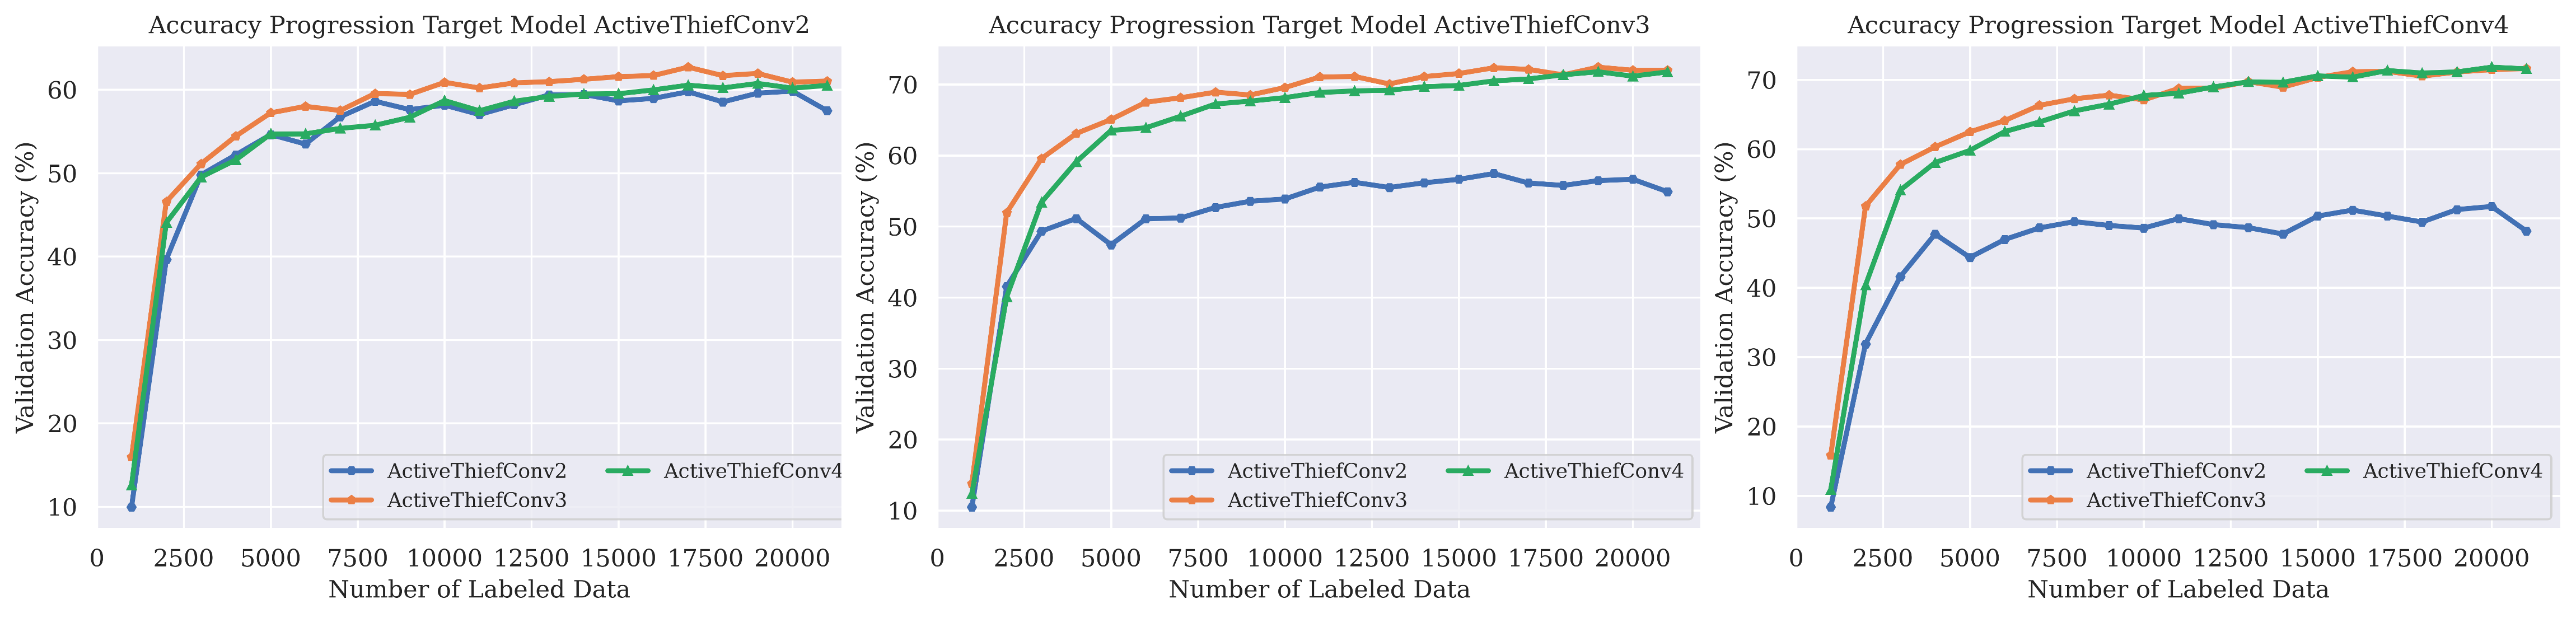
\includegraphics[width=\linewidth]{images/results_CALMS/cifar10_model_comp.png}
    \caption[Accuracy Progression for Model Stealing on CIFAR-10 using different ActiveThief models]{TODO: Nice text here}
    \label{fig:CIFAR10modelComp}
\end{figure}

\begin{figure}[h]
    \centering
    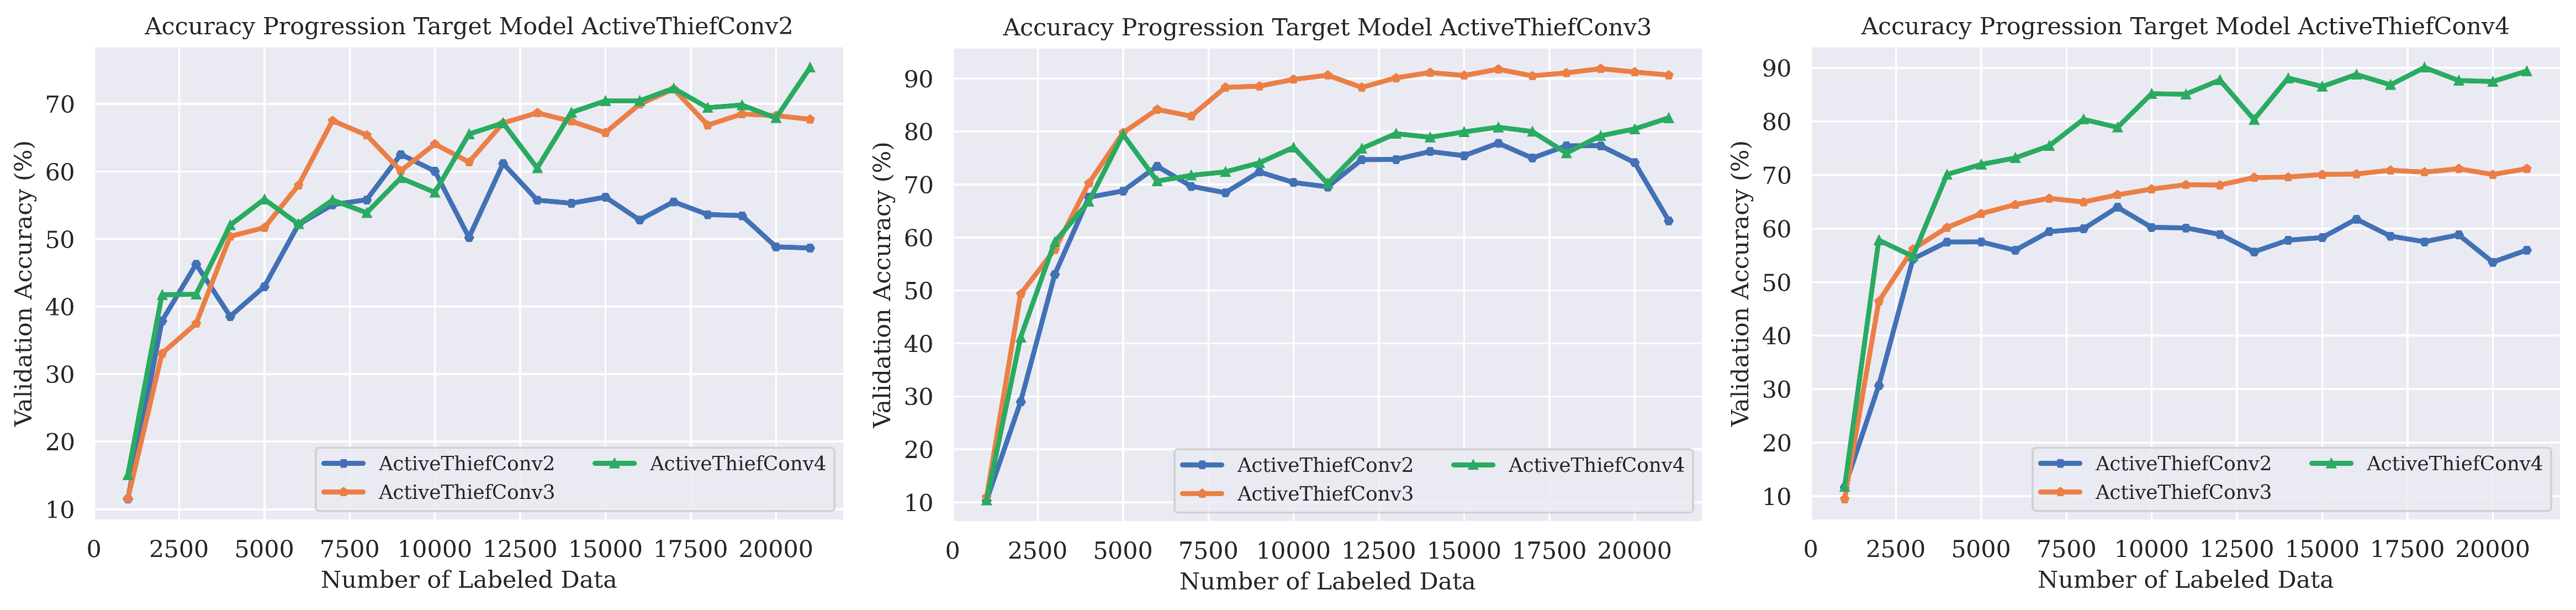
\includegraphics[width=\linewidth]{images/results_CALMS/mnist_model_comp.png}
    \caption[Accuracy Progression for Model Stealing on MNIST using different ActiveThief models]{TODO: Nice text here}
    \label{fig:MNISTmodelComp}
\end{figure}


%Tables for Cifar100
\begin{figure}[h]
    \centering
    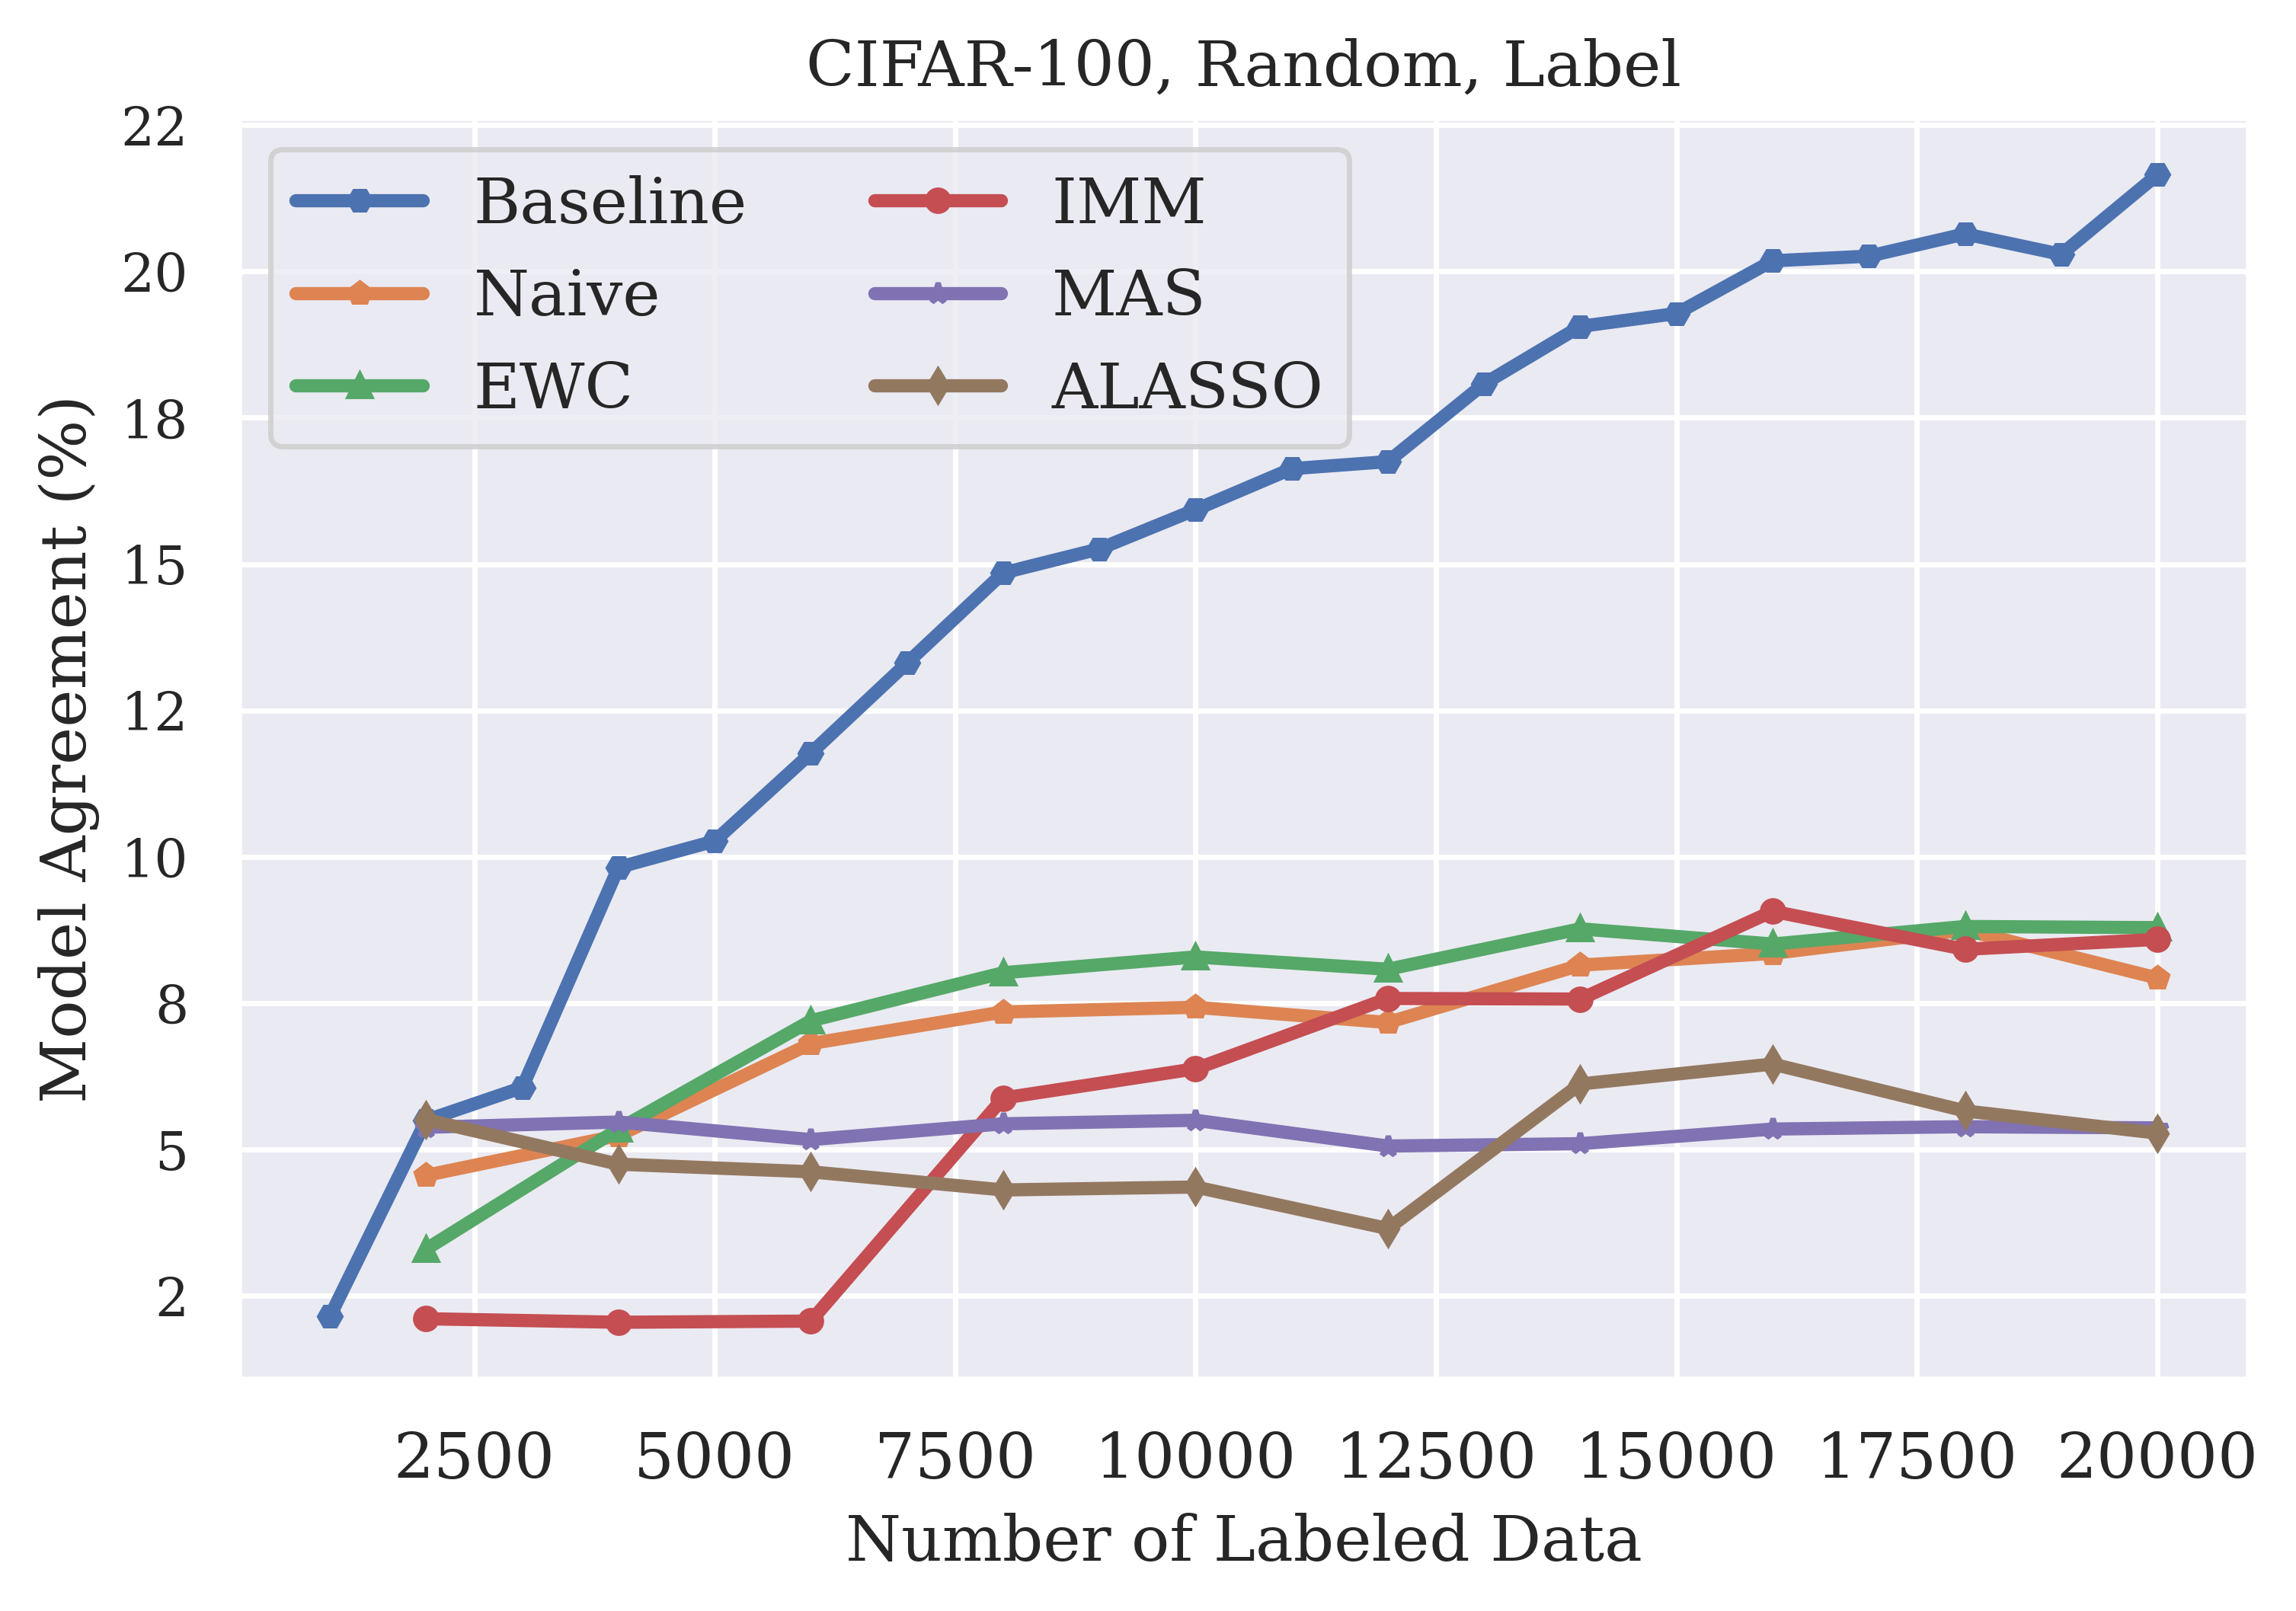
\includegraphics[width=0.8\linewidth]{images/results_CALMS/cifar100_label_random.png}
    \caption[Accuracy Comparison for Model Stealing on CIFAR100 using the top1-label and the Active Learning strategy Random]{TODO: Nice text here}
    \label{fig:CALMSCIFAR100LabelRandom}
\end{figure}

\begin{figure}[h]
    \centering
    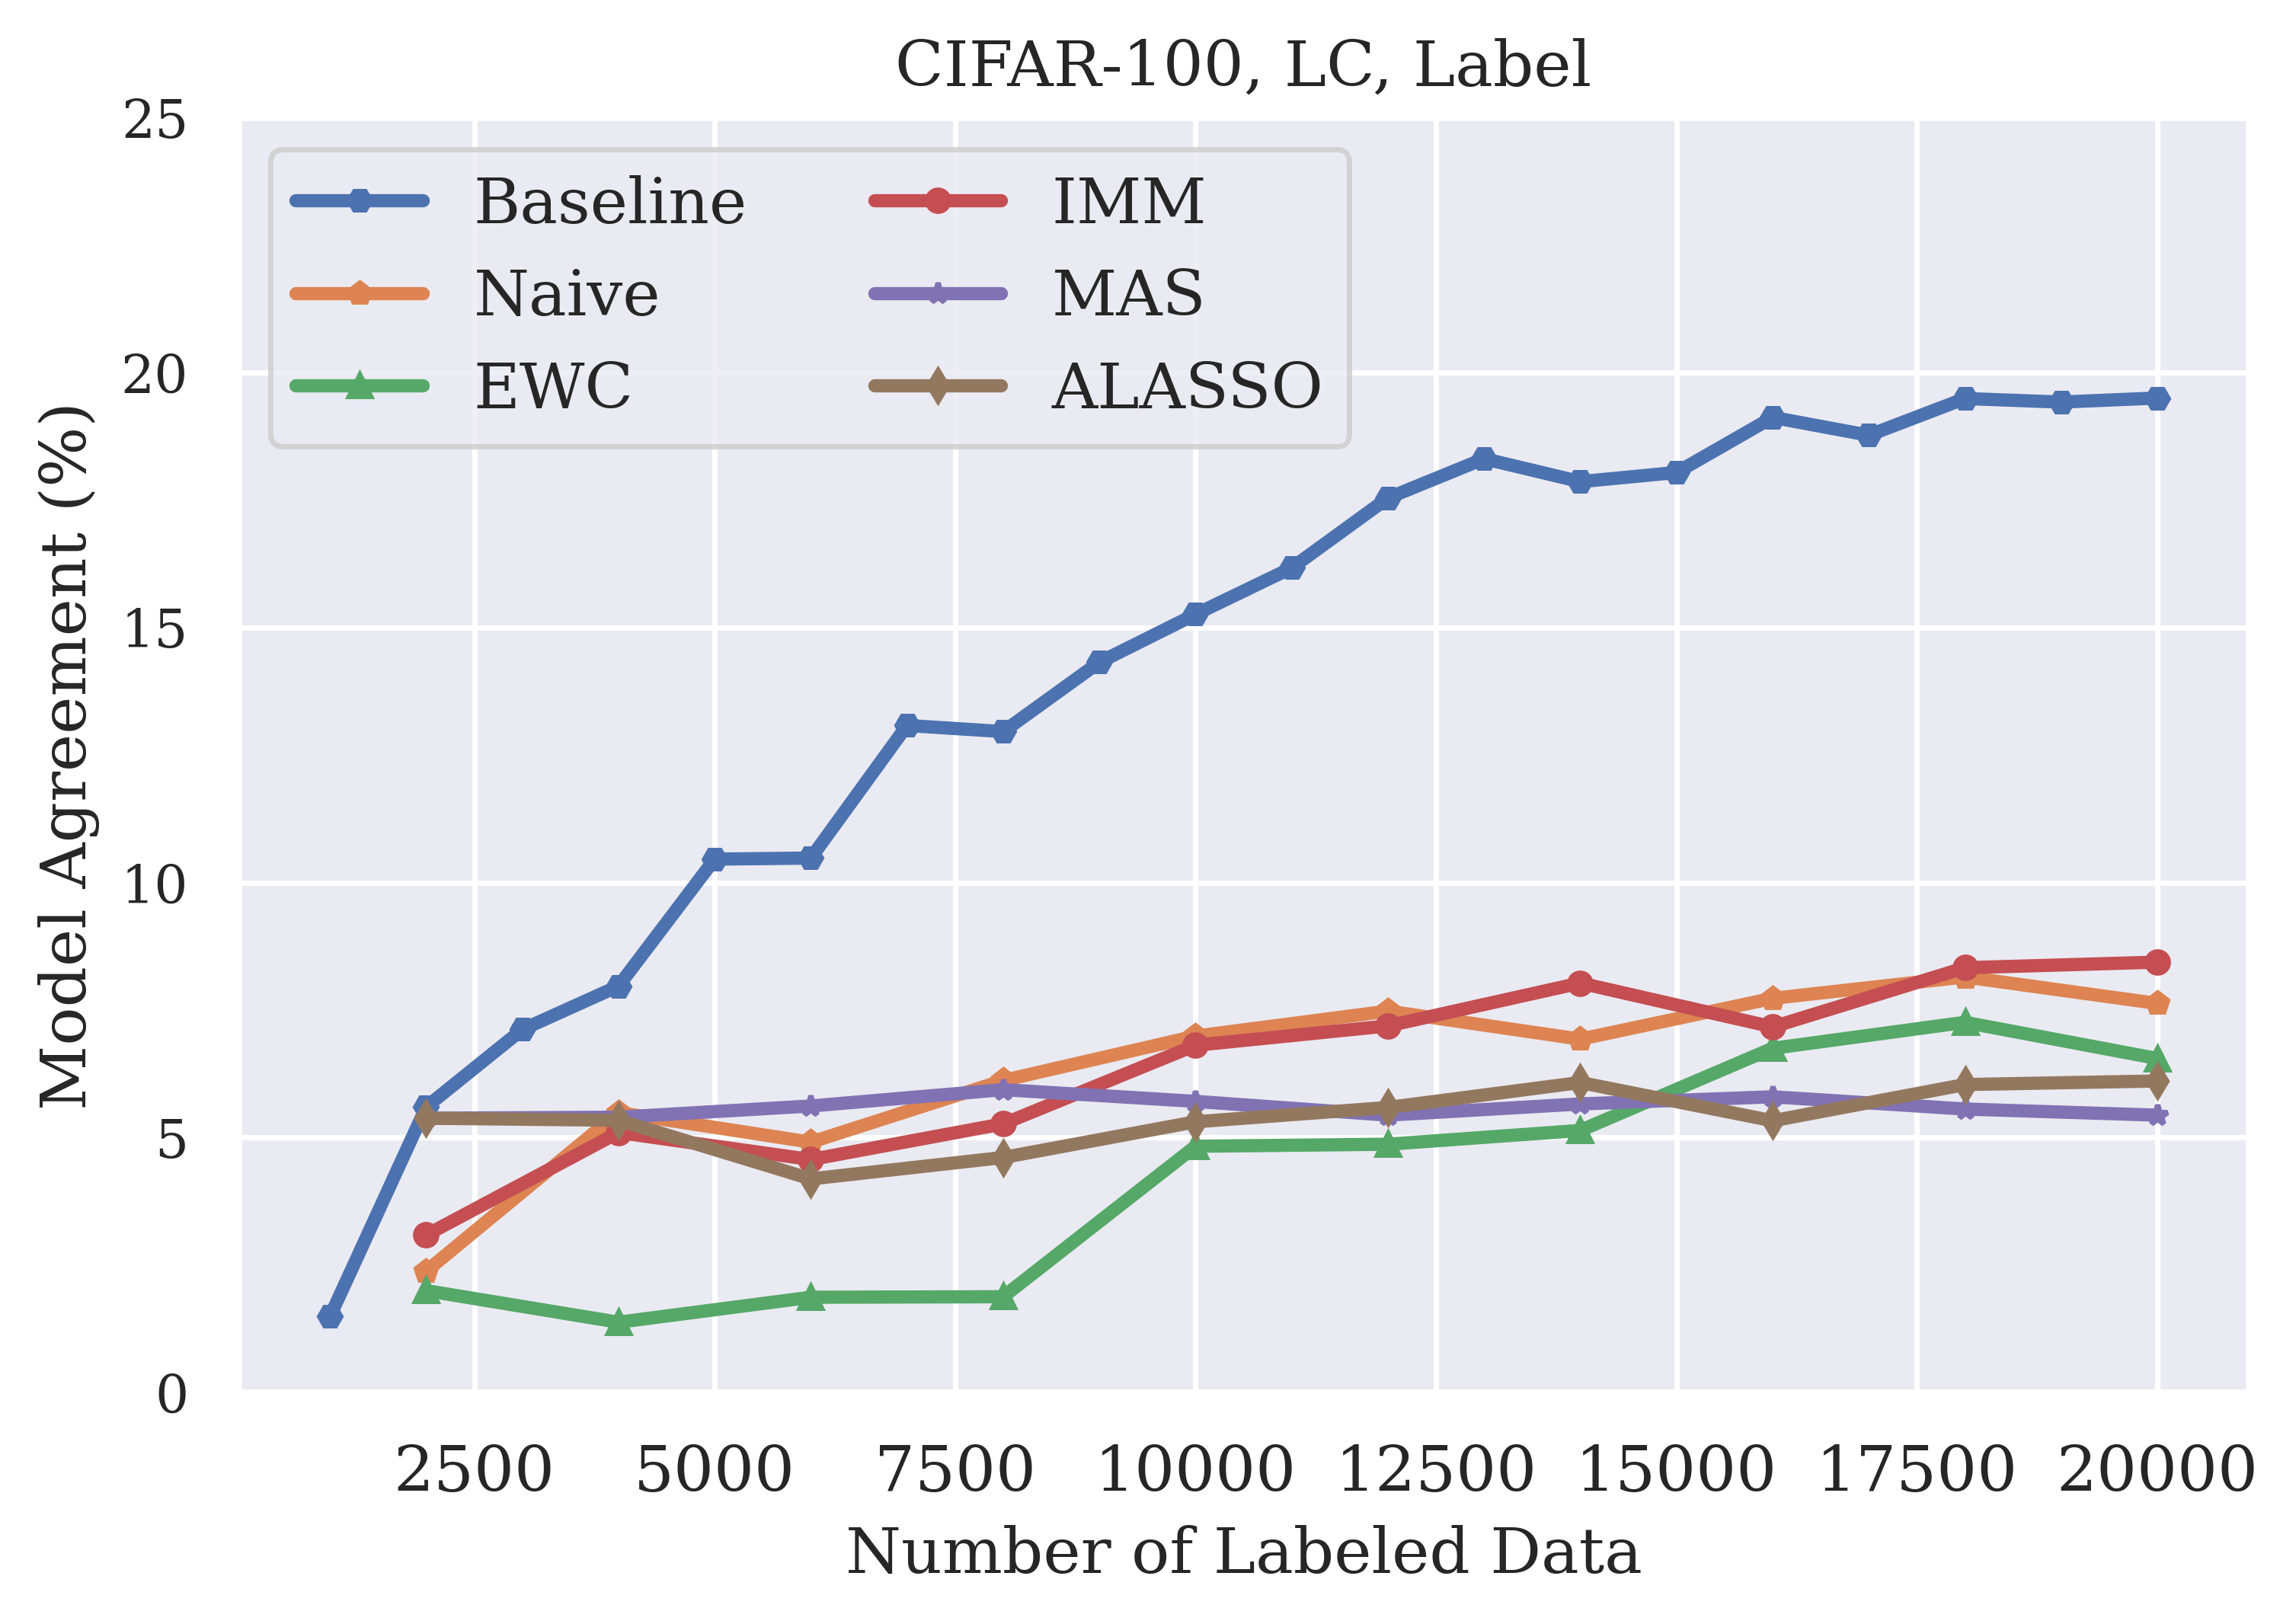
\includegraphics[width=0.8\linewidth]{images/results_CALMS/cifar100_label_lc.png}
    \caption[Accuracy Comparison for Model Stealing on CIFAR100 using the top1-label and the Active Learning strategy LC]{TODO: Nice text here}
    \label{fig:CALMSCIFAR100LabelLC}
\end{figure}

\begin{figure}[h]
    \centering
    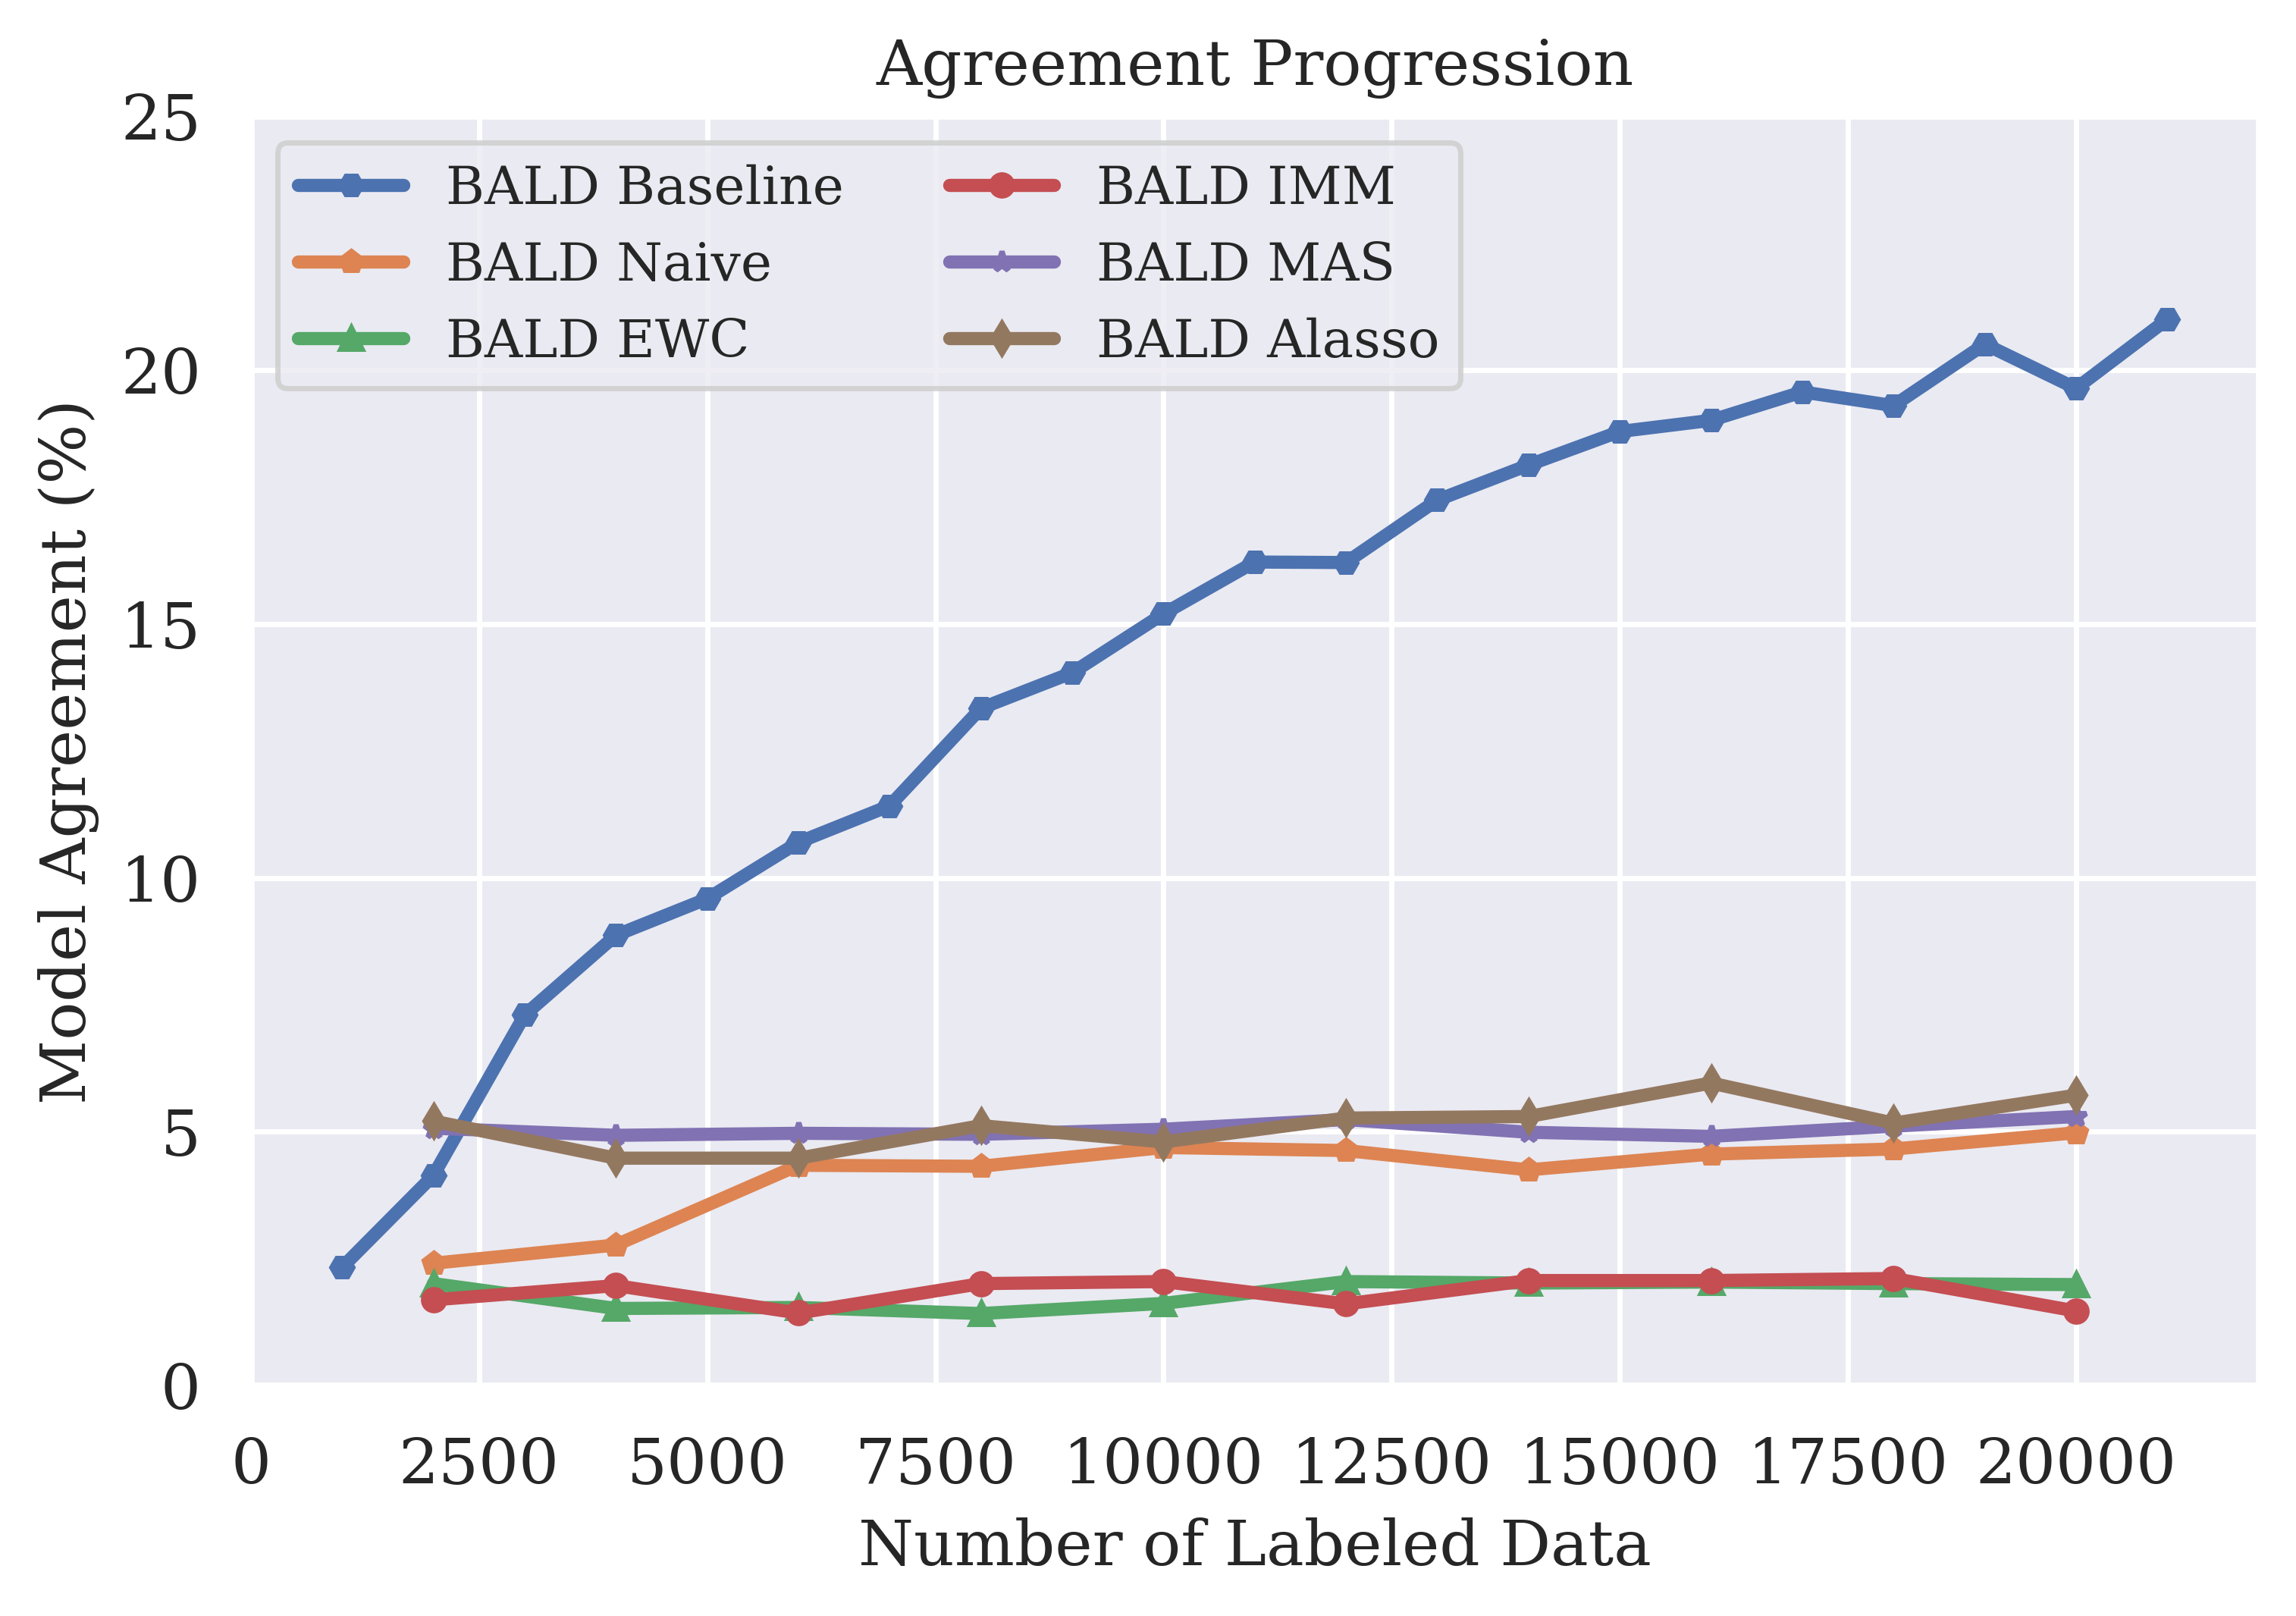
\includegraphics[width=0.8\linewidth]{images/results_CALMS/cifar100_label_bald.png}
    \caption[Accuracy Comparison for Model Stealing on CIFAR100 using the top1-label and the Active Learning strategy BALD]{TODO: Nice text here}
    \label{fig:CALMSCIFAR100LabelBALD}
\end{figure}

\begin{figure}[h]
    \centering
    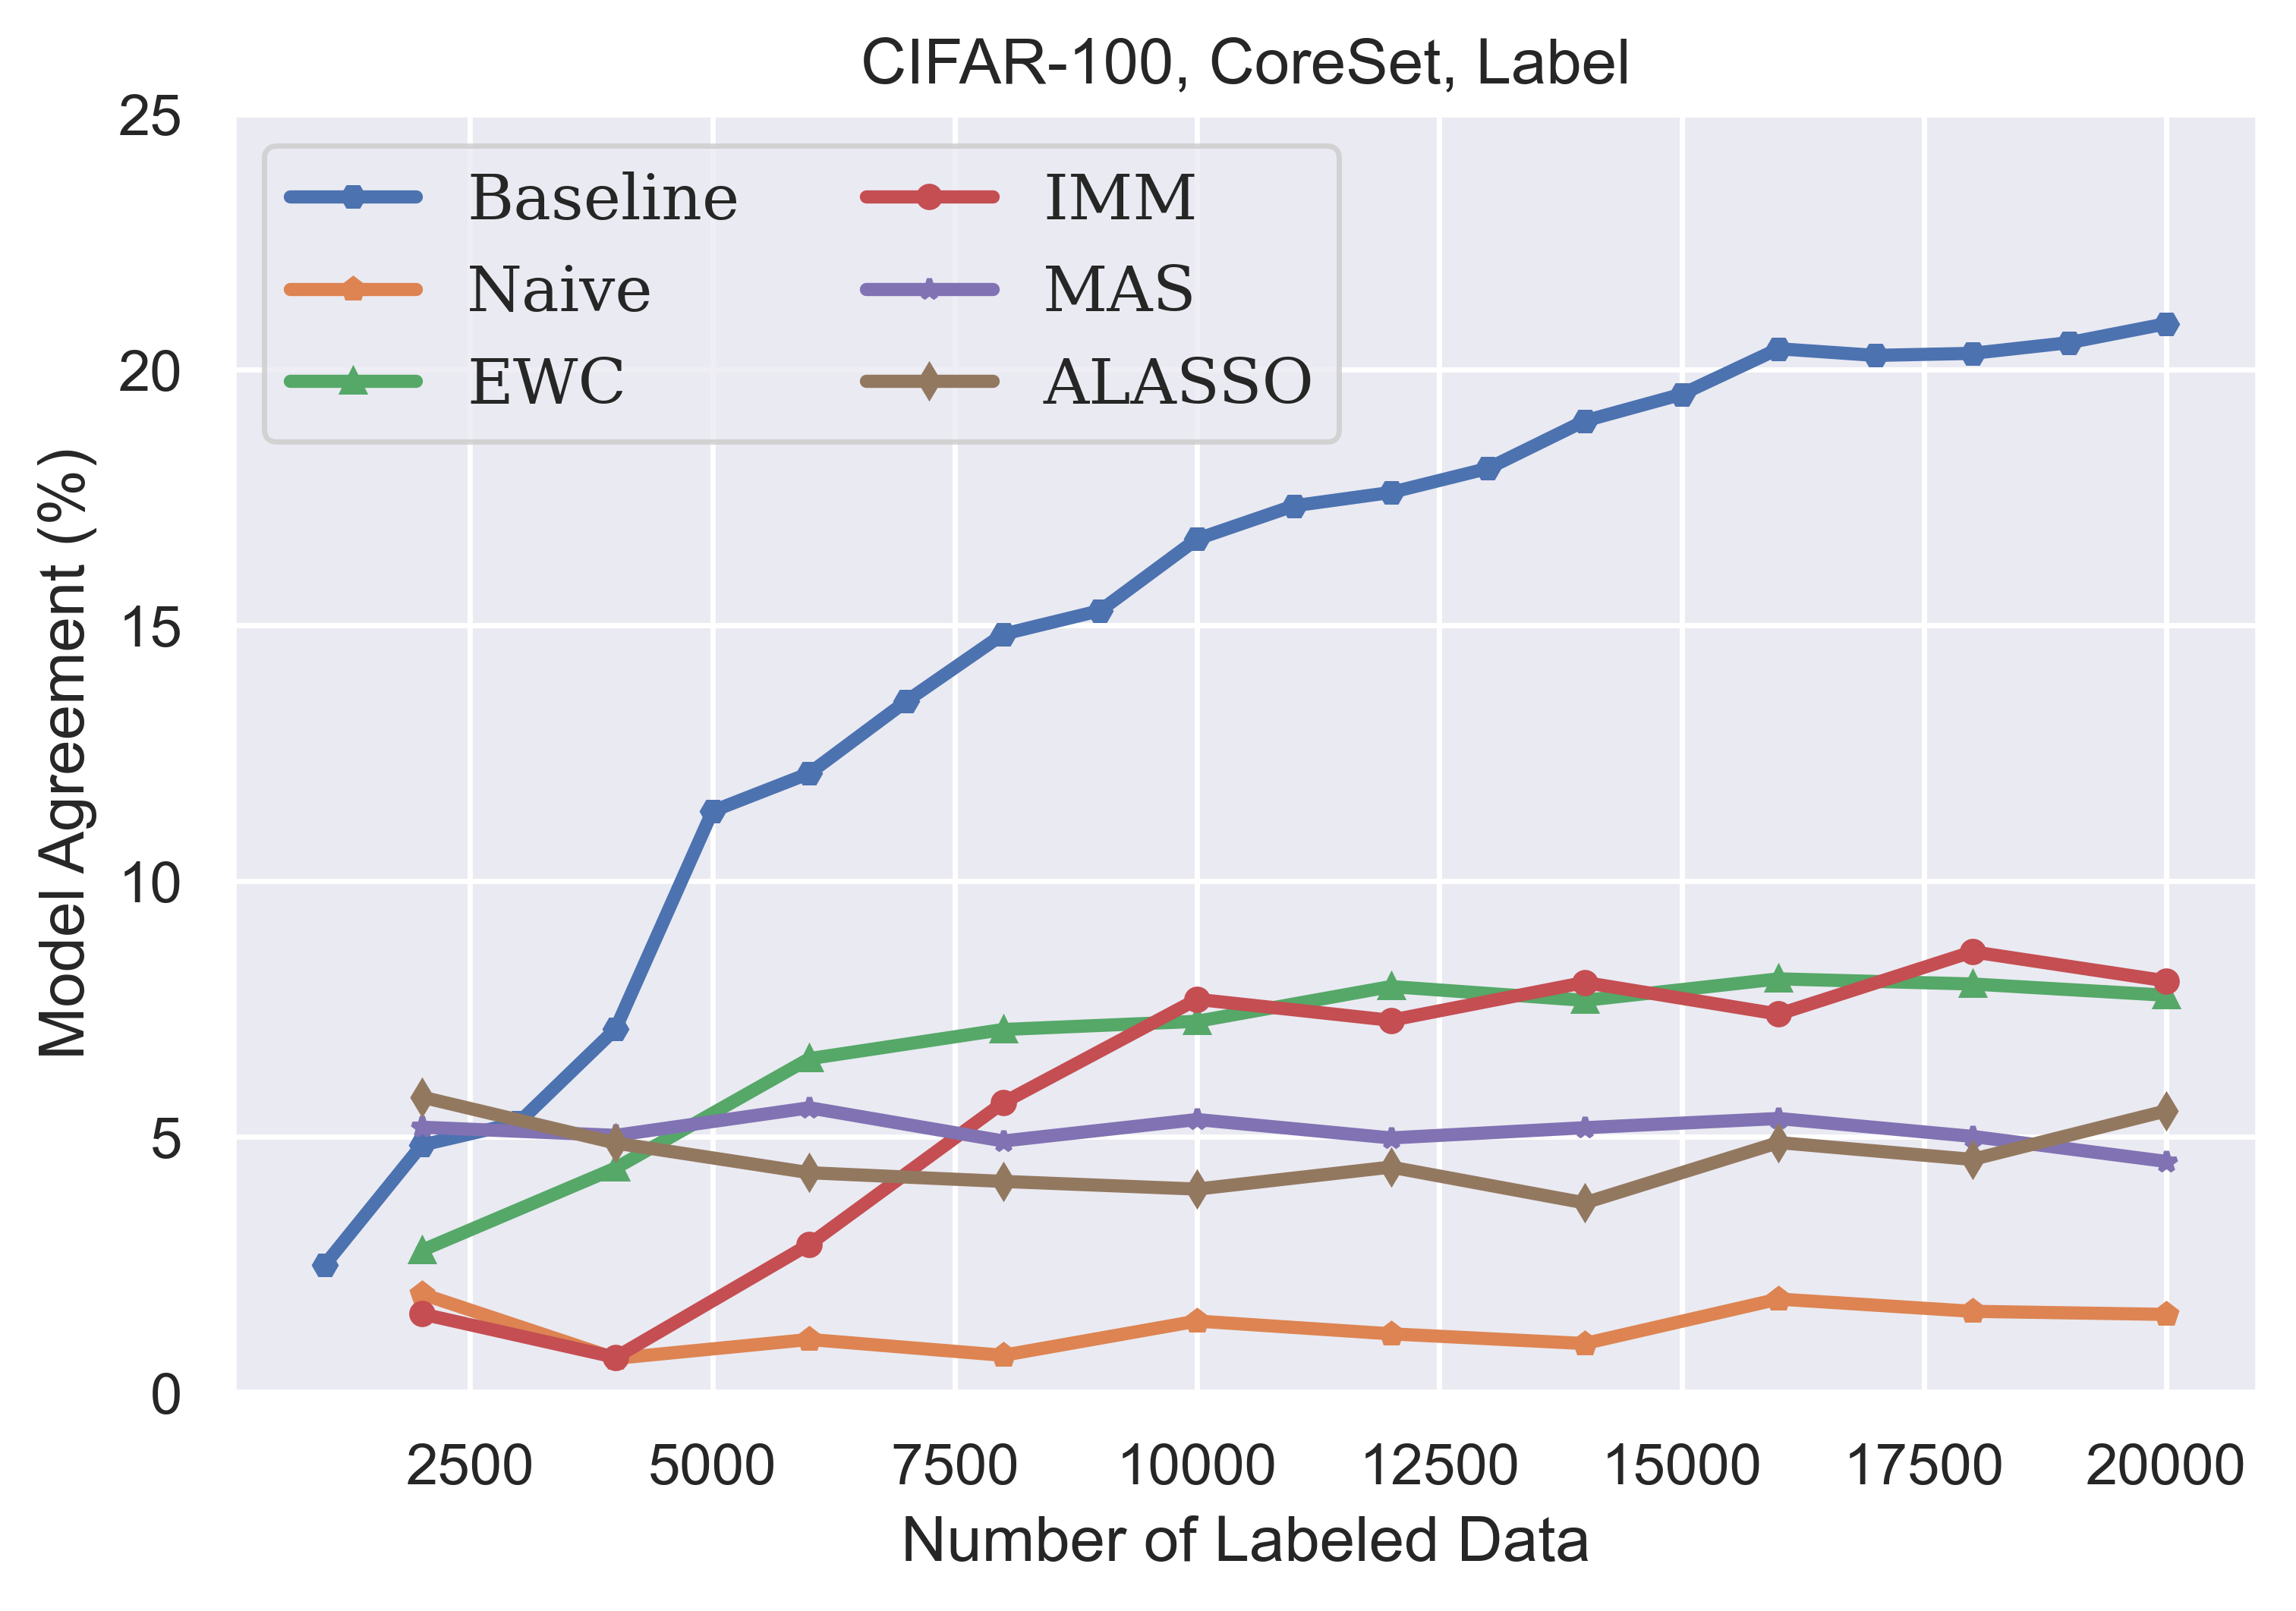
\includegraphics[width=0.8\linewidth]{images/results_CALMS/cifar100_label_coreset.png}
    \caption[Accuracy Comparison for Model Stealing on CIFAR100 using the top1-label and the Active Learning strategy CoreSet]{TODO: Nice text here}
    \label{fig:CALMSCIFAR100LabelCoreSet}
\end{figure}


\begin{figure}[h]
    \centering
    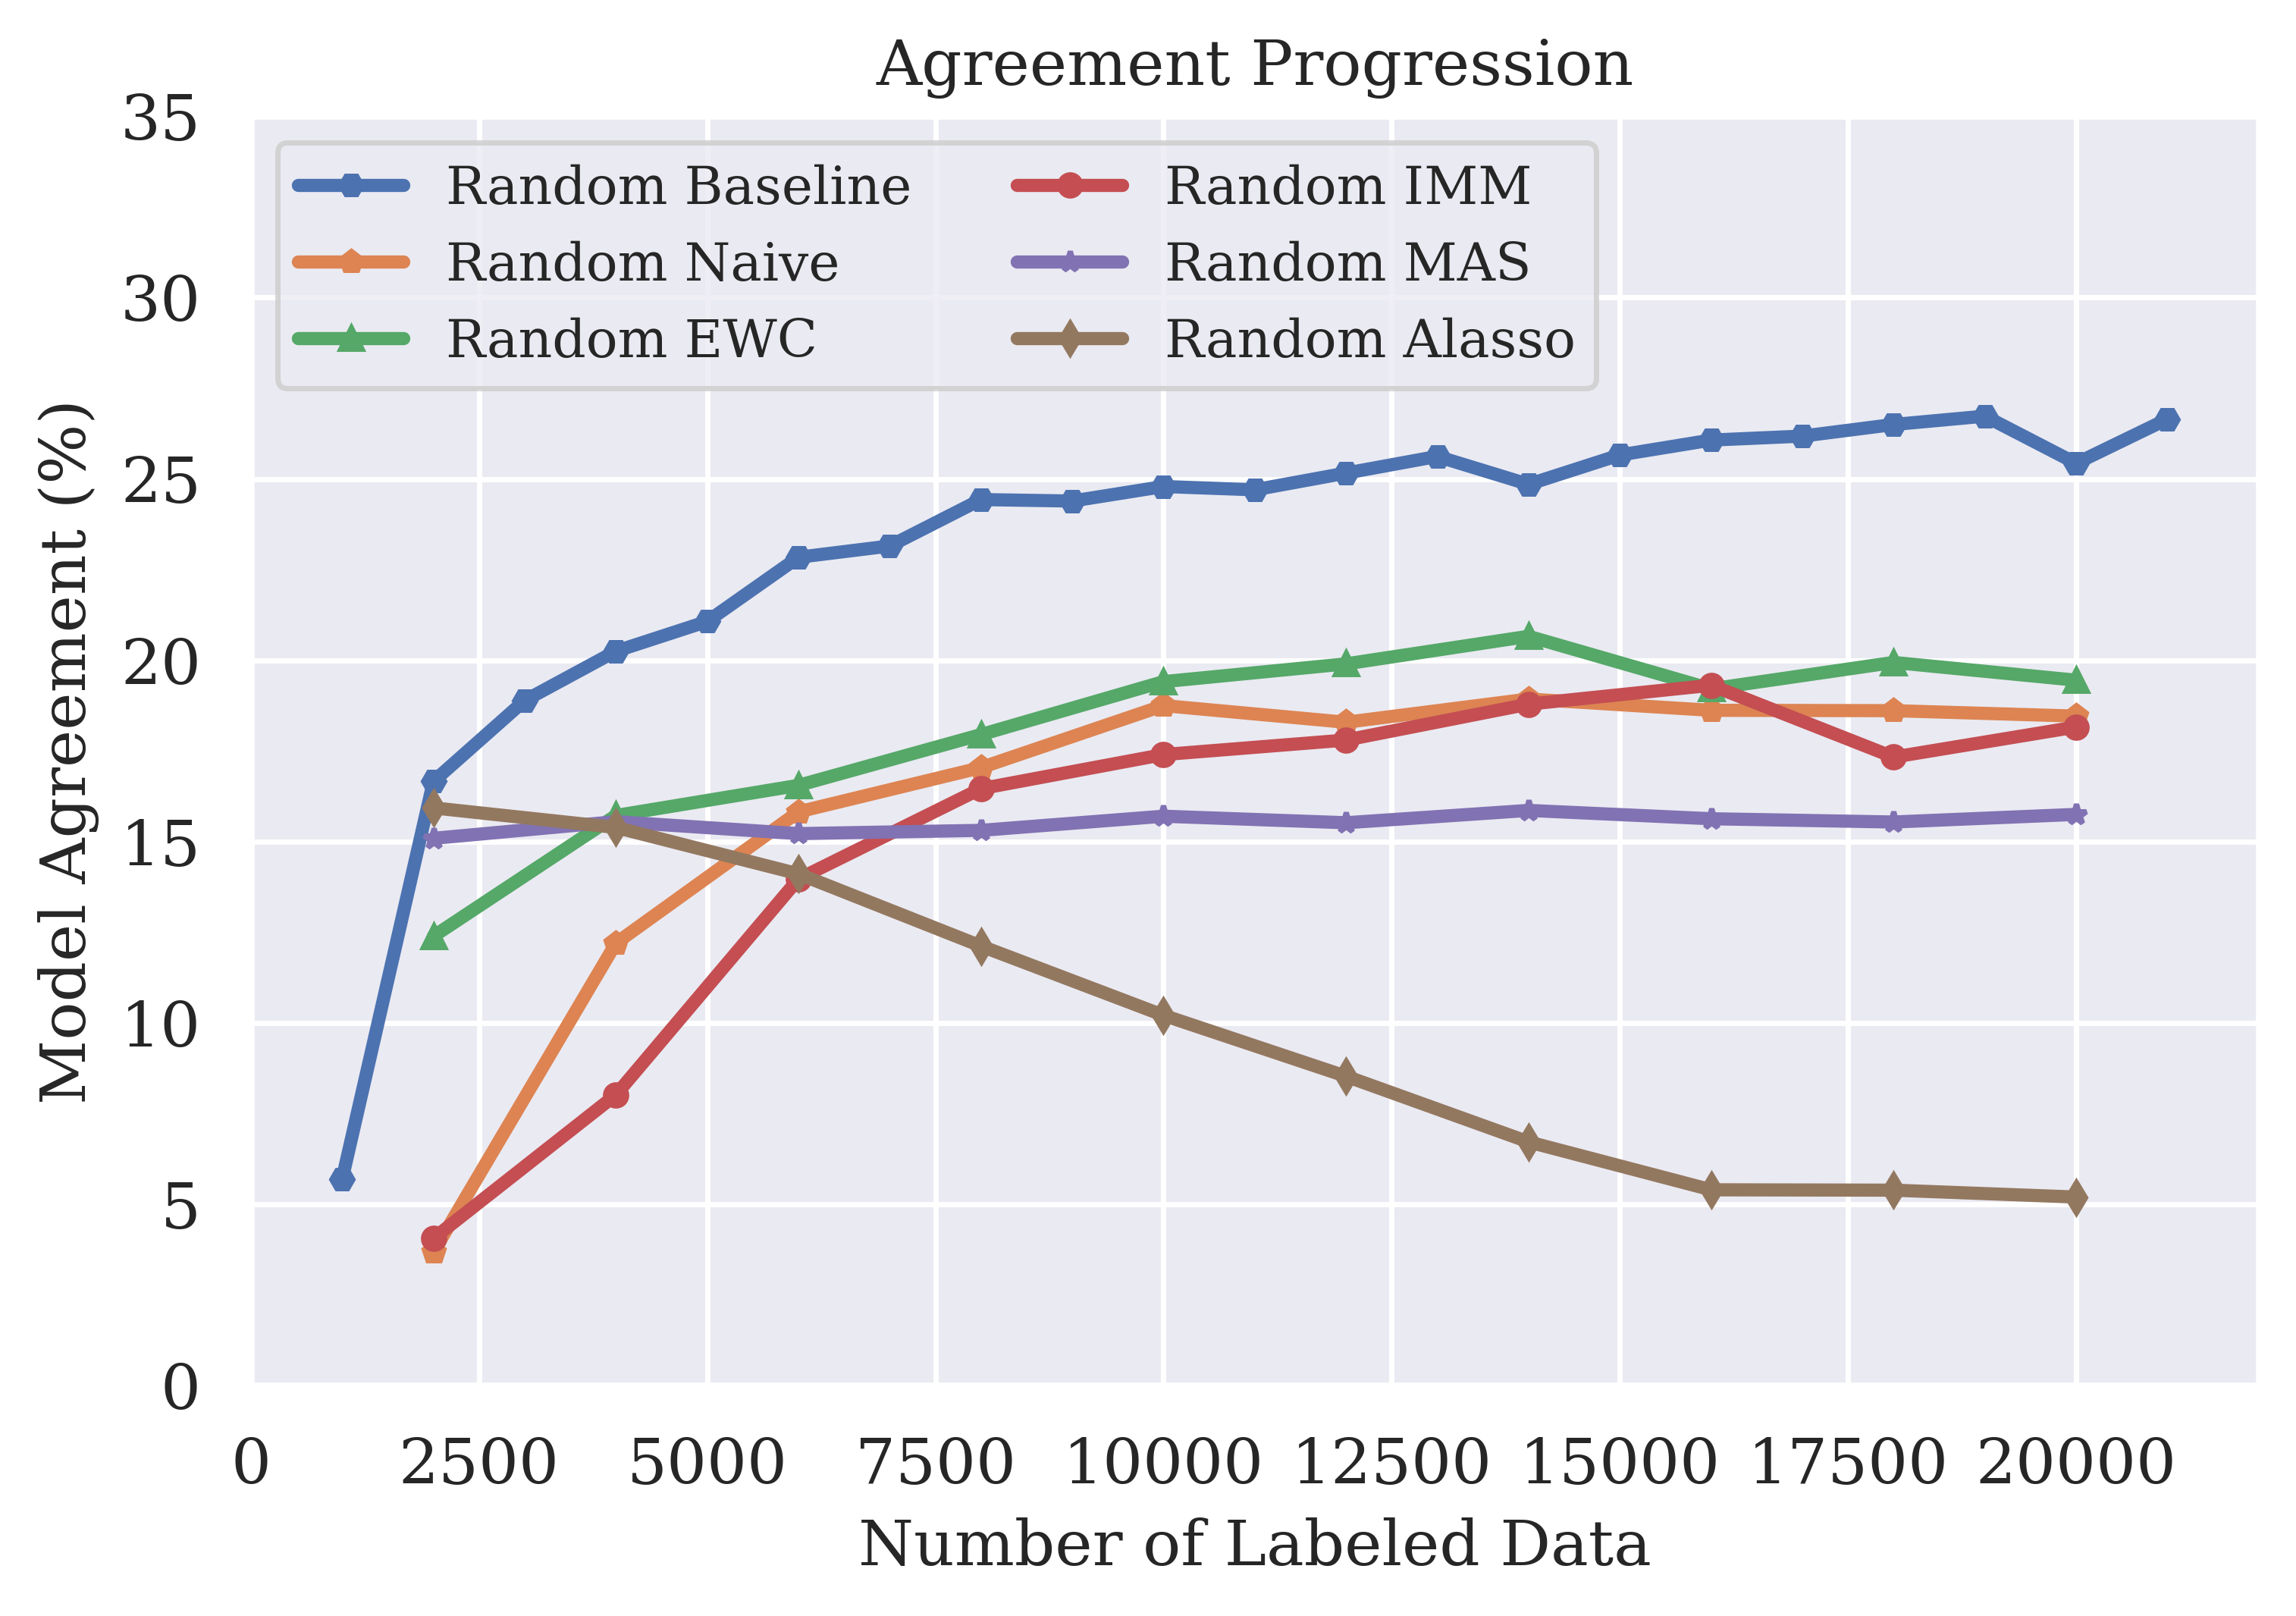
\includegraphics[width=0.8\linewidth]{images/results_CALMS/cifar100_softmax_random.png}
    \caption[Accuracy Comparison for Model Stealing on CIFAR100 using the softmax output and the Active Learning strategy Random]{TODO: Nice text here}
    \label{fig:CALMSCIFAR100SoftmaxRandom}
\end{figure}

\begin{figure}[h]
    \centering
    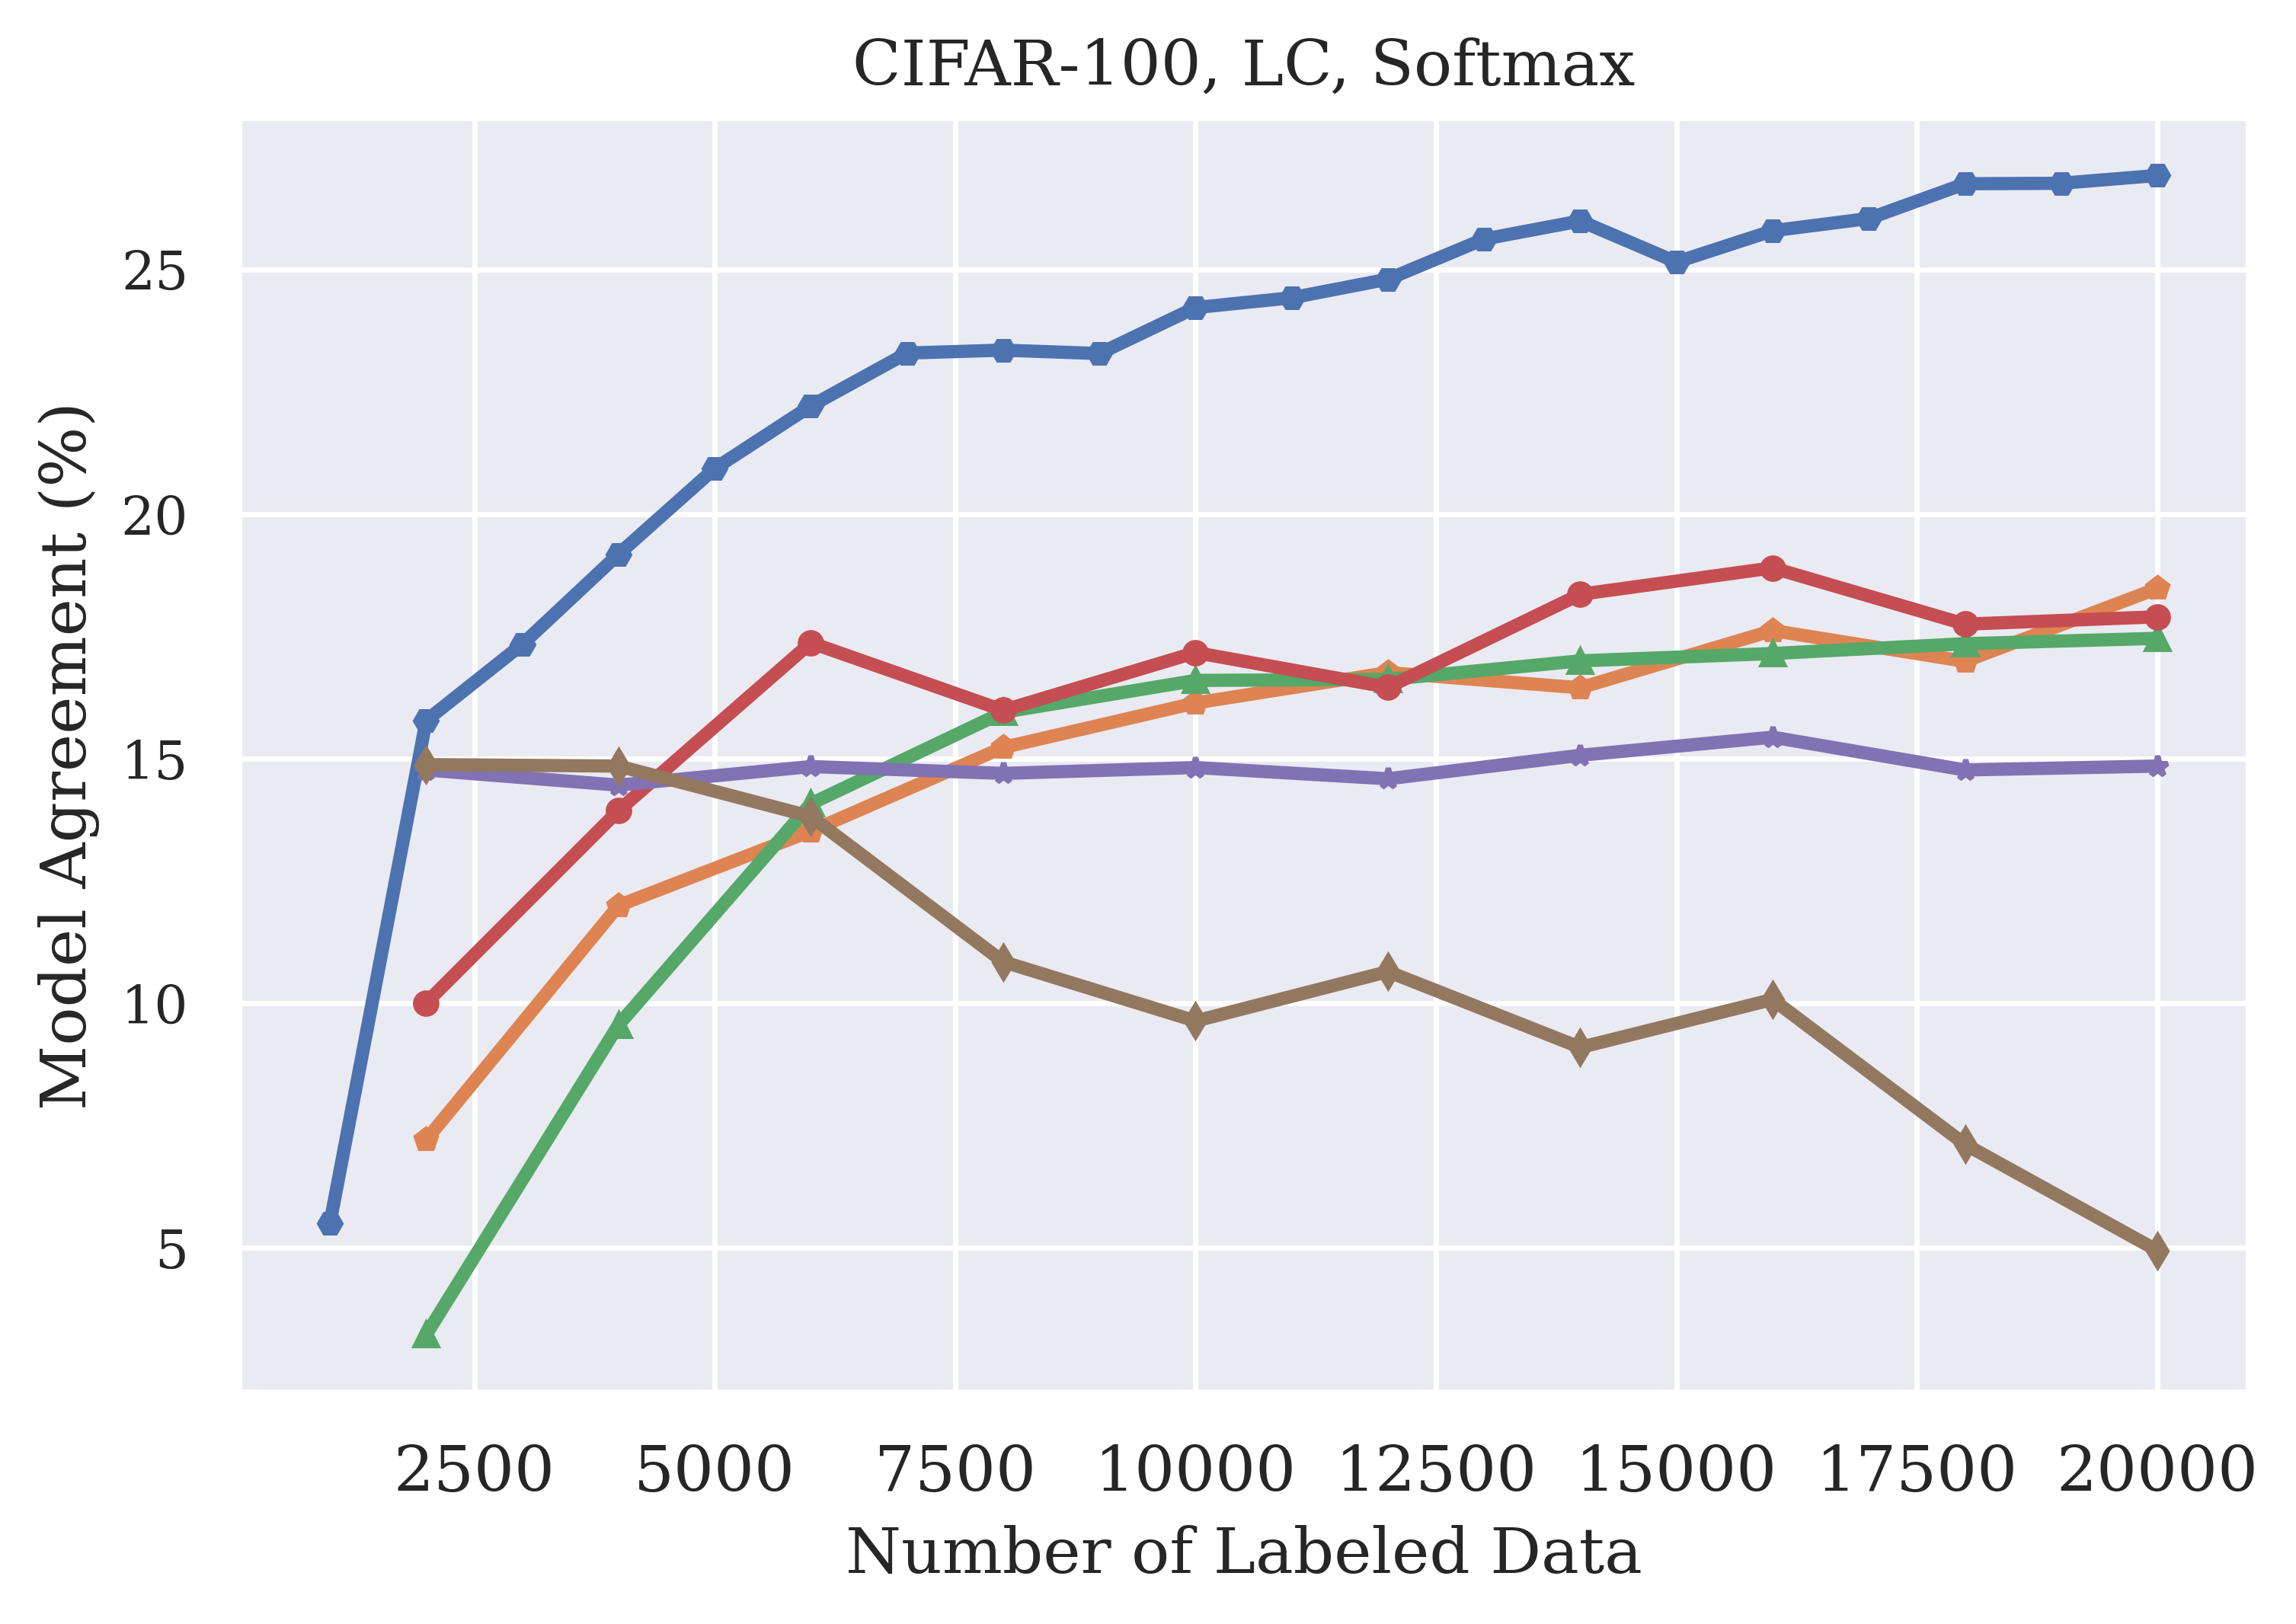
\includegraphics[width=0.8\linewidth]{images/results_CALMS/cifar100_softmax_lc.png}
    \caption[Accuracy Comparison for Model Stealing on CIFAR100 using the softmax output and the Active Learning strategy LC]{TODO: Nice text here}
    \label{fig:CALMSCIFAR100SoftmaxLC}
\end{figure}

\begin{figure}[h]
    \centering
    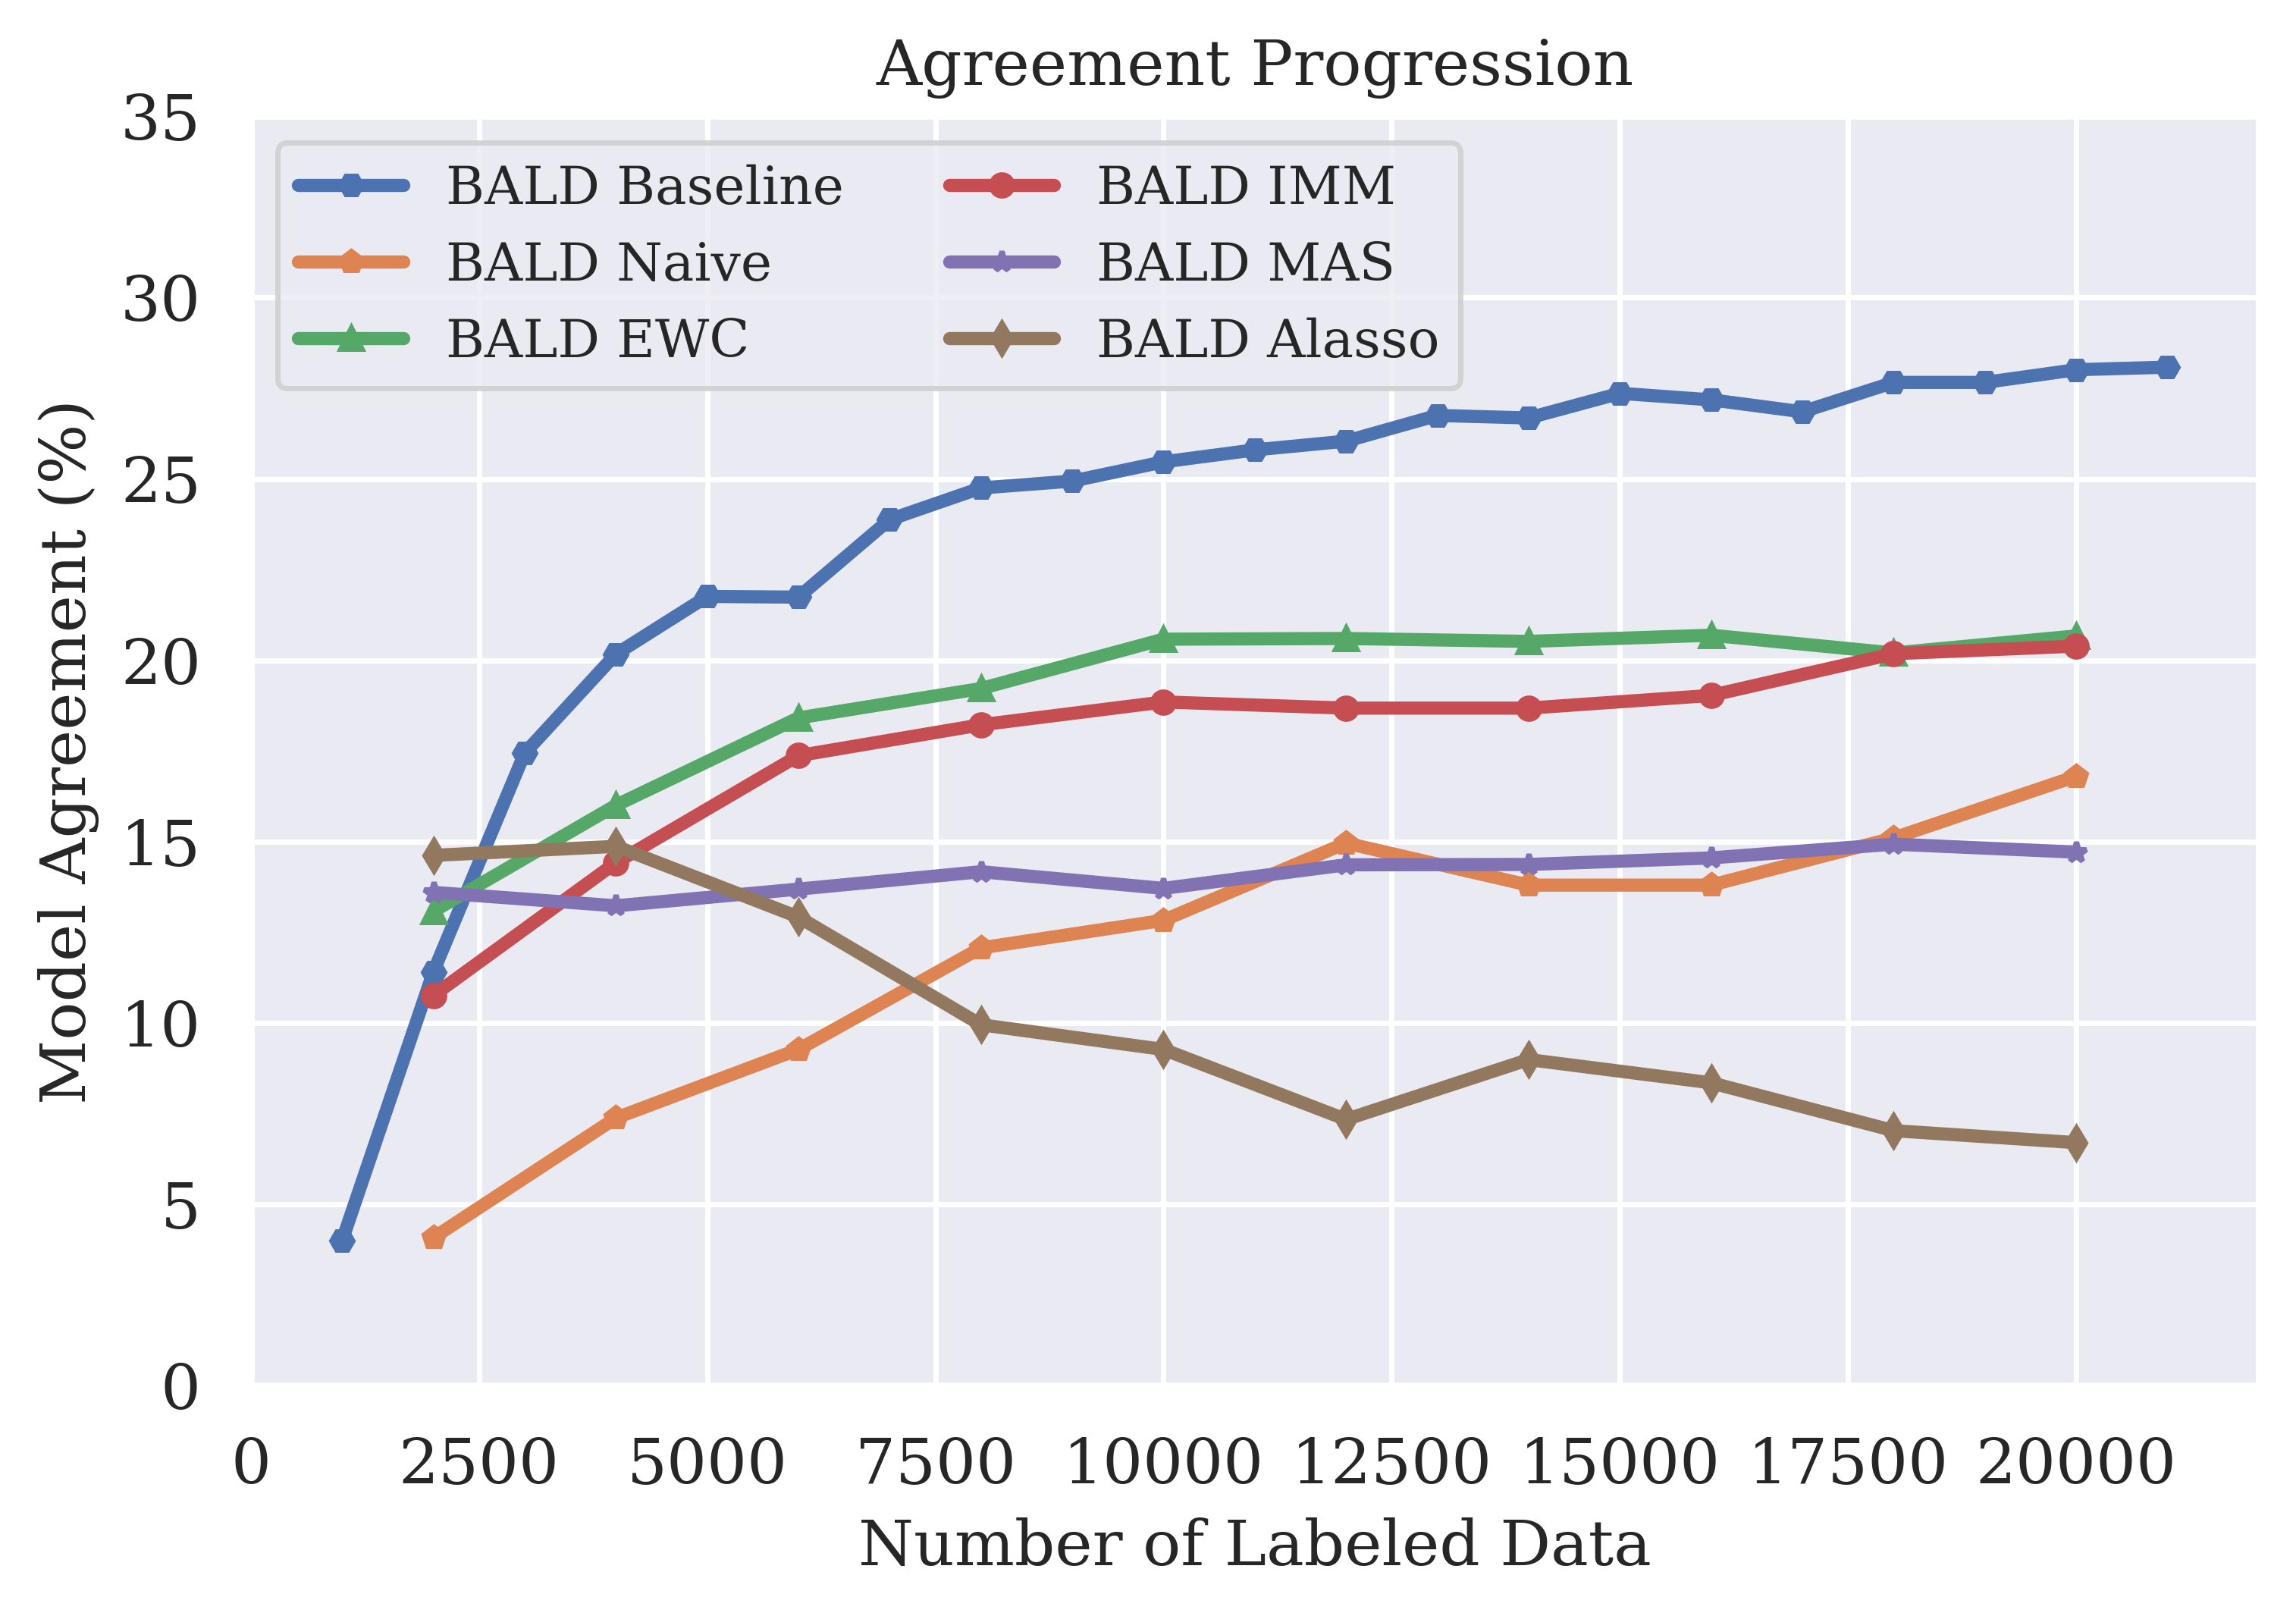
\includegraphics[width=0.8\linewidth]{images/results_CALMS/cifar100_softmax_bald.png}
    \caption[Accuracy Comparison for Model Stealing on CIFAR100 using the softmax output and the Active Learning strategy BALD]{TODO: Nice text here}
    \label{fig:CALMSCIFAR100SoftmaxBALD}
\end{figure}

\begin{figure}[h]
    \centering
    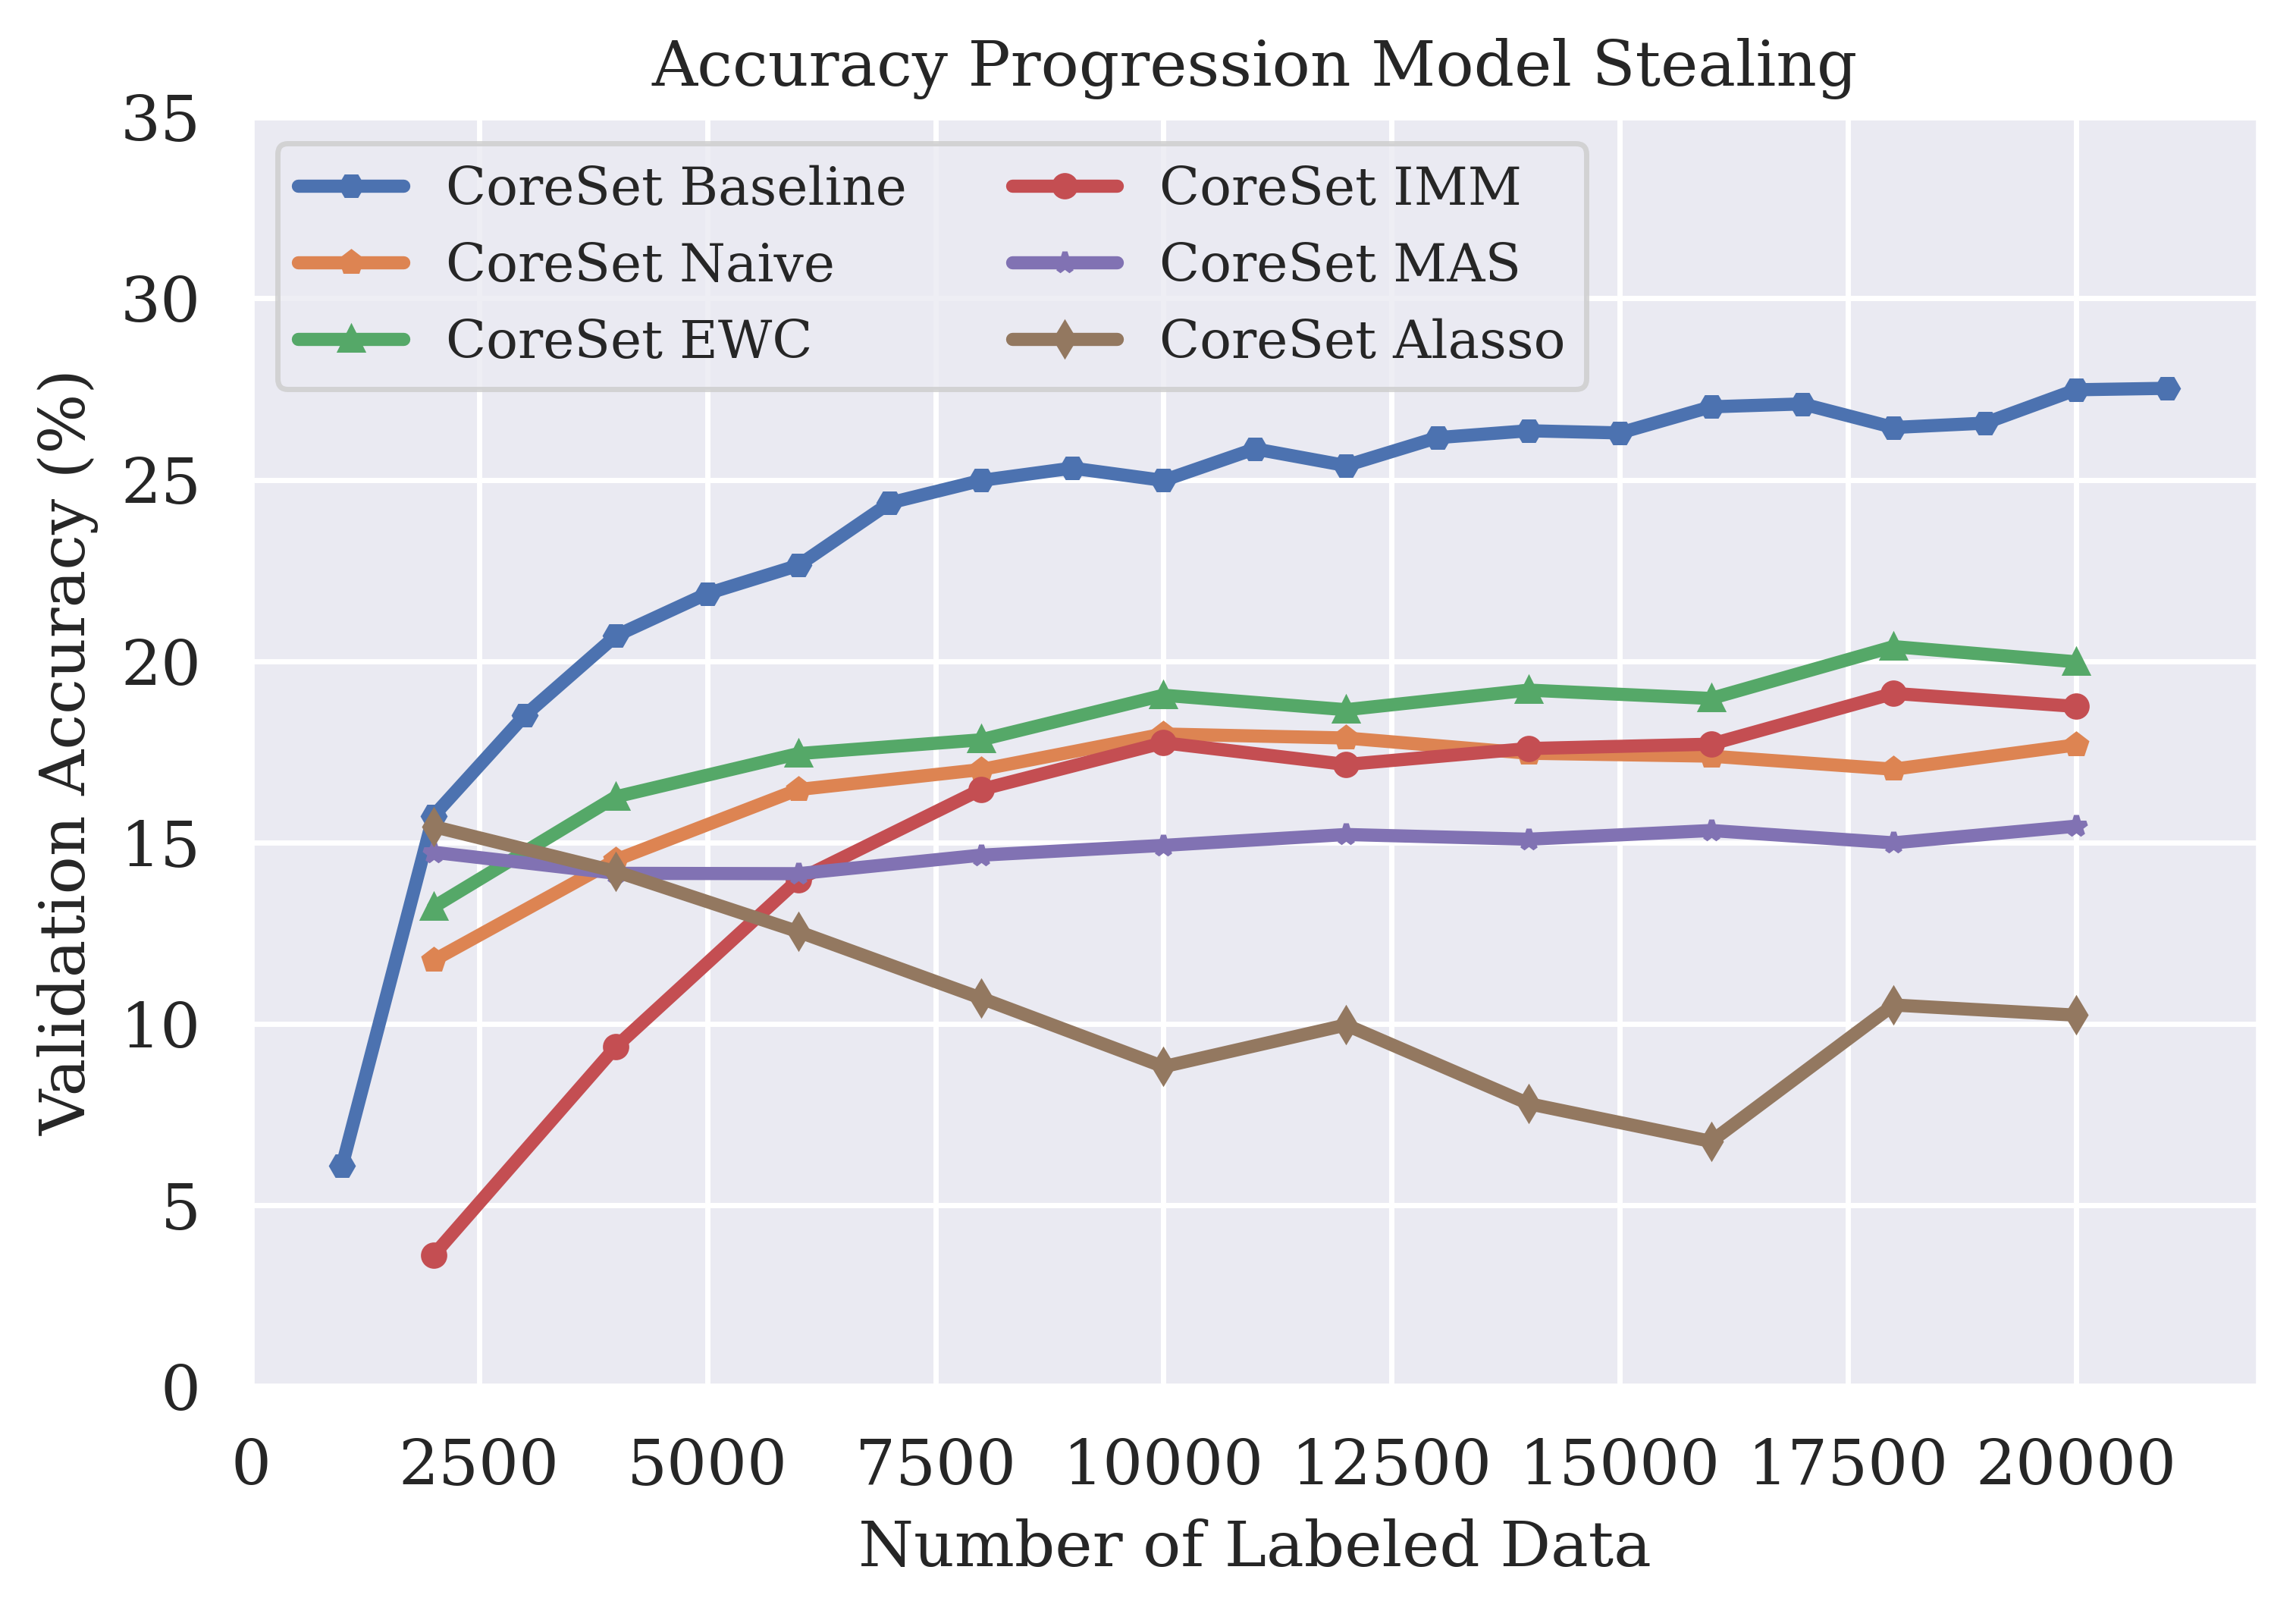
\includegraphics[width=0.8\linewidth]{images/results_CALMS/cifar100_softmax_coreset.png}
    \caption[Accuracy Comparison for Model Stealing on CIFAR100 using the softmax output and the Active Learning strategy CoreSet]{TODO: Nice text here}
    \label{fig:CALMSCIFAR100SoftmaxCoreSet}
\end{figure}

%Tables for Cifar10
%Label
\begin{figure}[h]
    \centering
    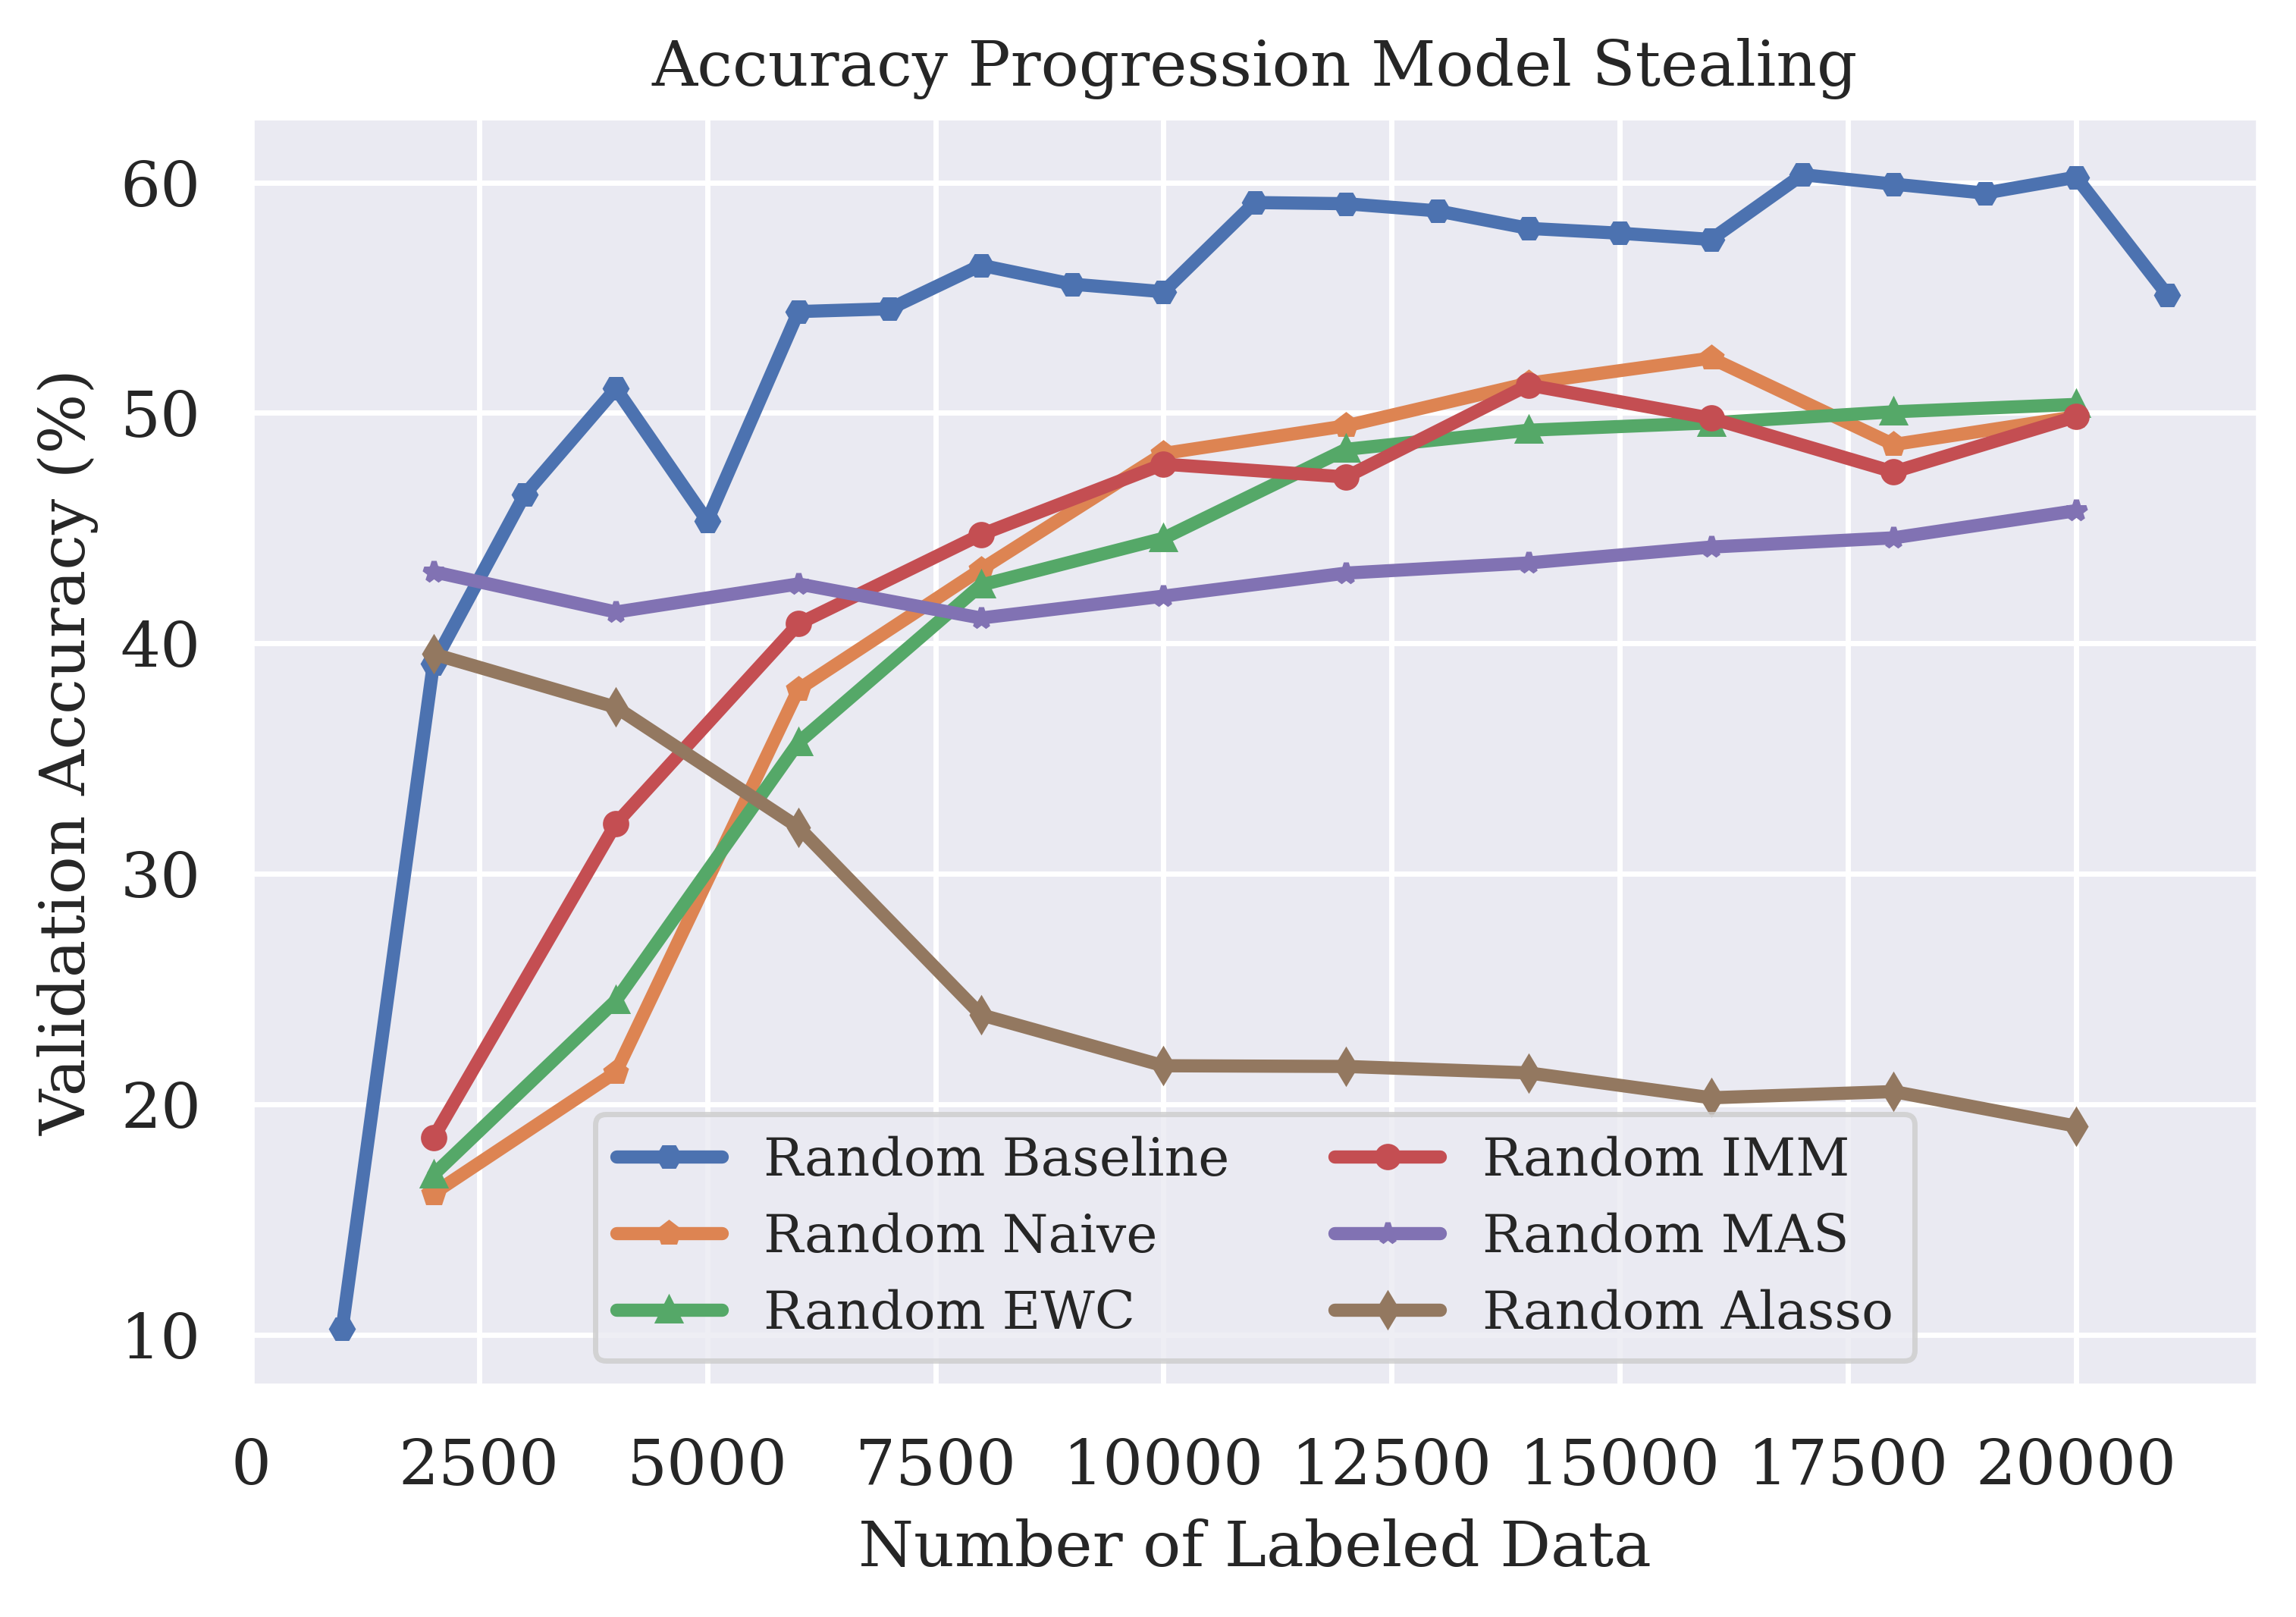
\includegraphics[width=0.8\linewidth]{images/results_CALMS/cifar_label_random.png}
    \caption[Accuracy Comparison for Model Stealing on CIFAR10 using the top1-label and the Active Learning strategy Random]{TODO: Nice text here}
    \label{fig:CALMSCIFAR10LabelRandom}
\end{figure}

\begin{figure}[h]
    \centering
    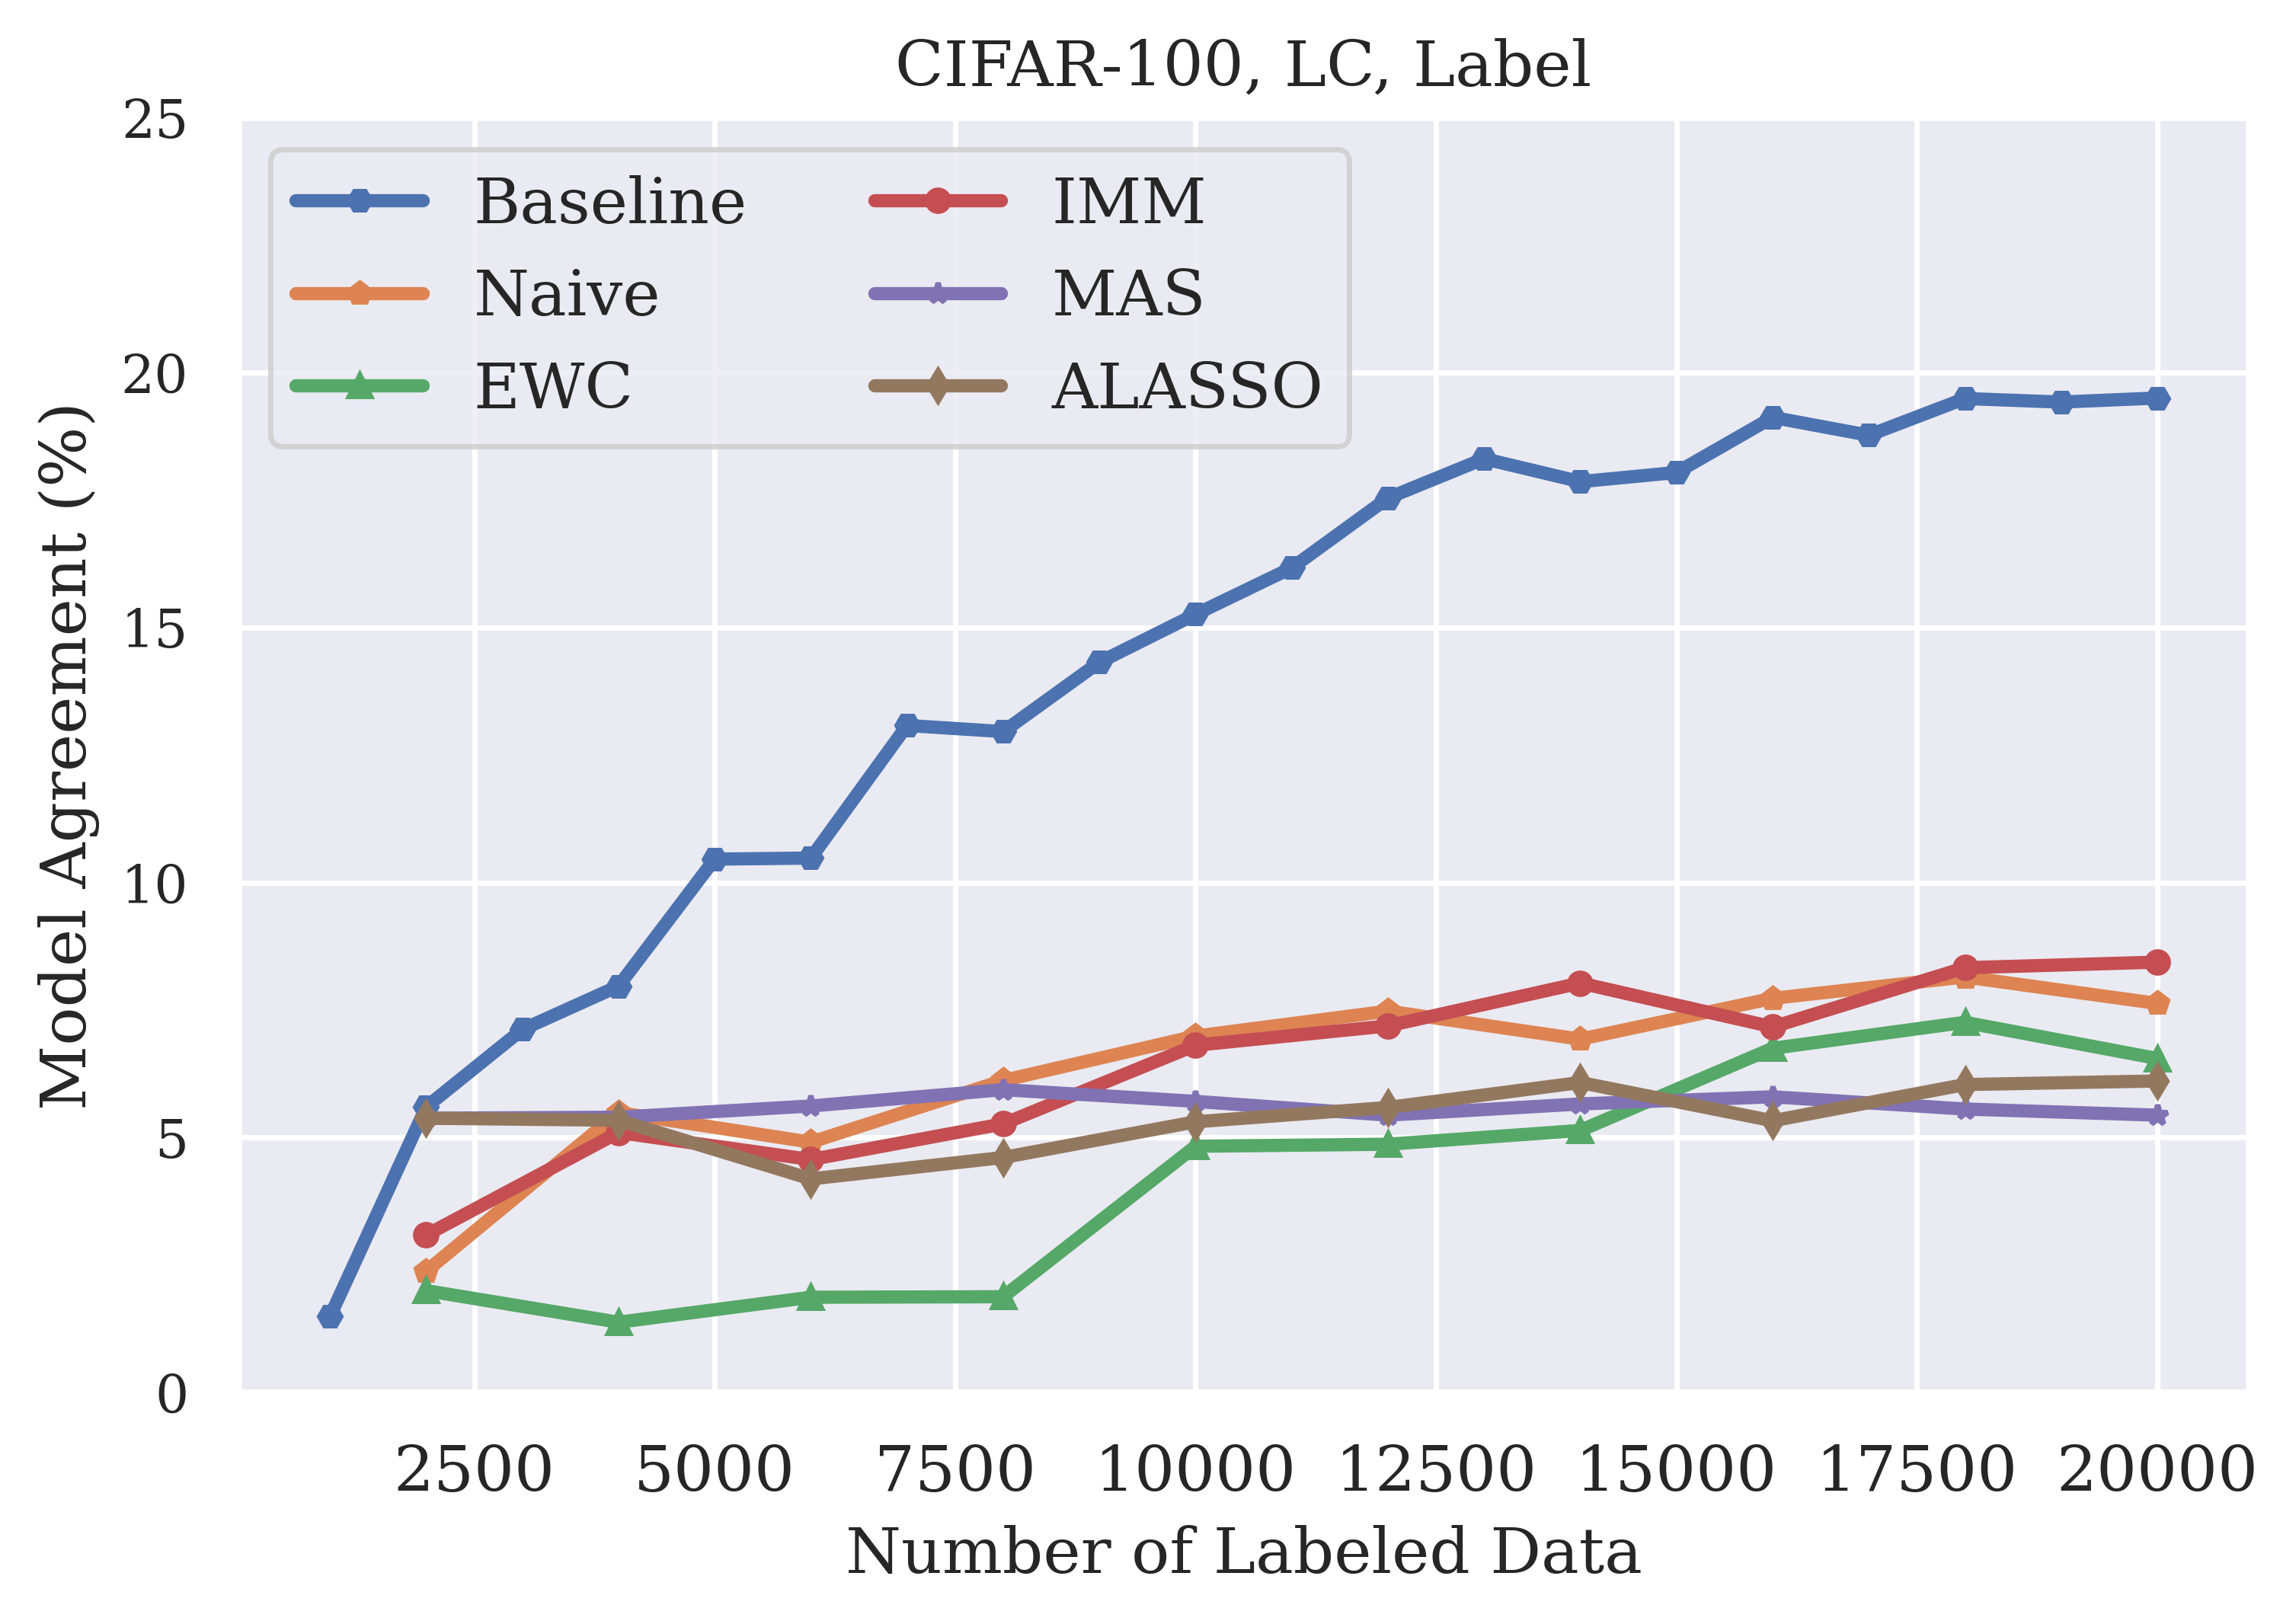
\includegraphics[width=0.8\linewidth]{images/results_CALMS/cifar100_label_lc.png}
    \caption[Accuracy Comparison for Model Stealing on CIFAR10 using the top1-label and the Active Learning strategy LC]{TODO: Nice text here}
    \label{fig:CALMSCIFAR10LabelLC}
\end{figure}

\begin{figure}[h]
    \centering
    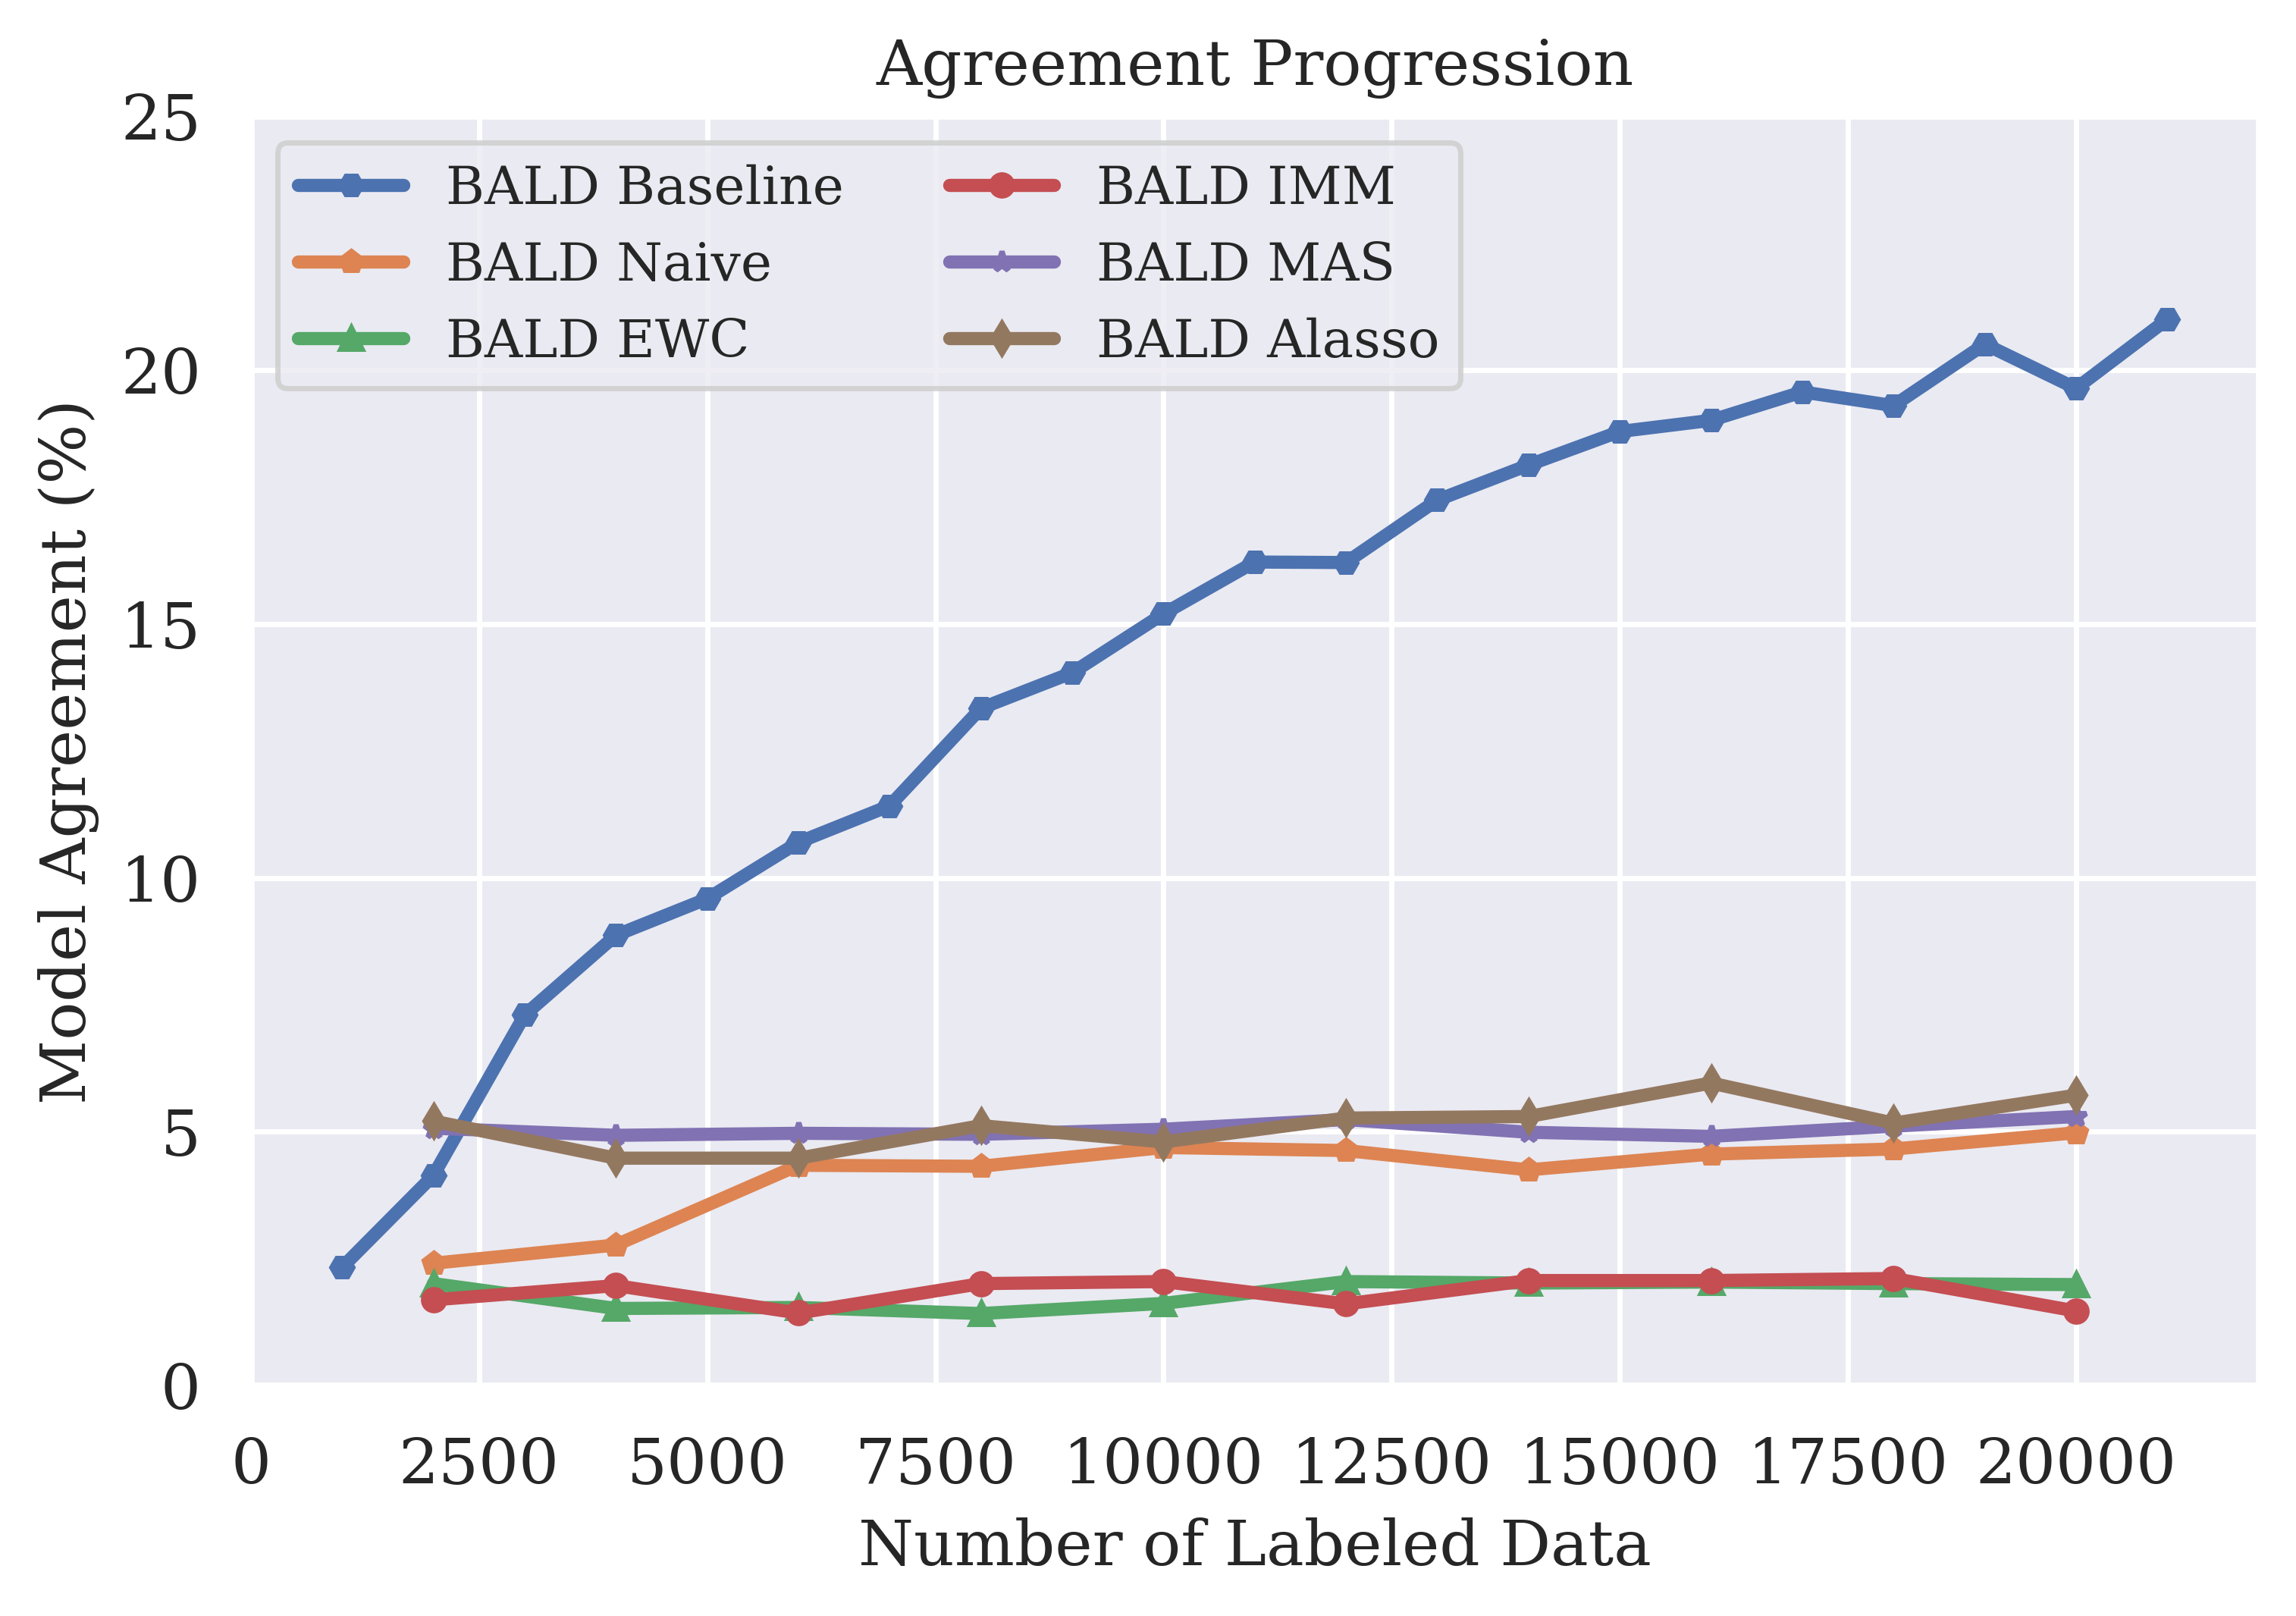
\includegraphics[width=0.8\linewidth]{images/results_CALMS/cifar100_label_bald.png}
    \caption[Accuracy Comparison for Model Stealing on CIFAR10 using the top1-label and the Active Learning strategy BALD]{TODO: Nice text here}
    \label{fig:CALMSCIFAR10LabelBALD}
\end{figure}

\begin{figure}[h]
    \centering
    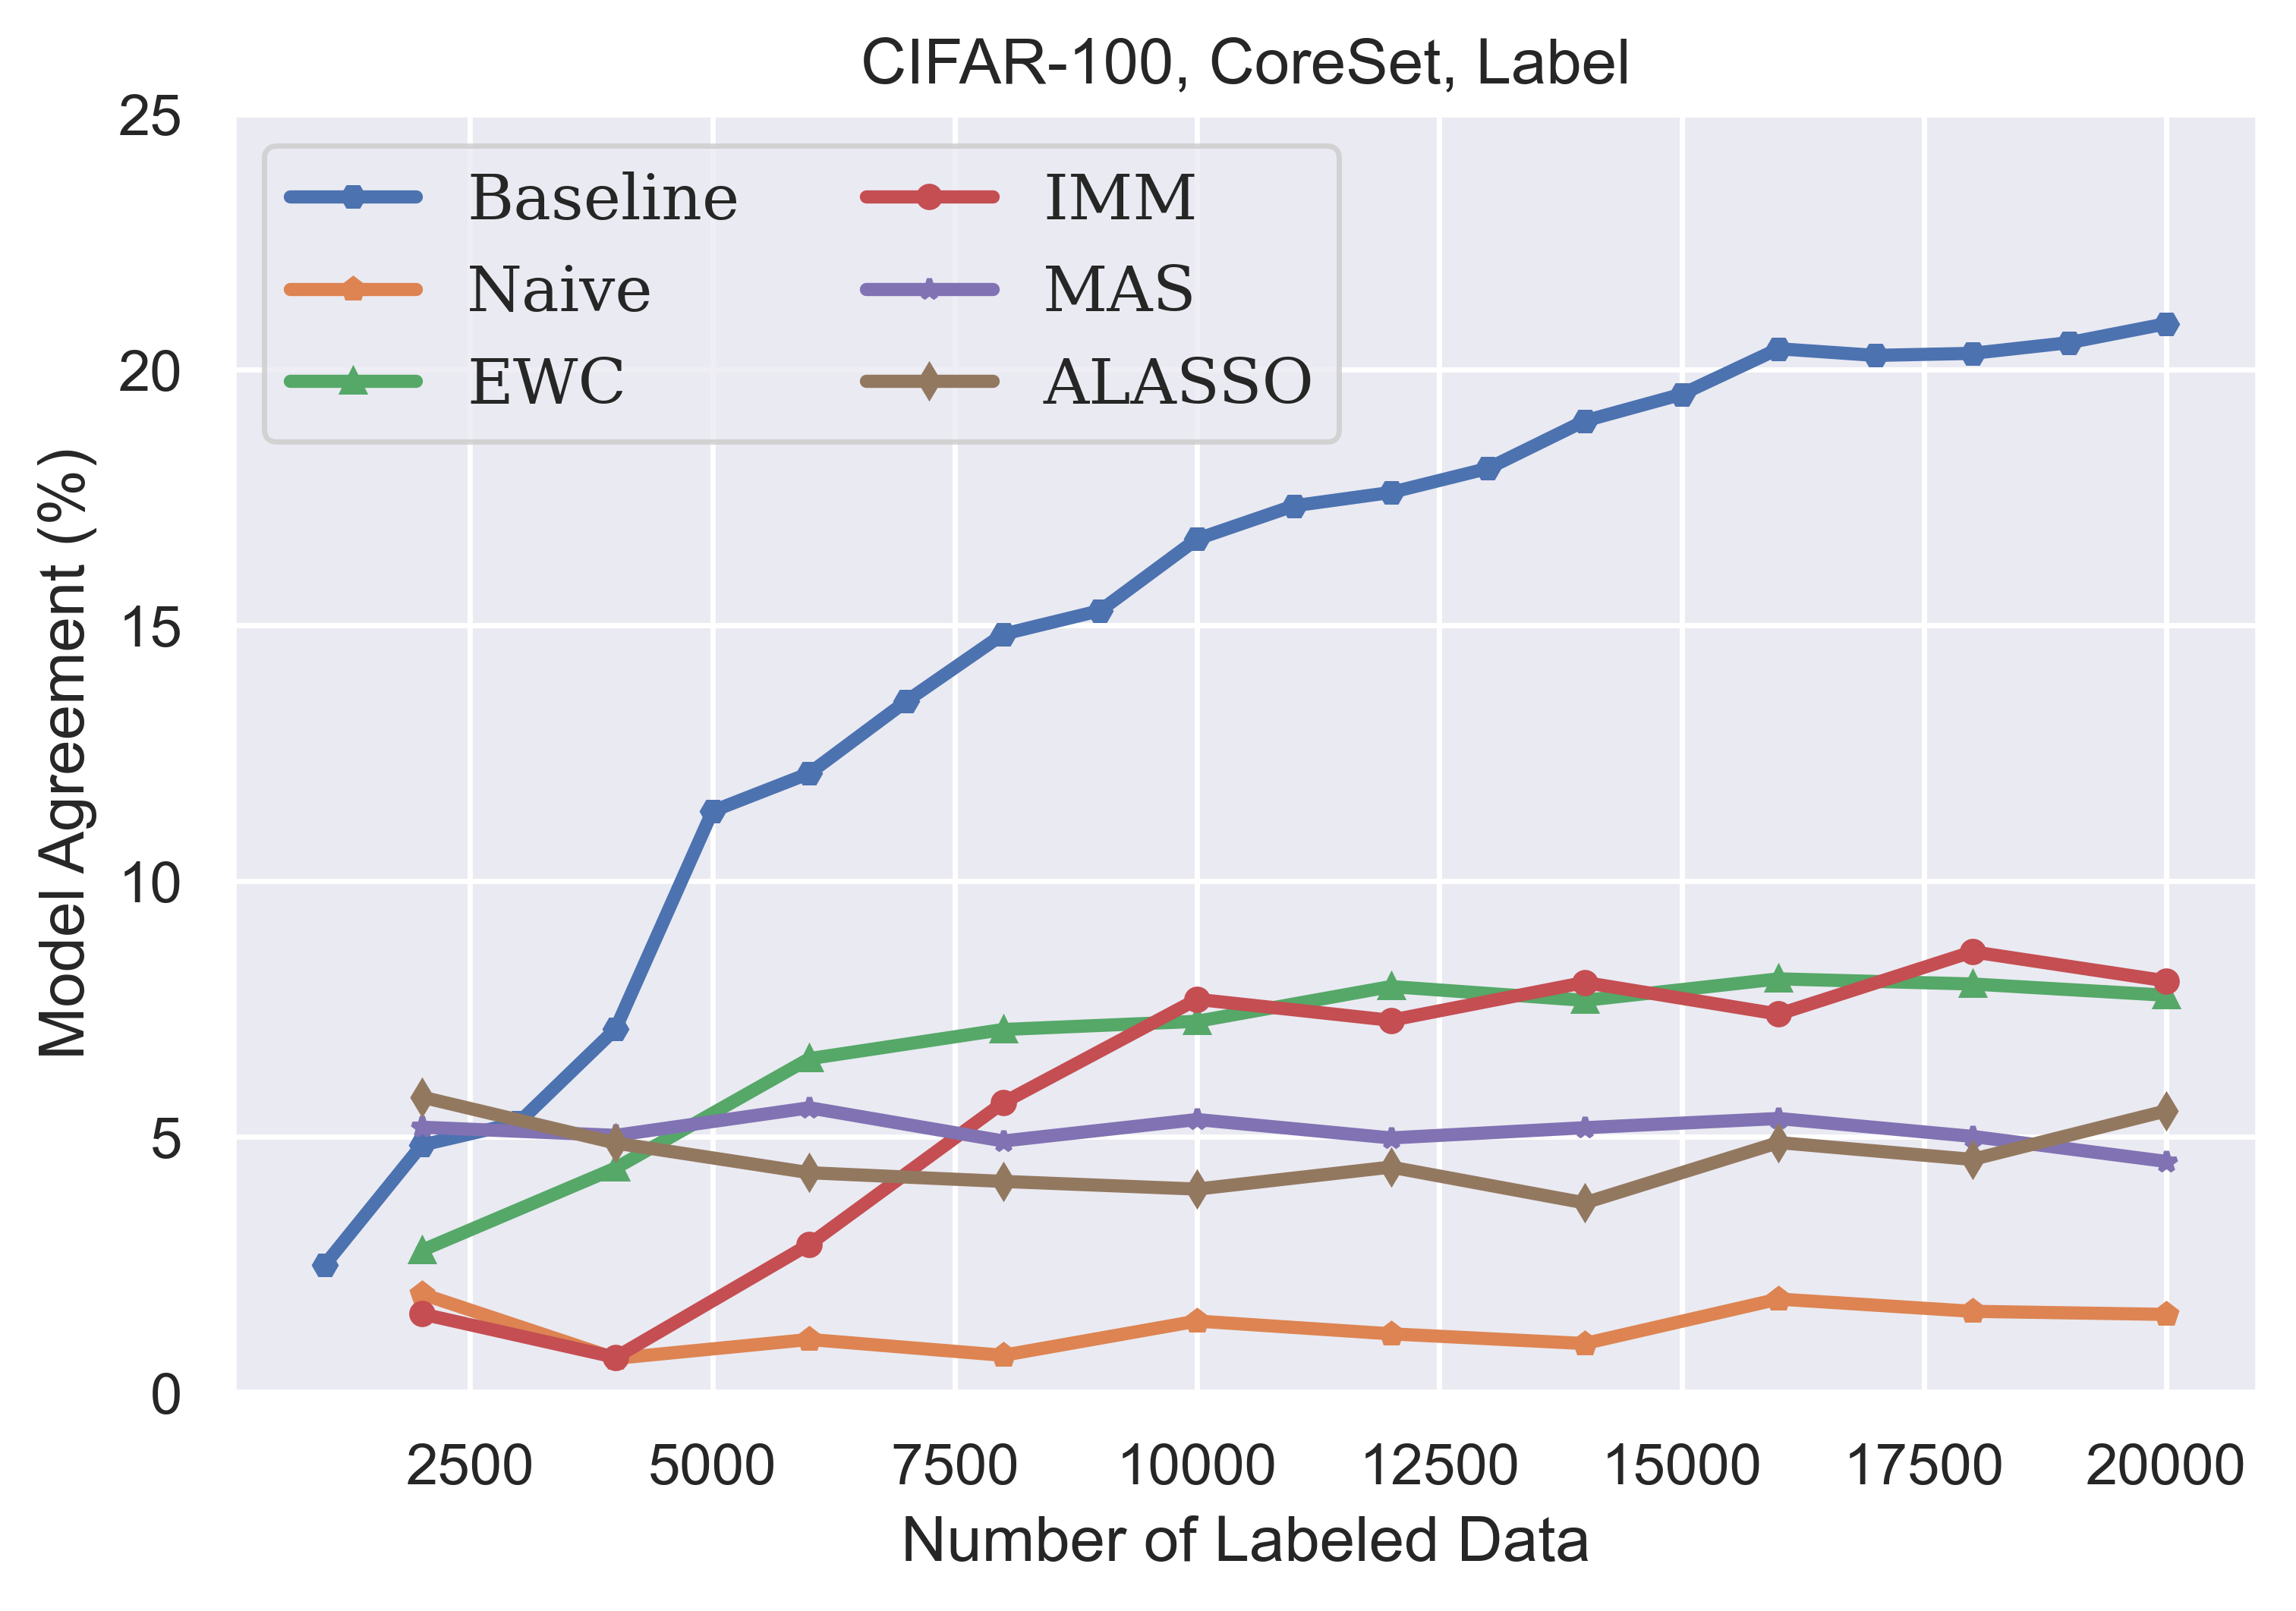
\includegraphics[width=0.8\linewidth]{images/results_CALMS/cifar100_label_coreset.png}
    \caption[Accuracy Comparison for Model Stealing on CIFAR10 using the top1-label and the Active Learning strategy CoreSet]{TODO: Nice text here}
    \label{fig:CALMSCIFAR10LabelCoreSet}
\end{figure}

\begin{figure}[h]
    \centering
    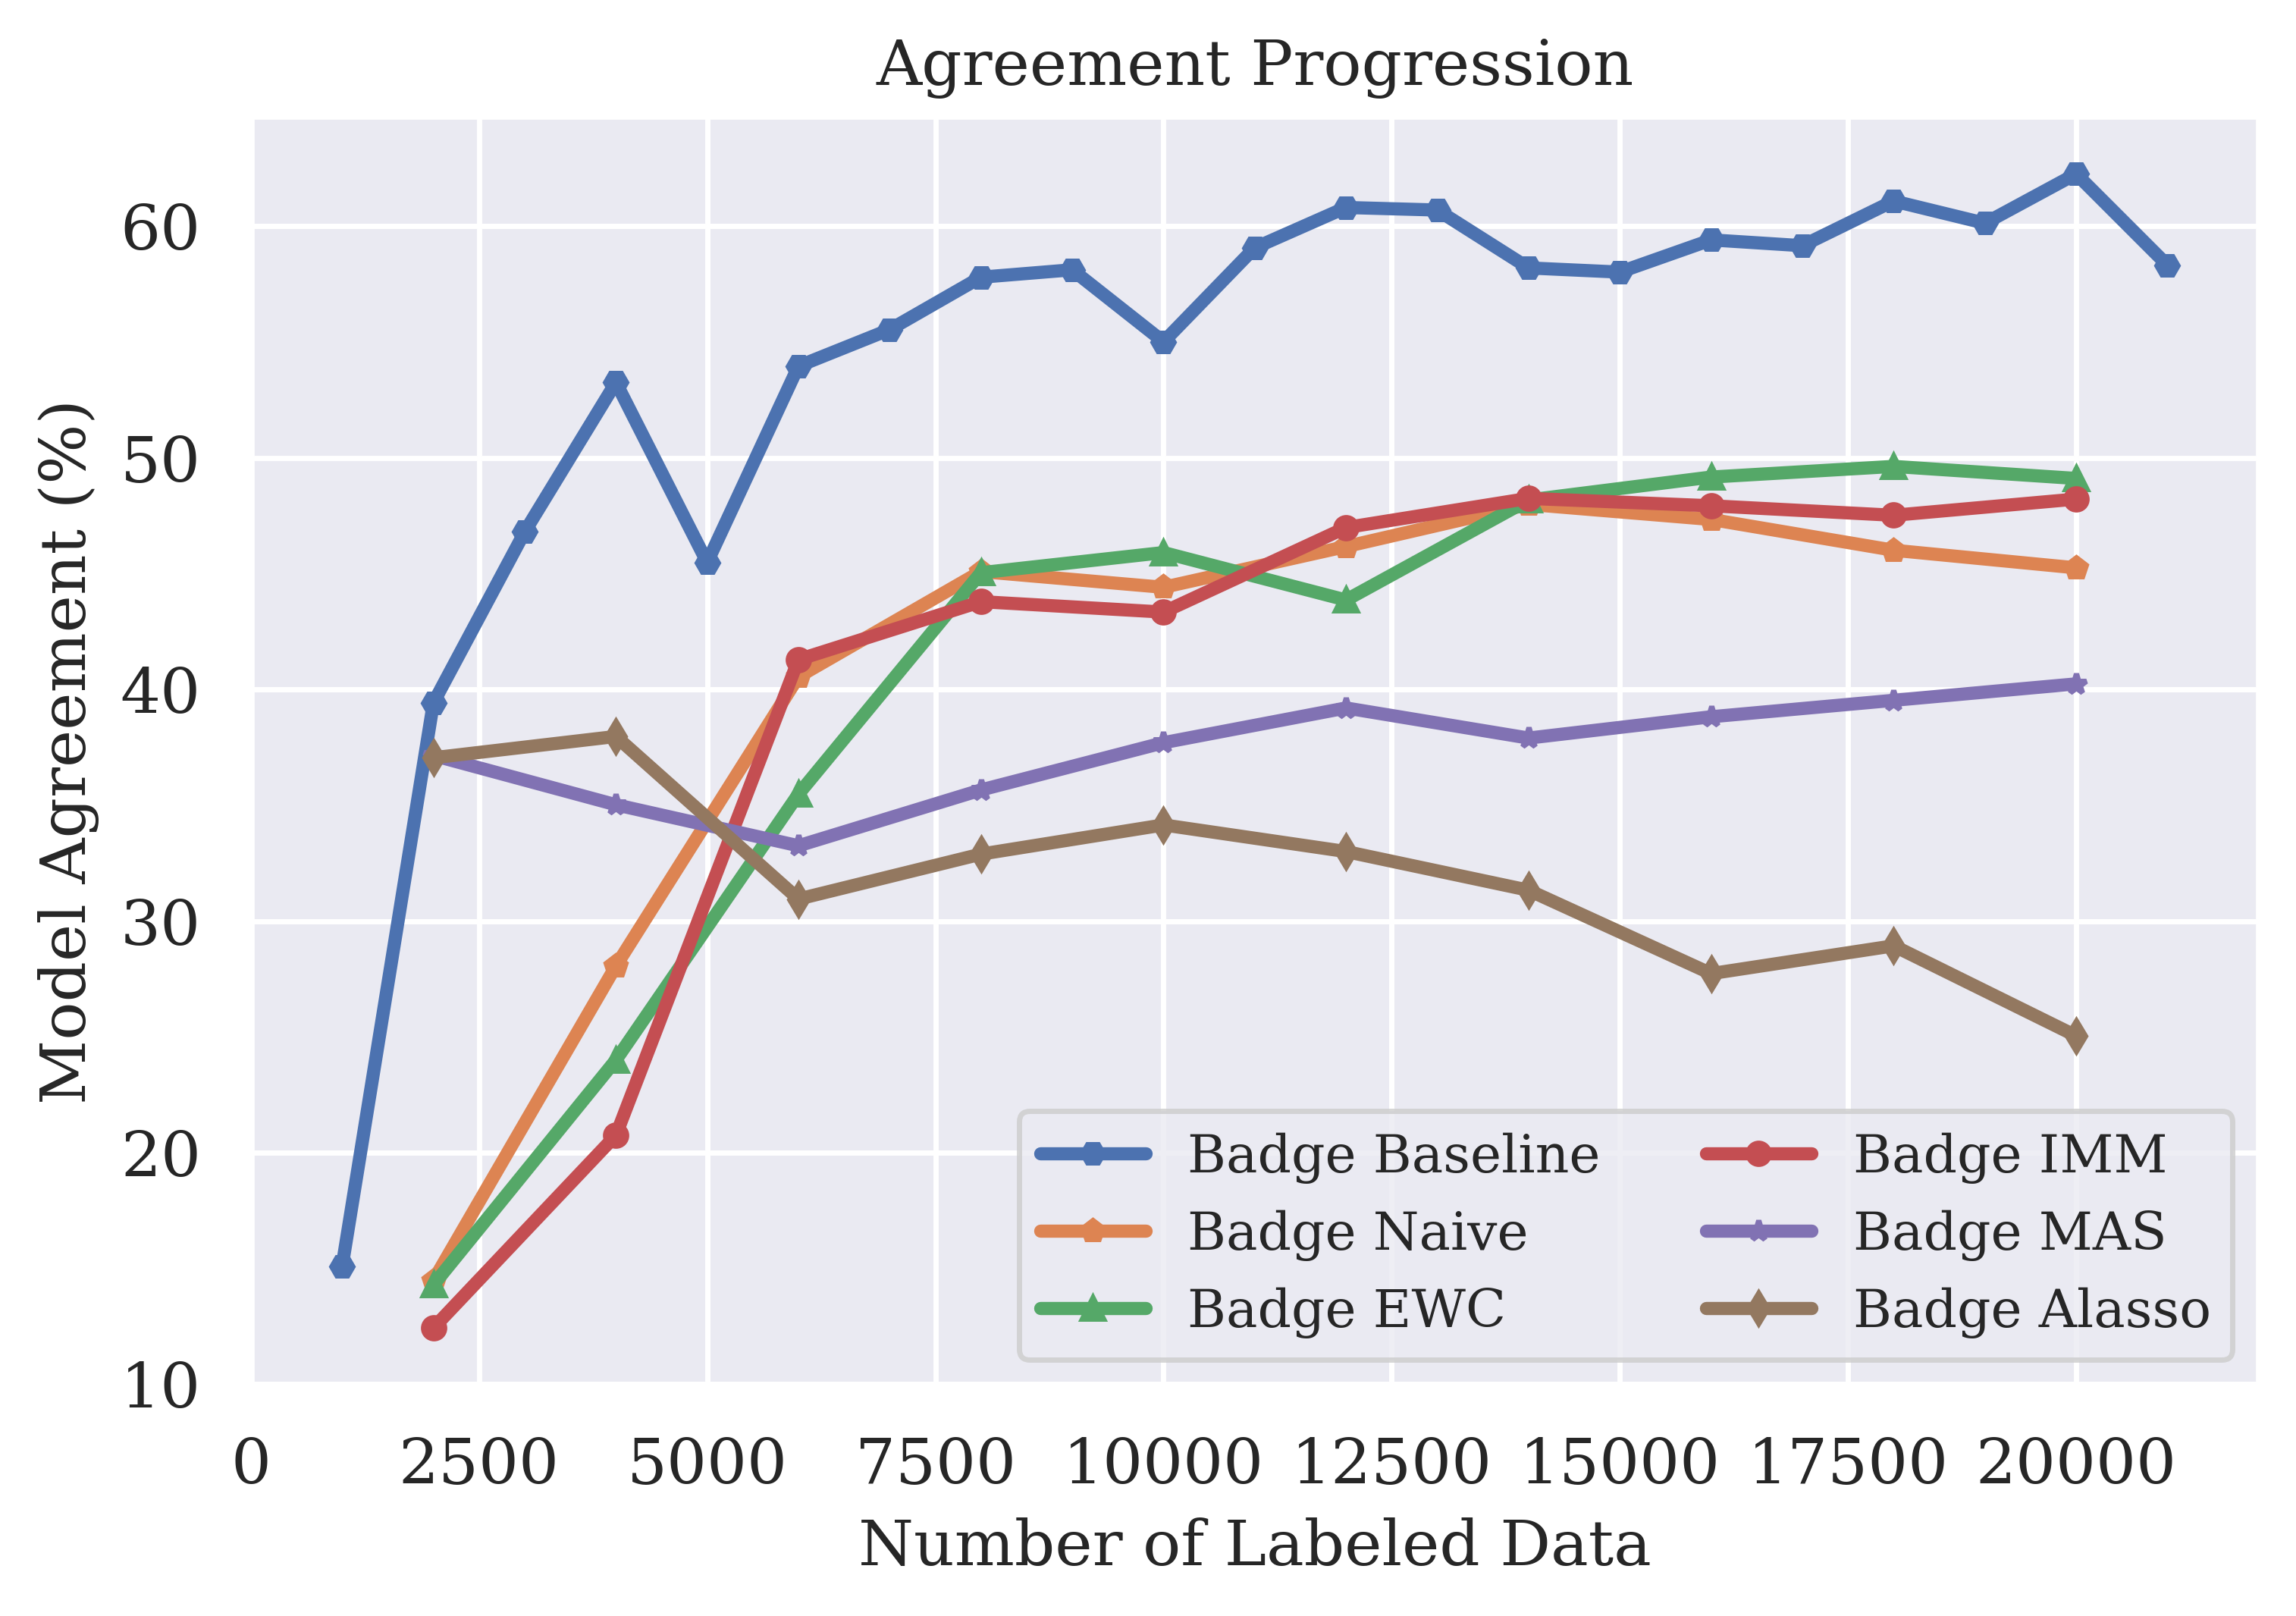
\includegraphics[width=0.8\linewidth]{images/results_CALMS/cifar_label_badge.png}
    \caption[Accuracy Comparison for Model Stealing on CIFAR10 using the top1-label and the Active Learning strategy Badge]{TODO: Nice text here}
    \label{fig:CALMSCIFAR10LabelBadge}
\end{figure}

%Softmax
\begin{figure}[h]
    \centering
    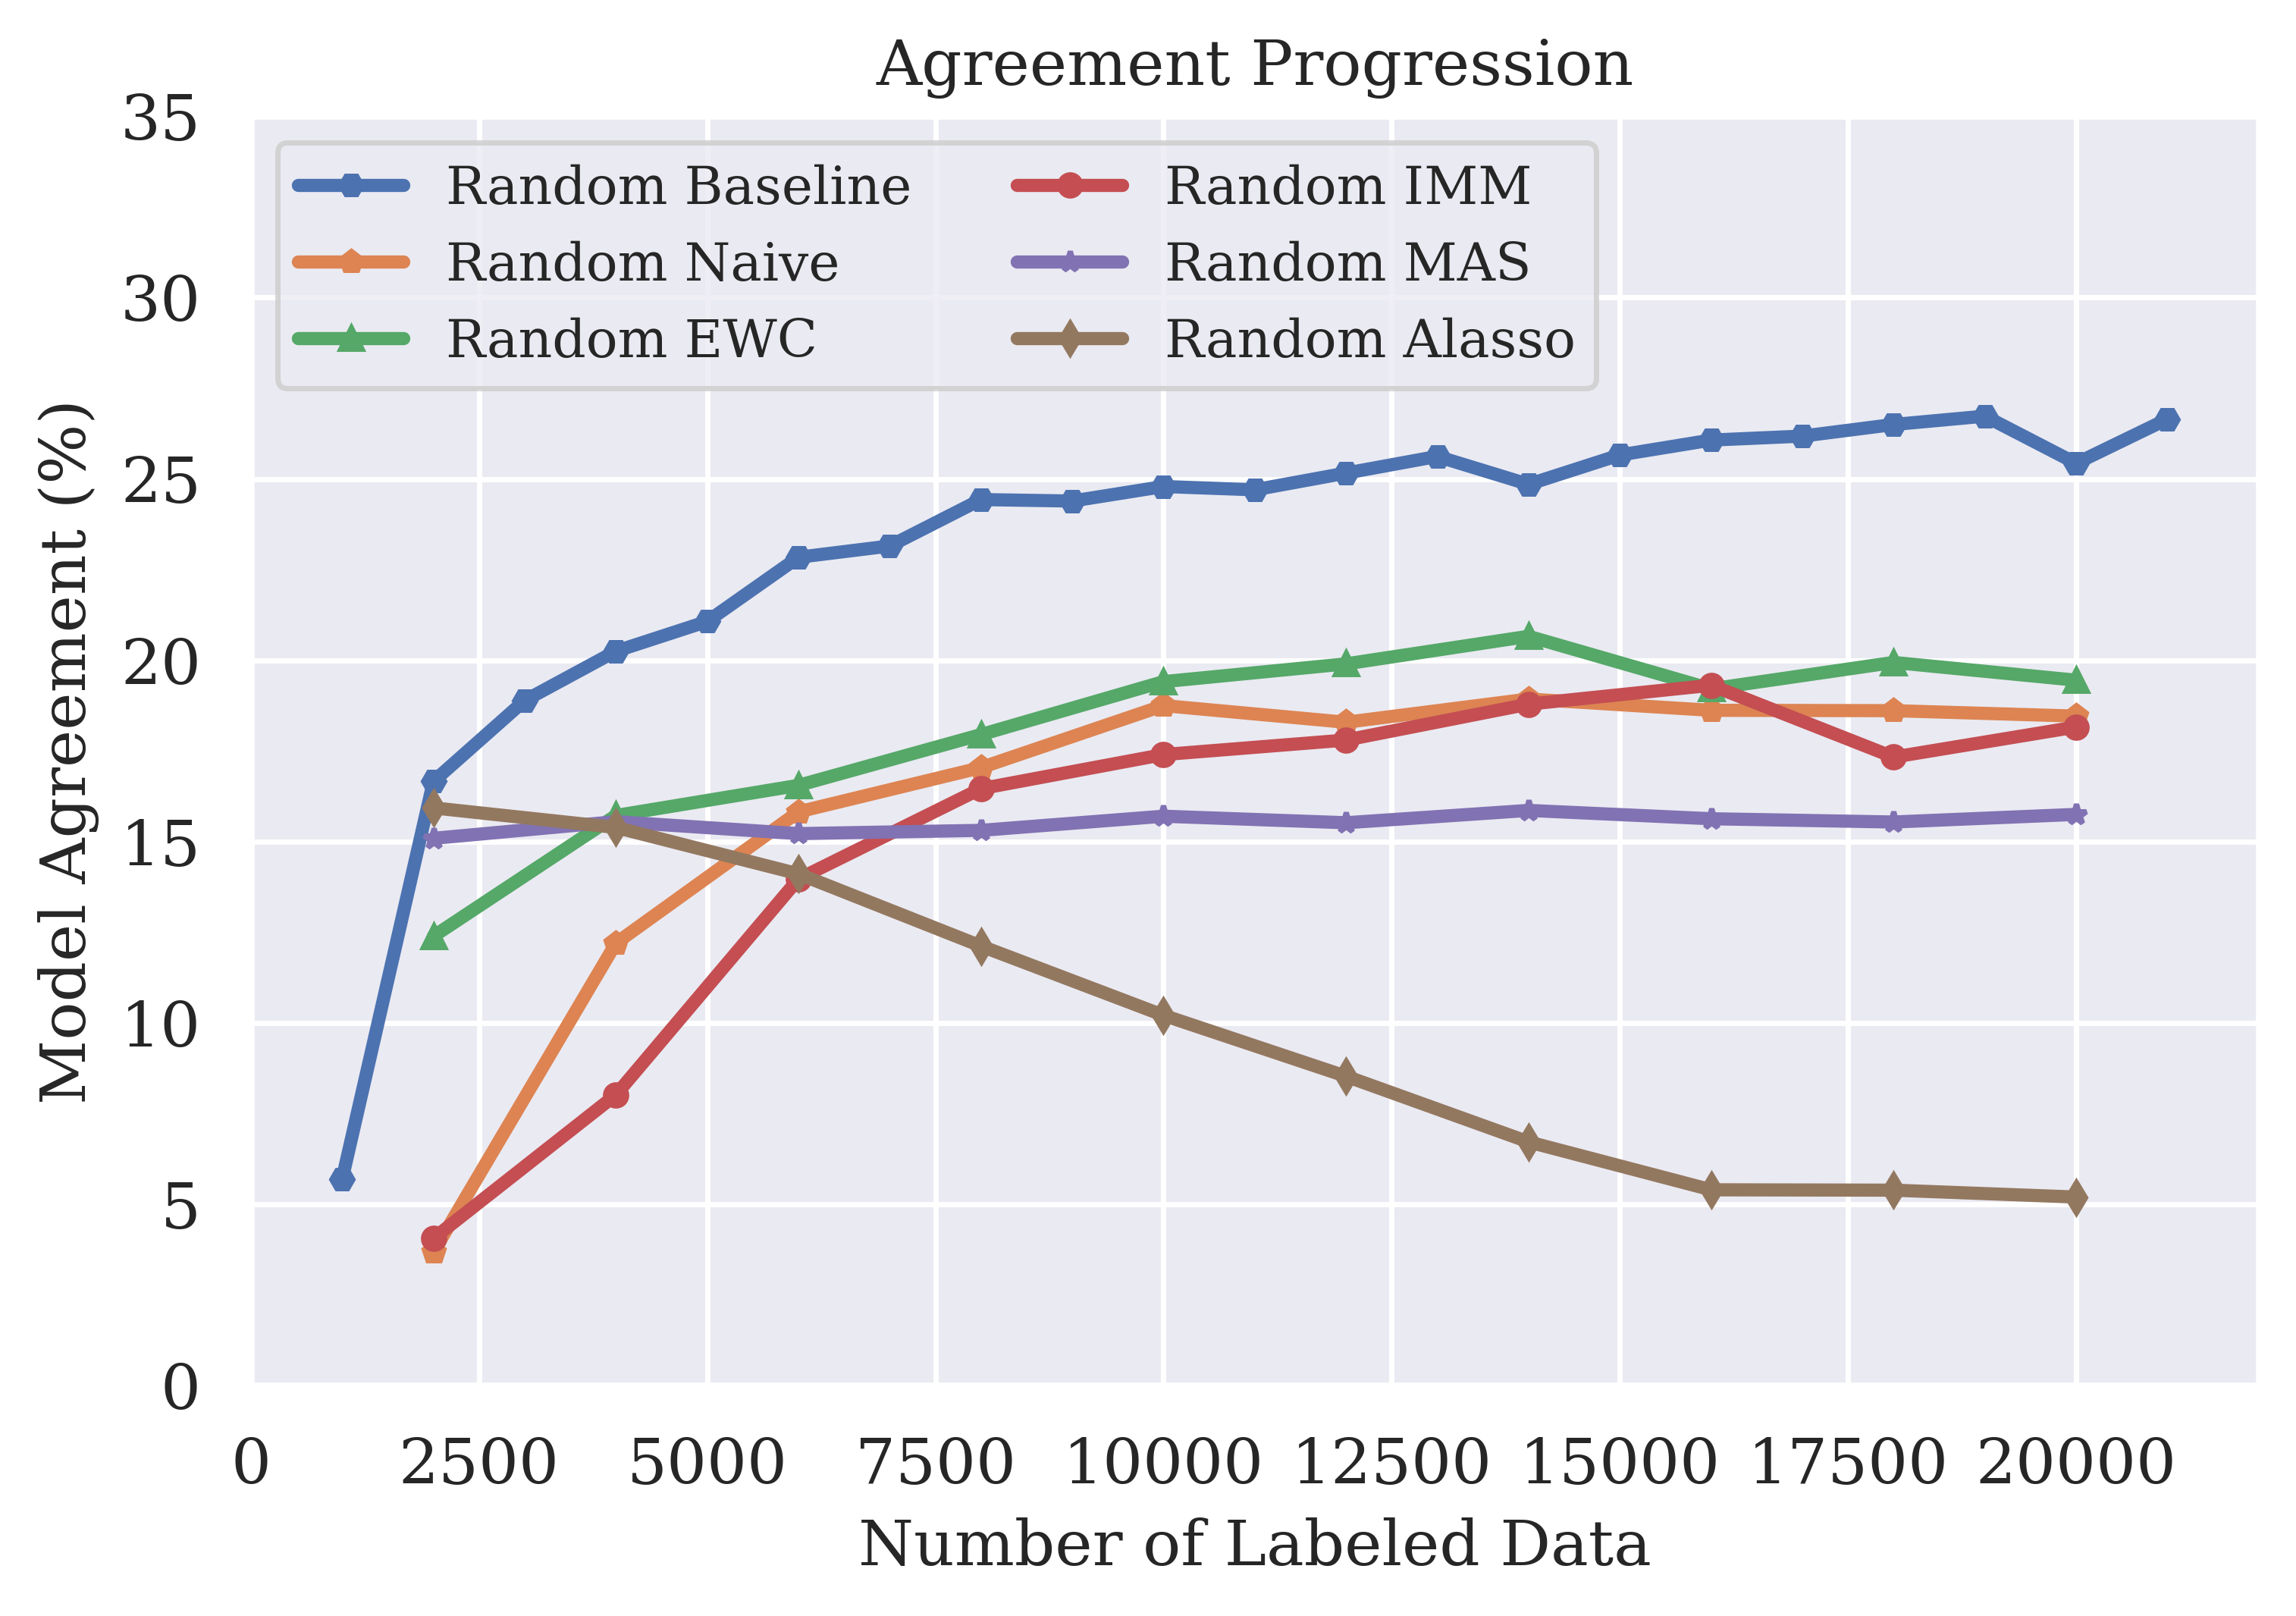
\includegraphics[width=0.8\linewidth]{images/results_CALMS/cifar100_softmax_random.png}
    \caption[Accuracy Comparison for Model Stealing on CIFAR10 using the softmax output and the Active Learning strategy Random]{TODO: Nice text here}
    \label{fig:CALMSCIFAR10SoftmaxRandom}
\end{figure}

\begin{figure}[h]
    \centering
    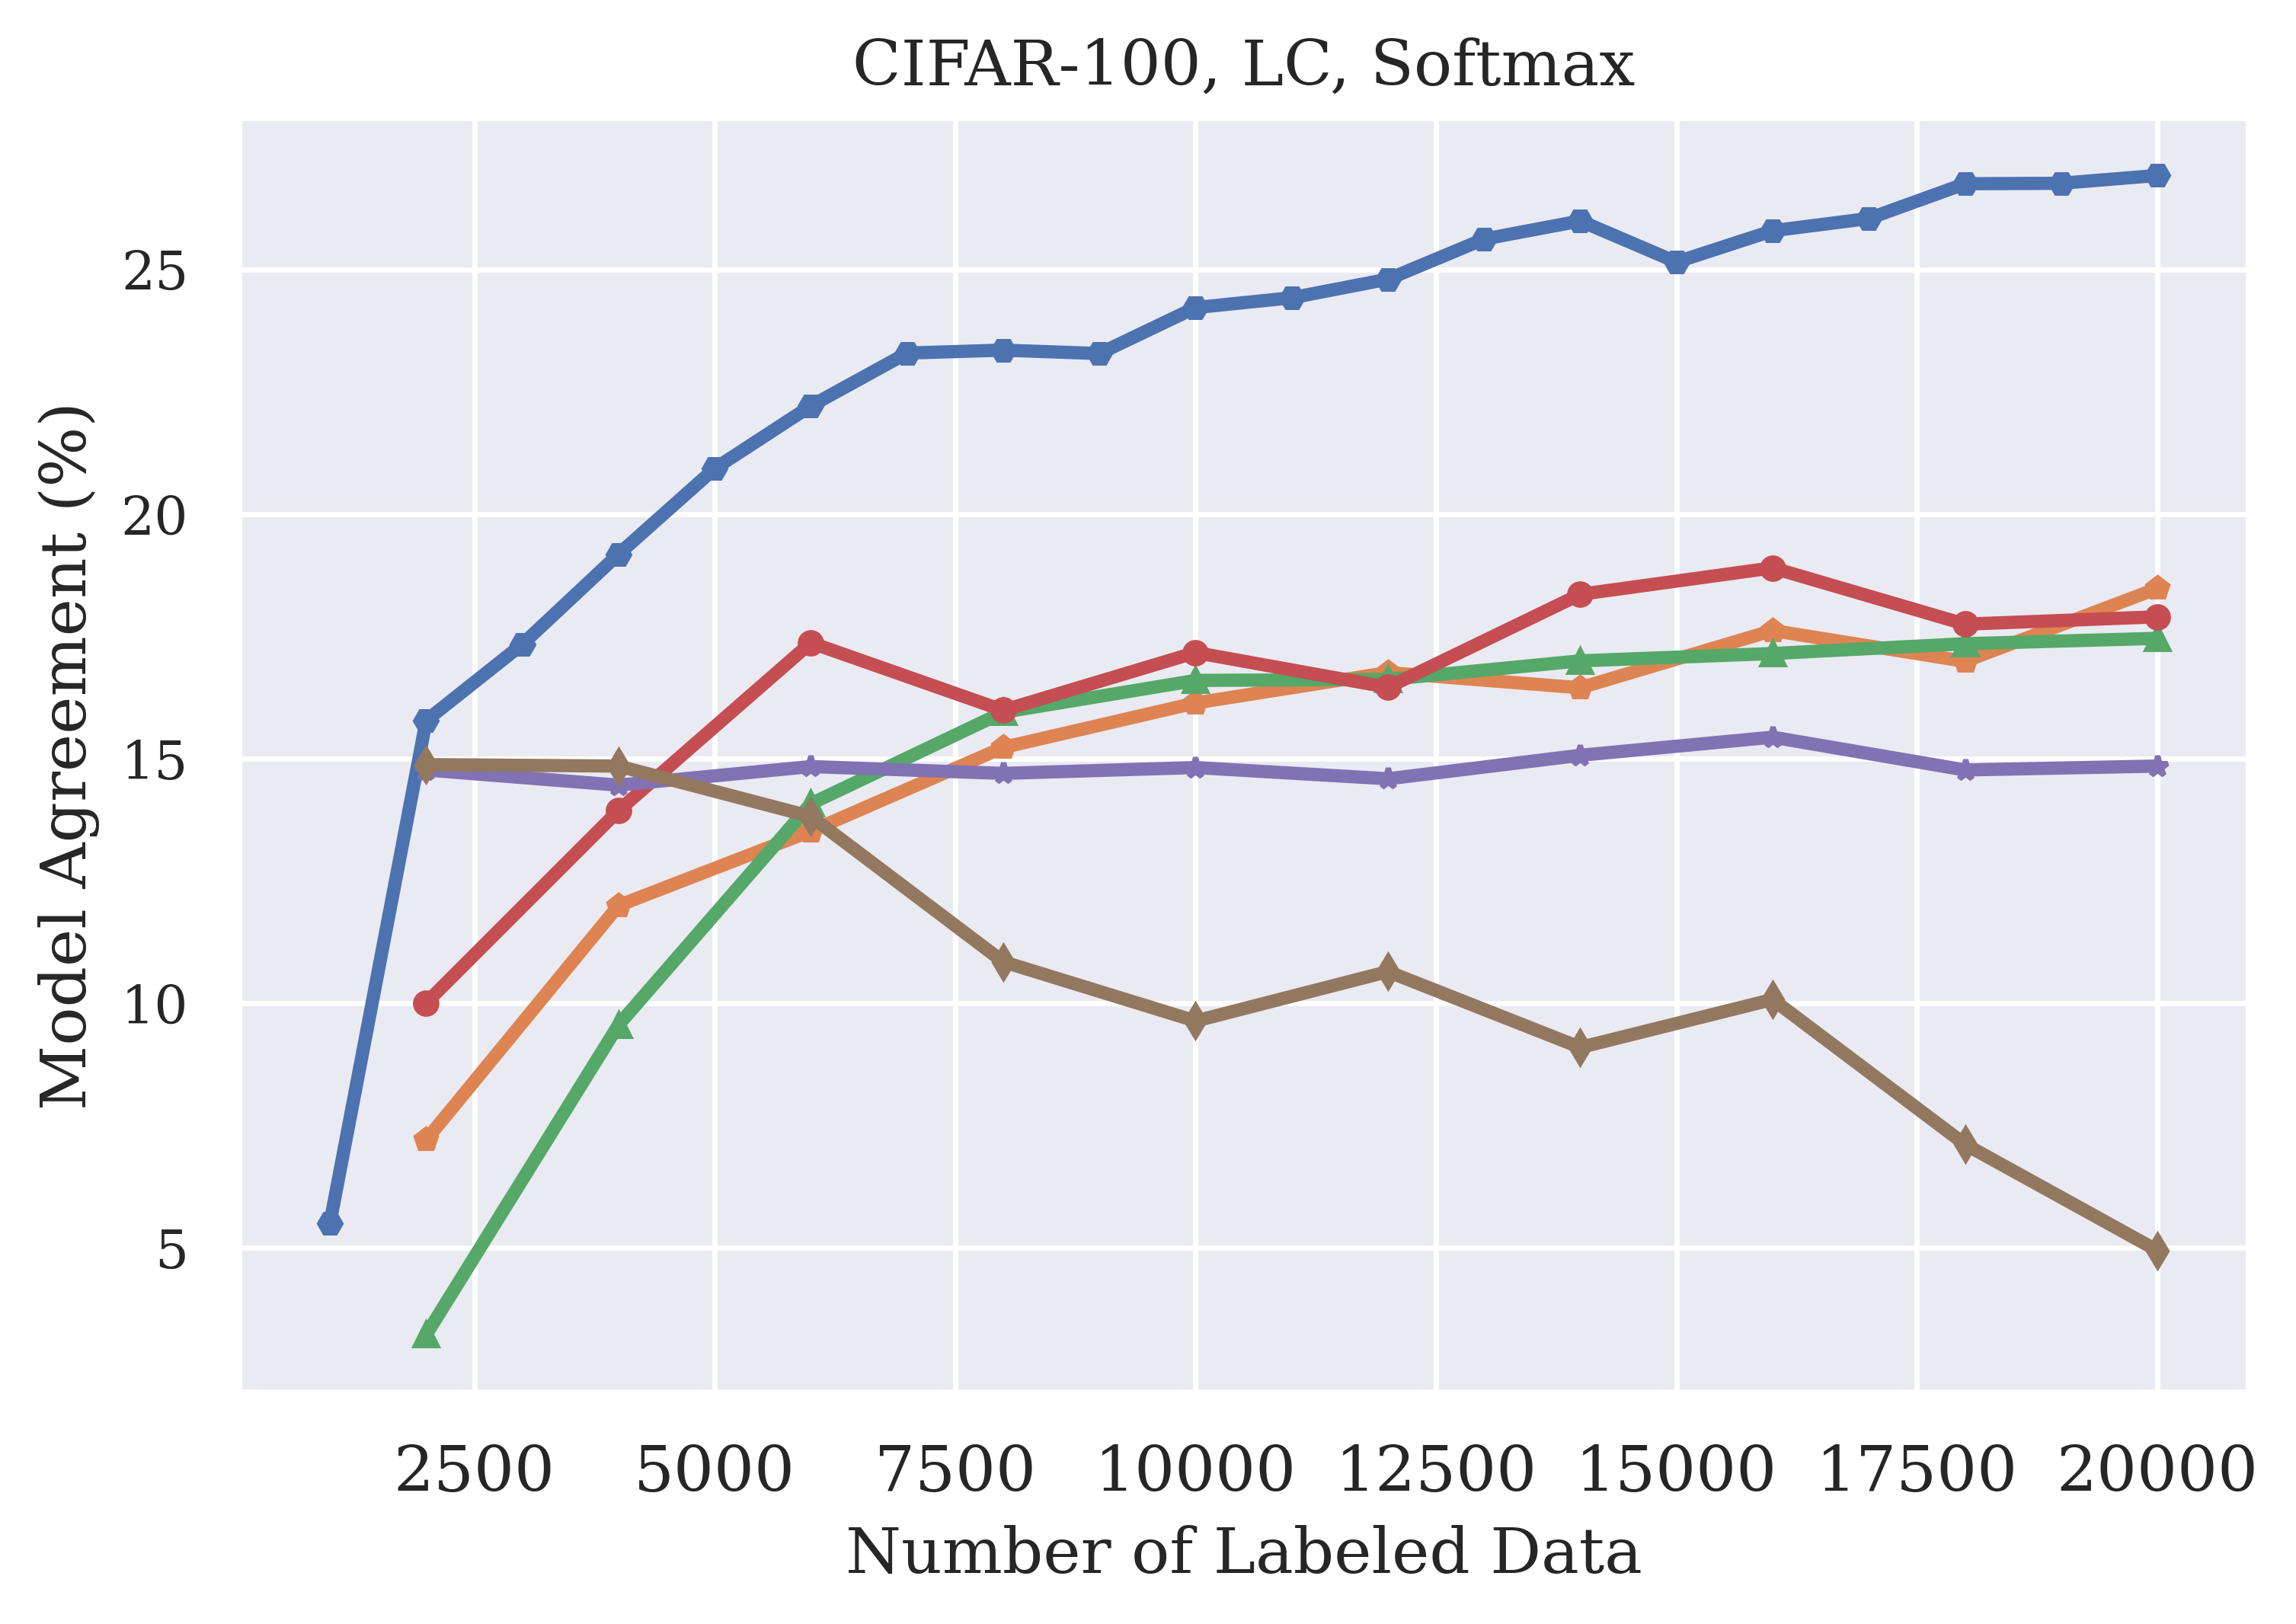
\includegraphics[width=0.8\linewidth]{images/results_CALMS/cifar100_softmax_lc.png}
    \caption[Accuracy Comparison for Model Stealing on CIFAR10 using the softmax output and the Active Learning strategy LC]{TODO: Nice text here}
    \label{fig:CALMSCIFAR10SoftmaxLC}
\end{figure}

\begin{figure}[h]
    \centering
    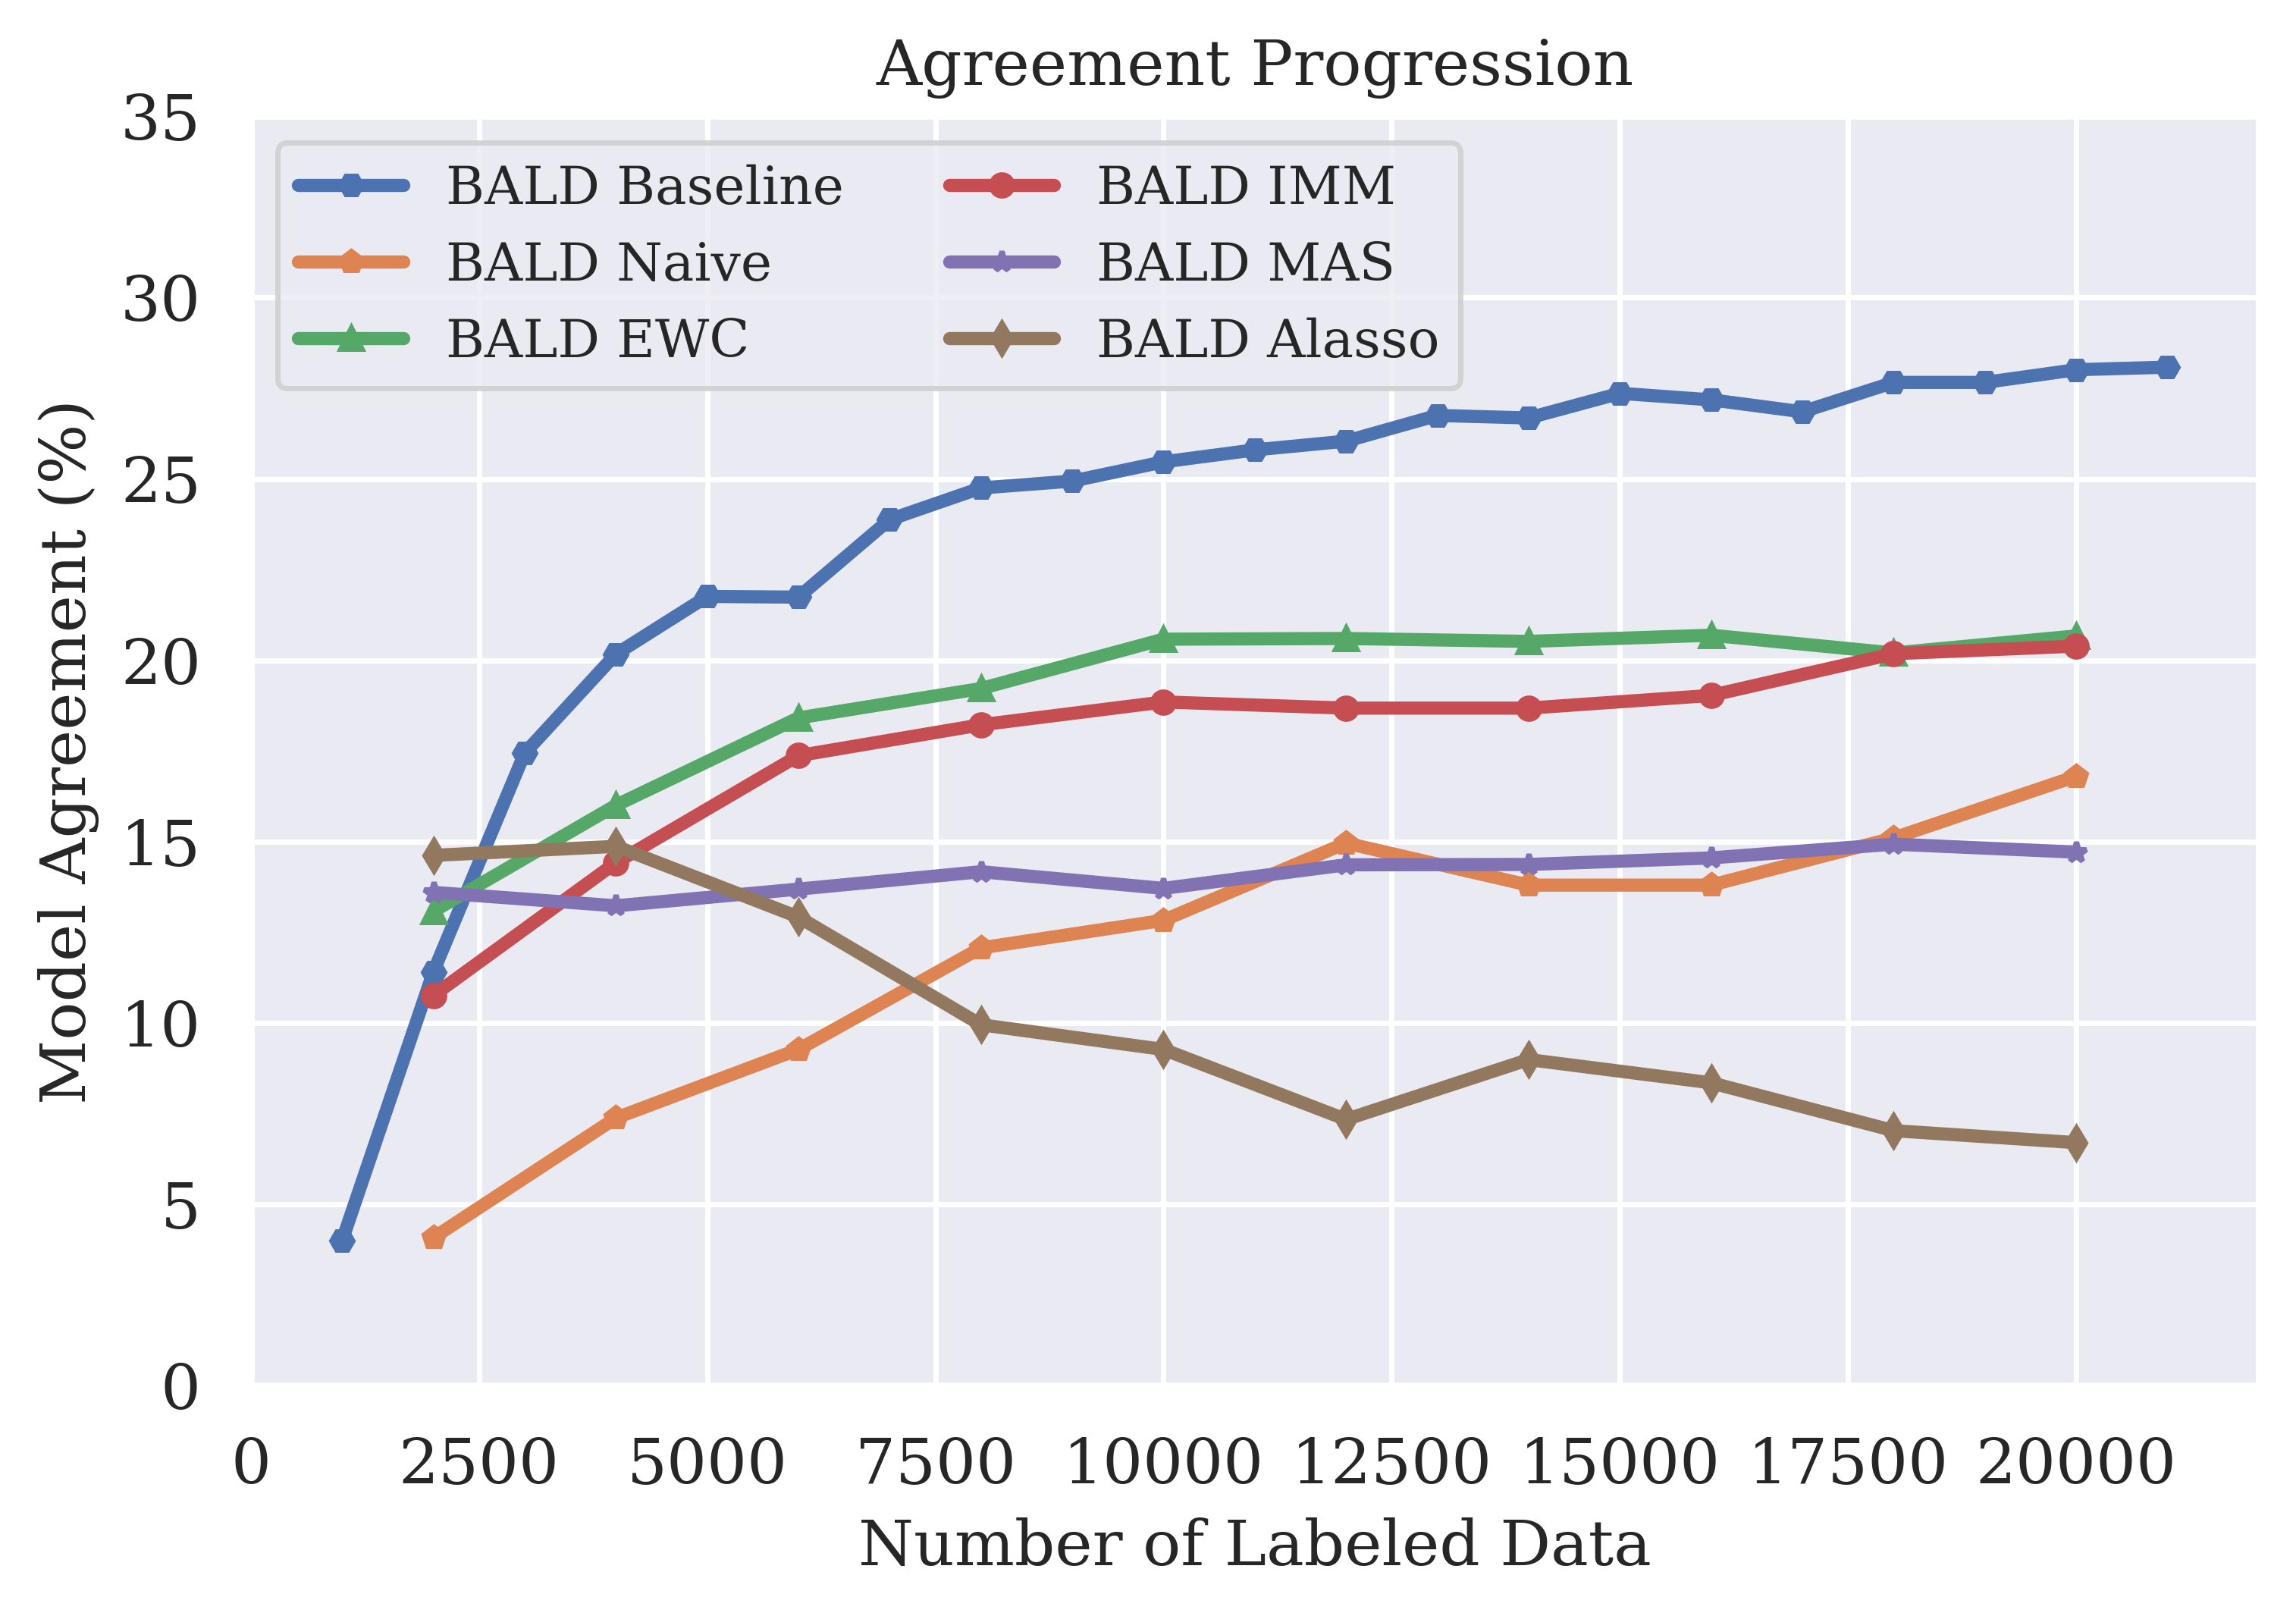
\includegraphics[width=0.8\linewidth]{images/results_CALMS/cifar100_softmax_bald.png}
    \caption[Accuracy Comparison for Model Stealing on CIFAR10 using the softmax output and the Active Learning strategy BALD]{TODO: Nice text here}
    \label{fig:CALMSCIFAR10SoftmaxBALD}
\end{figure}

\begin{figure}[h]
    \centering
    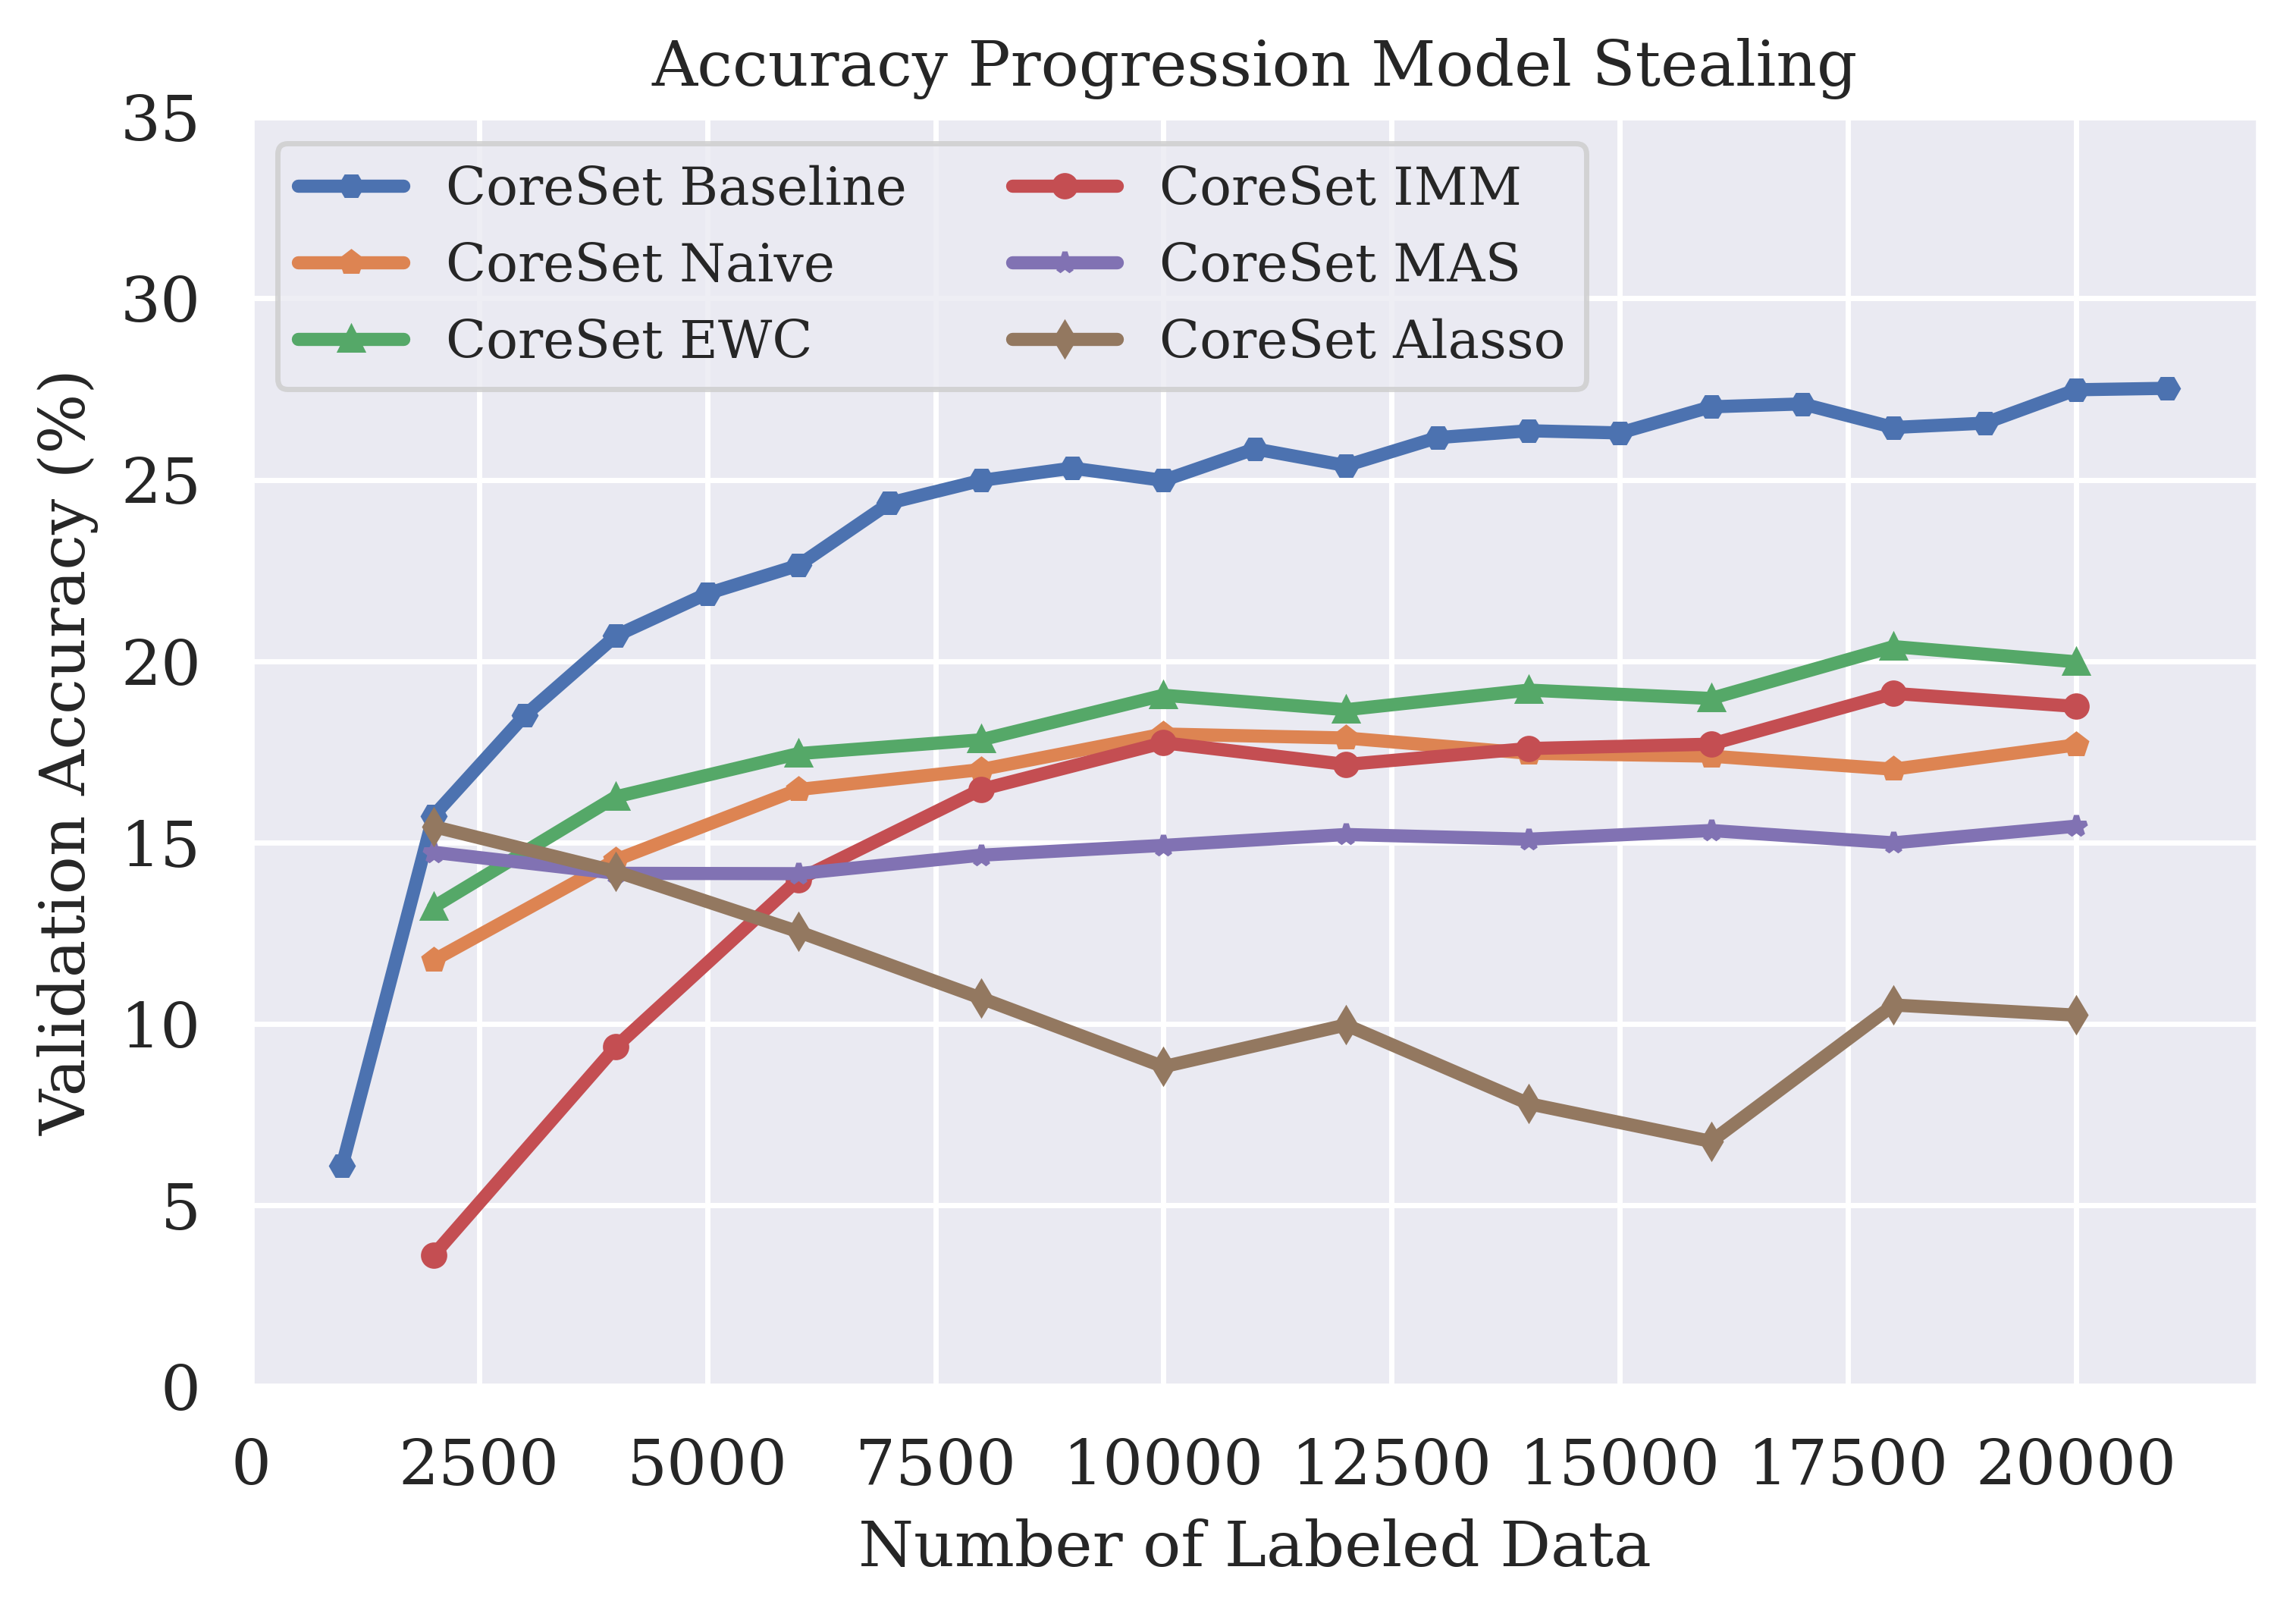
\includegraphics[width=0.8\linewidth]{images/results_CALMS/cifar100_softmax_coreset.png}
    \caption[Accuracy Comparison for Model Stealing on CIFAR10 using the softmax output and the Active Learning strategy CoreSet]{TODO: Nice text here}
    \label{fig:CALMSCIFAR10SoftmaxCoreSet}
\end{figure}

\begin{figure}[h]
    \centering
    \includegraphics[width=0.8\linewidth]{images/results_CALMS/cifar_softmax_badge.png}
    \caption[Accuracy Comparison for Model Stealing on CIFAR10 using the softmax output and the Active Learning strategy Badge]{TODO: Nice text here}
    \label{fig:CALMSCIFAR10SoftmaxBadge}
\end{figure}


%Tables for MNIST
%Label
\begin{figure}[h]
    \centering
    \includegraphics[width=0.8\linewidth]{images/results_CALMS/mnist_label_random.png}
    \caption[Accuracy Comparison for Model Stealing on MNIST using the top1-label and the Active Learning strategy Random]{TODO: Nice text here}
    \label{fig:CALMSMNISTLabelRandom}
\end{figure}

\begin{figure}[h]
    \centering
    \includegraphics[width=0.8\linewidth]{images/results_CALMS/mnist_label_lc.png}
    \caption[Accuracy Comparison for Model Stealing on MNIST using the top1-label and the Active Learning strategy LC]{TODO: Nice text here}
    \label{fig:CALMSMNISTLabelLC}
\end{figure}

% \begin{figure}[h]
%     \centering
%     \includegraphics[width=\linewidth]{images/results_CALMS/mnist_label_bald.png}
%     \caption[Accuracy Comparison for Model Stealing on MNIST using the top1-label and the Active Learning strategy BALD]{TODO: Nice text here}
%     \label{fig:CALMSMNISTLabelBALD}
% \end{figure}

\begin{figure}[h]
    \centering
    \includegraphics[width=0.8\linewidth]{images/results_CALMS/mnist_label_coreset.png}
    \caption[Accuracy Comparison for Model Stealing on MNIST using the top1-label and the Active Learning strategy CoreSet]{TODO: Nice text here}
    \label{fig:CALMSMNISTLabelCoreSet}
\end{figure}

\begin{figure}[h]
    \centering
    \includegraphics[width=0.8\linewidth]{images/results_CALMS/mnist_label_badge.png}
    \caption[Accuracy Comparison for Model Stealing on MNIST using the top1-label and the Active Learning strategy Badge]{TODO: Nice text here}
    \label{fig:CALMSMNISTLabelBadge}
\end{figure}

%Softmax
\begin{figure}[h]
    \centering
    \includegraphics[width=0.8\linewidth]{images/results_CALMS/mnist_softmax_random.png}
    \caption[Accuracy Comparison for Model Stealing on MNIST using the softmax output and the Active Learning strategy Random]{TODO: Nice text here}
    \label{fig:CALMSMNISTSoftmaxRandom}
\end{figure}

\begin{figure}[h]
    \centering
    \includegraphics[width=0.8\linewidth]{images/results_CALMS/mnist_softmax_lc.png}
    \caption[Accuracy Comparison for Model Stealing on MNIST using the softmax output and the Active Learning strategy LC]{TODO: Nice text here}
    \label{fig:CALMSMNISTSoftmaxLC}
\end{figure}

\begin{figure}[h]
    \centering
    \includegraphics[width=0.8\linewidth]{images/results_CALMS/mnist_softmax_bald.png}
    \caption[Accuracy Comparison for Model Stealing on MNIST using the softmax output and the Active Learning strategy BALD]{TODO: Nice text here}
    \label{fig:CALMSMNISTSoftmaxBALD}
\end{figure}

\begin{figure}[h]
    \centering
    \includegraphics[width=0.8\linewidth]{images/results_CALMS/mnist_softmax_coreset.png}
    \caption[Accuracy Comparison for Model Stealing on MNIST using the softmax output and the Active Learning strategy CoreSet]{TODO: Nice text here}
    \label{fig:CALMSMNISTSoftmaxCoreSet}
\end{figure}

\begin{figure}[h]
    \centering
    \includegraphics[width=0.8\linewidth]{images/results_CALMS/cifar_softmax_badge.png}
    \caption[Accuracy Comparison for Model Stealing on MNIST using the softmax output and the Active Learning strategy Badge]{TODO: Nice text here}
    \label{fig:CALMSMNISTSoftmaxBadge}
\end{figure}

%TODO: Hier VAAL AGEM einfügen

\end{document}
